\documentclass[twoside]{book}

% Packages required by doxygen
\usepackage{fixltx2e}
\usepackage{calc}
\usepackage{doxygen}
\usepackage[export]{adjustbox} % also loads graphicx
\usepackage{graphicx}
\usepackage[utf8]{inputenc}
\usepackage{makeidx}
\usepackage{multicol}
\usepackage{multirow}
\PassOptionsToPackage{warn}{textcomp}
\usepackage{textcomp}
\usepackage[nointegrals]{wasysym}
\usepackage[table]{xcolor}

% Font selection
\usepackage[T1]{fontenc}
\usepackage[scaled=.90]{helvet}
\usepackage{courier}
\usepackage{amssymb}
\usepackage{sectsty}
\renewcommand{\familydefault}{\sfdefault}
\allsectionsfont{%
  \fontseries{bc}\selectfont%
  \color{darkgray}%
}
\renewcommand{\DoxyLabelFont}{%
  \fontseries{bc}\selectfont%
  \color{darkgray}%
}
\newcommand{\+}{\discretionary{\mbox{\scriptsize$\hookleftarrow$}}{}{}}

% Page & text layout
\usepackage{geometry}
\geometry{%
  a4paper,%
  top=2.5cm,%
  bottom=2.5cm,%
  left=2.5cm,%
  right=2.5cm%
}
\tolerance=750
\hfuzz=15pt
\hbadness=750
\setlength{\emergencystretch}{15pt}
\setlength{\parindent}{0cm}
\setlength{\parskip}{0.2cm}
\makeatletter
\renewcommand{\paragraph}{%
  \@startsection{paragraph}{4}{0ex}{-1.0ex}{1.0ex}{%
    \normalfont\normalsize\bfseries\SS@parafont%
  }%
}
\renewcommand{\subparagraph}{%
  \@startsection{subparagraph}{5}{0ex}{-1.0ex}{1.0ex}{%
    \normalfont\normalsize\bfseries\SS@subparafont%
  }%
}
\makeatother

% Headers & footers
\usepackage{fancyhdr}
\pagestyle{fancyplain}
\fancyhead[LE]{\fancyplain{}{\bfseries\thepage}}
\fancyhead[CE]{\fancyplain{}{}}
\fancyhead[RE]{\fancyplain{}{\bfseries\leftmark}}
\fancyhead[LO]{\fancyplain{}{\bfseries\rightmark}}
\fancyhead[CO]{\fancyplain{}{}}
\fancyhead[RO]{\fancyplain{}{\bfseries\thepage}}
\fancyfoot[LE]{\fancyplain{}{}}
\fancyfoot[CE]{\fancyplain{}{}}
\fancyfoot[RE]{\fancyplain{}{\bfseries\scriptsize Generated on Fri Sep 18 2015 11\+:10\+:47 for Social\+Proximity\+Library by Doxygen }}
\fancyfoot[LO]{\fancyplain{}{\bfseries\scriptsize Generated on Fri Sep 18 2015 11\+:10\+:47 for Social\+Proximity\+Library by Doxygen }}
\fancyfoot[CO]{\fancyplain{}{}}
\fancyfoot[RO]{\fancyplain{}{}}
\renewcommand{\footrulewidth}{0.4pt}
\renewcommand{\chaptermark}[1]{%
  \markboth{#1}{}%
}
\renewcommand{\sectionmark}[1]{%
  \markright{\thesection\ #1}%
}

% Indices & bibliography
\usepackage{natbib}
\usepackage[titles]{tocloft}
\setcounter{tocdepth}{3}
\setcounter{secnumdepth}{5}
\makeindex

% Hyperlinks (required, but should be loaded last)
\usepackage{ifpdf}
\ifpdf
  \usepackage[pdftex,pagebackref=true]{hyperref}
\else
  \usepackage[ps2pdf,pagebackref=true]{hyperref}
\fi
\hypersetup{%
  colorlinks=true,%
  linkcolor=blue,%
  citecolor=blue,%
  unicode%
}

% Custom commands
\newcommand{\clearemptydoublepage}{%
  \newpage{\pagestyle{empty}\cleardoublepage}%
}


%===== C O N T E N T S =====

\begin{document}

% Titlepage & ToC
\hypersetup{pageanchor=false,
             bookmarks=true,
             bookmarksnumbered=true,
             pdfencoding=unicode
            }
\pagenumbering{roman}
\begin{titlepage}
\vspace*{7cm}
\begin{center}%
{\Large Social\+Proximity\+Library }\\
\vspace*{1cm}
{\large Generated by Doxygen 1.8.10}\\
\vspace*{0.5cm}
{\small Fri Sep 18 2015 11:10:47}\\
\end{center}
\end{titlepage}
\clearemptydoublepage
\tableofcontents
\clearemptydoublepage
\pagenumbering{arabic}
\hypersetup{pageanchor=true}

%--- Begin generated contents ---
\chapter{Namespace Index}
\section{Packages}
Here are the packages with brief descriptions (if available)\+:\begin{DoxyCompactList}
\item\contentsline{section}{\hyperlink{namespacecom}{com} }{\pageref{namespacecom}}{}
\item\contentsline{section}{\hyperlink{namespacecom_1_1copelabs}{com.\+copelabs} }{\pageref{namespacecom_1_1copelabs}}{}
\item\contentsline{section}{\hyperlink{namespacecom_1_1copelabs_1_1oiframework}{com.\+copelabs.\+oiframework} }{\pageref{namespacecom_1_1copelabs_1_1oiframework}}{}
\item\contentsline{section}{\hyperlink{namespacecom_1_1copelabs_1_1oiframework_1_1bt}{com.\+copelabs.\+oiframework.\+bt} }{\pageref{namespacecom_1_1copelabs_1_1oiframework_1_1bt}}{}
\item\contentsline{section}{\hyperlink{namespacecom_1_1copelabs_1_1oiframework_1_1contentmanager}{com.\+copelabs.\+oiframework.\+contentmanager} }{\pageref{namespacecom_1_1copelabs_1_1oiframework_1_1contentmanager}}{}
\item\contentsline{section}{\hyperlink{namespacecom_1_1copelabs_1_1oiframework_1_1router}{com.\+copelabs.\+oiframework.\+router} }{\pageref{namespacecom_1_1copelabs_1_1oiframework_1_1router}}{}
\item\contentsline{section}{\hyperlink{namespacecom_1_1copelabs_1_1oiframework_1_1socialproximity}{com.\+copelabs.\+oiframework.\+socialproximity} }{\pageref{namespacecom_1_1copelabs_1_1oiframework_1_1socialproximity}}{}
\item\contentsline{section}{\hyperlink{namespacecom_1_1copelabs_1_1oiframework_1_1wifi}{com.\+copelabs.\+oiframework.\+wifi} }{\pageref{namespacecom_1_1copelabs_1_1oiframework_1_1wifi}}{}
\end{DoxyCompactList}

\chapter{Hierarchical Index}
\section{Class Hierarchy}
This inheritance list is sorted roughly, but not completely, alphabetically\+:\begin{DoxyCompactList}
\item \contentsline{section}{com.\+copelabs.\+oiframework.\+bt.\+Bluetooth\+Manager}{\pageref{classcom_1_1copelabs_1_1oiframework_1_1bt_1_1_bluetooth_manager}}{}
\item \contentsline{section}{com.\+copelabs.\+oiframework.\+bt.\+B\+T\+Device\+Finder}{\pageref{interfacecom_1_1copelabs_1_1oiframework_1_1bt_1_1_b_t_device_finder}}{}
\item \contentsline{section}{com.\+copelabs.\+oiframework.\+socialproximity.\+Data\+Base}{\pageref{classcom_1_1copelabs_1_1oiframework_1_1socialproximity_1_1_data_base}}{}
\item \contentsline{section}{com.\+copelabs.\+oiframework.\+socialproximity.\+Data\+Base\+Change\+Listener}{\pageref{interfacecom_1_1copelabs_1_1oiframework_1_1socialproximity_1_1_data_base_change_listener}}{}
\item \contentsline{section}{com.\+copelabs.\+oiframework.\+wifi.\+Wifi\+Direct\+Auto\+Accept.\+Dialog\+Listener\+Proxy}{\pageref{classcom_1_1copelabs_1_1oiframework_1_1wifi_1_1_wifi_direct_auto_accept_1_1_dialog_listener_proxy}}{}
\item \contentsline{section}{com.\+copelabs.\+oiframework.\+contentmanager.\+File\+I\+O}{\pageref{classcom_1_1copelabs_1_1oiframework_1_1contentmanager_1_1_file_i_o}}{}
\item \contentsline{section}{com.\+copelabs.\+oiframework.\+router.\+Routing}{\pageref{classcom_1_1copelabs_1_1oiframework_1_1router_1_1_routing}}{}
\item \contentsline{section}{com.\+copelabs.\+oiframework.\+router.\+Routing\+Listener}{\pageref{interfacecom_1_1copelabs_1_1oiframework_1_1router_1_1_routing_listener}}{}
\item Runnable\begin{DoxyCompactList}
\item \contentsline{section}{com.\+copelabs.\+oiframework.\+wifi.\+Send\+Data}{\pageref{classcom_1_1copelabs_1_1oiframework_1_1wifi_1_1_send_data}}{}
\end{DoxyCompactList}
\item \contentsline{section}{com.\+copelabs.\+oiframework.\+socialproximity.\+Social\+Proximity}{\pageref{classcom_1_1copelabs_1_1oiframework_1_1socialproximity_1_1_social_proximity}}{}
\item \contentsline{section}{com.\+copelabs.\+oiframework.\+socialproximity.\+Social\+Proximity\+Listener}{\pageref{interfacecom_1_1copelabs_1_1oiframework_1_1socialproximity_1_1_social_proximity_listener}}{}
\item Thread\begin{DoxyCompactList}
\item \contentsline{section}{com.\+copelabs.\+oiframework.\+wifi.\+Client\+Socket\+Handler}{\pageref{classcom_1_1copelabs_1_1oiframework_1_1wifi_1_1_client_socket_handler}}{}
\item \contentsline{section}{com.\+copelabs.\+oiframework.\+wifi.\+Server\+Thread}{\pageref{classcom_1_1copelabs_1_1oiframework_1_1wifi_1_1_server_thread}}{}
\end{DoxyCompactList}
\item \contentsline{section}{com.\+copelabs.\+oiframework.\+socialproximity.\+User\+Dev\+Average\+Encounter\+Duration}{\pageref{classcom_1_1copelabs_1_1oiframework_1_1socialproximity_1_1_user_dev_average_encounter_duration}}{}
\item \contentsline{section}{com.\+copelabs.\+oiframework.\+socialproximity.\+User\+Dev\+Encounter\+Duration}{\pageref{classcom_1_1copelabs_1_1oiframework_1_1socialproximity_1_1_user_dev_encounter_duration}}{}
\item \contentsline{section}{com.\+copelabs.\+oiframework.\+socialproximity.\+User\+Device\+Info}{\pageref{classcom_1_1copelabs_1_1oiframework_1_1socialproximity_1_1_user_device_info}}{}
\item \contentsline{section}{com.\+copelabs.\+oiframework.\+socialproximity.\+User\+Dev\+Social\+Weight}{\pageref{classcom_1_1copelabs_1_1oiframework_1_1socialproximity_1_1_user_dev_social_weight}}{}
\item \contentsline{section}{com.\+copelabs.\+oiframework.\+wifi.\+Wi\+Fi\+Direct}{\pageref{classcom_1_1copelabs_1_1oiframework_1_1wifi_1_1_wi_fi_direct}}{}
\item \contentsline{section}{com.\+copelabs.\+oiframework.\+wifi.\+Wifi\+Direct\+Auto\+Accept}{\pageref{classcom_1_1copelabs_1_1oiframework_1_1wifi_1_1_wifi_direct_auto_accept}}{}
\item \contentsline{section}{com.\+copelabs.\+oiframework.\+wifi.\+Wi\+Fi\+Direct\+Device}{\pageref{classcom_1_1copelabs_1_1oiframework_1_1wifi_1_1_wi_fi_direct_device}}{}
\item \contentsline{section}{com.\+copelabs.\+oiframework.\+wifi.\+Wi\+Fi\+Direct\+Listener}{\pageref{interfacecom_1_1copelabs_1_1oiframework_1_1wifi_1_1_wi_fi_direct_listener}}{}
\item \contentsline{section}{com.\+copelabs.\+oiframework.\+contentmanager.\+Xml\+Pull\+Parser\+Handler}{\pageref{classcom_1_1copelabs_1_1oiframework_1_1contentmanager_1_1_xml_pull_parser_handler}}{}
\item Broadcast\+Receiver\begin{DoxyCompactList}
\item \contentsline{section}{com.\+copelabs.\+oiframework.\+socialproximity.\+On\+Social\+Weight\+Update}{\pageref{classcom_1_1copelabs_1_1oiframework_1_1socialproximity_1_1_on_social_weight_update}}{}
\item \contentsline{section}{com.\+copelabs.\+oiframework.\+wifi.\+Wi\+Fi\+Direct\+Broadcast\+Receiver}{\pageref{classcom_1_1copelabs_1_1oiframework_1_1wifi_1_1_wi_fi_direct_broadcast_receiver}}{}
\end{DoxyCompactList}
\item Callback\begin{DoxyCompactList}
\item \contentsline{section}{com.\+copelabs.\+oiframework.\+wifi.\+Wi\+Fi\+Direct\+Utils}{\pageref{classcom_1_1copelabs_1_1oiframework_1_1wifi_1_1_wi_fi_direct_utils}}{}
\end{DoxyCompactList}
\item Comparator\begin{DoxyCompactList}
\item \contentsline{section}{com.\+copelabs.\+oiframework.\+socialproximity.\+Social\+Proximity.\+Custom\+Comparator}{\pageref{classcom_1_1copelabs_1_1oiframework_1_1socialproximity_1_1_social_proximity_1_1_custom_comparator}}{}
\end{DoxyCompactList}
\item Connection\+Info\+Listener\begin{DoxyCompactList}
\item \contentsline{section}{com.\+copelabs.\+oiframework.\+wifi.\+Wi\+Fi\+Direct\+Utils}{\pageref{classcom_1_1copelabs_1_1oiframework_1_1wifi_1_1_wi_fi_direct_utils}}{}
\end{DoxyCompactList}
\item Parcelable\begin{DoxyCompactList}
\item \contentsline{section}{com.\+copelabs.\+oiframework.\+socialproximity.\+Social\+Weight}{\pageref{classcom_1_1copelabs_1_1oiframework_1_1socialproximity_1_1_social_weight}}{}
\end{DoxyCompactList}
\item Peer\+List\+Listener\begin{DoxyCompactList}
\item \contentsline{section}{com.\+copelabs.\+oiframework.\+wifi.\+Wi\+Fi\+Direct\+Utils}{\pageref{classcom_1_1copelabs_1_1oiframework_1_1wifi_1_1_wi_fi_direct_utils}}{}
\end{DoxyCompactList}
\item Serializable\begin{DoxyCompactList}
\item \contentsline{section}{com.\+copelabs.\+oiframework.\+contentmanager.\+Packet}{\pageref{classcom_1_1copelabs_1_1oiframework_1_1contentmanager_1_1_packet}}{}
\end{DoxyCompactList}
\item Service\begin{DoxyCompactList}
\item \contentsline{section}{com.\+copelabs.\+oiframework.\+contentmanager.\+Content\+Manager}{\pageref{classcom_1_1copelabs_1_1oiframework_1_1contentmanager_1_1_content_manager}}{}
\end{DoxyCompactList}
\item S\+Q\+Lite\+Open\+Helper\begin{DoxyCompactList}
\item \contentsline{section}{com.\+copelabs.\+oiframework.\+socialproximity.\+S\+Q\+Lite\+Helper}{\pageref{classcom_1_1copelabs_1_1oiframework_1_1socialproximity_1_1_s_q_lite_helper}}{}
\end{DoxyCompactList}
\item Timer\+Task\begin{DoxyCompactList}
\item \contentsline{section}{com.\+copelabs.\+oiframework.\+contentmanager.\+Clean\+Task}{\pageref{classcom_1_1copelabs_1_1oiframework_1_1contentmanager_1_1_clean_task}}{}
\end{DoxyCompactList}
\end{DoxyCompactList}

\chapter{Class Index}
\section{Class List}
Here are the classes, structs, unions and interfaces with brief descriptions\+:\begin{DoxyCompactList}
\item\contentsline{section}{\hyperlink{classcom_1_1copelabs_1_1oiframework_1_1bt_1_1_bluetooth_manager}{com.\+copelabs.\+oiframework.\+bt.\+Bluetooth\+Manager} }{\pageref{classcom_1_1copelabs_1_1oiframework_1_1bt_1_1_bluetooth_manager}}{}
\item\contentsline{section}{\hyperlink{interfacecom_1_1copelabs_1_1oiframework_1_1bt_1_1_b_t_device_finder}{com.\+copelabs.\+oiframework.\+bt.\+B\+T\+Device\+Finder} }{\pageref{interfacecom_1_1copelabs_1_1oiframework_1_1bt_1_1_b_t_device_finder}}{}
\item\contentsline{section}{\hyperlink{classcom_1_1copelabs_1_1oiframework_1_1contentmanager_1_1_clean_task}{com.\+copelabs.\+oiframework.\+contentmanager.\+Clean\+Task} }{\pageref{classcom_1_1copelabs_1_1oiframework_1_1contentmanager_1_1_clean_task}}{}
\item\contentsline{section}{\hyperlink{classcom_1_1copelabs_1_1oiframework_1_1wifi_1_1_client_socket_handler}{com.\+copelabs.\+oiframework.\+wifi.\+Client\+Socket\+Handler} }{\pageref{classcom_1_1copelabs_1_1oiframework_1_1wifi_1_1_client_socket_handler}}{}
\item\contentsline{section}{\hyperlink{classcom_1_1copelabs_1_1oiframework_1_1contentmanager_1_1_content_manager}{com.\+copelabs.\+oiframework.\+contentmanager.\+Content\+Manager} }{\pageref{classcom_1_1copelabs_1_1oiframework_1_1contentmanager_1_1_content_manager}}{}
\item\contentsline{section}{\hyperlink{classcom_1_1copelabs_1_1oiframework_1_1socialproximity_1_1_social_proximity_1_1_custom_comparator}{com.\+copelabs.\+oiframework.\+socialproximity.\+Social\+Proximity.\+Custom\+Comparator} }{\pageref{classcom_1_1copelabs_1_1oiframework_1_1socialproximity_1_1_social_proximity_1_1_custom_comparator}}{}
\item\contentsline{section}{\hyperlink{classcom_1_1copelabs_1_1oiframework_1_1socialproximity_1_1_data_base}{com.\+copelabs.\+oiframework.\+socialproximity.\+Data\+Base} }{\pageref{classcom_1_1copelabs_1_1oiframework_1_1socialproximity_1_1_data_base}}{}
\item\contentsline{section}{\hyperlink{interfacecom_1_1copelabs_1_1oiframework_1_1socialproximity_1_1_data_base_change_listener}{com.\+copelabs.\+oiframework.\+socialproximity.\+Data\+Base\+Change\+Listener} }{\pageref{interfacecom_1_1copelabs_1_1oiframework_1_1socialproximity_1_1_data_base_change_listener}}{}
\item\contentsline{section}{\hyperlink{classcom_1_1copelabs_1_1oiframework_1_1wifi_1_1_wifi_direct_auto_accept_1_1_dialog_listener_proxy}{com.\+copelabs.\+oiframework.\+wifi.\+Wifi\+Direct\+Auto\+Accept.\+Dialog\+Listener\+Proxy} }{\pageref{classcom_1_1copelabs_1_1oiframework_1_1wifi_1_1_wifi_direct_auto_accept_1_1_dialog_listener_proxy}}{}
\item\contentsline{section}{\hyperlink{classcom_1_1copelabs_1_1oiframework_1_1contentmanager_1_1_file_i_o}{com.\+copelabs.\+oiframework.\+contentmanager.\+File\+I\+O} }{\pageref{classcom_1_1copelabs_1_1oiframework_1_1contentmanager_1_1_file_i_o}}{}
\item\contentsline{section}{\hyperlink{classcom_1_1copelabs_1_1oiframework_1_1socialproximity_1_1_on_social_weight_update}{com.\+copelabs.\+oiframework.\+socialproximity.\+On\+Social\+Weight\+Update} }{\pageref{classcom_1_1copelabs_1_1oiframework_1_1socialproximity_1_1_on_social_weight_update}}{}
\item\contentsline{section}{\hyperlink{classcom_1_1copelabs_1_1oiframework_1_1contentmanager_1_1_packet}{com.\+copelabs.\+oiframework.\+contentmanager.\+Packet} }{\pageref{classcom_1_1copelabs_1_1oiframework_1_1contentmanager_1_1_packet}}{}
\item\contentsline{section}{\hyperlink{classcom_1_1copelabs_1_1oiframework_1_1router_1_1_routing}{com.\+copelabs.\+oiframework.\+router.\+Routing} }{\pageref{classcom_1_1copelabs_1_1oiframework_1_1router_1_1_routing}}{}
\item\contentsline{section}{\hyperlink{interfacecom_1_1copelabs_1_1oiframework_1_1router_1_1_routing_listener}{com.\+copelabs.\+oiframework.\+router.\+Routing\+Listener} }{\pageref{interfacecom_1_1copelabs_1_1oiframework_1_1router_1_1_routing_listener}}{}
\item\contentsline{section}{\hyperlink{classcom_1_1copelabs_1_1oiframework_1_1wifi_1_1_send_data}{com.\+copelabs.\+oiframework.\+wifi.\+Send\+Data} }{\pageref{classcom_1_1copelabs_1_1oiframework_1_1wifi_1_1_send_data}}{}
\item\contentsline{section}{\hyperlink{classcom_1_1copelabs_1_1oiframework_1_1wifi_1_1_server_thread}{com.\+copelabs.\+oiframework.\+wifi.\+Server\+Thread} }{\pageref{classcom_1_1copelabs_1_1oiframework_1_1wifi_1_1_server_thread}}{}
\item\contentsline{section}{\hyperlink{classcom_1_1copelabs_1_1oiframework_1_1socialproximity_1_1_social_proximity}{com.\+copelabs.\+oiframework.\+socialproximity.\+Social\+Proximity} }{\pageref{classcom_1_1copelabs_1_1oiframework_1_1socialproximity_1_1_social_proximity}}{}
\item\contentsline{section}{\hyperlink{interfacecom_1_1copelabs_1_1oiframework_1_1socialproximity_1_1_social_proximity_listener}{com.\+copelabs.\+oiframework.\+socialproximity.\+Social\+Proximity\+Listener} }{\pageref{interfacecom_1_1copelabs_1_1oiframework_1_1socialproximity_1_1_social_proximity_listener}}{}
\item\contentsline{section}{\hyperlink{classcom_1_1copelabs_1_1oiframework_1_1socialproximity_1_1_social_weight}{com.\+copelabs.\+oiframework.\+socialproximity.\+Social\+Weight} }{\pageref{classcom_1_1copelabs_1_1oiframework_1_1socialproximity_1_1_social_weight}}{}
\item\contentsline{section}{\hyperlink{classcom_1_1copelabs_1_1oiframework_1_1socialproximity_1_1_s_q_lite_helper}{com.\+copelabs.\+oiframework.\+socialproximity.\+S\+Q\+Lite\+Helper} }{\pageref{classcom_1_1copelabs_1_1oiframework_1_1socialproximity_1_1_s_q_lite_helper}}{}
\item\contentsline{section}{\hyperlink{classcom_1_1copelabs_1_1oiframework_1_1socialproximity_1_1_user_dev_average_encounter_duration}{com.\+copelabs.\+oiframework.\+socialproximity.\+User\+Dev\+Average\+Encounter\+Duration} }{\pageref{classcom_1_1copelabs_1_1oiframework_1_1socialproximity_1_1_user_dev_average_encounter_duration}}{}
\item\contentsline{section}{\hyperlink{classcom_1_1copelabs_1_1oiframework_1_1socialproximity_1_1_user_dev_encounter_duration}{com.\+copelabs.\+oiframework.\+socialproximity.\+User\+Dev\+Encounter\+Duration} }{\pageref{classcom_1_1copelabs_1_1oiframework_1_1socialproximity_1_1_user_dev_encounter_duration}}{}
\item\contentsline{section}{\hyperlink{classcom_1_1copelabs_1_1oiframework_1_1socialproximity_1_1_user_device_info}{com.\+copelabs.\+oiframework.\+socialproximity.\+User\+Device\+Info} }{\pageref{classcom_1_1copelabs_1_1oiframework_1_1socialproximity_1_1_user_device_info}}{}
\item\contentsline{section}{\hyperlink{classcom_1_1copelabs_1_1oiframework_1_1socialproximity_1_1_user_dev_social_weight}{com.\+copelabs.\+oiframework.\+socialproximity.\+User\+Dev\+Social\+Weight} }{\pageref{classcom_1_1copelabs_1_1oiframework_1_1socialproximity_1_1_user_dev_social_weight}}{}
\item\contentsline{section}{\hyperlink{classcom_1_1copelabs_1_1oiframework_1_1wifi_1_1_wi_fi_direct}{com.\+copelabs.\+oiframework.\+wifi.\+Wi\+Fi\+Direct} }{\pageref{classcom_1_1copelabs_1_1oiframework_1_1wifi_1_1_wi_fi_direct}}{}
\item\contentsline{section}{\hyperlink{classcom_1_1copelabs_1_1oiframework_1_1wifi_1_1_wifi_direct_auto_accept}{com.\+copelabs.\+oiframework.\+wifi.\+Wifi\+Direct\+Auto\+Accept} }{\pageref{classcom_1_1copelabs_1_1oiframework_1_1wifi_1_1_wifi_direct_auto_accept}}{}
\item\contentsline{section}{\hyperlink{classcom_1_1copelabs_1_1oiframework_1_1wifi_1_1_wi_fi_direct_broadcast_receiver}{com.\+copelabs.\+oiframework.\+wifi.\+Wi\+Fi\+Direct\+Broadcast\+Receiver} }{\pageref{classcom_1_1copelabs_1_1oiframework_1_1wifi_1_1_wi_fi_direct_broadcast_receiver}}{}
\item\contentsline{section}{\hyperlink{classcom_1_1copelabs_1_1oiframework_1_1wifi_1_1_wi_fi_direct_device}{com.\+copelabs.\+oiframework.\+wifi.\+Wi\+Fi\+Direct\+Device} }{\pageref{classcom_1_1copelabs_1_1oiframework_1_1wifi_1_1_wi_fi_direct_device}}{}
\item\contentsline{section}{\hyperlink{interfacecom_1_1copelabs_1_1oiframework_1_1wifi_1_1_wi_fi_direct_listener}{com.\+copelabs.\+oiframework.\+wifi.\+Wi\+Fi\+Direct\+Listener} }{\pageref{interfacecom_1_1copelabs_1_1oiframework_1_1wifi_1_1_wi_fi_direct_listener}}{}
\item\contentsline{section}{\hyperlink{classcom_1_1copelabs_1_1oiframework_1_1wifi_1_1_wi_fi_direct_utils}{com.\+copelabs.\+oiframework.\+wifi.\+Wi\+Fi\+Direct\+Utils} }{\pageref{classcom_1_1copelabs_1_1oiframework_1_1wifi_1_1_wi_fi_direct_utils}}{}
\item\contentsline{section}{\hyperlink{classcom_1_1copelabs_1_1oiframework_1_1contentmanager_1_1_xml_pull_parser_handler}{com.\+copelabs.\+oiframework.\+contentmanager.\+Xml\+Pull\+Parser\+Handler} }{\pageref{classcom_1_1copelabs_1_1oiframework_1_1contentmanager_1_1_xml_pull_parser_handler}}{}
\end{DoxyCompactList}

\chapter{File Index}
\section{File List}
Here is a list of all files with brief descriptions\+:\begin{DoxyCompactList}
\item\contentsline{section}{src/com/copelabs/oiframework/bt/\hyperlink{_bluetooth_manager_8java}{Bluetooth\+Manager.\+java} }{\pageref{_bluetooth_manager_8java}}{}
\item\contentsline{section}{src/com/copelabs/oiframework/bt/\hyperlink{_b_t_device_finder_8java}{B\+T\+Device\+Finder.\+java} }{\pageref{_b_t_device_finder_8java}}{}
\item\contentsline{section}{src/com/copelabs/oiframework/contentmanager/\hyperlink{_clean_task_8java}{Clean\+Task.\+java} }{\pageref{_clean_task_8java}}{}
\item\contentsline{section}{src/com/copelabs/oiframework/contentmanager/\hyperlink{_content_manager_8java}{Content\+Manager.\+java} }{\pageref{_content_manager_8java}}{}
\item\contentsline{section}{src/com/copelabs/oiframework/contentmanager/\hyperlink{_file_i_o_8java}{File\+I\+O.\+java} }{\pageref{_file_i_o_8java}}{}
\item\contentsline{section}{src/com/copelabs/oiframework/contentmanager/\hyperlink{_packet_8java}{Packet.\+java} \\*Item corresponds to the object messages sent by Oi }{\pageref{_packet_8java}}{}
\item\contentsline{section}{src/com/copelabs/oiframework/contentmanager/\hyperlink{_xml_pull_parser_handler_8java}{Xml\+Pull\+Parser\+Handler.\+java} \\*This class corresponds to the core of Oi!, an instant messaging tool for delay tolerant networking Oi can work without an infrastructure Oi performs routing of messages based on the d\+Life opportunistic solution }{\pageref{_xml_pull_parser_handler_8java}}{}
\item\contentsline{section}{src/com/copelabs/oiframework/router/\hyperlink{_routing_8java}{Routing.\+java} }{\pageref{_routing_8java}}{}
\item\contentsline{section}{src/com/copelabs/oiframework/router/\hyperlink{_routing_listener_8java}{Routing\+Listener.\+java} }{\pageref{_routing_listener_8java}}{}
\item\contentsline{section}{src/com/copelabs/oiframework/socialproximity/\hyperlink{_data_base_8java}{Data\+Base.\+java} }{\pageref{_data_base_8java}}{}
\item\contentsline{section}{src/com/copelabs/oiframework/socialproximity/\hyperlink{_data_base_change_listener_8java}{Data\+Base\+Change\+Listener.\+java} }{\pageref{_data_base_change_listener_8java}}{}
\item\contentsline{section}{src/com/copelabs/oiframework/socialproximity/\hyperlink{_on_social_weight_update_8java}{On\+Social\+Weight\+Update.\+java} }{\pageref{_on_social_weight_update_8java}}{}
\item\contentsline{section}{src/com/copelabs/oiframework/socialproximity/\hyperlink{package-info_8java}{package-\/info.\+java} }{\pageref{package-info_8java}}{}
\item\contentsline{section}{src/com/copelabs/oiframework/socialproximity/\hyperlink{_social_proximity_8java}{Social\+Proximity.\+java} }{\pageref{_social_proximity_8java}}{}
\item\contentsline{section}{src/com/copelabs/oiframework/socialproximity/\hyperlink{_social_proximity_listener_8java}{Social\+Proximity\+Listener.\+java} }{\pageref{_social_proximity_listener_8java}}{}
\item\contentsline{section}{src/com/copelabs/oiframework/socialproximity/\hyperlink{_social_weight_8java}{Social\+Weight.\+java} }{\pageref{_social_weight_8java}}{}
\item\contentsline{section}{src/com/copelabs/oiframework/socialproximity/\hyperlink{_s_q_lite_helper_8java}{S\+Q\+Lite\+Helper.\+java} }{\pageref{_s_q_lite_helper_8java}}{}
\item\contentsline{section}{src/com/copelabs/oiframework/socialproximity/\hyperlink{_user_dev_average_encounter_duration_8java}{User\+Dev\+Average\+Encounter\+Duration.\+java} }{\pageref{_user_dev_average_encounter_duration_8java}}{}
\item\contentsline{section}{src/com/copelabs/oiframework/socialproximity/\hyperlink{_user_dev_encounter_duration_8java}{User\+Dev\+Encounter\+Duration.\+java} }{\pageref{_user_dev_encounter_duration_8java}}{}
\item\contentsline{section}{src/com/copelabs/oiframework/socialproximity/\hyperlink{_user_device_info_8java}{User\+Device\+Info.\+java} }{\pageref{_user_device_info_8java}}{}
\item\contentsline{section}{src/com/copelabs/oiframework/socialproximity/\hyperlink{_user_dev_social_weight_8java}{User\+Dev\+Social\+Weight.\+java} }{\pageref{_user_dev_social_weight_8java}}{}
\item\contentsline{section}{src/com/copelabs/oiframework/wifi/\hyperlink{_client_socket_handler_8java}{Client\+Socket\+Handler.\+java} }{\pageref{_client_socket_handler_8java}}{}
\item\contentsline{section}{src/com/copelabs/oiframework/wifi/\hyperlink{_send_data_8java}{Send\+Data.\+java} }{\pageref{_send_data_8java}}{}
\item\contentsline{section}{src/com/copelabs/oiframework/wifi/\hyperlink{_server_thread_8java}{Server\+Thread.\+java} }{\pageref{_server_thread_8java}}{}
\item\contentsline{section}{src/com/copelabs/oiframework/wifi/\hyperlink{_wi_fi_direct_8java}{Wi\+Fi\+Direct.\+java} }{\pageref{_wi_fi_direct_8java}}{}
\item\contentsline{section}{src/com/copelabs/oiframework/wifi/\hyperlink{_wifi_direct_auto_accept_8java}{Wifi\+Direct\+Auto\+Accept.\+java} }{\pageref{_wifi_direct_auto_accept_8java}}{}
\item\contentsline{section}{src/com/copelabs/oiframework/wifi/\hyperlink{_wi_fi_direct_broadcast_receiver_8java}{Wi\+Fi\+Direct\+Broadcast\+Receiver.\+java} }{\pageref{_wi_fi_direct_broadcast_receiver_8java}}{}
\item\contentsline{section}{src/com/copelabs/oiframework/wifi/\hyperlink{_wi_fi_direct_device_8java}{Wi\+Fi\+Direct\+Device.\+java} }{\pageref{_wi_fi_direct_device_8java}}{}
\item\contentsline{section}{src/com/copelabs/oiframework/wifi/\hyperlink{_wi_fi_direct_listener_8java}{Wi\+Fi\+Direct\+Listener.\+java} }{\pageref{_wi_fi_direct_listener_8java}}{}
\item\contentsline{section}{src/com/copelabs/oiframework/wifi/\hyperlink{_wi_fi_direct_utils_8java}{Wi\+Fi\+Direct\+Utils.\+java} }{\pageref{_wi_fi_direct_utils_8java}}{}
\end{DoxyCompactList}

\chapter{Namespace Documentation}
\hypertarget{namespacecom}{}\section{Package com}
\label{namespacecom}\index{com@{com}}
\subsection*{Packages}
\begin{DoxyCompactItemize}
\item 
package \hyperlink{namespacecom_1_1copelabs}{copelabs}
\end{DoxyCompactItemize}

\hypertarget{namespacecom_1_1social}{}\section{Package com.\+social}
\label{namespacecom_1_1social}\index{com.\+social@{com.\+social}}
\subsection*{Packages}
\begin{DoxyCompactItemize}
\item 
package \hyperlink{namespacecom_1_1social_1_1proximity}{proximity}
\end{DoxyCompactItemize}

\hypertarget{namespacecom_1_1social_1_1proximity}{}\section{Package com.\+social.\+proximity}
\label{namespacecom_1_1social_1_1proximity}\index{com.\+social.\+proximity@{com.\+social.\+proximity}}
\subsection*{Classes}
\begin{DoxyCompactItemize}
\item 
interface \hyperlink{interfacecom_1_1social_1_1proximity_1_1_b_t_device_finder}{B\+T\+Device\+Finder}
\item 
class \hyperlink{classcom_1_1social_1_1proximity_1_1_b_t_manager}{B\+T\+Manager}
\item 
class \hyperlink{classcom_1_1social_1_1proximity_1_1_b_t_user_dev_average_encounter_duration}{B\+T\+User\+Dev\+Average\+Encounter\+Duration}
\item 
class \hyperlink{classcom_1_1social_1_1proximity_1_1_b_t_user_dev_encounter_duration}{B\+T\+User\+Dev\+Encounter\+Duration}
\item 
class \hyperlink{classcom_1_1social_1_1proximity_1_1_b_t_user_device}{B\+T\+User\+Device}
\item 
class \hyperlink{classcom_1_1social_1_1proximity_1_1_b_t_user_dev_social_weight}{B\+T\+User\+Dev\+Social\+Weight}
\item 
interface \hyperlink{interfacecom_1_1social_1_1proximity_1_1_change_listener}{Change\+Listener}
\item 
interface \hyperlink{interfacecom_1_1social_1_1proximity_1_1_data_base_change_listener}{Data\+Base\+Change\+Listener}
\item 
class \hyperlink{classcom_1_1social_1_1proximity_1_1_database_functions}{Database\+Functions}
\item 
class \hyperlink{classcom_1_1social_1_1proximity_1_1_on_new_hour_update}{On\+New\+Hour\+Update}
\item 
class \hyperlink{classcom_1_1social_1_1proximity_1_1_social_proximity}{Social\+Proximity}
\item 
class \hyperlink{classcom_1_1social_1_1proximity_1_1_social_weight}{Social\+Weight}
\item 
class \hyperlink{classcom_1_1social_1_1proximity_1_1_s_q_lite_helper}{S\+Q\+Lite\+Helper}
\end{DoxyCompactItemize}


\subsection{Detailed Description}
\hyperlink{interfacecom_1_1social_1_1proximity_1_1_b_t_device_finder}{B\+T\+Device\+Finder} provides the interface between \hyperlink{classcom_1_1social_1_1proximity_1_1_b_t_manager}{B\+T\+Manager} and \hyperlink{classcom_1_1social_1_1proximity_1_1_social_proximity}{Social\+Proximity}.

\begin{DoxyAuthor}{Author}
Waldir Moreira (C\+O\+P\+E\+L\+A\+B\+S/\+U\+L\+H\+T) \href{mailto:waldir.junior@ulusofona.pt}{\tt waldir.\+junior@ulusofona.\+pt}
\end{DoxyAuthor}
\begin{DoxyVersion}{Version}
0.\+1
\end{DoxyVersion}
\hyperlink{classcom_1_1social_1_1proximity_1_1_b_t_manager}{B\+T\+Manager} provides some methods to provide extended functionality to the android Bluetooth\+Adapter.

\begin{DoxyAuthor}{Author}
Waldir Moreira (C\+O\+P\+E\+L\+A\+B\+S/\+U\+L\+H\+T) \href{mailto:waldir.junior@ulusofona.pt}{\tt waldir.\+junior@ulusofona.\+pt}
\end{DoxyAuthor}
\begin{DoxyVersion}{Version}
0.\+1
\end{DoxyVersion}
\hyperlink{classcom_1_1social_1_1proximity_1_1_b_t_user_dev_average_encounter_duration}{B\+T\+User\+Dev\+Average\+Encounter\+Duration} holds the average duration of encounter between a peer and the user device in specific time slots. The information kept are device M\+A\+C address and average encounter duration.

\begin{DoxyAuthor}{Author}
Waldir Moreira (U\+L\+H\+T) \href{mailto:waldir.junior@ulusofona.pt}{\tt waldir.\+junior@ulusofona.\+pt}
\end{DoxyAuthor}
\begin{DoxyVersion}{Version}
0.\+1
\end{DoxyVersion}
\hyperlink{classcom_1_1social_1_1proximity_1_1_b_t_user_dev_encounter_duration}{B\+T\+User\+Dev\+Encounter\+Duration} holds the encounter duration between a peer and the user device in specific time slots. The information kept are device M\+A\+C address and time spent in the vicinity (i.\+e., total time within communication range).

\begin{DoxyAuthor}{Author}
Waldir Moreira (U\+L\+H\+T) \href{mailto:waldir.junior@ulusofona.pt}{\tt waldir.\+junior@ulusofona.\+pt}
\end{DoxyAuthor}
\begin{DoxyVersion}{Version}
0.\+1
\end{DoxyVersion}
\hyperlink{classcom_1_1social_1_1proximity_1_1_b_t_user_device}{B\+T\+User\+Device} represents a user device found by means of Bluetooth. The information kept are device name, M\+A\+C address, and time of first encounter.

\begin{DoxyAuthor}{Author}
Waldir Moreira (U\+L\+H\+T) \href{mailto:waldir.junior@ulusofona.pt}{\tt waldir.\+junior@ulusofona.\+pt}
\end{DoxyAuthor}
\begin{DoxyVersion}{Version}
0.\+1
\end{DoxyVersion}
\hyperlink{classcom_1_1social_1_1proximity_1_1_b_t_user_dev_social_weight}{B\+T\+User\+Dev\+Social\+Weight} holds the social weight between a peer and the user device in specific time slots. The information kept are device M\+A\+C address and social weight.

\begin{DoxyAuthor}{Author}
Waldir Moreira (U\+L\+H\+T) \href{mailto:waldir.junior@ulusofona.pt}{\tt waldir.\+junior@ulusofona.\+pt}
\end{DoxyAuthor}
\begin{DoxyVersion}{Version}
0.\+1
\end{DoxyVersion}
\hyperlink{interfacecom_1_1social_1_1proximity_1_1_change_listener}{Change\+Listener} provides the interface between Service and \hyperlink{classcom_1_1social_1_1proximity_1_1_social_weight}{Social\+Weight} classes.

\begin{DoxyAuthor}{Author}
Waldir Moreira (C\+O\+P\+E\+L\+A\+B\+S/\+U\+L\+H\+T) \href{mailto:waldir.junior@ulusofona.pt}{\tt waldir.\+junior@ulusofona.\+pt}
\end{DoxyAuthor}
\begin{DoxyVersion}{Version}
0.\+1
\end{DoxyVersion}
\hyperlink{interfacecom_1_1social_1_1proximity_1_1_data_base_change_listener}{Data\+Base\+Change\+Listener} provides the interface between \hyperlink{classcom_1_1social_1_1proximity_1_1_on_new_hour_update}{On\+New\+Hour\+Update} and \hyperlink{classcom_1_1social_1_1proximity_1_1_b_t_user_device}{B\+T\+User\+Device}, \hyperlink{classcom_1_1social_1_1proximity_1_1_b_t_user_dev_encounter_duration}{B\+T\+User\+Dev\+Encounter\+Duration}, \hyperlink{classcom_1_1social_1_1proximity_1_1_b_t_user_dev_average_encounter_duration}{B\+T\+User\+Dev\+Average\+Encounter\+Duration}, and \hyperlink{classcom_1_1social_1_1proximity_1_1_b_t_user_dev_social_weight}{B\+T\+User\+Dev\+Social\+Weight} classes.

\begin{DoxyAuthor}{Author}
Waldir Moreira (C\+O\+P\+E\+L\+A\+B\+S/\+U\+L\+H\+T) \href{mailto:waldir.junior@ulusofona.pt}{\tt waldir.\+junior@ulusofona.\+pt}
\end{DoxyAuthor}
\begin{DoxyVersion}{Version}
0.\+1
\end{DoxyVersion}
\hyperlink{classcom_1_1social_1_1proximity_1_1_database_functions}{Database\+Functions} provides all the functions to handle the necessary tables for social proximity computations in the provided database.

\begin{DoxyAuthor}{Author}
Waldir Moreira (C\+O\+P\+E\+L\+A\+B\+S/\+U\+L\+H\+T) \href{mailto:waldir.junior@ulusofona.pt}{\tt waldir.\+junior@ulusofona.\+pt}
\end{DoxyAuthor}
\begin{DoxyVersion}{Version}
0.\+1
\end{DoxyVersion}
\hyperlink{classcom_1_1social_1_1proximity_1_1_on_new_hour_update}{On\+New\+Hour\+Update} is responsible for the updates on encounter time, encounter duration, average encounter duration and social weight. These updates take place at every new hour.

\begin{DoxyAuthor}{Author}
Waldir Moreira (C\+O\+P\+E\+L\+A\+B\+S/\+U\+L\+H\+T) \href{mailto:waldir.junior@ulusofona.pt}{\tt waldir.\+junior@ulusofona.\+pt}
\end{DoxyAuthor}
\begin{DoxyVersion}{Version}
0.\+1
\end{DoxyVersion}
\hyperlink{classcom_1_1social_1_1proximity_1_1_social_proximity}{Social\+Proximity} contains the core functionalities for the computation of social proximity prior to storing the required information in the provided database.

\begin{DoxyAuthor}{Author}
Waldir Moreira (U\+L\+H\+T) \href{mailto:waldir.junior@ulusofona.pt}{\tt waldir.\+junior@ulusofona.\+pt}
\end{DoxyAuthor}
\begin{DoxyVersion}{Version}
0.\+1
\end{DoxyVersion}
\hyperlink{classcom_1_1social_1_1proximity_1_1_social_weight}{Social\+Weight} is a parcelable class that allows to get Bluetooth device information (M\+A\+C address, name, and social weight) upon changes in the datadabe.

\begin{DoxyAuthor}{Author}
Waldir Moreira (U\+L\+H\+T) \href{mailto:waldir.junior@ulusofona.pt}{\tt waldir.\+junior@ulusofona.\+pt}
\end{DoxyAuthor}
\begin{DoxyVersion}{Version}
0.\+1
\end{DoxyVersion}
\hyperlink{classcom_1_1social_1_1proximity_1_1_s_q_lite_helper}{S\+Q\+Lite\+Helper} provides all the functions to create the necessary tables for social proximity computations in the provided database.

\begin{DoxyAuthor}{Author}
Waldir Moreira (C\+O\+P\+E\+L\+A\+B\+S/\+U\+L\+H\+T) \href{mailto:waldir.junior@ulusofona.pt}{\tt waldir.\+junior@ulusofona.\+pt}
\end{DoxyAuthor}
\begin{DoxyVersion}{Version}
0.\+1 
\end{DoxyVersion}

\chapter{Class Documentation}
\hypertarget{interfacecom_1_1social_1_1proximity_1_1_b_t_device_finder}{}\section{com.\+social.\+proximity.\+B\+T\+Device\+Finder Interface Reference}
\label{interfacecom_1_1social_1_1proximity_1_1_b_t_device_finder}\index{com.\+social.\+proximity.\+B\+T\+Device\+Finder@{com.\+social.\+proximity.\+B\+T\+Device\+Finder}}


Inherited by com.\+social.\+proximity.\+Social\+Proximity.\+Service\+B\+T\+Listener.

\subsection*{Public Member Functions}
\begin{DoxyCompactItemize}
\item 
void \hyperlink{interfacecom_1_1social_1_1proximity_1_1_b_t_device_finder_acace9ddf5512aee89f1ef09a320437df}{on\+Device\+Found} (Bluetooth\+Device device, Bluetooth\+Class bt\+Class)
\end{DoxyCompactItemize}


\subsection{Member Function Documentation}
\hypertarget{interfacecom_1_1social_1_1proximity_1_1_b_t_device_finder_acace9ddf5512aee89f1ef09a320437df}{}\index{com\+::social\+::proximity\+::\+B\+T\+Device\+Finder@{com\+::social\+::proximity\+::\+B\+T\+Device\+Finder}!on\+Device\+Found@{on\+Device\+Found}}
\index{on\+Device\+Found@{on\+Device\+Found}!com\+::social\+::proximity\+::\+B\+T\+Device\+Finder@{com\+::social\+::proximity\+::\+B\+T\+Device\+Finder}}
\subsubsection[{on\+Device\+Found(\+Bluetooth\+Device device, Bluetooth\+Class bt\+Class)}]{\setlength{\rightskip}{0pt plus 5cm}void com.\+social.\+proximity.\+B\+T\+Device\+Finder.\+on\+Device\+Found (
\begin{DoxyParamCaption}
\item[{Bluetooth\+Device}]{device, }
\item[{Bluetooth\+Class}]{bt\+Class}
\end{DoxyParamCaption}
)}\label{interfacecom_1_1social_1_1proximity_1_1_b_t_device_finder_acace9ddf5512aee89f1ef09a320437df}
Creates the entries for a specifc peer in the database. 
\begin{DoxyParams}{Parameters}
{\em device} & The Bluetooth device found and respective information (M\+A\+C address, name, among others). \\
\hline
{\em bt\+Class} & The characteristics and capabilities of the found Bluetooth device. \\
\hline
\end{DoxyParams}


The documentation for this interface was generated from the following file\+:\begin{DoxyCompactItemize}
\item 
src/com/social/proximity/\hyperlink{_b_t_device_finder_8java}{B\+T\+Device\+Finder.\+java}\end{DoxyCompactItemize}

\hypertarget{classcom_1_1social_1_1proximity_1_1_b_t_manager}{}\section{com.\+social.\+proximity.\+B\+T\+Manager Class Reference}
\label{classcom_1_1social_1_1proximity_1_1_b_t_manager}\index{com.\+social.\+proximity.\+B\+T\+Manager@{com.\+social.\+proximity.\+B\+T\+Manager}}
\subsection*{Classes}
\begin{DoxyCompactItemize}
\item 
class {\bfseries adapter\+Broadcast\+Receiver}
\item 
class {\bfseries Find\+Bluetooth\+Device}
\end{DoxyCompactItemize}
\subsection*{Public Member Functions}
\begin{DoxyCompactItemize}
\item 
\hyperlink{classcom_1_1social_1_1proximity_1_1_b_t_manager_a9318f4d16d8ce1be6c1072f5da5f9633}{B\+T\+Manager} (Context c)
\item 
void \hyperlink{classcom_1_1social_1_1proximity_1_1_b_t_manager_a209fddd4a26c8248c9766d40ce816488}{close} (Context c)
\item 
void \hyperlink{classcom_1_1social_1_1proximity_1_1_b_t_manager_aad8cc9f7c753d63401b9074c24f38d5d}{start\+Periodic\+Scanning} ()
\item 
boolean \hyperlink{classcom_1_1social_1_1proximity_1_1_b_t_manager_a8ab82d4b9ababa83ed848f4563890830}{is\+B\+T\+Enabled} ()
\item 
boolean \hyperlink{classcom_1_1social_1_1proximity_1_1_b_t_manager_a92ae58750cb91f2fa1752a17f48ac1fc}{enable\+B\+T} ()
\item 
boolean \hyperlink{classcom_1_1social_1_1proximity_1_1_b_t_manager_af8e27092e6da5f3492eec59b372761de}{start\+Discovery} ()
\item 
void \hyperlink{classcom_1_1social_1_1proximity_1_1_b_t_manager_a98b7584f7687d3e7641df5a7528e95a1}{set\+On\+B\+T\+Change\+Listener} (\hyperlink{interfacecom_1_1social_1_1proximity_1_1_b_t_device_finder}{B\+T\+Device\+Finder} \hyperlink{classcom_1_1social_1_1proximity_1_1_b_t_manager_a5e3b7d29ab1ffb6832d42cc0c632f9ce}{listener})
\item 
void \hyperlink{classcom_1_1social_1_1proximity_1_1_b_t_manager_a6714c03500b096b802375e68c47f5410}{clear\+On\+B\+T\+Change\+Listener} ()
\end{DoxyCompactItemize}
\subsection*{Public Attributes}
\begin{DoxyCompactItemize}
\item 
boolean \hyperlink{classcom_1_1social_1_1proximity_1_1_b_t_manager_a7f0ad6bc9d218fac0f1958dd7af8d700}{is\+Scanning\+Active} = false
\item 
boolean \hyperlink{classcom_1_1social_1_1proximity_1_1_b_t_manager_a98190232d2bf682b7d086aa407e05cc6}{is\+Waiting\+Scan\+Results} = false
\end{DoxyCompactItemize}
\subsection*{Static Public Attributes}
\begin{DoxyCompactItemize}
\item 
static int \hyperlink{classcom_1_1social_1_1proximity_1_1_b_t_manager_a6c0f8c1f71eb7499aa1b974ca823c777}{D\+I\+S\+C\+O\+V\+E\+R\+\_\+\+I\+N\+T\+E\+R\+V\+A\+L} = 20000
\end{DoxyCompactItemize}
\subsection*{Private Member Functions}
\begin{DoxyCompactItemize}
\item 
void \hyperlink{classcom_1_1social_1_1proximity_1_1_b_t_manager_a5491bf8a294ef910a9aa8fd3eff6d2c7}{stop\+Periodic\+Scanning} ()
\item 
void \hyperlink{classcom_1_1social_1_1proximity_1_1_b_t_manager_abc5af9d7dd7b61e29bae2b7cfe463066}{write\+To\+S\+D} (String text)
\end{DoxyCompactItemize}
\subsection*{Private Attributes}
\begin{DoxyCompactItemize}
\item 
Context \hyperlink{classcom_1_1social_1_1proximity_1_1_b_t_manager_a3e779dcacd6100ff356392817120fe32}{m\+Context}
\item 
Bluetooth\+Adapter \hyperlink{classcom_1_1social_1_1proximity_1_1_b_t_manager_aef973a2f766ef8803829daa2add3d2b1}{android\+B\+T\+Adapter}
\item 
Find\+Bluetooth\+Device \hyperlink{classcom_1_1social_1_1proximity_1_1_b_t_manager_ae80c9ffc4e8b87dc2c78c36d1bba55b9}{B\+T\+Dev\+Finder}
\item 
adapter\+Broadcast\+Receiver \hyperlink{classcom_1_1social_1_1proximity_1_1_b_t_manager_a3c995e0b95074f8cd2d5a48f2ad8abf8}{adapter\+Receiver}
\item 
\hyperlink{interfacecom_1_1social_1_1proximity_1_1_b_t_device_finder}{B\+T\+Device\+Finder} \hyperlink{classcom_1_1social_1_1proximity_1_1_b_t_manager_a5e3b7d29ab1ffb6832d42cc0c632f9ce}{listener}
\item 
Handler \hyperlink{classcom_1_1social_1_1proximity_1_1_b_t_manager_ad4f36a6603245d52ad541109d6c51ecf}{m\+Handler} = new Handler()
\item 
Runnable \hyperlink{classcom_1_1social_1_1proximity_1_1_b_t_manager_a6c26e87740201562e328883a23fb47cd}{run\+Scan}
\end{DoxyCompactItemize}
\subsection*{Static Private Attributes}
\begin{DoxyCompactItemize}
\item 
static final String \hyperlink{classcom_1_1social_1_1proximity_1_1_b_t_manager_a0e30700e3885560c22465cb8bd1542a2}{T\+A\+G} = \char`\"{}B\+T\+Manager\char`\"{}
\item 
static boolean \hyperlink{classcom_1_1social_1_1proximity_1_1_b_t_manager_aa287021937af9164c3e6ad7f9b210459}{m\+B\+Tis\+Turning\+On\+Off} = false
\end{DoxyCompactItemize}


\subsection{Constructor \& Destructor Documentation}
\hypertarget{classcom_1_1social_1_1proximity_1_1_b_t_manager_a9318f4d16d8ce1be6c1072f5da5f9633}{}\index{com\+::social\+::proximity\+::\+B\+T\+Manager@{com\+::social\+::proximity\+::\+B\+T\+Manager}!B\+T\+Manager@{B\+T\+Manager}}
\index{B\+T\+Manager@{B\+T\+Manager}!com\+::social\+::proximity\+::\+B\+T\+Manager@{com\+::social\+::proximity\+::\+B\+T\+Manager}}
\subsubsection[{B\+T\+Manager(\+Context c)}]{\setlength{\rightskip}{0pt plus 5cm}com.\+social.\+proximity.\+B\+T\+Manager.\+B\+T\+Manager (
\begin{DoxyParamCaption}
\item[{Context}]{c}
\end{DoxyParamCaption}
)}\label{classcom_1_1social_1_1proximity_1_1_b_t_manager_a9318f4d16d8ce1be6c1072f5da5f9633}
\hyperlink{classcom_1_1social_1_1proximity_1_1_b_t_manager}{B\+T\+Manager} constructor. 
\begin{DoxyParams}{Parameters}
{\em c} & The context which provides access to resources and specific classes of the application. \\
\hline
\end{DoxyParams}


\subsection{Member Function Documentation}
\hypertarget{classcom_1_1social_1_1proximity_1_1_b_t_manager_a6714c03500b096b802375e68c47f5410}{}\index{com\+::social\+::proximity\+::\+B\+T\+Manager@{com\+::social\+::proximity\+::\+B\+T\+Manager}!clear\+On\+B\+T\+Change\+Listener@{clear\+On\+B\+T\+Change\+Listener}}
\index{clear\+On\+B\+T\+Change\+Listener@{clear\+On\+B\+T\+Change\+Listener}!com\+::social\+::proximity\+::\+B\+T\+Manager@{com\+::social\+::proximity\+::\+B\+T\+Manager}}
\subsubsection[{clear\+On\+B\+T\+Change\+Listener()}]{\setlength{\rightskip}{0pt plus 5cm}void com.\+social.\+proximity.\+B\+T\+Manager.\+clear\+On\+B\+T\+Change\+Listener (
\begin{DoxyParamCaption}
{}
\end{DoxyParamCaption}
)}\label{classcom_1_1social_1_1proximity_1_1_b_t_manager_a6714c03500b096b802375e68c47f5410}
Clear the listener for Bluetooth-\/related actions. \hypertarget{classcom_1_1social_1_1proximity_1_1_b_t_manager_a209fddd4a26c8248c9766d40ce816488}{}\index{com\+::social\+::proximity\+::\+B\+T\+Manager@{com\+::social\+::proximity\+::\+B\+T\+Manager}!close@{close}}
\index{close@{close}!com\+::social\+::proximity\+::\+B\+T\+Manager@{com\+::social\+::proximity\+::\+B\+T\+Manager}}
\subsubsection[{close(\+Context c)}]{\setlength{\rightskip}{0pt plus 5cm}void com.\+social.\+proximity.\+B\+T\+Manager.\+close (
\begin{DoxyParamCaption}
\item[{Context}]{c}
\end{DoxyParamCaption}
)}\label{classcom_1_1social_1_1proximity_1_1_b_t_manager_a209fddd4a26c8248c9766d40ce816488}
Stops Bluetooth-\/related tasks (i.\+e., scanning, unregister broadcast receivers). 
\begin{DoxyParams}{Parameters}
{\em c} & The context which provides access to resources and specific classes of the application. \\
\hline
\end{DoxyParams}
\hypertarget{classcom_1_1social_1_1proximity_1_1_b_t_manager_a92ae58750cb91f2fa1752a17f48ac1fc}{}\index{com\+::social\+::proximity\+::\+B\+T\+Manager@{com\+::social\+::proximity\+::\+B\+T\+Manager}!enable\+B\+T@{enable\+B\+T}}
\index{enable\+B\+T@{enable\+B\+T}!com\+::social\+::proximity\+::\+B\+T\+Manager@{com\+::social\+::proximity\+::\+B\+T\+Manager}}
\subsubsection[{enable\+B\+T()}]{\setlength{\rightskip}{0pt plus 5cm}boolean com.\+social.\+proximity.\+B\+T\+Manager.\+enable\+B\+T (
\begin{DoxyParamCaption}
{}
\end{DoxyParamCaption}
)}\label{classcom_1_1social_1_1proximity_1_1_b_t_manager_a92ae58750cb91f2fa1752a17f48ac1fc}
Enables Bluetooth. \begin{DoxyReturn}{Returns}
true if Bluetooth is successfully enabled. 
\end{DoxyReturn}
\hypertarget{classcom_1_1social_1_1proximity_1_1_b_t_manager_a8ab82d4b9ababa83ed848f4563890830}{}\index{com\+::social\+::proximity\+::\+B\+T\+Manager@{com\+::social\+::proximity\+::\+B\+T\+Manager}!is\+B\+T\+Enabled@{is\+B\+T\+Enabled}}
\index{is\+B\+T\+Enabled@{is\+B\+T\+Enabled}!com\+::social\+::proximity\+::\+B\+T\+Manager@{com\+::social\+::proximity\+::\+B\+T\+Manager}}
\subsubsection[{is\+B\+T\+Enabled()}]{\setlength{\rightskip}{0pt plus 5cm}boolean com.\+social.\+proximity.\+B\+T\+Manager.\+is\+B\+T\+Enabled (
\begin{DoxyParamCaption}
{}
\end{DoxyParamCaption}
)}\label{classcom_1_1social_1_1proximity_1_1_b_t_manager_a8ab82d4b9ababa83ed848f4563890830}
Checks whether Bluetooth is enabled. \begin{DoxyReturn}{Returns}
true if Bluetooth is enabled. 
\end{DoxyReturn}
\hypertarget{classcom_1_1social_1_1proximity_1_1_b_t_manager_a98b7584f7687d3e7641df5a7528e95a1}{}\index{com\+::social\+::proximity\+::\+B\+T\+Manager@{com\+::social\+::proximity\+::\+B\+T\+Manager}!set\+On\+B\+T\+Change\+Listener@{set\+On\+B\+T\+Change\+Listener}}
\index{set\+On\+B\+T\+Change\+Listener@{set\+On\+B\+T\+Change\+Listener}!com\+::social\+::proximity\+::\+B\+T\+Manager@{com\+::social\+::proximity\+::\+B\+T\+Manager}}
\subsubsection[{set\+On\+B\+T\+Change\+Listener(\+B\+T\+Device\+Finder listener)}]{\setlength{\rightskip}{0pt plus 5cm}void com.\+social.\+proximity.\+B\+T\+Manager.\+set\+On\+B\+T\+Change\+Listener (
\begin{DoxyParamCaption}
\item[{{\bf B\+T\+Device\+Finder}}]{listener}
\end{DoxyParamCaption}
)}\label{classcom_1_1social_1_1proximity_1_1_b_t_manager_a98b7584f7687d3e7641df5a7528e95a1}
Sets the listener for Bluetooth-\/related actions. 
\begin{DoxyParams}{Parameters}
{\em listener} & The listener for the action. \\
\hline
\end{DoxyParams}
\hypertarget{classcom_1_1social_1_1proximity_1_1_b_t_manager_af8e27092e6da5f3492eec59b372761de}{}\index{com\+::social\+::proximity\+::\+B\+T\+Manager@{com\+::social\+::proximity\+::\+B\+T\+Manager}!start\+Discovery@{start\+Discovery}}
\index{start\+Discovery@{start\+Discovery}!com\+::social\+::proximity\+::\+B\+T\+Manager@{com\+::social\+::proximity\+::\+B\+T\+Manager}}
\subsubsection[{start\+Discovery()}]{\setlength{\rightskip}{0pt plus 5cm}boolean com.\+social.\+proximity.\+B\+T\+Manager.\+start\+Discovery (
\begin{DoxyParamCaption}
{}
\end{DoxyParamCaption}
)}\label{classcom_1_1social_1_1proximity_1_1_b_t_manager_af8e27092e6da5f3492eec59b372761de}
Starts the discovery process. \begin{DoxyReturn}{Returns}
true if process successfully started. 
\end{DoxyReturn}
\hypertarget{classcom_1_1social_1_1proximity_1_1_b_t_manager_aad8cc9f7c753d63401b9074c24f38d5d}{}\index{com\+::social\+::proximity\+::\+B\+T\+Manager@{com\+::social\+::proximity\+::\+B\+T\+Manager}!start\+Periodic\+Scanning@{start\+Periodic\+Scanning}}
\index{start\+Periodic\+Scanning@{start\+Periodic\+Scanning}!com\+::social\+::proximity\+::\+B\+T\+Manager@{com\+::social\+::proximity\+::\+B\+T\+Manager}}
\subsubsection[{start\+Periodic\+Scanning()}]{\setlength{\rightskip}{0pt plus 5cm}void com.\+social.\+proximity.\+B\+T\+Manager.\+start\+Periodic\+Scanning (
\begin{DoxyParamCaption}
{}
\end{DoxyParamCaption}
)}\label{classcom_1_1social_1_1proximity_1_1_b_t_manager_aad8cc9f7c753d63401b9074c24f38d5d}
Starts periodic scanning for Bluetooth-\/enabled devices. \hypertarget{classcom_1_1social_1_1proximity_1_1_b_t_manager_a5491bf8a294ef910a9aa8fd3eff6d2c7}{}\index{com\+::social\+::proximity\+::\+B\+T\+Manager@{com\+::social\+::proximity\+::\+B\+T\+Manager}!stop\+Periodic\+Scanning@{stop\+Periodic\+Scanning}}
\index{stop\+Periodic\+Scanning@{stop\+Periodic\+Scanning}!com\+::social\+::proximity\+::\+B\+T\+Manager@{com\+::social\+::proximity\+::\+B\+T\+Manager}}
\subsubsection[{stop\+Periodic\+Scanning()}]{\setlength{\rightskip}{0pt plus 5cm}void com.\+social.\+proximity.\+B\+T\+Manager.\+stop\+Periodic\+Scanning (
\begin{DoxyParamCaption}
{}
\end{DoxyParamCaption}
)\hspace{0.3cm}{\ttfamily [private]}}\label{classcom_1_1social_1_1proximity_1_1_b_t_manager_a5491bf8a294ef910a9aa8fd3eff6d2c7}
Stops periodic scanning for Bluetooth-\/enabled devices. \hypertarget{classcom_1_1social_1_1proximity_1_1_b_t_manager_abc5af9d7dd7b61e29bae2b7cfe463066}{}\index{com\+::social\+::proximity\+::\+B\+T\+Manager@{com\+::social\+::proximity\+::\+B\+T\+Manager}!write\+To\+S\+D@{write\+To\+S\+D}}
\index{write\+To\+S\+D@{write\+To\+S\+D}!com\+::social\+::proximity\+::\+B\+T\+Manager@{com\+::social\+::proximity\+::\+B\+T\+Manager}}
\subsubsection[{write\+To\+S\+D(\+String text)}]{\setlength{\rightskip}{0pt plus 5cm}void com.\+social.\+proximity.\+B\+T\+Manager.\+write\+To\+S\+D (
\begin{DoxyParamCaption}
\item[{String}]{text}
\end{DoxyParamCaption}
)\hspace{0.3cm}{\ttfamily [private]}}\label{classcom_1_1social_1_1proximity_1_1_b_t_manager_abc5af9d7dd7b61e29bae2b7cfe463066}
Writes on a file for Bluetooth debugging. 

\subsection{Member Data Documentation}
\hypertarget{classcom_1_1social_1_1proximity_1_1_b_t_manager_a3c995e0b95074f8cd2d5a48f2ad8abf8}{}\index{com\+::social\+::proximity\+::\+B\+T\+Manager@{com\+::social\+::proximity\+::\+B\+T\+Manager}!adapter\+Receiver@{adapter\+Receiver}}
\index{adapter\+Receiver@{adapter\+Receiver}!com\+::social\+::proximity\+::\+B\+T\+Manager@{com\+::social\+::proximity\+::\+B\+T\+Manager}}
\subsubsection[{adapter\+Receiver}]{\setlength{\rightskip}{0pt plus 5cm}adapter\+Broadcast\+Receiver com.\+social.\+proximity.\+B\+T\+Manager.\+adapter\+Receiver\hspace{0.3cm}{\ttfamily [private]}}\label{classcom_1_1social_1_1proximity_1_1_b_t_manager_a3c995e0b95074f8cd2d5a48f2ad8abf8}
\hypertarget{classcom_1_1social_1_1proximity_1_1_b_t_manager_aef973a2f766ef8803829daa2add3d2b1}{}\index{com\+::social\+::proximity\+::\+B\+T\+Manager@{com\+::social\+::proximity\+::\+B\+T\+Manager}!android\+B\+T\+Adapter@{android\+B\+T\+Adapter}}
\index{android\+B\+T\+Adapter@{android\+B\+T\+Adapter}!com\+::social\+::proximity\+::\+B\+T\+Manager@{com\+::social\+::proximity\+::\+B\+T\+Manager}}
\subsubsection[{android\+B\+T\+Adapter}]{\setlength{\rightskip}{0pt plus 5cm}Bluetooth\+Adapter com.\+social.\+proximity.\+B\+T\+Manager.\+android\+B\+T\+Adapter\hspace{0.3cm}{\ttfamily [private]}}\label{classcom_1_1social_1_1proximity_1_1_b_t_manager_aef973a2f766ef8803829daa2add3d2b1}
\hypertarget{classcom_1_1social_1_1proximity_1_1_b_t_manager_ae80c9ffc4e8b87dc2c78c36d1bba55b9}{}\index{com\+::social\+::proximity\+::\+B\+T\+Manager@{com\+::social\+::proximity\+::\+B\+T\+Manager}!B\+T\+Dev\+Finder@{B\+T\+Dev\+Finder}}
\index{B\+T\+Dev\+Finder@{B\+T\+Dev\+Finder}!com\+::social\+::proximity\+::\+B\+T\+Manager@{com\+::social\+::proximity\+::\+B\+T\+Manager}}
\subsubsection[{B\+T\+Dev\+Finder}]{\setlength{\rightskip}{0pt plus 5cm}Find\+Bluetooth\+Device com.\+social.\+proximity.\+B\+T\+Manager.\+B\+T\+Dev\+Finder\hspace{0.3cm}{\ttfamily [private]}}\label{classcom_1_1social_1_1proximity_1_1_b_t_manager_ae80c9ffc4e8b87dc2c78c36d1bba55b9}
\hypertarget{classcom_1_1social_1_1proximity_1_1_b_t_manager_a6c0f8c1f71eb7499aa1b974ca823c777}{}\index{com\+::social\+::proximity\+::\+B\+T\+Manager@{com\+::social\+::proximity\+::\+B\+T\+Manager}!D\+I\+S\+C\+O\+V\+E\+R\+\_\+\+I\+N\+T\+E\+R\+V\+A\+L@{D\+I\+S\+C\+O\+V\+E\+R\+\_\+\+I\+N\+T\+E\+R\+V\+A\+L}}
\index{D\+I\+S\+C\+O\+V\+E\+R\+\_\+\+I\+N\+T\+E\+R\+V\+A\+L@{D\+I\+S\+C\+O\+V\+E\+R\+\_\+\+I\+N\+T\+E\+R\+V\+A\+L}!com\+::social\+::proximity\+::\+B\+T\+Manager@{com\+::social\+::proximity\+::\+B\+T\+Manager}}
\subsubsection[{D\+I\+S\+C\+O\+V\+E\+R\+\_\+\+I\+N\+T\+E\+R\+V\+A\+L}]{\setlength{\rightskip}{0pt plus 5cm}int com.\+social.\+proximity.\+B\+T\+Manager.\+D\+I\+S\+C\+O\+V\+E\+R\+\_\+\+I\+N\+T\+E\+R\+V\+A\+L = 20000\hspace{0.3cm}{\ttfamily [static]}}\label{classcom_1_1social_1_1proximity_1_1_b_t_manager_a6c0f8c1f71eb7499aa1b974ca823c777}
\hypertarget{classcom_1_1social_1_1proximity_1_1_b_t_manager_a7f0ad6bc9d218fac0f1958dd7af8d700}{}\index{com\+::social\+::proximity\+::\+B\+T\+Manager@{com\+::social\+::proximity\+::\+B\+T\+Manager}!is\+Scanning\+Active@{is\+Scanning\+Active}}
\index{is\+Scanning\+Active@{is\+Scanning\+Active}!com\+::social\+::proximity\+::\+B\+T\+Manager@{com\+::social\+::proximity\+::\+B\+T\+Manager}}
\subsubsection[{is\+Scanning\+Active}]{\setlength{\rightskip}{0pt plus 5cm}boolean com.\+social.\+proximity.\+B\+T\+Manager.\+is\+Scanning\+Active = false}\label{classcom_1_1social_1_1proximity_1_1_b_t_manager_a7f0ad6bc9d218fac0f1958dd7af8d700}
\hypertarget{classcom_1_1social_1_1proximity_1_1_b_t_manager_a98190232d2bf682b7d086aa407e05cc6}{}\index{com\+::social\+::proximity\+::\+B\+T\+Manager@{com\+::social\+::proximity\+::\+B\+T\+Manager}!is\+Waiting\+Scan\+Results@{is\+Waiting\+Scan\+Results}}
\index{is\+Waiting\+Scan\+Results@{is\+Waiting\+Scan\+Results}!com\+::social\+::proximity\+::\+B\+T\+Manager@{com\+::social\+::proximity\+::\+B\+T\+Manager}}
\subsubsection[{is\+Waiting\+Scan\+Results}]{\setlength{\rightskip}{0pt plus 5cm}boolean com.\+social.\+proximity.\+B\+T\+Manager.\+is\+Waiting\+Scan\+Results = false}\label{classcom_1_1social_1_1proximity_1_1_b_t_manager_a98190232d2bf682b7d086aa407e05cc6}
\hypertarget{classcom_1_1social_1_1proximity_1_1_b_t_manager_a5e3b7d29ab1ffb6832d42cc0c632f9ce}{}\index{com\+::social\+::proximity\+::\+B\+T\+Manager@{com\+::social\+::proximity\+::\+B\+T\+Manager}!listener@{listener}}
\index{listener@{listener}!com\+::social\+::proximity\+::\+B\+T\+Manager@{com\+::social\+::proximity\+::\+B\+T\+Manager}}
\subsubsection[{listener}]{\setlength{\rightskip}{0pt plus 5cm}{\bf B\+T\+Device\+Finder} com.\+social.\+proximity.\+B\+T\+Manager.\+listener\hspace{0.3cm}{\ttfamily [private]}}\label{classcom_1_1social_1_1proximity_1_1_b_t_manager_a5e3b7d29ab1ffb6832d42cc0c632f9ce}
\hypertarget{classcom_1_1social_1_1proximity_1_1_b_t_manager_aa287021937af9164c3e6ad7f9b210459}{}\index{com\+::social\+::proximity\+::\+B\+T\+Manager@{com\+::social\+::proximity\+::\+B\+T\+Manager}!m\+B\+Tis\+Turning\+On\+Off@{m\+B\+Tis\+Turning\+On\+Off}}
\index{m\+B\+Tis\+Turning\+On\+Off@{m\+B\+Tis\+Turning\+On\+Off}!com\+::social\+::proximity\+::\+B\+T\+Manager@{com\+::social\+::proximity\+::\+B\+T\+Manager}}
\subsubsection[{m\+B\+Tis\+Turning\+On\+Off}]{\setlength{\rightskip}{0pt plus 5cm}boolean com.\+social.\+proximity.\+B\+T\+Manager.\+m\+B\+Tis\+Turning\+On\+Off = false\hspace{0.3cm}{\ttfamily [static]}, {\ttfamily [private]}}\label{classcom_1_1social_1_1proximity_1_1_b_t_manager_aa287021937af9164c3e6ad7f9b210459}
\hypertarget{classcom_1_1social_1_1proximity_1_1_b_t_manager_a3e779dcacd6100ff356392817120fe32}{}\index{com\+::social\+::proximity\+::\+B\+T\+Manager@{com\+::social\+::proximity\+::\+B\+T\+Manager}!m\+Context@{m\+Context}}
\index{m\+Context@{m\+Context}!com\+::social\+::proximity\+::\+B\+T\+Manager@{com\+::social\+::proximity\+::\+B\+T\+Manager}}
\subsubsection[{m\+Context}]{\setlength{\rightskip}{0pt plus 5cm}Context com.\+social.\+proximity.\+B\+T\+Manager.\+m\+Context\hspace{0.3cm}{\ttfamily [private]}}\label{classcom_1_1social_1_1proximity_1_1_b_t_manager_a3e779dcacd6100ff356392817120fe32}
\hypertarget{classcom_1_1social_1_1proximity_1_1_b_t_manager_ad4f36a6603245d52ad541109d6c51ecf}{}\index{com\+::social\+::proximity\+::\+B\+T\+Manager@{com\+::social\+::proximity\+::\+B\+T\+Manager}!m\+Handler@{m\+Handler}}
\index{m\+Handler@{m\+Handler}!com\+::social\+::proximity\+::\+B\+T\+Manager@{com\+::social\+::proximity\+::\+B\+T\+Manager}}
\subsubsection[{m\+Handler}]{\setlength{\rightskip}{0pt plus 5cm}Handler com.\+social.\+proximity.\+B\+T\+Manager.\+m\+Handler = new Handler()\hspace{0.3cm}{\ttfamily [private]}}\label{classcom_1_1social_1_1proximity_1_1_b_t_manager_ad4f36a6603245d52ad541109d6c51ecf}
\hypertarget{classcom_1_1social_1_1proximity_1_1_b_t_manager_a6c26e87740201562e328883a23fb47cd}{}\index{com\+::social\+::proximity\+::\+B\+T\+Manager@{com\+::social\+::proximity\+::\+B\+T\+Manager}!run\+Scan@{run\+Scan}}
\index{run\+Scan@{run\+Scan}!com\+::social\+::proximity\+::\+B\+T\+Manager@{com\+::social\+::proximity\+::\+B\+T\+Manager}}
\subsubsection[{run\+Scan}]{\setlength{\rightskip}{0pt plus 5cm}Runnable com.\+social.\+proximity.\+B\+T\+Manager.\+run\+Scan\hspace{0.3cm}{\ttfamily [private]}}\label{classcom_1_1social_1_1proximity_1_1_b_t_manager_a6c26e87740201562e328883a23fb47cd}
{\bfseries Initial value\+:}
\begin{DoxyCode}
= \textcolor{keyword}{new} Runnable() \{
        \textcolor{keyword}{public} \textcolor{keywordtype}{void} run() \{
            \textcolor{keywordflow}{if} (\hyperlink{classcom_1_1social_1_1proximity_1_1_b_t_manager_a7f0ad6bc9d218fac0f1958dd7af8d700}{isScanningActive}) \{
                \textcolor{keywordflow}{if} (!\hyperlink{classcom_1_1social_1_1proximity_1_1_b_t_manager_a8ab82d4b9ababa83ed848f4563890830}{isBTEnabled}()) \{
                    \textcolor{keywordflow}{if}(\hyperlink{classcom_1_1social_1_1proximity_1_1_b_t_manager_a92ae58750cb91f2fa1752a17f48ac1fc}{enableBT}()) \{
                        \hyperlink{classcom_1_1social_1_1proximity_1_1_b_t_manager_a5491bf8a294ef910a9aa8fd3eff6d2c7}{stopPeriodicScanning}();
                    \} \textcolor{keywordflow}{else} \{
                        Toast.makeText(\hyperlink{classcom_1_1social_1_1proximity_1_1_b_t_manager_a3e779dcacd6100ff356392817120fe32}{mContext}, \textcolor{stringliteral}{"Error enabling BT. Closing Social Pipeline."}, 
      Toast.LENGTH\_SHORT).show();
                        \hyperlink{classcom_1_1social_1_1proximity_1_1_b_t_manager_a209fddd4a26c8248c9766d40ce816488}{close}(\hyperlink{classcom_1_1social_1_1proximity_1_1_b_t_manager_a3e779dcacd6100ff356392817120fe32}{mContext});
                    \}
                    \textcolor{keywordflow}{return};
                \}
                \textcolor{keywordflow}{if} (!\hyperlink{classcom_1_1social_1_1proximity_1_1_b_t_manager_a98190232d2bf682b7d086aa407e05cc6}{isWaitingScanResults} && \hyperlink{classcom_1_1social_1_1proximity_1_1_b_t_manager_a8ab82d4b9ababa83ed848f4563890830}{isBTEnabled}()) \{
                    \textcolor{keywordflow}{if} (\hyperlink{classcom_1_1social_1_1proximity_1_1_b_t_manager_af8e27092e6da5f3492eec59b372761de}{startDiscovery}()) \{
                        \hyperlink{classcom_1_1social_1_1proximity_1_1_b_t_manager_a98190232d2bf682b7d086aa407e05cc6}{isWaitingScanResults} = \textcolor{keyword}{true};
                    \} 
                    \hyperlink{classcom_1_1social_1_1proximity_1_1_b_t_manager_ad4f36a6603245d52ad541109d6c51ecf}{mHandler}.postDelayed(\hyperlink{classcom_1_1social_1_1proximity_1_1_b_t_manager_a6c26e87740201562e328883a23fb47cd}{runScan}, 
      \hyperlink{classcom_1_1social_1_1proximity_1_1_b_t_manager_a6c0f8c1f71eb7499aa1b974ca823c777}{DISCOVER\_INTERVAL});
                \}
                \textcolor{keywordflow}{else} \textcolor{keywordflow}{if} (\hyperlink{classcom_1_1social_1_1proximity_1_1_b_t_manager_a98190232d2bf682b7d086aa407e05cc6}{isWaitingScanResults}) \{
                    \hyperlink{classcom_1_1social_1_1proximity_1_1_b_t_manager_ad4f36a6603245d52ad541109d6c51ecf}{mHandler}.postDelayed(\hyperlink{classcom_1_1social_1_1proximity_1_1_b_t_manager_a6c26e87740201562e328883a23fb47cd}{runScan}, 
      \hyperlink{classcom_1_1social_1_1proximity_1_1_b_t_manager_a6c0f8c1f71eb7499aa1b974ca823c777}{DISCOVER\_INTERVAL});
                    \hyperlink{classcom_1_1social_1_1proximity_1_1_b_t_manager_a98190232d2bf682b7d086aa407e05cc6}{isWaitingScanResults} = \textcolor{keyword}{false};
                \}
            \}
        \}
    \}
\end{DoxyCode}
\hypertarget{classcom_1_1social_1_1proximity_1_1_b_t_manager_a0e30700e3885560c22465cb8bd1542a2}{}\index{com\+::social\+::proximity\+::\+B\+T\+Manager@{com\+::social\+::proximity\+::\+B\+T\+Manager}!T\+A\+G@{T\+A\+G}}
\index{T\+A\+G@{T\+A\+G}!com\+::social\+::proximity\+::\+B\+T\+Manager@{com\+::social\+::proximity\+::\+B\+T\+Manager}}
\subsubsection[{T\+A\+G}]{\setlength{\rightskip}{0pt plus 5cm}final String com.\+social.\+proximity.\+B\+T\+Manager.\+T\+A\+G = \char`\"{}B\+T\+Manager\char`\"{}\hspace{0.3cm}{\ttfamily [static]}, {\ttfamily [private]}}\label{classcom_1_1social_1_1proximity_1_1_b_t_manager_a0e30700e3885560c22465cb8bd1542a2}


The documentation for this class was generated from the following file\+:\begin{DoxyCompactItemize}
\item 
src/com/social/proximity/\hyperlink{_b_t_manager_8java}{B\+T\+Manager.\+java}\end{DoxyCompactItemize}

\hypertarget{classcom_1_1social_1_1proximity_1_1_b_t_user_dev_average_encounter_duration}{}\section{com.\+social.\+proximity.\+B\+T\+User\+Dev\+Average\+Encounter\+Duration Class Reference}
\label{classcom_1_1social_1_1proximity_1_1_b_t_user_dev_average_encounter_duration}\index{com.\+social.\+proximity.\+B\+T\+User\+Dev\+Average\+Encounter\+Duration@{com.\+social.\+proximity.\+B\+T\+User\+Dev\+Average\+Encounter\+Duration}}
\subsection*{Public Member Functions}
\begin{DoxyCompactItemize}
\item 
String \hyperlink{classcom_1_1social_1_1proximity_1_1_b_t_user_dev_average_encounter_duration_ae30f7fd1b052777a762cd5916ff90a0c}{get\+Dev\+Add} ()
\item 
double \hyperlink{classcom_1_1social_1_1proximity_1_1_b_t_user_dev_average_encounter_duration_a5d8b4673d3c0157556453356ad5697c9}{get\+Average\+Encounter\+Duration} (int time\+Slot)
\item 
void \hyperlink{classcom_1_1social_1_1proximity_1_1_b_t_user_dev_average_encounter_duration_a8eb6d5a171327e2fba48ea158c56cf3a}{set\+Dev\+Add} (String Dev\+Add)
\item 
void \hyperlink{classcom_1_1social_1_1proximity_1_1_b_t_user_dev_average_encounter_duration_ad8a9abe83e51f409bad066be57a9c45f}{set\+Average\+Encounter\+Duration} (int time\+Slot, double avg\+Encounter\+Duration)
\item 
\hyperlink{classcom_1_1social_1_1proximity_1_1_b_t_user_dev_average_encounter_duration_ace8375101bdc930690093b29a7764a3b}{B\+T\+User\+Dev\+Average\+Encounter\+Duration} ()
\end{DoxyCompactItemize}
\subsection*{Private Attributes}
\begin{DoxyCompactItemize}
\item 
String \hyperlink{classcom_1_1social_1_1proximity_1_1_b_t_user_dev_average_encounter_duration_a7161e8fe284b7c496386bddab669b7a0}{device\+Add}
\item 
double\mbox{[}$\,$\mbox{]} \hyperlink{classcom_1_1social_1_1proximity_1_1_b_t_user_dev_average_encounter_duration_a72d8edbf20fdcc400ea6093084b03887}{average\+Encounter\+Duration} = new double \mbox{[}24\mbox{]}
\end{DoxyCompactItemize}


\subsection{Constructor \& Destructor Documentation}
\hypertarget{classcom_1_1social_1_1proximity_1_1_b_t_user_dev_average_encounter_duration_ace8375101bdc930690093b29a7764a3b}{}\index{com\+::social\+::proximity\+::\+B\+T\+User\+Dev\+Average\+Encounter\+Duration@{com\+::social\+::proximity\+::\+B\+T\+User\+Dev\+Average\+Encounter\+Duration}!B\+T\+User\+Dev\+Average\+Encounter\+Duration@{B\+T\+User\+Dev\+Average\+Encounter\+Duration}}
\index{B\+T\+User\+Dev\+Average\+Encounter\+Duration@{B\+T\+User\+Dev\+Average\+Encounter\+Duration}!com\+::social\+::proximity\+::\+B\+T\+User\+Dev\+Average\+Encounter\+Duration@{com\+::social\+::proximity\+::\+B\+T\+User\+Dev\+Average\+Encounter\+Duration}}
\subsubsection[{B\+T\+User\+Dev\+Average\+Encounter\+Duration()}]{\setlength{\rightskip}{0pt plus 5cm}com.\+social.\+proximity.\+B\+T\+User\+Dev\+Average\+Encounter\+Duration.\+B\+T\+User\+Dev\+Average\+Encounter\+Duration (
\begin{DoxyParamCaption}
{}
\end{DoxyParamCaption}
)}\label{classcom_1_1social_1_1proximity_1_1_b_t_user_dev_average_encounter_duration_ace8375101bdc930690093b29a7764a3b}
B\+T User Device Average Encounter Duration Constructor. 

\subsection{Member Function Documentation}
\hypertarget{classcom_1_1social_1_1proximity_1_1_b_t_user_dev_average_encounter_duration_a5d8b4673d3c0157556453356ad5697c9}{}\index{com\+::social\+::proximity\+::\+B\+T\+User\+Dev\+Average\+Encounter\+Duration@{com\+::social\+::proximity\+::\+B\+T\+User\+Dev\+Average\+Encounter\+Duration}!get\+Average\+Encounter\+Duration@{get\+Average\+Encounter\+Duration}}
\index{get\+Average\+Encounter\+Duration@{get\+Average\+Encounter\+Duration}!com\+::social\+::proximity\+::\+B\+T\+User\+Dev\+Average\+Encounter\+Duration@{com\+::social\+::proximity\+::\+B\+T\+User\+Dev\+Average\+Encounter\+Duration}}
\subsubsection[{get\+Average\+Encounter\+Duration(int time\+Slot)}]{\setlength{\rightskip}{0pt plus 5cm}double com.\+social.\+proximity.\+B\+T\+User\+Dev\+Average\+Encounter\+Duration.\+get\+Average\+Encounter\+Duration (
\begin{DoxyParamCaption}
\item[{int}]{time\+Slot}
\end{DoxyParamCaption}
)}\label{classcom_1_1social_1_1proximity_1_1_b_t_user_dev_average_encounter_duration_a5d8b4673d3c0157556453356ad5697c9}
Gets the average encounter duration that the B\+T device is within communication range. 
\begin{DoxyParams}{Parameters}
{\em time\+Slot} & Specific time slot. \\
\hline
\end{DoxyParams}
\begin{DoxyReturn}{Returns}
average\+Encounter\+Duration The average encounter duration in the given slot. 
\end{DoxyReturn}
\hypertarget{classcom_1_1social_1_1proximity_1_1_b_t_user_dev_average_encounter_duration_ae30f7fd1b052777a762cd5916ff90a0c}{}\index{com\+::social\+::proximity\+::\+B\+T\+User\+Dev\+Average\+Encounter\+Duration@{com\+::social\+::proximity\+::\+B\+T\+User\+Dev\+Average\+Encounter\+Duration}!get\+Dev\+Add@{get\+Dev\+Add}}
\index{get\+Dev\+Add@{get\+Dev\+Add}!com\+::social\+::proximity\+::\+B\+T\+User\+Dev\+Average\+Encounter\+Duration@{com\+::social\+::proximity\+::\+B\+T\+User\+Dev\+Average\+Encounter\+Duration}}
\subsubsection[{get\+Dev\+Add()}]{\setlength{\rightskip}{0pt plus 5cm}String com.\+social.\+proximity.\+B\+T\+User\+Dev\+Average\+Encounter\+Duration.\+get\+Dev\+Add (
\begin{DoxyParamCaption}
{}
\end{DoxyParamCaption}
)}\label{classcom_1_1social_1_1proximity_1_1_b_t_user_dev_average_encounter_duration_ae30f7fd1b052777a762cd5916ff90a0c}
Gets the M\+A\+C address of this Bluetooth device. \begin{DoxyReturn}{Returns}
device\+Add the device address to be used as key. 
\end{DoxyReturn}
\hypertarget{classcom_1_1social_1_1proximity_1_1_b_t_user_dev_average_encounter_duration_ad8a9abe83e51f409bad066be57a9c45f}{}\index{com\+::social\+::proximity\+::\+B\+T\+User\+Dev\+Average\+Encounter\+Duration@{com\+::social\+::proximity\+::\+B\+T\+User\+Dev\+Average\+Encounter\+Duration}!set\+Average\+Encounter\+Duration@{set\+Average\+Encounter\+Duration}}
\index{set\+Average\+Encounter\+Duration@{set\+Average\+Encounter\+Duration}!com\+::social\+::proximity\+::\+B\+T\+User\+Dev\+Average\+Encounter\+Duration@{com\+::social\+::proximity\+::\+B\+T\+User\+Dev\+Average\+Encounter\+Duration}}
\subsubsection[{set\+Average\+Encounter\+Duration(int time\+Slot, double avg\+Encounter\+Duration)}]{\setlength{\rightskip}{0pt plus 5cm}void com.\+social.\+proximity.\+B\+T\+User\+Dev\+Average\+Encounter\+Duration.\+set\+Average\+Encounter\+Duration (
\begin{DoxyParamCaption}
\item[{int}]{time\+Slot, }
\item[{double}]{avg\+Encounter\+Duration}
\end{DoxyParamCaption}
)}\label{classcom_1_1social_1_1proximity_1_1_b_t_user_dev_average_encounter_duration_ad8a9abe83e51f409bad066be57a9c45f}
Sets the average duration that the B\+T device is within communication range. 
\begin{DoxyParams}{Parameters}
{\em time\+Slot} & Specific time slot. \\
\hline
{\em avg\+Encounter\+Duration} & The average duration of encounter. \\
\hline
\end{DoxyParams}
\hypertarget{classcom_1_1social_1_1proximity_1_1_b_t_user_dev_average_encounter_duration_a8eb6d5a171327e2fba48ea158c56cf3a}{}\index{com\+::social\+::proximity\+::\+B\+T\+User\+Dev\+Average\+Encounter\+Duration@{com\+::social\+::proximity\+::\+B\+T\+User\+Dev\+Average\+Encounter\+Duration}!set\+Dev\+Add@{set\+Dev\+Add}}
\index{set\+Dev\+Add@{set\+Dev\+Add}!com\+::social\+::proximity\+::\+B\+T\+User\+Dev\+Average\+Encounter\+Duration@{com\+::social\+::proximity\+::\+B\+T\+User\+Dev\+Average\+Encounter\+Duration}}
\subsubsection[{set\+Dev\+Add(\+String Dev\+Add)}]{\setlength{\rightskip}{0pt plus 5cm}void com.\+social.\+proximity.\+B\+T\+User\+Dev\+Average\+Encounter\+Duration.\+set\+Dev\+Add (
\begin{DoxyParamCaption}
\item[{String}]{Dev\+Add}
\end{DoxyParamCaption}
)}\label{classcom_1_1social_1_1proximity_1_1_b_t_user_dev_average_encounter_duration_a8eb6d5a171327e2fba48ea158c56cf3a}
Sets the I\+D of this Bluetooth device. 
\begin{DoxyParams}{Parameters}
{\em Dev\+Add} & the M\+A\+C address of device to set. \\
\hline
\end{DoxyParams}


\subsection{Member Data Documentation}
\hypertarget{classcom_1_1social_1_1proximity_1_1_b_t_user_dev_average_encounter_duration_a72d8edbf20fdcc400ea6093084b03887}{}\index{com\+::social\+::proximity\+::\+B\+T\+User\+Dev\+Average\+Encounter\+Duration@{com\+::social\+::proximity\+::\+B\+T\+User\+Dev\+Average\+Encounter\+Duration}!average\+Encounter\+Duration@{average\+Encounter\+Duration}}
\index{average\+Encounter\+Duration@{average\+Encounter\+Duration}!com\+::social\+::proximity\+::\+B\+T\+User\+Dev\+Average\+Encounter\+Duration@{com\+::social\+::proximity\+::\+B\+T\+User\+Dev\+Average\+Encounter\+Duration}}
\subsubsection[{average\+Encounter\+Duration}]{\setlength{\rightskip}{0pt plus 5cm}double \mbox{[}$\,$\mbox{]} com.\+social.\+proximity.\+B\+T\+User\+Dev\+Average\+Encounter\+Duration.\+average\+Encounter\+Duration = new double \mbox{[}24\mbox{]}\hspace{0.3cm}{\ttfamily [private]}}\label{classcom_1_1social_1_1proximity_1_1_b_t_user_dev_average_encounter_duration_a72d8edbf20fdcc400ea6093084b03887}
\hypertarget{classcom_1_1social_1_1proximity_1_1_b_t_user_dev_average_encounter_duration_a7161e8fe284b7c496386bddab669b7a0}{}\index{com\+::social\+::proximity\+::\+B\+T\+User\+Dev\+Average\+Encounter\+Duration@{com\+::social\+::proximity\+::\+B\+T\+User\+Dev\+Average\+Encounter\+Duration}!device\+Add@{device\+Add}}
\index{device\+Add@{device\+Add}!com\+::social\+::proximity\+::\+B\+T\+User\+Dev\+Average\+Encounter\+Duration@{com\+::social\+::proximity\+::\+B\+T\+User\+Dev\+Average\+Encounter\+Duration}}
\subsubsection[{device\+Add}]{\setlength{\rightskip}{0pt plus 5cm}String com.\+social.\+proximity.\+B\+T\+User\+Dev\+Average\+Encounter\+Duration.\+device\+Add\hspace{0.3cm}{\ttfamily [private]}}\label{classcom_1_1social_1_1proximity_1_1_b_t_user_dev_average_encounter_duration_a7161e8fe284b7c496386bddab669b7a0}


The documentation for this class was generated from the following file\+:\begin{DoxyCompactItemize}
\item 
src/com/social/proximity/\hyperlink{_b_t_user_dev_average_encounter_duration_8java}{B\+T\+User\+Dev\+Average\+Encounter\+Duration.\+java}\end{DoxyCompactItemize}

\hypertarget{classcom_1_1social_1_1proximity_1_1_b_t_user_dev_encounter_duration}{}\section{com.\+social.\+proximity.\+B\+T\+User\+Dev\+Encounter\+Duration Class Reference}
\label{classcom_1_1social_1_1proximity_1_1_b_t_user_dev_encounter_duration}\index{com.\+social.\+proximity.\+B\+T\+User\+Dev\+Encounter\+Duration@{com.\+social.\+proximity.\+B\+T\+User\+Dev\+Encounter\+Duration}}
\subsection*{Public Member Functions}
\begin{DoxyCompactItemize}
\item 
String \hyperlink{classcom_1_1social_1_1proximity_1_1_b_t_user_dev_encounter_duration_a8dbb763c7a2cd0abc21e5b8d08f059cb}{get\+Dev\+Add} ()
\item 
double \hyperlink{classcom_1_1social_1_1proximity_1_1_b_t_user_dev_encounter_duration_abac9cb877fa764e73188d4a5cbb60dd4}{get\+Encounter\+Duration} (int time\+Slot)
\item 
void \hyperlink{classcom_1_1social_1_1proximity_1_1_b_t_user_dev_encounter_duration_aeab922da5e8c708d34f19d2f7235721f}{set\+Dev\+Add} (String Dev\+Add)
\item 
void \hyperlink{classcom_1_1social_1_1proximity_1_1_b_t_user_dev_encounter_duration_ae4b1386a7fe6f392882da0373b7e80e4}{set\+Encounter\+Duration} (int time\+Slot, double \hyperlink{classcom_1_1social_1_1proximity_1_1_b_t_user_dev_encounter_duration_ad826a1577bfc1a957ad1c33b5e2542f0}{encounter\+Duration})
\item 
\hyperlink{classcom_1_1social_1_1proximity_1_1_b_t_user_dev_encounter_duration_a87fc456297dba1d21893fa4513e765f1}{B\+T\+User\+Dev\+Encounter\+Duration} ()
\end{DoxyCompactItemize}
\subsection*{Private Attributes}
\begin{DoxyCompactItemize}
\item 
String \hyperlink{classcom_1_1social_1_1proximity_1_1_b_t_user_dev_encounter_duration_a3f0cb0e0e2fde585f9bd82c28e6d0f22}{device\+Add}
\item 
double\mbox{[}$\,$\mbox{]} \hyperlink{classcom_1_1social_1_1proximity_1_1_b_t_user_dev_encounter_duration_ad826a1577bfc1a957ad1c33b5e2542f0}{encounter\+Duration} = new double \mbox{[}24\mbox{]}
\end{DoxyCompactItemize}


\subsection{Constructor \& Destructor Documentation}
\hypertarget{classcom_1_1social_1_1proximity_1_1_b_t_user_dev_encounter_duration_a87fc456297dba1d21893fa4513e765f1}{}\index{com\+::social\+::proximity\+::\+B\+T\+User\+Dev\+Encounter\+Duration@{com\+::social\+::proximity\+::\+B\+T\+User\+Dev\+Encounter\+Duration}!B\+T\+User\+Dev\+Encounter\+Duration@{B\+T\+User\+Dev\+Encounter\+Duration}}
\index{B\+T\+User\+Dev\+Encounter\+Duration@{B\+T\+User\+Dev\+Encounter\+Duration}!com\+::social\+::proximity\+::\+B\+T\+User\+Dev\+Encounter\+Duration@{com\+::social\+::proximity\+::\+B\+T\+User\+Dev\+Encounter\+Duration}}
\subsubsection[{B\+T\+User\+Dev\+Encounter\+Duration()}]{\setlength{\rightskip}{0pt plus 5cm}com.\+social.\+proximity.\+B\+T\+User\+Dev\+Encounter\+Duration.\+B\+T\+User\+Dev\+Encounter\+Duration (
\begin{DoxyParamCaption}
{}
\end{DoxyParamCaption}
)}\label{classcom_1_1social_1_1proximity_1_1_b_t_user_dev_encounter_duration_a87fc456297dba1d21893fa4513e765f1}
B\+T User Device Encounter Duration Constructor. 

\subsection{Member Function Documentation}
\hypertarget{classcom_1_1social_1_1proximity_1_1_b_t_user_dev_encounter_duration_a8dbb763c7a2cd0abc21e5b8d08f059cb}{}\index{com\+::social\+::proximity\+::\+B\+T\+User\+Dev\+Encounter\+Duration@{com\+::social\+::proximity\+::\+B\+T\+User\+Dev\+Encounter\+Duration}!get\+Dev\+Add@{get\+Dev\+Add}}
\index{get\+Dev\+Add@{get\+Dev\+Add}!com\+::social\+::proximity\+::\+B\+T\+User\+Dev\+Encounter\+Duration@{com\+::social\+::proximity\+::\+B\+T\+User\+Dev\+Encounter\+Duration}}
\subsubsection[{get\+Dev\+Add()}]{\setlength{\rightskip}{0pt plus 5cm}String com.\+social.\+proximity.\+B\+T\+User\+Dev\+Encounter\+Duration.\+get\+Dev\+Add (
\begin{DoxyParamCaption}
{}
\end{DoxyParamCaption}
)}\label{classcom_1_1social_1_1proximity_1_1_b_t_user_dev_encounter_duration_a8dbb763c7a2cd0abc21e5b8d08f059cb}
Gets the M\+A\+C address of this Bluetooth device. \begin{DoxyReturn}{Returns}
device\+Add The device address to be used as key. 
\end{DoxyReturn}
\hypertarget{classcom_1_1social_1_1proximity_1_1_b_t_user_dev_encounter_duration_abac9cb877fa764e73188d4a5cbb60dd4}{}\index{com\+::social\+::proximity\+::\+B\+T\+User\+Dev\+Encounter\+Duration@{com\+::social\+::proximity\+::\+B\+T\+User\+Dev\+Encounter\+Duration}!get\+Encounter\+Duration@{get\+Encounter\+Duration}}
\index{get\+Encounter\+Duration@{get\+Encounter\+Duration}!com\+::social\+::proximity\+::\+B\+T\+User\+Dev\+Encounter\+Duration@{com\+::social\+::proximity\+::\+B\+T\+User\+Dev\+Encounter\+Duration}}
\subsubsection[{get\+Encounter\+Duration(int time\+Slot)}]{\setlength{\rightskip}{0pt plus 5cm}double com.\+social.\+proximity.\+B\+T\+User\+Dev\+Encounter\+Duration.\+get\+Encounter\+Duration (
\begin{DoxyParamCaption}
\item[{int}]{time\+Slot}
\end{DoxyParamCaption}
)}\label{classcom_1_1social_1_1proximity_1_1_b_t_user_dev_encounter_duration_abac9cb877fa764e73188d4a5cbb60dd4}
Gets the duration that the B\+T device is within communication range. 
\begin{DoxyParams}{Parameters}
{\em time\+Slot} & Specific time slot. \\
\hline
\end{DoxyParams}
\begin{DoxyReturn}{Returns}
encounter\+Duration The encounter duration in the given slot. 
\end{DoxyReturn}
\hypertarget{classcom_1_1social_1_1proximity_1_1_b_t_user_dev_encounter_duration_aeab922da5e8c708d34f19d2f7235721f}{}\index{com\+::social\+::proximity\+::\+B\+T\+User\+Dev\+Encounter\+Duration@{com\+::social\+::proximity\+::\+B\+T\+User\+Dev\+Encounter\+Duration}!set\+Dev\+Add@{set\+Dev\+Add}}
\index{set\+Dev\+Add@{set\+Dev\+Add}!com\+::social\+::proximity\+::\+B\+T\+User\+Dev\+Encounter\+Duration@{com\+::social\+::proximity\+::\+B\+T\+User\+Dev\+Encounter\+Duration}}
\subsubsection[{set\+Dev\+Add(\+String Dev\+Add)}]{\setlength{\rightskip}{0pt plus 5cm}void com.\+social.\+proximity.\+B\+T\+User\+Dev\+Encounter\+Duration.\+set\+Dev\+Add (
\begin{DoxyParamCaption}
\item[{String}]{Dev\+Add}
\end{DoxyParamCaption}
)}\label{classcom_1_1social_1_1proximity_1_1_b_t_user_dev_encounter_duration_aeab922da5e8c708d34f19d2f7235721f}
Sets the I\+D of this Bluetooth device. 
\begin{DoxyParams}{Parameters}
{\em Dev\+Add} & the M\+A\+C address of device to set. \\
\hline
\end{DoxyParams}
\hypertarget{classcom_1_1social_1_1proximity_1_1_b_t_user_dev_encounter_duration_ae4b1386a7fe6f392882da0373b7e80e4}{}\index{com\+::social\+::proximity\+::\+B\+T\+User\+Dev\+Encounter\+Duration@{com\+::social\+::proximity\+::\+B\+T\+User\+Dev\+Encounter\+Duration}!set\+Encounter\+Duration@{set\+Encounter\+Duration}}
\index{set\+Encounter\+Duration@{set\+Encounter\+Duration}!com\+::social\+::proximity\+::\+B\+T\+User\+Dev\+Encounter\+Duration@{com\+::social\+::proximity\+::\+B\+T\+User\+Dev\+Encounter\+Duration}}
\subsubsection[{set\+Encounter\+Duration(int time\+Slot, double encounter\+Duration)}]{\setlength{\rightskip}{0pt plus 5cm}void com.\+social.\+proximity.\+B\+T\+User\+Dev\+Encounter\+Duration.\+set\+Encounter\+Duration (
\begin{DoxyParamCaption}
\item[{int}]{time\+Slot, }
\item[{double}]{encounter\+Duration}
\end{DoxyParamCaption}
)}\label{classcom_1_1social_1_1proximity_1_1_b_t_user_dev_encounter_duration_ae4b1386a7fe6f392882da0373b7e80e4}
Sets the duration that the B\+T device is within communication range. 
\begin{DoxyParams}{Parameters}
{\em time\+Slot} & Specific time slot. \\
\hline
{\em encounter\+Duration} & The duration of encounter. \\
\hline
\end{DoxyParams}


\subsection{Member Data Documentation}
\hypertarget{classcom_1_1social_1_1proximity_1_1_b_t_user_dev_encounter_duration_a3f0cb0e0e2fde585f9bd82c28e6d0f22}{}\index{com\+::social\+::proximity\+::\+B\+T\+User\+Dev\+Encounter\+Duration@{com\+::social\+::proximity\+::\+B\+T\+User\+Dev\+Encounter\+Duration}!device\+Add@{device\+Add}}
\index{device\+Add@{device\+Add}!com\+::social\+::proximity\+::\+B\+T\+User\+Dev\+Encounter\+Duration@{com\+::social\+::proximity\+::\+B\+T\+User\+Dev\+Encounter\+Duration}}
\subsubsection[{device\+Add}]{\setlength{\rightskip}{0pt plus 5cm}String com.\+social.\+proximity.\+B\+T\+User\+Dev\+Encounter\+Duration.\+device\+Add\hspace{0.3cm}{\ttfamily [private]}}\label{classcom_1_1social_1_1proximity_1_1_b_t_user_dev_encounter_duration_a3f0cb0e0e2fde585f9bd82c28e6d0f22}
\hypertarget{classcom_1_1social_1_1proximity_1_1_b_t_user_dev_encounter_duration_ad826a1577bfc1a957ad1c33b5e2542f0}{}\index{com\+::social\+::proximity\+::\+B\+T\+User\+Dev\+Encounter\+Duration@{com\+::social\+::proximity\+::\+B\+T\+User\+Dev\+Encounter\+Duration}!encounter\+Duration@{encounter\+Duration}}
\index{encounter\+Duration@{encounter\+Duration}!com\+::social\+::proximity\+::\+B\+T\+User\+Dev\+Encounter\+Duration@{com\+::social\+::proximity\+::\+B\+T\+User\+Dev\+Encounter\+Duration}}
\subsubsection[{encounter\+Duration}]{\setlength{\rightskip}{0pt plus 5cm}double \mbox{[}$\,$\mbox{]} com.\+social.\+proximity.\+B\+T\+User\+Dev\+Encounter\+Duration.\+encounter\+Duration = new double \mbox{[}24\mbox{]}\hspace{0.3cm}{\ttfamily [private]}}\label{classcom_1_1social_1_1proximity_1_1_b_t_user_dev_encounter_duration_ad826a1577bfc1a957ad1c33b5e2542f0}


The documentation for this class was generated from the following file\+:\begin{DoxyCompactItemize}
\item 
src/com/social/proximity/\hyperlink{_b_t_user_dev_encounter_duration_8java}{B\+T\+User\+Dev\+Encounter\+Duration.\+java}\end{DoxyCompactItemize}

\hypertarget{classcom_1_1social_1_1proximity_1_1_b_t_user_device}{}\section{com.\+social.\+proximity.\+B\+T\+User\+Device Class Reference}
\label{classcom_1_1social_1_1proximity_1_1_b_t_user_device}\index{com.\+social.\+proximity.\+B\+T\+User\+Device@{com.\+social.\+proximity.\+B\+T\+User\+Device}}
\subsection*{Public Member Functions}
\begin{DoxyCompactItemize}
\item 
String \hyperlink{classcom_1_1social_1_1proximity_1_1_b_t_user_device_a111491f388c7a0278ad8735f0f60a7c0}{get\+Dev\+Add} ()
\item 
String \hyperlink{classcom_1_1social_1_1proximity_1_1_b_t_user_device_ae4219c81d1ad630846eb411daa2281a7}{get\+Dev\+Name} ()
\item 
long \hyperlink{classcom_1_1social_1_1proximity_1_1_b_t_user_device_a3e0316e324e595f23c1159f0c64c0e0e}{get\+Encounter\+Start} ()
\item 
void \hyperlink{classcom_1_1social_1_1proximity_1_1_b_t_user_device_ac59759bb162e2f9de0ddf5e69489961c}{set\+Dev\+Add} (String Dev\+Add)
\item 
void \hyperlink{classcom_1_1social_1_1proximity_1_1_b_t_user_device_a9fce5109dbf9d6ded5b68d3bb399ff82}{set\+Dev\+Name} (String Dev\+Name)
\item 
void \hyperlink{classcom_1_1social_1_1proximity_1_1_b_t_user_device_aeaf66429d6daa5c7bea88093e9fa5ce2}{set\+Encounter\+Time} (long time)
\item 
\hyperlink{classcom_1_1social_1_1proximity_1_1_b_t_user_device_a54deca8ac2939906d4073c69c6db81b6}{B\+T\+User\+Device} ()
\end{DoxyCompactItemize}
\subsection*{Private Attributes}
\begin{DoxyCompactItemize}
\item 
String \hyperlink{classcom_1_1social_1_1proximity_1_1_b_t_user_device_ab65baab0d331ac27cc29a0ed37ddfb1d}{device\+Add}
\item 
String \hyperlink{classcom_1_1social_1_1proximity_1_1_b_t_user_device_aa1229c4d721506b60cd391787e4976c3}{device\+Name}
\item 
long \hyperlink{classcom_1_1social_1_1proximity_1_1_b_t_user_device_a59404150e780de3e55d6174cbfa850f3}{encounter\+Time}
\end{DoxyCompactItemize}


\subsection{Constructor \& Destructor Documentation}
\hypertarget{classcom_1_1social_1_1proximity_1_1_b_t_user_device_a54deca8ac2939906d4073c69c6db81b6}{}\index{com\+::social\+::proximity\+::\+B\+T\+User\+Device@{com\+::social\+::proximity\+::\+B\+T\+User\+Device}!B\+T\+User\+Device@{B\+T\+User\+Device}}
\index{B\+T\+User\+Device@{B\+T\+User\+Device}!com\+::social\+::proximity\+::\+B\+T\+User\+Device@{com\+::social\+::proximity\+::\+B\+T\+User\+Device}}
\subsubsection[{B\+T\+User\+Device()}]{\setlength{\rightskip}{0pt plus 5cm}com.\+social.\+proximity.\+B\+T\+User\+Device.\+B\+T\+User\+Device (
\begin{DoxyParamCaption}
{}
\end{DoxyParamCaption}
)}\label{classcom_1_1social_1_1proximity_1_1_b_t_user_device_a54deca8ac2939906d4073c69c6db81b6}
Bluetooth User Device Constructor. 

\subsection{Member Function Documentation}
\hypertarget{classcom_1_1social_1_1proximity_1_1_b_t_user_device_a111491f388c7a0278ad8735f0f60a7c0}{}\index{com\+::social\+::proximity\+::\+B\+T\+User\+Device@{com\+::social\+::proximity\+::\+B\+T\+User\+Device}!get\+Dev\+Add@{get\+Dev\+Add}}
\index{get\+Dev\+Add@{get\+Dev\+Add}!com\+::social\+::proximity\+::\+B\+T\+User\+Device@{com\+::social\+::proximity\+::\+B\+T\+User\+Device}}
\subsubsection[{get\+Dev\+Add()}]{\setlength{\rightskip}{0pt plus 5cm}String com.\+social.\+proximity.\+B\+T\+User\+Device.\+get\+Dev\+Add (
\begin{DoxyParamCaption}
{}
\end{DoxyParamCaption}
)}\label{classcom_1_1social_1_1proximity_1_1_b_t_user_device_a111491f388c7a0278ad8735f0f60a7c0}
Gets the M\+A\+C address of this Bluetooth device. \begin{DoxyReturn}{Returns}
device\+Add The device address. 
\end{DoxyReturn}
\hypertarget{classcom_1_1social_1_1proximity_1_1_b_t_user_device_ae4219c81d1ad630846eb411daa2281a7}{}\index{com\+::social\+::proximity\+::\+B\+T\+User\+Device@{com\+::social\+::proximity\+::\+B\+T\+User\+Device}!get\+Dev\+Name@{get\+Dev\+Name}}
\index{get\+Dev\+Name@{get\+Dev\+Name}!com\+::social\+::proximity\+::\+B\+T\+User\+Device@{com\+::social\+::proximity\+::\+B\+T\+User\+Device}}
\subsubsection[{get\+Dev\+Name()}]{\setlength{\rightskip}{0pt plus 5cm}String com.\+social.\+proximity.\+B\+T\+User\+Device.\+get\+Dev\+Name (
\begin{DoxyParamCaption}
{}
\end{DoxyParamCaption}
)}\label{classcom_1_1social_1_1proximity_1_1_b_t_user_device_ae4219c81d1ad630846eb411daa2281a7}
Gets the name of this Bluetooth device. \begin{DoxyReturn}{Returns}
device\+Name The device name. 
\end{DoxyReturn}
\hypertarget{classcom_1_1social_1_1proximity_1_1_b_t_user_device_a3e0316e324e595f23c1159f0c64c0e0e}{}\index{com\+::social\+::proximity\+::\+B\+T\+User\+Device@{com\+::social\+::proximity\+::\+B\+T\+User\+Device}!get\+Encounter\+Start@{get\+Encounter\+Start}}
\index{get\+Encounter\+Start@{get\+Encounter\+Start}!com\+::social\+::proximity\+::\+B\+T\+User\+Device@{com\+::social\+::proximity\+::\+B\+T\+User\+Device}}
\subsubsection[{get\+Encounter\+Start()}]{\setlength{\rightskip}{0pt plus 5cm}long com.\+social.\+proximity.\+B\+T\+User\+Device.\+get\+Encounter\+Start (
\begin{DoxyParamCaption}
{}
\end{DoxyParamCaption}
)}\label{classcom_1_1social_1_1proximity_1_1_b_t_user_device_a3e0316e324e595f23c1159f0c64c0e0e}
Gets the time that the B\+T device is is first found. \begin{DoxyReturn}{Returns}
encounter\+Time The start time of encounter. 
\end{DoxyReturn}
\hypertarget{classcom_1_1social_1_1proximity_1_1_b_t_user_device_ac59759bb162e2f9de0ddf5e69489961c}{}\index{com\+::social\+::proximity\+::\+B\+T\+User\+Device@{com\+::social\+::proximity\+::\+B\+T\+User\+Device}!set\+Dev\+Add@{set\+Dev\+Add}}
\index{set\+Dev\+Add@{set\+Dev\+Add}!com\+::social\+::proximity\+::\+B\+T\+User\+Device@{com\+::social\+::proximity\+::\+B\+T\+User\+Device}}
\subsubsection[{set\+Dev\+Add(\+String Dev\+Add)}]{\setlength{\rightskip}{0pt plus 5cm}void com.\+social.\+proximity.\+B\+T\+User\+Device.\+set\+Dev\+Add (
\begin{DoxyParamCaption}
\item[{String}]{Dev\+Add}
\end{DoxyParamCaption}
)}\label{classcom_1_1social_1_1proximity_1_1_b_t_user_device_ac59759bb162e2f9de0ddf5e69489961c}
Sets the I\+D of this Bluetooth device. 
\begin{DoxyParams}{Parameters}
{\em Dev\+Add} & The M\+A\+C address of device to set. \\
\hline
\end{DoxyParams}
\hypertarget{classcom_1_1social_1_1proximity_1_1_b_t_user_device_a9fce5109dbf9d6ded5b68d3bb399ff82}{}\index{com\+::social\+::proximity\+::\+B\+T\+User\+Device@{com\+::social\+::proximity\+::\+B\+T\+User\+Device}!set\+Dev\+Name@{set\+Dev\+Name}}
\index{set\+Dev\+Name@{set\+Dev\+Name}!com\+::social\+::proximity\+::\+B\+T\+User\+Device@{com\+::social\+::proximity\+::\+B\+T\+User\+Device}}
\subsubsection[{set\+Dev\+Name(\+String Dev\+Name)}]{\setlength{\rightskip}{0pt plus 5cm}void com.\+social.\+proximity.\+B\+T\+User\+Device.\+set\+Dev\+Name (
\begin{DoxyParamCaption}
\item[{String}]{Dev\+Name}
\end{DoxyParamCaption}
)}\label{classcom_1_1social_1_1proximity_1_1_b_t_user_device_a9fce5109dbf9d6ded5b68d3bb399ff82}
Sets the name of this Bluetooth device. 
\begin{DoxyParams}{Parameters}
{\em Dev\+Name} & The name of device to set. \\
\hline
\end{DoxyParams}
\hypertarget{classcom_1_1social_1_1proximity_1_1_b_t_user_device_aeaf66429d6daa5c7bea88093e9fa5ce2}{}\index{com\+::social\+::proximity\+::\+B\+T\+User\+Device@{com\+::social\+::proximity\+::\+B\+T\+User\+Device}!set\+Encounter\+Time@{set\+Encounter\+Time}}
\index{set\+Encounter\+Time@{set\+Encounter\+Time}!com\+::social\+::proximity\+::\+B\+T\+User\+Device@{com\+::social\+::proximity\+::\+B\+T\+User\+Device}}
\subsubsection[{set\+Encounter\+Time(long time)}]{\setlength{\rightskip}{0pt plus 5cm}void com.\+social.\+proximity.\+B\+T\+User\+Device.\+set\+Encounter\+Time (
\begin{DoxyParamCaption}
\item[{long}]{time}
\end{DoxyParamCaption}
)}\label{classcom_1_1social_1_1proximity_1_1_b_t_user_device_aeaf66429d6daa5c7bea88093e9fa5ce2}
Sets the time that the B\+T device is first found. 
\begin{DoxyParams}{Parameters}
{\em time} & The time of first encounter. \\
\hline
\end{DoxyParams}


\subsection{Member Data Documentation}
\hypertarget{classcom_1_1social_1_1proximity_1_1_b_t_user_device_ab65baab0d331ac27cc29a0ed37ddfb1d}{}\index{com\+::social\+::proximity\+::\+B\+T\+User\+Device@{com\+::social\+::proximity\+::\+B\+T\+User\+Device}!device\+Add@{device\+Add}}
\index{device\+Add@{device\+Add}!com\+::social\+::proximity\+::\+B\+T\+User\+Device@{com\+::social\+::proximity\+::\+B\+T\+User\+Device}}
\subsubsection[{device\+Add}]{\setlength{\rightskip}{0pt plus 5cm}String com.\+social.\+proximity.\+B\+T\+User\+Device.\+device\+Add\hspace{0.3cm}{\ttfamily [private]}}\label{classcom_1_1social_1_1proximity_1_1_b_t_user_device_ab65baab0d331ac27cc29a0ed37ddfb1d}
\hypertarget{classcom_1_1social_1_1proximity_1_1_b_t_user_device_aa1229c4d721506b60cd391787e4976c3}{}\index{com\+::social\+::proximity\+::\+B\+T\+User\+Device@{com\+::social\+::proximity\+::\+B\+T\+User\+Device}!device\+Name@{device\+Name}}
\index{device\+Name@{device\+Name}!com\+::social\+::proximity\+::\+B\+T\+User\+Device@{com\+::social\+::proximity\+::\+B\+T\+User\+Device}}
\subsubsection[{device\+Name}]{\setlength{\rightskip}{0pt plus 5cm}String com.\+social.\+proximity.\+B\+T\+User\+Device.\+device\+Name\hspace{0.3cm}{\ttfamily [private]}}\label{classcom_1_1social_1_1proximity_1_1_b_t_user_device_aa1229c4d721506b60cd391787e4976c3}
\hypertarget{classcom_1_1social_1_1proximity_1_1_b_t_user_device_a59404150e780de3e55d6174cbfa850f3}{}\index{com\+::social\+::proximity\+::\+B\+T\+User\+Device@{com\+::social\+::proximity\+::\+B\+T\+User\+Device}!encounter\+Time@{encounter\+Time}}
\index{encounter\+Time@{encounter\+Time}!com\+::social\+::proximity\+::\+B\+T\+User\+Device@{com\+::social\+::proximity\+::\+B\+T\+User\+Device}}
\subsubsection[{encounter\+Time}]{\setlength{\rightskip}{0pt plus 5cm}long com.\+social.\+proximity.\+B\+T\+User\+Device.\+encounter\+Time\hspace{0.3cm}{\ttfamily [private]}}\label{classcom_1_1social_1_1proximity_1_1_b_t_user_device_a59404150e780de3e55d6174cbfa850f3}


The documentation for this class was generated from the following file\+:\begin{DoxyCompactItemize}
\item 
src/com/social/proximity/\hyperlink{_b_t_user_device_8java}{B\+T\+User\+Device.\+java}\end{DoxyCompactItemize}

\hypertarget{classcom_1_1social_1_1proximity_1_1_b_t_user_dev_social_weight}{}\section{com.\+social.\+proximity.\+B\+T\+User\+Dev\+Social\+Weight Class Reference}
\label{classcom_1_1social_1_1proximity_1_1_b_t_user_dev_social_weight}\index{com.\+social.\+proximity.\+B\+T\+User\+Dev\+Social\+Weight@{com.\+social.\+proximity.\+B\+T\+User\+Dev\+Social\+Weight}}
\subsection*{Public Member Functions}
\begin{DoxyCompactItemize}
\item 
String \hyperlink{classcom_1_1social_1_1proximity_1_1_b_t_user_dev_social_weight_ac43ee131c00bcaba9c442fbbc5d8d73b}{get\+Dev\+Add} ()
\item 
double \hyperlink{classcom_1_1social_1_1proximity_1_1_b_t_user_dev_social_weight_aa6ac848fd00e9bd3ecc358976cce2887}{get\+Social\+Weight} (int time\+Slot)
\item 
void \hyperlink{classcom_1_1social_1_1proximity_1_1_b_t_user_dev_social_weight_a0b2623c737f32c304f5f5a5fbd6294cc}{set\+Dev\+Add} (String Dev\+Add)
\item 
void \hyperlink{classcom_1_1social_1_1proximity_1_1_b_t_user_dev_social_weight_ae7cd53c451c6b3394113e423252bdcc9}{set\+Social\+Weight} (int time\+Slot, double \hyperlink{classcom_1_1social_1_1proximity_1_1_b_t_user_dev_social_weight_a9acca1b321aa087c5529f7d7e1e62419}{social\+Weight})
\item 
\hyperlink{classcom_1_1social_1_1proximity_1_1_b_t_user_dev_social_weight_a56b407d38a92d8b8e8c9331ea401268a}{B\+T\+User\+Dev\+Social\+Weight} ()
\end{DoxyCompactItemize}
\subsection*{Private Attributes}
\begin{DoxyCompactItemize}
\item 
String \hyperlink{classcom_1_1social_1_1proximity_1_1_b_t_user_dev_social_weight_add70ba47ccfd7def7cb1cd17a502d798}{device\+Add}
\item 
double\mbox{[}$\,$\mbox{]} \hyperlink{classcom_1_1social_1_1proximity_1_1_b_t_user_dev_social_weight_a9acca1b321aa087c5529f7d7e1e62419}{social\+Weight} = new double \mbox{[}24\mbox{]}
\end{DoxyCompactItemize}


\subsection{Constructor \& Destructor Documentation}
\hypertarget{classcom_1_1social_1_1proximity_1_1_b_t_user_dev_social_weight_a56b407d38a92d8b8e8c9331ea401268a}{}\index{com\+::social\+::proximity\+::\+B\+T\+User\+Dev\+Social\+Weight@{com\+::social\+::proximity\+::\+B\+T\+User\+Dev\+Social\+Weight}!B\+T\+User\+Dev\+Social\+Weight@{B\+T\+User\+Dev\+Social\+Weight}}
\index{B\+T\+User\+Dev\+Social\+Weight@{B\+T\+User\+Dev\+Social\+Weight}!com\+::social\+::proximity\+::\+B\+T\+User\+Dev\+Social\+Weight@{com\+::social\+::proximity\+::\+B\+T\+User\+Dev\+Social\+Weight}}
\subsubsection[{B\+T\+User\+Dev\+Social\+Weight()}]{\setlength{\rightskip}{0pt plus 5cm}com.\+social.\+proximity.\+B\+T\+User\+Dev\+Social\+Weight.\+B\+T\+User\+Dev\+Social\+Weight (
\begin{DoxyParamCaption}
{}
\end{DoxyParamCaption}
)}\label{classcom_1_1social_1_1proximity_1_1_b_t_user_dev_social_weight_a56b407d38a92d8b8e8c9331ea401268a}
B\+T User Device Social Weight Constructor. 

\subsection{Member Function Documentation}
\hypertarget{classcom_1_1social_1_1proximity_1_1_b_t_user_dev_social_weight_ac43ee131c00bcaba9c442fbbc5d8d73b}{}\index{com\+::social\+::proximity\+::\+B\+T\+User\+Dev\+Social\+Weight@{com\+::social\+::proximity\+::\+B\+T\+User\+Dev\+Social\+Weight}!get\+Dev\+Add@{get\+Dev\+Add}}
\index{get\+Dev\+Add@{get\+Dev\+Add}!com\+::social\+::proximity\+::\+B\+T\+User\+Dev\+Social\+Weight@{com\+::social\+::proximity\+::\+B\+T\+User\+Dev\+Social\+Weight}}
\subsubsection[{get\+Dev\+Add()}]{\setlength{\rightskip}{0pt plus 5cm}String com.\+social.\+proximity.\+B\+T\+User\+Dev\+Social\+Weight.\+get\+Dev\+Add (
\begin{DoxyParamCaption}
{}
\end{DoxyParamCaption}
)}\label{classcom_1_1social_1_1proximity_1_1_b_t_user_dev_social_weight_ac43ee131c00bcaba9c442fbbc5d8d73b}
Gets the M\+A\+C address of this Bluetooth device. \begin{DoxyReturn}{Returns}
device\+Add The device address to be used as key. 
\end{DoxyReturn}
\hypertarget{classcom_1_1social_1_1proximity_1_1_b_t_user_dev_social_weight_aa6ac848fd00e9bd3ecc358976cce2887}{}\index{com\+::social\+::proximity\+::\+B\+T\+User\+Dev\+Social\+Weight@{com\+::social\+::proximity\+::\+B\+T\+User\+Dev\+Social\+Weight}!get\+Social\+Weight@{get\+Social\+Weight}}
\index{get\+Social\+Weight@{get\+Social\+Weight}!com\+::social\+::proximity\+::\+B\+T\+User\+Dev\+Social\+Weight@{com\+::social\+::proximity\+::\+B\+T\+User\+Dev\+Social\+Weight}}
\subsubsection[{get\+Social\+Weight(int time\+Slot)}]{\setlength{\rightskip}{0pt plus 5cm}double com.\+social.\+proximity.\+B\+T\+User\+Dev\+Social\+Weight.\+get\+Social\+Weight (
\begin{DoxyParamCaption}
\item[{int}]{time\+Slot}
\end{DoxyParamCaption}
)}\label{classcom_1_1social_1_1proximity_1_1_b_t_user_dev_social_weight_aa6ac848fd00e9bd3ecc358976cce2887}
Gets the social weight towards a B\+T device. 
\begin{DoxyParams}{Parameters}
{\em time\+Slot} & Specific time slot. \\
\hline
\end{DoxyParams}
\begin{DoxyReturn}{Returns}
social\+Weight The social weight in the given slot. 
\end{DoxyReturn}
\hypertarget{classcom_1_1social_1_1proximity_1_1_b_t_user_dev_social_weight_a0b2623c737f32c304f5f5a5fbd6294cc}{}\index{com\+::social\+::proximity\+::\+B\+T\+User\+Dev\+Social\+Weight@{com\+::social\+::proximity\+::\+B\+T\+User\+Dev\+Social\+Weight}!set\+Dev\+Add@{set\+Dev\+Add}}
\index{set\+Dev\+Add@{set\+Dev\+Add}!com\+::social\+::proximity\+::\+B\+T\+User\+Dev\+Social\+Weight@{com\+::social\+::proximity\+::\+B\+T\+User\+Dev\+Social\+Weight}}
\subsubsection[{set\+Dev\+Add(\+String Dev\+Add)}]{\setlength{\rightskip}{0pt plus 5cm}void com.\+social.\+proximity.\+B\+T\+User\+Dev\+Social\+Weight.\+set\+Dev\+Add (
\begin{DoxyParamCaption}
\item[{String}]{Dev\+Add}
\end{DoxyParamCaption}
)}\label{classcom_1_1social_1_1proximity_1_1_b_t_user_dev_social_weight_a0b2623c737f32c304f5f5a5fbd6294cc}
Sets the I\+D of this Bluetooth device. 
\begin{DoxyParams}{Parameters}
{\em Dev\+Add} & the M\+A\+C address of device to set. \\
\hline
\end{DoxyParams}
\hypertarget{classcom_1_1social_1_1proximity_1_1_b_t_user_dev_social_weight_ae7cd53c451c6b3394113e423252bdcc9}{}\index{com\+::social\+::proximity\+::\+B\+T\+User\+Dev\+Social\+Weight@{com\+::social\+::proximity\+::\+B\+T\+User\+Dev\+Social\+Weight}!set\+Social\+Weight@{set\+Social\+Weight}}
\index{set\+Social\+Weight@{set\+Social\+Weight}!com\+::social\+::proximity\+::\+B\+T\+User\+Dev\+Social\+Weight@{com\+::social\+::proximity\+::\+B\+T\+User\+Dev\+Social\+Weight}}
\subsubsection[{set\+Social\+Weight(int time\+Slot, double social\+Weight)}]{\setlength{\rightskip}{0pt plus 5cm}void com.\+social.\+proximity.\+B\+T\+User\+Dev\+Social\+Weight.\+set\+Social\+Weight (
\begin{DoxyParamCaption}
\item[{int}]{time\+Slot, }
\item[{double}]{social\+Weight}
\end{DoxyParamCaption}
)}\label{classcom_1_1social_1_1proximity_1_1_b_t_user_dev_social_weight_ae7cd53c451c6b3394113e423252bdcc9}
Sets the social weight towards a B\+T device. 
\begin{DoxyParams}{Parameters}
{\em time\+Slot} & Specific time slot. \\
\hline
{\em social\+Weight} & The social weight. \\
\hline
\end{DoxyParams}


\subsection{Member Data Documentation}
\hypertarget{classcom_1_1social_1_1proximity_1_1_b_t_user_dev_social_weight_add70ba47ccfd7def7cb1cd17a502d798}{}\index{com\+::social\+::proximity\+::\+B\+T\+User\+Dev\+Social\+Weight@{com\+::social\+::proximity\+::\+B\+T\+User\+Dev\+Social\+Weight}!device\+Add@{device\+Add}}
\index{device\+Add@{device\+Add}!com\+::social\+::proximity\+::\+B\+T\+User\+Dev\+Social\+Weight@{com\+::social\+::proximity\+::\+B\+T\+User\+Dev\+Social\+Weight}}
\subsubsection[{device\+Add}]{\setlength{\rightskip}{0pt plus 5cm}String com.\+social.\+proximity.\+B\+T\+User\+Dev\+Social\+Weight.\+device\+Add\hspace{0.3cm}{\ttfamily [private]}}\label{classcom_1_1social_1_1proximity_1_1_b_t_user_dev_social_weight_add70ba47ccfd7def7cb1cd17a502d798}
\hypertarget{classcom_1_1social_1_1proximity_1_1_b_t_user_dev_social_weight_a9acca1b321aa087c5529f7d7e1e62419}{}\index{com\+::social\+::proximity\+::\+B\+T\+User\+Dev\+Social\+Weight@{com\+::social\+::proximity\+::\+B\+T\+User\+Dev\+Social\+Weight}!social\+Weight@{social\+Weight}}
\index{social\+Weight@{social\+Weight}!com\+::social\+::proximity\+::\+B\+T\+User\+Dev\+Social\+Weight@{com\+::social\+::proximity\+::\+B\+T\+User\+Dev\+Social\+Weight}}
\subsubsection[{social\+Weight}]{\setlength{\rightskip}{0pt plus 5cm}double \mbox{[}$\,$\mbox{]} com.\+social.\+proximity.\+B\+T\+User\+Dev\+Social\+Weight.\+social\+Weight = new double \mbox{[}24\mbox{]}\hspace{0.3cm}{\ttfamily [private]}}\label{classcom_1_1social_1_1proximity_1_1_b_t_user_dev_social_weight_a9acca1b321aa087c5529f7d7e1e62419}


The documentation for this class was generated from the following file\+:\begin{DoxyCompactItemize}
\item 
src/com/social/proximity/\hyperlink{_b_t_user_dev_social_weight_8java}{B\+T\+User\+Dev\+Social\+Weight.\+java}\end{DoxyCompactItemize}

\hypertarget{interfacecom_1_1social_1_1proximity_1_1_change_listener}{}\section{com.\+social.\+proximity.\+Change\+Listener Interface Reference}
\label{interfacecom_1_1social_1_1proximity_1_1_change_listener}\index{com.\+social.\+proximity.\+Change\+Listener@{com.\+social.\+proximity.\+Change\+Listener}}
\subsection*{Public Member Functions}
\begin{DoxyCompactItemize}
\item 
void \hyperlink{interfacecom_1_1social_1_1proximity_1_1_change_listener_a7ba3e3d420939eb6fd25ef4096aab6ef}{on\+Social\+Weight\+Change} (Array\+List$<$ \hyperlink{classcom_1_1social_1_1proximity_1_1_social_weight}{Social\+Weight} $>$ array\+List)
\end{DoxyCompactItemize}


\subsection{Member Function Documentation}
\hypertarget{interfacecom_1_1social_1_1proximity_1_1_change_listener_a7ba3e3d420939eb6fd25ef4096aab6ef}{}\index{com\+::social\+::proximity\+::\+Change\+Listener@{com\+::social\+::proximity\+::\+Change\+Listener}!on\+Social\+Weight\+Change@{on\+Social\+Weight\+Change}}
\index{on\+Social\+Weight\+Change@{on\+Social\+Weight\+Change}!com\+::social\+::proximity\+::\+Change\+Listener@{com\+::social\+::proximity\+::\+Change\+Listener}}
\subsubsection[{on\+Social\+Weight\+Change(\+Array\+List$<$ Social\+Weight $>$ array\+List)}]{\setlength{\rightskip}{0pt plus 5cm}void com.\+social.\+proximity.\+Change\+Listener.\+on\+Social\+Weight\+Change (
\begin{DoxyParamCaption}
\item[{Array\+List$<$ {\bf Social\+Weight} $>$}]{array\+List}
\end{DoxyParamCaption}
)}\label{interfacecom_1_1social_1_1proximity_1_1_change_listener_a7ba3e3d420939eb6fd25ef4096aab6ef}
Reports on changes on the social weights. 
\begin{DoxyParams}{Parameters}
{\em array\+List} & The list containing the peer information (M\+A\+C address, device\textquotesingle{}s name, and social weight). \\
\hline
\end{DoxyParams}


The documentation for this interface was generated from the following file\+:\begin{DoxyCompactItemize}
\item 
src/com/social/proximity/\hyperlink{_change_listener_8java}{Change\+Listener.\+java}\end{DoxyCompactItemize}

\hypertarget{classcom_1_1social_1_1proximity_1_1_social_proximity_1_1_custom_comparator}{}\section{com.\+social.\+proximity.\+Social\+Proximity.\+Custom\+Comparator Class Reference}
\label{classcom_1_1social_1_1proximity_1_1_social_proximity_1_1_custom_comparator}\index{com.\+social.\+proximity.\+Social\+Proximity.\+Custom\+Comparator@{com.\+social.\+proximity.\+Social\+Proximity.\+Custom\+Comparator}}
Inheritance diagram for com.\+social.\+proximity.\+Social\+Proximity.\+Custom\+Comparator\+:\begin{figure}[H]
\begin{center}
\leavevmode
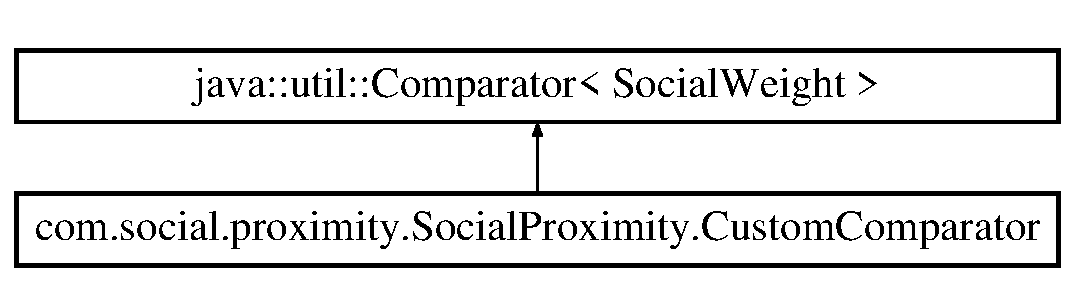
\includegraphics[height=2.000000cm]{classcom_1_1social_1_1proximity_1_1_social_proximity_1_1_custom_comparator}
\end{center}
\end{figure}
\subsection*{Public Member Functions}
\begin{DoxyCompactItemize}
\item 
int \hyperlink{classcom_1_1social_1_1proximity_1_1_social_proximity_1_1_custom_comparator_a7546b43a5c67840f91cf5f6e1b433725}{compare} (\hyperlink{classcom_1_1social_1_1proximity_1_1_social_weight}{Social\+Weight} entry1, \hyperlink{classcom_1_1social_1_1proximity_1_1_social_weight}{Social\+Weight} entry2)
\end{DoxyCompactItemize}


\subsection{Member Function Documentation}
\hypertarget{classcom_1_1social_1_1proximity_1_1_social_proximity_1_1_custom_comparator_a7546b43a5c67840f91cf5f6e1b433725}{}\index{com\+::social\+::proximity\+::\+Social\+Proximity\+::\+Custom\+Comparator@{com\+::social\+::proximity\+::\+Social\+Proximity\+::\+Custom\+Comparator}!compare@{compare}}
\index{compare@{compare}!com\+::social\+::proximity\+::\+Social\+Proximity\+::\+Custom\+Comparator@{com\+::social\+::proximity\+::\+Social\+Proximity\+::\+Custom\+Comparator}}
\subsubsection[{compare(\+Social\+Weight entry1, Social\+Weight entry2)}]{\setlength{\rightskip}{0pt plus 5cm}int com.\+social.\+proximity.\+Social\+Proximity.\+Custom\+Comparator.\+compare (
\begin{DoxyParamCaption}
\item[{{\bf Social\+Weight}}]{entry1, }
\item[{{\bf Social\+Weight}}]{entry2}
\end{DoxyParamCaption}
)}\label{classcom_1_1social_1_1proximity_1_1_social_proximity_1_1_custom_comparator_a7546b43a5c67840f91cf5f6e1b433725}


The documentation for this class was generated from the following file\+:\begin{DoxyCompactItemize}
\item 
src/com/social/proximity/\hyperlink{_social_proximity_8java}{Social\+Proximity.\+java}\end{DoxyCompactItemize}

\hypertarget{interfacecom_1_1social_1_1proximity_1_1_data_base_change_listener}{}\section{com.\+social.\+proximity.\+Data\+Base\+Change\+Listener Interface Reference}
\label{interfacecom_1_1social_1_1proximity_1_1_data_base_change_listener}\index{com.\+social.\+proximity.\+Data\+Base\+Change\+Listener@{com.\+social.\+proximity.\+Data\+Base\+Change\+Listener}}
\subsection*{Public Member Functions}
\begin{DoxyCompactItemize}
\item 
void \hyperlink{interfacecom_1_1social_1_1proximity_1_1_data_base_change_listener_ac8064dca0d90e804d6943c51a4464b2e}{on\+Data\+Base\+Change\+B\+T} (Array\+List$<$ \hyperlink{classcom_1_1social_1_1proximity_1_1_b_t_user_device}{B\+T\+User\+Device} $>$ array\+List)
\item 
void \hyperlink{interfacecom_1_1social_1_1proximity_1_1_data_base_change_listener_ae0bb6bcc342acb5d16c605ba959ad23c}{on\+Data\+Base\+Change\+B\+T\+Enc\+Dur} (Array\+List$<$ \hyperlink{classcom_1_1social_1_1proximity_1_1_b_t_user_dev_encounter_duration}{B\+T\+User\+Dev\+Encounter\+Duration} $>$ array\+List)
\item 
void \hyperlink{interfacecom_1_1social_1_1proximity_1_1_data_base_change_listener_a2a071c7aabce3cdbc1b1f5d0c5e0fb24}{on\+Data\+Base\+Change\+B\+T\+Avg\+Enc\+Dur} (Array\+List$<$ \hyperlink{classcom_1_1social_1_1proximity_1_1_b_t_user_dev_average_encounter_duration}{B\+T\+User\+Dev\+Average\+Encounter\+Duration} $>$ array\+List)
\item 
void \hyperlink{interfacecom_1_1social_1_1proximity_1_1_data_base_change_listener_abd4716358cbfbd0ba1cef920ae5a4bf1}{on\+Data\+Base\+Change\+B\+T\+Social\+Weight} (Array\+List$<$ \hyperlink{classcom_1_1social_1_1proximity_1_1_b_t_user_dev_social_weight}{B\+T\+User\+Dev\+Social\+Weight} $>$ array\+List)
\end{DoxyCompactItemize}


\subsection{Member Function Documentation}
\hypertarget{interfacecom_1_1social_1_1proximity_1_1_data_base_change_listener_ac8064dca0d90e804d6943c51a4464b2e}{}\index{com\+::social\+::proximity\+::\+Data\+Base\+Change\+Listener@{com\+::social\+::proximity\+::\+Data\+Base\+Change\+Listener}!on\+Data\+Base\+Change\+B\+T@{on\+Data\+Base\+Change\+B\+T}}
\index{on\+Data\+Base\+Change\+B\+T@{on\+Data\+Base\+Change\+B\+T}!com\+::social\+::proximity\+::\+Data\+Base\+Change\+Listener@{com\+::social\+::proximity\+::\+Data\+Base\+Change\+Listener}}
\subsubsection[{on\+Data\+Base\+Change\+B\+T(\+Array\+List$<$ B\+T\+User\+Device $>$ array\+List)}]{\setlength{\rightskip}{0pt plus 5cm}void com.\+social.\+proximity.\+Data\+Base\+Change\+Listener.\+on\+Data\+Base\+Change\+B\+T (
\begin{DoxyParamCaption}
\item[{Array\+List$<$ {\bf B\+T\+User\+Device} $>$}]{array\+List}
\end{DoxyParamCaption}
)}\label{interfacecom_1_1social_1_1proximity_1_1_data_base_change_listener_ac8064dca0d90e804d6943c51a4464b2e}
Reports on changes on the Bluetooth device information. 
\begin{DoxyParams}{Parameters}
{\em array\+List} & The list containing the peer information (M\+A\+C address, device\textquotesingle{}s name, and time of first encounter). \\
\hline
\end{DoxyParams}
\hypertarget{interfacecom_1_1social_1_1proximity_1_1_data_base_change_listener_a2a071c7aabce3cdbc1b1f5d0c5e0fb24}{}\index{com\+::social\+::proximity\+::\+Data\+Base\+Change\+Listener@{com\+::social\+::proximity\+::\+Data\+Base\+Change\+Listener}!on\+Data\+Base\+Change\+B\+T\+Avg\+Enc\+Dur@{on\+Data\+Base\+Change\+B\+T\+Avg\+Enc\+Dur}}
\index{on\+Data\+Base\+Change\+B\+T\+Avg\+Enc\+Dur@{on\+Data\+Base\+Change\+B\+T\+Avg\+Enc\+Dur}!com\+::social\+::proximity\+::\+Data\+Base\+Change\+Listener@{com\+::social\+::proximity\+::\+Data\+Base\+Change\+Listener}}
\subsubsection[{on\+Data\+Base\+Change\+B\+T\+Avg\+Enc\+Dur(\+Array\+List$<$ B\+T\+User\+Dev\+Average\+Encounter\+Duration $>$ array\+List)}]{\setlength{\rightskip}{0pt plus 5cm}void com.\+social.\+proximity.\+Data\+Base\+Change\+Listener.\+on\+Data\+Base\+Change\+B\+T\+Avg\+Enc\+Dur (
\begin{DoxyParamCaption}
\item[{Array\+List$<$ {\bf B\+T\+User\+Dev\+Average\+Encounter\+Duration} $>$}]{array\+List}
\end{DoxyParamCaption}
)}\label{interfacecom_1_1social_1_1proximity_1_1_data_base_change_listener_a2a071c7aabce3cdbc1b1f5d0c5e0fb24}
Reports on changes on the Bluetooth device information. 
\begin{DoxyParams}{Parameters}
{\em array\+List} & The list containing the peer information (M\+A\+C address and average encounter duration). \\
\hline
\end{DoxyParams}
\hypertarget{interfacecom_1_1social_1_1proximity_1_1_data_base_change_listener_ae0bb6bcc342acb5d16c605ba959ad23c}{}\index{com\+::social\+::proximity\+::\+Data\+Base\+Change\+Listener@{com\+::social\+::proximity\+::\+Data\+Base\+Change\+Listener}!on\+Data\+Base\+Change\+B\+T\+Enc\+Dur@{on\+Data\+Base\+Change\+B\+T\+Enc\+Dur}}
\index{on\+Data\+Base\+Change\+B\+T\+Enc\+Dur@{on\+Data\+Base\+Change\+B\+T\+Enc\+Dur}!com\+::social\+::proximity\+::\+Data\+Base\+Change\+Listener@{com\+::social\+::proximity\+::\+Data\+Base\+Change\+Listener}}
\subsubsection[{on\+Data\+Base\+Change\+B\+T\+Enc\+Dur(\+Array\+List$<$ B\+T\+User\+Dev\+Encounter\+Duration $>$ array\+List)}]{\setlength{\rightskip}{0pt plus 5cm}void com.\+social.\+proximity.\+Data\+Base\+Change\+Listener.\+on\+Data\+Base\+Change\+B\+T\+Enc\+Dur (
\begin{DoxyParamCaption}
\item[{Array\+List$<$ {\bf B\+T\+User\+Dev\+Encounter\+Duration} $>$}]{array\+List}
\end{DoxyParamCaption}
)}\label{interfacecom_1_1social_1_1proximity_1_1_data_base_change_listener_ae0bb6bcc342acb5d16c605ba959ad23c}
Reports on changes on the Bluetooth device information. 
\begin{DoxyParams}{Parameters}
{\em array\+List} & The list containing the peer information (M\+A\+C address and time spent in the vicinity, i.\+e., total time within communication range). \\
\hline
\end{DoxyParams}
\hypertarget{interfacecom_1_1social_1_1proximity_1_1_data_base_change_listener_abd4716358cbfbd0ba1cef920ae5a4bf1}{}\index{com\+::social\+::proximity\+::\+Data\+Base\+Change\+Listener@{com\+::social\+::proximity\+::\+Data\+Base\+Change\+Listener}!on\+Data\+Base\+Change\+B\+T\+Social\+Weight@{on\+Data\+Base\+Change\+B\+T\+Social\+Weight}}
\index{on\+Data\+Base\+Change\+B\+T\+Social\+Weight@{on\+Data\+Base\+Change\+B\+T\+Social\+Weight}!com\+::social\+::proximity\+::\+Data\+Base\+Change\+Listener@{com\+::social\+::proximity\+::\+Data\+Base\+Change\+Listener}}
\subsubsection[{on\+Data\+Base\+Change\+B\+T\+Social\+Weight(\+Array\+List$<$ B\+T\+User\+Dev\+Social\+Weight $>$ array\+List)}]{\setlength{\rightskip}{0pt plus 5cm}void com.\+social.\+proximity.\+Data\+Base\+Change\+Listener.\+on\+Data\+Base\+Change\+B\+T\+Social\+Weight (
\begin{DoxyParamCaption}
\item[{Array\+List$<$ {\bf B\+T\+User\+Dev\+Social\+Weight} $>$}]{array\+List}
\end{DoxyParamCaption}
)}\label{interfacecom_1_1social_1_1proximity_1_1_data_base_change_listener_abd4716358cbfbd0ba1cef920ae5a4bf1}
Reports on changes on the Bluetooth device information. 
\begin{DoxyParams}{Parameters}
{\em array\+List} & The list containing the peer information (M\+A\+C address and social weight). \\
\hline
\end{DoxyParams}


The documentation for this interface was generated from the following file\+:\begin{DoxyCompactItemize}
\item 
src/com/social/proximity/\hyperlink{_data_base_change_listener_8java}{Data\+Base\+Change\+Listener.\+java}\end{DoxyCompactItemize}

\hypertarget{classcom_1_1social_1_1proximity_1_1_database_functions}{}\section{com.\+social.\+proximity.\+Database\+Functions Class Reference}
\label{classcom_1_1social_1_1proximity_1_1_database_functions}\index{com.\+social.\+proximity.\+Database\+Functions@{com.\+social.\+proximity.\+Database\+Functions}}
\subsection*{Public Member Functions}
\begin{DoxyCompactItemize}
\item 
\hyperlink{classcom_1_1social_1_1proximity_1_1_database_functions_ad9923ea46c9cad358faf955ec624361e}{Database\+Functions} (S\+Q\+Lite\+Database database)
\item 
long \hyperlink{classcom_1_1social_1_1proximity_1_1_database_functions_a2e880b0dafb20139937f18a5e90b3649}{get\+Num\+B\+T\+Device} ()
\item 
void \hyperlink{classcom_1_1social_1_1proximity_1_1_database_functions_a525dc9e96941587a650435b01b1e14b2}{register\+New\+B\+T\+Device} (\hyperlink{classcom_1_1social_1_1proximity_1_1_b_t_user_device}{B\+T\+User\+Device} bt\+Dev, \hyperlink{classcom_1_1social_1_1proximity_1_1_b_t_user_dev_encounter_duration}{B\+T\+User\+Dev\+Encounter\+Duration} duration, \hyperlink{classcom_1_1social_1_1proximity_1_1_b_t_user_dev_average_encounter_duration}{B\+T\+User\+Dev\+Average\+Encounter\+Duration} average\+Duration, \hyperlink{classcom_1_1social_1_1proximity_1_1_b_t_user_dev_social_weight}{B\+T\+User\+Dev\+Social\+Weight} social\+Weight)
\item 
void \hyperlink{classcom_1_1social_1_1proximity_1_1_database_functions_afa77844cfc5644e5daae5ad713d2c11c}{update\+B\+T\+Device\+And\+Duration} (\hyperlink{classcom_1_1social_1_1proximity_1_1_b_t_user_device}{B\+T\+User\+Device} bt\+Dev, \hyperlink{classcom_1_1social_1_1proximity_1_1_b_t_user_dev_encounter_duration}{B\+T\+User\+Dev\+Encounter\+Duration} duration)
\item 
void \hyperlink{classcom_1_1social_1_1proximity_1_1_database_functions_a2ab63e9a49b88ef8549905b50c26e8e7}{update\+B\+T\+Dev\+Avg\+Encounter\+Duration} (\hyperlink{classcom_1_1social_1_1proximity_1_1_b_t_user_dev_average_encounter_duration}{B\+T\+User\+Dev\+Average\+Encounter\+Duration} average\+Duration)
\item 
void \hyperlink{classcom_1_1social_1_1proximity_1_1_database_functions_abba6ca6e0149bfc752fe40748328611b}{update\+B\+T\+Dev\+Social\+Weight} (\hyperlink{classcom_1_1social_1_1proximity_1_1_b_t_user_dev_social_weight}{B\+T\+User\+Dev\+Social\+Weight} social\+Weight)
\item 
\hyperlink{classcom_1_1social_1_1proximity_1_1_b_t_user_device}{B\+T\+User\+Device} \hyperlink{classcom_1_1social_1_1proximity_1_1_database_functions_acb105b2d152bebca021902a532023f8a}{get\+B\+T\+Device} (String bt\+Device)
\item 
\hyperlink{classcom_1_1social_1_1proximity_1_1_b_t_user_dev_encounter_duration}{B\+T\+User\+Dev\+Encounter\+Duration} \hyperlink{classcom_1_1social_1_1proximity_1_1_database_functions_ac1abea0c449b91b3a7cef0d435dd380d}{get\+B\+T\+Device\+Encounter\+Duration} (String bt\+Dev\+Encounter\+Duration)
\item 
\hyperlink{classcom_1_1social_1_1proximity_1_1_b_t_user_dev_average_encounter_duration}{B\+T\+User\+Dev\+Average\+Encounter\+Duration} \hyperlink{classcom_1_1social_1_1proximity_1_1_database_functions_a1560c9dea6ddc6d0723bc94dcf239d88}{get\+B\+T\+Device\+Average\+Encounter\+Duration} (String bt\+Dev\+Average\+Encounter\+Duration)
\item 
\hyperlink{classcom_1_1social_1_1proximity_1_1_b_t_user_dev_social_weight}{B\+T\+User\+Dev\+Social\+Weight} \hyperlink{classcom_1_1social_1_1proximity_1_1_database_functions_aec10373c2ee3c4cbb74df29e1bfd3ba4}{get\+B\+T\+Device\+Social\+Weight} (String bt\+Dev\+Social\+Weight)
\item 
boolean \hyperlink{classcom_1_1social_1_1proximity_1_1_database_functions_a79227cf1e1fccd36b772389bf41bc84c}{has\+B\+T\+Device} (String bt\+Dev)
\item 
Map$<$ String, \hyperlink{classcom_1_1social_1_1proximity_1_1_b_t_user_device}{B\+T\+User\+Device} $>$ \hyperlink{classcom_1_1social_1_1proximity_1_1_database_functions_a4e1682f27d7730266f9b2a7a8fc49973}{get\+All\+B\+T\+Device} ()
\item 
Map$<$ String, \hyperlink{classcom_1_1social_1_1proximity_1_1_b_t_user_dev_encounter_duration}{B\+T\+User\+Dev\+Encounter\+Duration} $>$ \hyperlink{classcom_1_1social_1_1proximity_1_1_database_functions_af6d76fcca3b7f7d3e28e6f576a68d17b}{get\+All\+B\+T\+Dev\+Encounter\+Duration} ()
\item 
Map$<$ String, \hyperlink{classcom_1_1social_1_1proximity_1_1_b_t_user_dev_average_encounter_duration}{B\+T\+User\+Dev\+Average\+Encounter\+Duration} $>$ \hyperlink{classcom_1_1social_1_1proximity_1_1_database_functions_a48db6e5dea3fd9f5b14ceaa06bc94e53}{get\+All\+B\+T\+Dev\+Average\+Encounter\+Duration} ()
\item 
Map$<$ String, \hyperlink{classcom_1_1social_1_1proximity_1_1_b_t_user_dev_social_weight}{B\+T\+User\+Dev\+Social\+Weight} $>$ \hyperlink{classcom_1_1social_1_1proximity_1_1_database_functions_a44836cb8d594ac50db08048f50915af8}{get\+All\+B\+T\+Dev\+Social\+Weight} ()
\end{DoxyCompactItemize}
\subsection*{Private Member Functions}
\begin{DoxyCompactItemize}
\item 
\hyperlink{classcom_1_1social_1_1proximity_1_1_b_t_user_device}{B\+T\+User\+Device} \hyperlink{classcom_1_1social_1_1proximity_1_1_database_functions_a8d5062709948e54d224ac1b65637e4fc}{cursor\+To\+B\+T\+Device} (Cursor cursor)
\item 
\hyperlink{classcom_1_1social_1_1proximity_1_1_b_t_user_dev_encounter_duration}{B\+T\+User\+Dev\+Encounter\+Duration} \hyperlink{classcom_1_1social_1_1proximity_1_1_database_functions_a405dbb37f14ca70e94b8ecad32d323f1}{cursor\+To\+B\+T\+Dev\+Encounter\+Duration} (Cursor cursor)
\item 
\hyperlink{classcom_1_1social_1_1proximity_1_1_b_t_user_dev_average_encounter_duration}{B\+T\+User\+Dev\+Average\+Encounter\+Duration} \hyperlink{classcom_1_1social_1_1proximity_1_1_database_functions_a80ba14678e2170e8798f1412fccec08a}{cursor\+To\+B\+T\+Dev\+Average\+Encounter\+Duration} (Cursor cursor)
\item 
\hyperlink{classcom_1_1social_1_1proximity_1_1_b_t_user_dev_social_weight}{B\+T\+User\+Dev\+Social\+Weight} \hyperlink{classcom_1_1social_1_1proximity_1_1_database_functions_ab76111ebce8e97043be7975514a8dec4}{cursor\+To\+B\+T\+Dev\+Social\+Weight} (Cursor cursor)
\end{DoxyCompactItemize}
\subsection*{Private Attributes}
\begin{DoxyCompactItemize}
\item 
S\+Q\+Lite\+Database \hyperlink{classcom_1_1social_1_1proximity_1_1_database_functions_a6b12c0a8d4be24df06fbc5117840e2e1}{db}
\item 
String\mbox{[}$\,$\mbox{]} \hyperlink{classcom_1_1social_1_1proximity_1_1_database_functions_a83354aec2042f330c23bde5edf553129}{all\+Columns\+B\+T\+Devices}
\item 
String\mbox{[}$\,$\mbox{]} \hyperlink{classcom_1_1social_1_1proximity_1_1_database_functions_ab59f771fe031574737a9c5a9487d2540}{all\+Columns\+B\+T\+Device\+Encounter\+Duration}
\item 
String\mbox{[}$\,$\mbox{]} \hyperlink{classcom_1_1social_1_1proximity_1_1_database_functions_a37740a5005b0a87d33dc3f25f7433474}{all\+Columns\+B\+T\+Device\+Average\+Encounter\+Duration}
\item 
String\mbox{[}$\,$\mbox{]} \hyperlink{classcom_1_1social_1_1proximity_1_1_database_functions_a5cb0795326bc5712e498557e68a2f3e7}{all\+Columns\+B\+T\+Device\+Social\+Weight}
\end{DoxyCompactItemize}


\subsection{Constructor \& Destructor Documentation}
\hypertarget{classcom_1_1social_1_1proximity_1_1_database_functions_ad9923ea46c9cad358faf955ec624361e}{}\index{com\+::social\+::proximity\+::\+Database\+Functions@{com\+::social\+::proximity\+::\+Database\+Functions}!Database\+Functions@{Database\+Functions}}
\index{Database\+Functions@{Database\+Functions}!com\+::social\+::proximity\+::\+Database\+Functions@{com\+::social\+::proximity\+::\+Database\+Functions}}
\subsubsection[{Database\+Functions(\+S\+Q\+Lite\+Database database)}]{\setlength{\rightskip}{0pt plus 5cm}com.\+social.\+proximity.\+Database\+Functions.\+Database\+Functions (
\begin{DoxyParamCaption}
\item[{S\+Q\+Lite\+Database}]{database}
\end{DoxyParamCaption}
)}\label{classcom_1_1social_1_1proximity_1_1_database_functions_ad9923ea46c9cad358faf955ec624361e}
\hyperlink{classcom_1_1social_1_1proximity_1_1_database_functions}{Database\+Functions} constructor. 
\begin{DoxyParams}{Parameters}
{\em database} & The database provided by the application. \\
\hline
\end{DoxyParams}


\subsection{Member Function Documentation}
\hypertarget{classcom_1_1social_1_1proximity_1_1_database_functions_a80ba14678e2170e8798f1412fccec08a}{}\index{com\+::social\+::proximity\+::\+Database\+Functions@{com\+::social\+::proximity\+::\+Database\+Functions}!cursor\+To\+B\+T\+Dev\+Average\+Encounter\+Duration@{cursor\+To\+B\+T\+Dev\+Average\+Encounter\+Duration}}
\index{cursor\+To\+B\+T\+Dev\+Average\+Encounter\+Duration@{cursor\+To\+B\+T\+Dev\+Average\+Encounter\+Duration}!com\+::social\+::proximity\+::\+Database\+Functions@{com\+::social\+::proximity\+::\+Database\+Functions}}
\subsubsection[{cursor\+To\+B\+T\+Dev\+Average\+Encounter\+Duration(\+Cursor cursor)}]{\setlength{\rightskip}{0pt plus 5cm}{\bf B\+T\+User\+Dev\+Average\+Encounter\+Duration} com.\+social.\+proximity.\+Database\+Functions.\+cursor\+To\+B\+T\+Dev\+Average\+Encounter\+Duration (
\begin{DoxyParamCaption}
\item[{Cursor}]{cursor}
\end{DoxyParamCaption}
)\hspace{0.3cm}{\ttfamily [private]}}\label{classcom_1_1social_1_1proximity_1_1_database_functions_a80ba14678e2170e8798f1412fccec08a}
Converts a cursor pointing to a record in the B\+T\+D\+E\+V\+I\+C\+E\+A\+V\+E\+R\+A\+G\+E\+E\+N\+C\+O\+U\+N\+T\+E\+R\+D\+U\+R\+A\+T\+I\+O\+N table to a \hyperlink{classcom_1_1social_1_1proximity_1_1_b_t_user_dev_average_encounter_duration}{B\+T\+User\+Dev\+Average\+Encounter\+Duration} object. 
\begin{DoxyParams}{Parameters}
{\em cursor} & Cursor pointing to a record of the B\+T\+D\+E\+V\+I\+C\+E\+A\+V\+E\+R\+A\+G\+E\+E\+N\+C\+O\+U\+N\+T\+E\+R\+D\+U\+R\+A\+T\+I\+O\+N table. \\
\hline
\end{DoxyParams}
\begin{DoxyReturn}{Returns}
the \hyperlink{classcom_1_1social_1_1proximity_1_1_b_t_user_dev_average_encounter_duration}{B\+T\+User\+Dev\+Average\+Encounter\+Duration} object. 
\end{DoxyReturn}
\hypertarget{classcom_1_1social_1_1proximity_1_1_database_functions_a405dbb37f14ca70e94b8ecad32d323f1}{}\index{com\+::social\+::proximity\+::\+Database\+Functions@{com\+::social\+::proximity\+::\+Database\+Functions}!cursor\+To\+B\+T\+Dev\+Encounter\+Duration@{cursor\+To\+B\+T\+Dev\+Encounter\+Duration}}
\index{cursor\+To\+B\+T\+Dev\+Encounter\+Duration@{cursor\+To\+B\+T\+Dev\+Encounter\+Duration}!com\+::social\+::proximity\+::\+Database\+Functions@{com\+::social\+::proximity\+::\+Database\+Functions}}
\subsubsection[{cursor\+To\+B\+T\+Dev\+Encounter\+Duration(\+Cursor cursor)}]{\setlength{\rightskip}{0pt plus 5cm}{\bf B\+T\+User\+Dev\+Encounter\+Duration} com.\+social.\+proximity.\+Database\+Functions.\+cursor\+To\+B\+T\+Dev\+Encounter\+Duration (
\begin{DoxyParamCaption}
\item[{Cursor}]{cursor}
\end{DoxyParamCaption}
)\hspace{0.3cm}{\ttfamily [private]}}\label{classcom_1_1social_1_1proximity_1_1_database_functions_a405dbb37f14ca70e94b8ecad32d323f1}
Converts a cursor pointing to a record in the B\+T\+D\+E\+V\+I\+C\+E\+E\+N\+C\+O\+U\+N\+T\+E\+R\+D\+U\+R\+A\+T\+I\+O\+N table to a \hyperlink{classcom_1_1social_1_1proximity_1_1_b_t_user_dev_encounter_duration}{B\+T\+User\+Dev\+Encounter\+Duration} object. 
\begin{DoxyParams}{Parameters}
{\em cursor} & Cursor pointing to a record of the B\+T\+D\+E\+V\+I\+C\+E\+E\+N\+C\+O\+U\+N\+T\+E\+R\+D\+U\+R\+A\+T\+I\+O\+N table. \\
\hline
\end{DoxyParams}
\begin{DoxyReturn}{Returns}
the \hyperlink{classcom_1_1social_1_1proximity_1_1_b_t_user_dev_encounter_duration}{B\+T\+User\+Dev\+Encounter\+Duration} object. 
\end{DoxyReturn}
\hypertarget{classcom_1_1social_1_1proximity_1_1_database_functions_a8d5062709948e54d224ac1b65637e4fc}{}\index{com\+::social\+::proximity\+::\+Database\+Functions@{com\+::social\+::proximity\+::\+Database\+Functions}!cursor\+To\+B\+T\+Device@{cursor\+To\+B\+T\+Device}}
\index{cursor\+To\+B\+T\+Device@{cursor\+To\+B\+T\+Device}!com\+::social\+::proximity\+::\+Database\+Functions@{com\+::social\+::proximity\+::\+Database\+Functions}}
\subsubsection[{cursor\+To\+B\+T\+Device(\+Cursor cursor)}]{\setlength{\rightskip}{0pt plus 5cm}{\bf B\+T\+User\+Device} com.\+social.\+proximity.\+Database\+Functions.\+cursor\+To\+B\+T\+Device (
\begin{DoxyParamCaption}
\item[{Cursor}]{cursor}
\end{DoxyParamCaption}
)\hspace{0.3cm}{\ttfamily [private]}}\label{classcom_1_1social_1_1proximity_1_1_database_functions_a8d5062709948e54d224ac1b65637e4fc}
Converts a cursor pointing to a record in the B\+T\+D\+E\+V\+I\+C\+E table to a B\+T\+Device object. 
\begin{DoxyParams}{Parameters}
{\em cursor} & Cursor pointing to a record of the B\+T\+D\+E\+V\+I\+C\+E table. \\
\hline
\end{DoxyParams}
\begin{DoxyReturn}{Returns}
the B\+T\+Device object. 
\end{DoxyReturn}
\hypertarget{classcom_1_1social_1_1proximity_1_1_database_functions_ab76111ebce8e97043be7975514a8dec4}{}\index{com\+::social\+::proximity\+::\+Database\+Functions@{com\+::social\+::proximity\+::\+Database\+Functions}!cursor\+To\+B\+T\+Dev\+Social\+Weight@{cursor\+To\+B\+T\+Dev\+Social\+Weight}}
\index{cursor\+To\+B\+T\+Dev\+Social\+Weight@{cursor\+To\+B\+T\+Dev\+Social\+Weight}!com\+::social\+::proximity\+::\+Database\+Functions@{com\+::social\+::proximity\+::\+Database\+Functions}}
\subsubsection[{cursor\+To\+B\+T\+Dev\+Social\+Weight(\+Cursor cursor)}]{\setlength{\rightskip}{0pt plus 5cm}{\bf B\+T\+User\+Dev\+Social\+Weight} com.\+social.\+proximity.\+Database\+Functions.\+cursor\+To\+B\+T\+Dev\+Social\+Weight (
\begin{DoxyParamCaption}
\item[{Cursor}]{cursor}
\end{DoxyParamCaption}
)\hspace{0.3cm}{\ttfamily [private]}}\label{classcom_1_1social_1_1proximity_1_1_database_functions_ab76111ebce8e97043be7975514a8dec4}
Converts a cursor pointing to a record in the B\+T\+D\+E\+V\+I\+C\+E\+S\+O\+C\+I\+A\+L\+W\+E\+I\+G\+H\+T table to a \hyperlink{classcom_1_1social_1_1proximity_1_1_b_t_user_dev_social_weight}{B\+T\+User\+Dev\+Social\+Weight} object. 
\begin{DoxyParams}{Parameters}
{\em cursor} & Cursor pointing to a record of the B\+T\+D\+E\+V\+I\+C\+E\+A\+V\+E\+R\+A\+G\+E\+E\+N\+C\+O\+U\+N\+T\+E\+R\+D\+U\+R\+A\+T\+I\+O\+N table. \\
\hline
\end{DoxyParams}
\begin{DoxyReturn}{Returns}
the \hyperlink{classcom_1_1social_1_1proximity_1_1_b_t_user_dev_social_weight}{B\+T\+User\+Dev\+Social\+Weight} object. 
\end{DoxyReturn}
\hypertarget{classcom_1_1social_1_1proximity_1_1_database_functions_a48db6e5dea3fd9f5b14ceaa06bc94e53}{}\index{com\+::social\+::proximity\+::\+Database\+Functions@{com\+::social\+::proximity\+::\+Database\+Functions}!get\+All\+B\+T\+Dev\+Average\+Encounter\+Duration@{get\+All\+B\+T\+Dev\+Average\+Encounter\+Duration}}
\index{get\+All\+B\+T\+Dev\+Average\+Encounter\+Duration@{get\+All\+B\+T\+Dev\+Average\+Encounter\+Duration}!com\+::social\+::proximity\+::\+Database\+Functions@{com\+::social\+::proximity\+::\+Database\+Functions}}
\subsubsection[{get\+All\+B\+T\+Dev\+Average\+Encounter\+Duration()}]{\setlength{\rightskip}{0pt plus 5cm}Map$<$String, {\bf B\+T\+User\+Dev\+Average\+Encounter\+Duration}$>$ com.\+social.\+proximity.\+Database\+Functions.\+get\+All\+B\+T\+Dev\+Average\+Encounter\+Duration (
\begin{DoxyParamCaption}
{}
\end{DoxyParamCaption}
)}\label{classcom_1_1social_1_1proximity_1_1_database_functions_a48db6e5dea3fd9f5b14ceaa06bc94e53}
Gets the all the \hyperlink{classcom_1_1social_1_1proximity_1_1_b_t_user_dev_average_encounter_duration}{B\+T\+User\+Dev\+Average\+Encounter\+Duration} recorded by the application on the B\+T\+D\+E\+V\+I\+C\+E\+A\+V\+E\+R\+A\+G\+E\+E\+N\+C\+O\+U\+N\+T\+E\+R\+D\+U\+R\+A\+T\+I\+O\+N table. \begin{DoxyReturn}{Returns}
bt\+Dev\+Average\+Encounter\+Duration\+Map A map with the \hyperlink{classcom_1_1social_1_1proximity_1_1_b_t_user_dev_average_encounter_duration}{B\+T\+User\+Dev\+Average\+Encounter\+Duration} objects, and the B\+T\+D\+E\+V\+\_\+\+M\+A\+C\+\_\+\+A\+D\+D\+R\+E\+S\+S as key. 
\end{DoxyReturn}
\hypertarget{classcom_1_1social_1_1proximity_1_1_database_functions_af6d76fcca3b7f7d3e28e6f576a68d17b}{}\index{com\+::social\+::proximity\+::\+Database\+Functions@{com\+::social\+::proximity\+::\+Database\+Functions}!get\+All\+B\+T\+Dev\+Encounter\+Duration@{get\+All\+B\+T\+Dev\+Encounter\+Duration}}
\index{get\+All\+B\+T\+Dev\+Encounter\+Duration@{get\+All\+B\+T\+Dev\+Encounter\+Duration}!com\+::social\+::proximity\+::\+Database\+Functions@{com\+::social\+::proximity\+::\+Database\+Functions}}
\subsubsection[{get\+All\+B\+T\+Dev\+Encounter\+Duration()}]{\setlength{\rightskip}{0pt plus 5cm}Map$<$String, {\bf B\+T\+User\+Dev\+Encounter\+Duration}$>$ com.\+social.\+proximity.\+Database\+Functions.\+get\+All\+B\+T\+Dev\+Encounter\+Duration (
\begin{DoxyParamCaption}
{}
\end{DoxyParamCaption}
)}\label{classcom_1_1social_1_1proximity_1_1_database_functions_af6d76fcca3b7f7d3e28e6f576a68d17b}
Gets the all the \hyperlink{classcom_1_1social_1_1proximity_1_1_b_t_user_dev_encounter_duration}{B\+T\+User\+Dev\+Encounter\+Duration} recorded by the application on the B\+T\+D\+E\+V\+I\+C\+E\+E\+N\+C\+O\+U\+N\+T\+E\+R\+D\+U\+R\+A\+T\+I\+O\+N table. \begin{DoxyReturn}{Returns}
bt\+Dev\+Encounter\+Duration\+Map A map with the \hyperlink{classcom_1_1social_1_1proximity_1_1_b_t_user_dev_encounter_duration}{B\+T\+User\+Dev\+Encounter\+Duration} objects, and the B\+T\+D\+E\+V\+\_\+\+M\+A\+C\+\_\+\+A\+D\+D\+R\+E\+S\+S as key. 
\end{DoxyReturn}
\hypertarget{classcom_1_1social_1_1proximity_1_1_database_functions_a4e1682f27d7730266f9b2a7a8fc49973}{}\index{com\+::social\+::proximity\+::\+Database\+Functions@{com\+::social\+::proximity\+::\+Database\+Functions}!get\+All\+B\+T\+Device@{get\+All\+B\+T\+Device}}
\index{get\+All\+B\+T\+Device@{get\+All\+B\+T\+Device}!com\+::social\+::proximity\+::\+Database\+Functions@{com\+::social\+::proximity\+::\+Database\+Functions}}
\subsubsection[{get\+All\+B\+T\+Device()}]{\setlength{\rightskip}{0pt plus 5cm}Map$<$String, {\bf B\+T\+User\+Device}$>$ com.\+social.\+proximity.\+Database\+Functions.\+get\+All\+B\+T\+Device (
\begin{DoxyParamCaption}
{}
\end{DoxyParamCaption}
)}\label{classcom_1_1social_1_1proximity_1_1_database_functions_a4e1682f27d7730266f9b2a7a8fc49973}
Gets the all the B\+T\+Device recorded by the application on the B\+T\+D\+E\+V\+I\+C\+E table. \begin{DoxyReturn}{Returns}
bt\+Dev\+Map A map with the \hyperlink{classcom_1_1social_1_1proximity_1_1_b_t_user_device}{B\+T\+User\+Device} objects, and the B\+T\+D\+E\+V\+\_\+\+M\+A\+C\+\_\+\+A\+D\+D\+R\+E\+S\+S as key. 
\end{DoxyReturn}
\hypertarget{classcom_1_1social_1_1proximity_1_1_database_functions_a44836cb8d594ac50db08048f50915af8}{}\index{com\+::social\+::proximity\+::\+Database\+Functions@{com\+::social\+::proximity\+::\+Database\+Functions}!get\+All\+B\+T\+Dev\+Social\+Weight@{get\+All\+B\+T\+Dev\+Social\+Weight}}
\index{get\+All\+B\+T\+Dev\+Social\+Weight@{get\+All\+B\+T\+Dev\+Social\+Weight}!com\+::social\+::proximity\+::\+Database\+Functions@{com\+::social\+::proximity\+::\+Database\+Functions}}
\subsubsection[{get\+All\+B\+T\+Dev\+Social\+Weight()}]{\setlength{\rightskip}{0pt plus 5cm}Map$<$String, {\bf B\+T\+User\+Dev\+Social\+Weight}$>$ com.\+social.\+proximity.\+Database\+Functions.\+get\+All\+B\+T\+Dev\+Social\+Weight (
\begin{DoxyParamCaption}
{}
\end{DoxyParamCaption}
)}\label{classcom_1_1social_1_1proximity_1_1_database_functions_a44836cb8d594ac50db08048f50915af8}
Gets the all the \hyperlink{classcom_1_1social_1_1proximity_1_1_b_t_user_dev_social_weight}{B\+T\+User\+Dev\+Social\+Weight} recorded by the application on the B\+T\+D\+E\+V\+I\+C\+E\+S\+O\+C\+I\+A\+L\+W\+E\+I\+G\+H\+T table. \begin{DoxyReturn}{Returns}
bt\+Dev\+Social\+Weight\+Map A map with the \hyperlink{classcom_1_1social_1_1proximity_1_1_b_t_user_dev_social_weight}{B\+T\+User\+Dev\+Social\+Weight} objects, and the B\+T\+D\+E\+V\+\_\+\+M\+A\+C\+\_\+\+A\+D\+D\+R\+E\+S\+S as key. 
\end{DoxyReturn}
\hypertarget{classcom_1_1social_1_1proximity_1_1_database_functions_acb105b2d152bebca021902a532023f8a}{}\index{com\+::social\+::proximity\+::\+Database\+Functions@{com\+::social\+::proximity\+::\+Database\+Functions}!get\+B\+T\+Device@{get\+B\+T\+Device}}
\index{get\+B\+T\+Device@{get\+B\+T\+Device}!com\+::social\+::proximity\+::\+Database\+Functions@{com\+::social\+::proximity\+::\+Database\+Functions}}
\subsubsection[{get\+B\+T\+Device(\+String bt\+Device)}]{\setlength{\rightskip}{0pt plus 5cm}{\bf B\+T\+User\+Device} com.\+social.\+proximity.\+Database\+Functions.\+get\+B\+T\+Device (
\begin{DoxyParamCaption}
\item[{String}]{bt\+Device}
\end{DoxyParamCaption}
)}\label{classcom_1_1social_1_1proximity_1_1_database_functions_acb105b2d152bebca021902a532023f8a}
Gets information about a B\+T\+Device already registered by the application. 
\begin{DoxyParams}{Parameters}
{\em bt\+Device} & The M\+A\+C address of the B\+T\+Device which information should be returned. \\
\hline
\end{DoxyParams}
\begin{DoxyReturn}{Returns}
the bt\+Dev object, null if not found. 
\end{DoxyReturn}
\hypertarget{classcom_1_1social_1_1proximity_1_1_database_functions_a1560c9dea6ddc6d0723bc94dcf239d88}{}\index{com\+::social\+::proximity\+::\+Database\+Functions@{com\+::social\+::proximity\+::\+Database\+Functions}!get\+B\+T\+Device\+Average\+Encounter\+Duration@{get\+B\+T\+Device\+Average\+Encounter\+Duration}}
\index{get\+B\+T\+Device\+Average\+Encounter\+Duration@{get\+B\+T\+Device\+Average\+Encounter\+Duration}!com\+::social\+::proximity\+::\+Database\+Functions@{com\+::social\+::proximity\+::\+Database\+Functions}}
\subsubsection[{get\+B\+T\+Device\+Average\+Encounter\+Duration(\+String bt\+Dev\+Average\+Encounter\+Duration)}]{\setlength{\rightskip}{0pt plus 5cm}{\bf B\+T\+User\+Dev\+Average\+Encounter\+Duration} com.\+social.\+proximity.\+Database\+Functions.\+get\+B\+T\+Device\+Average\+Encounter\+Duration (
\begin{DoxyParamCaption}
\item[{String}]{bt\+Dev\+Average\+Encounter\+Duration}
\end{DoxyParamCaption}
)}\label{classcom_1_1social_1_1proximity_1_1_database_functions_a1560c9dea6ddc6d0723bc94dcf239d88}
Gets average encounter duration information of a B\+T\+Device already registered by the application. 
\begin{DoxyParams}{Parameters}
{\em bt\+Dev\+Average\+Encounter\+Duration} & The M\+A\+C address of the B\+T\+Device which information should be returned. \\
\hline
\end{DoxyParams}
\begin{DoxyReturn}{Returns}
the bt\+Dev\+Avg\+Enc\+Dur object, null if not found. 
\end{DoxyReturn}
\hypertarget{classcom_1_1social_1_1proximity_1_1_database_functions_ac1abea0c449b91b3a7cef0d435dd380d}{}\index{com\+::social\+::proximity\+::\+Database\+Functions@{com\+::social\+::proximity\+::\+Database\+Functions}!get\+B\+T\+Device\+Encounter\+Duration@{get\+B\+T\+Device\+Encounter\+Duration}}
\index{get\+B\+T\+Device\+Encounter\+Duration@{get\+B\+T\+Device\+Encounter\+Duration}!com\+::social\+::proximity\+::\+Database\+Functions@{com\+::social\+::proximity\+::\+Database\+Functions}}
\subsubsection[{get\+B\+T\+Device\+Encounter\+Duration(\+String bt\+Dev\+Encounter\+Duration)}]{\setlength{\rightskip}{0pt plus 5cm}{\bf B\+T\+User\+Dev\+Encounter\+Duration} com.\+social.\+proximity.\+Database\+Functions.\+get\+B\+T\+Device\+Encounter\+Duration (
\begin{DoxyParamCaption}
\item[{String}]{bt\+Dev\+Encounter\+Duration}
\end{DoxyParamCaption}
)}\label{classcom_1_1social_1_1proximity_1_1_database_functions_ac1abea0c449b91b3a7cef0d435dd380d}
Gets encounter duration information of a B\+T\+Device already registered by the application. 
\begin{DoxyParams}{Parameters}
{\em bt\+Dev\+Encounter\+Duration} & The M\+A\+C address of the B\+T\+Device which information should be returned. \\
\hline
\end{DoxyParams}
\begin{DoxyReturn}{Returns}
the bt\+Dev\+Enc\+Dur object, null if not found. 
\end{DoxyReturn}
\hypertarget{classcom_1_1social_1_1proximity_1_1_database_functions_aec10373c2ee3c4cbb74df29e1bfd3ba4}{}\index{com\+::social\+::proximity\+::\+Database\+Functions@{com\+::social\+::proximity\+::\+Database\+Functions}!get\+B\+T\+Device\+Social\+Weight@{get\+B\+T\+Device\+Social\+Weight}}
\index{get\+B\+T\+Device\+Social\+Weight@{get\+B\+T\+Device\+Social\+Weight}!com\+::social\+::proximity\+::\+Database\+Functions@{com\+::social\+::proximity\+::\+Database\+Functions}}
\subsubsection[{get\+B\+T\+Device\+Social\+Weight(\+String bt\+Dev\+Social\+Weight)}]{\setlength{\rightskip}{0pt plus 5cm}{\bf B\+T\+User\+Dev\+Social\+Weight} com.\+social.\+proximity.\+Database\+Functions.\+get\+B\+T\+Device\+Social\+Weight (
\begin{DoxyParamCaption}
\item[{String}]{bt\+Dev\+Social\+Weight}
\end{DoxyParamCaption}
)}\label{classcom_1_1social_1_1proximity_1_1_database_functions_aec10373c2ee3c4cbb74df29e1bfd3ba4}
Gets social weight information of a B\+T\+Device already registered by the application. 
\begin{DoxyParams}{Parameters}
{\em bt\+Dev\+Social\+Weight} & The M\+A\+C address of the B\+T\+Device which information should be returned. \\
\hline
\end{DoxyParams}
\begin{DoxyReturn}{Returns}
the bt\+Dev\+Soc\+Weight object, null if not found. 
\end{DoxyReturn}
\hypertarget{classcom_1_1social_1_1proximity_1_1_database_functions_a2e880b0dafb20139937f18a5e90b3649}{}\index{com\+::social\+::proximity\+::\+Database\+Functions@{com\+::social\+::proximity\+::\+Database\+Functions}!get\+Num\+B\+T\+Device@{get\+Num\+B\+T\+Device}}
\index{get\+Num\+B\+T\+Device@{get\+Num\+B\+T\+Device}!com\+::social\+::proximity\+::\+Database\+Functions@{com\+::social\+::proximity\+::\+Database\+Functions}}
\subsubsection[{get\+Num\+B\+T\+Device()}]{\setlength{\rightskip}{0pt plus 5cm}long com.\+social.\+proximity.\+Database\+Functions.\+get\+Num\+B\+T\+Device (
\begin{DoxyParamCaption}
{}
\end{DoxyParamCaption}
)}\label{classcom_1_1social_1_1proximity_1_1_database_functions_a2e880b0dafb20139937f18a5e90b3649}
Gets the number of records in the B\+T\+D\+E\+V\+I\+C\+E table. This is, the number of B\+T\+Device registered on the application. \begin{DoxyReturn}{Returns}
the number of B\+T\+Device registered by the application. 
\end{DoxyReturn}
\hypertarget{classcom_1_1social_1_1proximity_1_1_database_functions_a79227cf1e1fccd36b772389bf41bc84c}{}\index{com\+::social\+::proximity\+::\+Database\+Functions@{com\+::social\+::proximity\+::\+Database\+Functions}!has\+B\+T\+Device@{has\+B\+T\+Device}}
\index{has\+B\+T\+Device@{has\+B\+T\+Device}!com\+::social\+::proximity\+::\+Database\+Functions@{com\+::social\+::proximity\+::\+Database\+Functions}}
\subsubsection[{has\+B\+T\+Device(\+String bt\+Dev)}]{\setlength{\rightskip}{0pt plus 5cm}boolean com.\+social.\+proximity.\+Database\+Functions.\+has\+B\+T\+Device (
\begin{DoxyParamCaption}
\item[{String}]{bt\+Dev}
\end{DoxyParamCaption}
)}\label{classcom_1_1social_1_1proximity_1_1_database_functions_a79227cf1e1fccd36b772389bf41bc84c}
Checks if a given B\+T\+Device has already been registered by the application. 
\begin{DoxyParams}{Parameters}
{\em bt\+Dev} & The M\+A\+C address of the B\+T\+Device. \\
\hline
\end{DoxyParams}
\begin{DoxyReturn}{Returns}
true, if B\+T\+Device has already been registered by the application, false otherwise. 
\end{DoxyReturn}
\hypertarget{classcom_1_1social_1_1proximity_1_1_database_functions_a525dc9e96941587a650435b01b1e14b2}{}\index{com\+::social\+::proximity\+::\+Database\+Functions@{com\+::social\+::proximity\+::\+Database\+Functions}!register\+New\+B\+T\+Device@{register\+New\+B\+T\+Device}}
\index{register\+New\+B\+T\+Device@{register\+New\+B\+T\+Device}!com\+::social\+::proximity\+::\+Database\+Functions@{com\+::social\+::proximity\+::\+Database\+Functions}}
\subsubsection[{register\+New\+B\+T\+Device(\+B\+T\+User\+Device bt\+Dev, B\+T\+User\+Dev\+Encounter\+Duration duration, B\+T\+User\+Dev\+Average\+Encounter\+Duration average\+Duration, B\+T\+User\+Dev\+Social\+Weight social\+Weight)}]{\setlength{\rightskip}{0pt plus 5cm}void com.\+social.\+proximity.\+Database\+Functions.\+register\+New\+B\+T\+Device (
\begin{DoxyParamCaption}
\item[{{\bf B\+T\+User\+Device}}]{bt\+Dev, }
\item[{{\bf B\+T\+User\+Dev\+Encounter\+Duration}}]{duration, }
\item[{{\bf B\+T\+User\+Dev\+Average\+Encounter\+Duration}}]{average\+Duration, }
\item[{{\bf B\+T\+User\+Dev\+Social\+Weight}}]{social\+Weight}
\end{DoxyParamCaption}
)}\label{classcom_1_1social_1_1proximity_1_1_database_functions_a525dc9e96941587a650435b01b1e14b2}
Register a new B\+T\+Device in the application. It creates a new record on the B\+T\+D\+E\+V\+I\+C\+E, B\+T\+D\+E\+V\+I\+C\+E\+E\+N\+C\+O\+U\+N\+T\+E\+R\+D\+U\+R\+A\+T\+I\+O\+N, B\+T\+D\+E\+V\+I\+C\+E\+A\+V\+E\+R\+A\+G\+E\+E\+N\+C\+O\+U\+N\+T\+E\+R\+D\+U\+R\+A\+T\+I\+O\+N, and B\+T\+D\+E\+V\+I\+C\+E\+S\+O\+C\+I\+A\+L\+W\+E\+I\+G\+H\+T tables, with the information passed as B\+T\+Device. 
\begin{DoxyParams}{Parameters}
{\em bt\+Dev} & Bluetooth device information. \\
\hline
{\em duration} & Bluetooth device information regarding the duration that the B\+T device is within communication range of others. \\
\hline
{\em average\+Duration} & Bluetooth device information regarding the average duration of encounter between the B\+T device and other devices. \\
\hline
{\em social\+Weight} & Bluetooth device information regarding the social weight of the B\+T device towards others. \\
\hline
\end{DoxyParams}
\hypertarget{classcom_1_1social_1_1proximity_1_1_database_functions_a2ab63e9a49b88ef8549905b50c26e8e7}{}\index{com\+::social\+::proximity\+::\+Database\+Functions@{com\+::social\+::proximity\+::\+Database\+Functions}!update\+B\+T\+Dev\+Avg\+Encounter\+Duration@{update\+B\+T\+Dev\+Avg\+Encounter\+Duration}}
\index{update\+B\+T\+Dev\+Avg\+Encounter\+Duration@{update\+B\+T\+Dev\+Avg\+Encounter\+Duration}!com\+::social\+::proximity\+::\+Database\+Functions@{com\+::social\+::proximity\+::\+Database\+Functions}}
\subsubsection[{update\+B\+T\+Dev\+Avg\+Encounter\+Duration(\+B\+T\+User\+Dev\+Average\+Encounter\+Duration average\+Duration)}]{\setlength{\rightskip}{0pt plus 5cm}void com.\+social.\+proximity.\+Database\+Functions.\+update\+B\+T\+Dev\+Avg\+Encounter\+Duration (
\begin{DoxyParamCaption}
\item[{{\bf B\+T\+User\+Dev\+Average\+Encounter\+Duration}}]{average\+Duration}
\end{DoxyParamCaption}
)}\label{classcom_1_1social_1_1proximity_1_1_database_functions_a2ab63e9a49b88ef8549905b50c26e8e7}
Update a B\+T\+Device already registered by the application. This modifies the corresponding record to the B\+T\+Device in the B\+T\+D\+E\+V\+I\+C\+E\+A\+V\+E\+R\+A\+G\+E\+E\+N\+C\+O\+U\+N\+T\+E\+R\+D\+U\+R\+A\+T\+I\+O\+N table. 
\begin{DoxyParams}{Parameters}
{\em average\+Duration} & Bluetooth device information regarding its average encounter duration. \\
\hline
\end{DoxyParams}
\hypertarget{classcom_1_1social_1_1proximity_1_1_database_functions_afa77844cfc5644e5daae5ad713d2c11c}{}\index{com\+::social\+::proximity\+::\+Database\+Functions@{com\+::social\+::proximity\+::\+Database\+Functions}!update\+B\+T\+Device\+And\+Duration@{update\+B\+T\+Device\+And\+Duration}}
\index{update\+B\+T\+Device\+And\+Duration@{update\+B\+T\+Device\+And\+Duration}!com\+::social\+::proximity\+::\+Database\+Functions@{com\+::social\+::proximity\+::\+Database\+Functions}}
\subsubsection[{update\+B\+T\+Device\+And\+Duration(\+B\+T\+User\+Device bt\+Dev, B\+T\+User\+Dev\+Encounter\+Duration duration)}]{\setlength{\rightskip}{0pt plus 5cm}void com.\+social.\+proximity.\+Database\+Functions.\+update\+B\+T\+Device\+And\+Duration (
\begin{DoxyParamCaption}
\item[{{\bf B\+T\+User\+Device}}]{bt\+Dev, }
\item[{{\bf B\+T\+User\+Dev\+Encounter\+Duration}}]{duration}
\end{DoxyParamCaption}
)}\label{classcom_1_1social_1_1proximity_1_1_database_functions_afa77844cfc5644e5daae5ad713d2c11c}
Update a B\+T\+Device already registered by the application. This modifies the corresponding record to the B\+T\+Device in the B\+T\+D\+E\+V\+I\+C\+E, B\+T\+D\+E\+V\+I\+C\+E\+E\+N\+C\+O\+U\+N\+T\+E\+R\+D\+U\+R\+A\+T\+I\+O\+N, B\+T\+D\+E\+V\+I\+C\+E\+A\+V\+E\+R\+A\+G\+E\+E\+N\+C\+O\+U\+N\+T\+E\+R\+D\+U\+R\+A\+T\+I\+O\+N, and B\+T\+D\+E\+V\+I\+C\+E\+S\+O\+C\+I\+A\+L\+W\+E\+I\+G\+H\+T tables. 
\begin{DoxyParams}{Parameters}
{\em bt\+Dev} & Bluetooth device information. \\
\hline
{\em duration} & Bluetooth device information regarding the duration that the B\+T device is within communication range of others. \\
\hline
\end{DoxyParams}
\hypertarget{classcom_1_1social_1_1proximity_1_1_database_functions_abba6ca6e0149bfc752fe40748328611b}{}\index{com\+::social\+::proximity\+::\+Database\+Functions@{com\+::social\+::proximity\+::\+Database\+Functions}!update\+B\+T\+Dev\+Social\+Weight@{update\+B\+T\+Dev\+Social\+Weight}}
\index{update\+B\+T\+Dev\+Social\+Weight@{update\+B\+T\+Dev\+Social\+Weight}!com\+::social\+::proximity\+::\+Database\+Functions@{com\+::social\+::proximity\+::\+Database\+Functions}}
\subsubsection[{update\+B\+T\+Dev\+Social\+Weight(\+B\+T\+User\+Dev\+Social\+Weight social\+Weight)}]{\setlength{\rightskip}{0pt plus 5cm}void com.\+social.\+proximity.\+Database\+Functions.\+update\+B\+T\+Dev\+Social\+Weight (
\begin{DoxyParamCaption}
\item[{{\bf B\+T\+User\+Dev\+Social\+Weight}}]{social\+Weight}
\end{DoxyParamCaption}
)}\label{classcom_1_1social_1_1proximity_1_1_database_functions_abba6ca6e0149bfc752fe40748328611b}
Update a B\+T\+Device already registered by the application. This modifies the corresponding record to the B\+T\+Device in the B\+T\+D\+E\+V\+I\+C\+E\+S\+O\+C\+I\+A\+L\+W\+E\+I\+G\+H\+T table. 
\begin{DoxyParams}{Parameters}
{\em social\+Weight} & Bluetooth device information regarding its social weight. \\
\hline
\end{DoxyParams}


\subsection{Member Data Documentation}
\hypertarget{classcom_1_1social_1_1proximity_1_1_database_functions_a37740a5005b0a87d33dc3f25f7433474}{}\index{com\+::social\+::proximity\+::\+Database\+Functions@{com\+::social\+::proximity\+::\+Database\+Functions}!all\+Columns\+B\+T\+Device\+Average\+Encounter\+Duration@{all\+Columns\+B\+T\+Device\+Average\+Encounter\+Duration}}
\index{all\+Columns\+B\+T\+Device\+Average\+Encounter\+Duration@{all\+Columns\+B\+T\+Device\+Average\+Encounter\+Duration}!com\+::social\+::proximity\+::\+Database\+Functions@{com\+::social\+::proximity\+::\+Database\+Functions}}
\subsubsection[{all\+Columns\+B\+T\+Device\+Average\+Encounter\+Duration}]{\setlength{\rightskip}{0pt plus 5cm}String \mbox{[}$\,$\mbox{]} com.\+social.\+proximity.\+Database\+Functions.\+all\+Columns\+B\+T\+Device\+Average\+Encounter\+Duration\hspace{0.3cm}{\ttfamily [private]}}\label{classcom_1_1social_1_1proximity_1_1_database_functions_a37740a5005b0a87d33dc3f25f7433474}
{\bfseries Initial value\+:}
\begin{DoxyCode}
= \{ 
            SQLiteHelper.COLUMN\_BTDEV\_MAC\_ADDRESS,
            SQLiteHelper.COLUMN\_BTDEV\_AVGENCOUNTERDURATION\_SLOT1,
            SQLiteHelper.COLUMN\_BTDEV\_AVGENCOUNTERDURATION\_SLOT2,
            SQLiteHelper.COLUMN\_BTDEV\_AVGENCOUNTERDURATION\_SLOT3,
            SQLiteHelper.COLUMN\_BTDEV\_AVGENCOUNTERDURATION\_SLOT4,
            SQLiteHelper.COLUMN\_BTDEV\_AVGENCOUNTERDURATION\_SLOT5,
            SQLiteHelper.COLUMN\_BTDEV\_AVGENCOUNTERDURATION\_SLOT6,
            SQLiteHelper.COLUMN\_BTDEV\_AVGENCOUNTERDURATION\_SLOT7,
            SQLiteHelper.COLUMN\_BTDEV\_AVGENCOUNTERDURATION\_SLOT8,
            SQLiteHelper.COLUMN\_BTDEV\_AVGENCOUNTERDURATION\_SLOT9,
            SQLiteHelper.COLUMN\_BTDEV\_AVGENCOUNTERDURATION\_SLOT10,
            SQLiteHelper.COLUMN\_BTDEV\_AVGENCOUNTERDURATION\_SLOT11,
            SQLiteHelper.COLUMN\_BTDEV\_AVGENCOUNTERDURATION\_SLOT12,
            SQLiteHelper.COLUMN\_BTDEV\_AVGENCOUNTERDURATION\_SLOT13,
            SQLiteHelper.COLUMN\_BTDEV\_AVGENCOUNTERDURATION\_SLOT14,
            SQLiteHelper.COLUMN\_BTDEV\_AVGENCOUNTERDURATION\_SLOT15,
            SQLiteHelper.COLUMN\_BTDEV\_AVGENCOUNTERDURATION\_SLOT16,
            SQLiteHelper.COLUMN\_BTDEV\_AVGENCOUNTERDURATION\_SLOT17,
            SQLiteHelper.COLUMN\_BTDEV\_AVGENCOUNTERDURATION\_SLOT18,
            SQLiteHelper.COLUMN\_BTDEV\_AVGENCOUNTERDURATION\_SLOT19,
            SQLiteHelper.COLUMN\_BTDEV\_AVGENCOUNTERDURATION\_SLOT20,
            SQLiteHelper.COLUMN\_BTDEV\_AVGENCOUNTERDURATION\_SLOT21,
            SQLiteHelper.COLUMN\_BTDEV\_AVGENCOUNTERDURATION\_SLOT22,
            SQLiteHelper.COLUMN\_BTDEV\_AVGENCOUNTERDURATION\_SLOT23,
            SQLiteHelper.COLUMN\_BTDEV\_AVGENCOUNTERDURATION\_SLOT24,
    \}
\end{DoxyCode}
List of all columns on the B\+T\+D\+E\+V\+I\+C\+E\+A\+V\+E\+R\+A\+G\+E\+E\+N\+C\+O\+U\+N\+T\+E\+R\+D\+U\+R\+A\+T\+I\+O\+N table. \hypertarget{classcom_1_1social_1_1proximity_1_1_database_functions_ab59f771fe031574737a9c5a9487d2540}{}\index{com\+::social\+::proximity\+::\+Database\+Functions@{com\+::social\+::proximity\+::\+Database\+Functions}!all\+Columns\+B\+T\+Device\+Encounter\+Duration@{all\+Columns\+B\+T\+Device\+Encounter\+Duration}}
\index{all\+Columns\+B\+T\+Device\+Encounter\+Duration@{all\+Columns\+B\+T\+Device\+Encounter\+Duration}!com\+::social\+::proximity\+::\+Database\+Functions@{com\+::social\+::proximity\+::\+Database\+Functions}}
\subsubsection[{all\+Columns\+B\+T\+Device\+Encounter\+Duration}]{\setlength{\rightskip}{0pt plus 5cm}String \mbox{[}$\,$\mbox{]} com.\+social.\+proximity.\+Database\+Functions.\+all\+Columns\+B\+T\+Device\+Encounter\+Duration\hspace{0.3cm}{\ttfamily [private]}}\label{classcom_1_1social_1_1proximity_1_1_database_functions_ab59f771fe031574737a9c5a9487d2540}
{\bfseries Initial value\+:}
\begin{DoxyCode}
= \{ 
            SQLiteHelper.COLUMN\_BTDEV\_MAC\_ADDRESS,
            SQLiteHelper.COLUMN\_BTDEV\_ENCOUNTERDURATION\_SLOT1,
            SQLiteHelper.COLUMN\_BTDEV\_ENCOUNTERDURATION\_SLOT2,
            SQLiteHelper.COLUMN\_BTDEV\_ENCOUNTERDURATION\_SLOT3,
            SQLiteHelper.COLUMN\_BTDEV\_ENCOUNTERDURATION\_SLOT4,
            SQLiteHelper.COLUMN\_BTDEV\_ENCOUNTERDURATION\_SLOT5,
            SQLiteHelper.COLUMN\_BTDEV\_ENCOUNTERDURATION\_SLOT6,
            SQLiteHelper.COLUMN\_BTDEV\_ENCOUNTERDURATION\_SLOT7,
            SQLiteHelper.COLUMN\_BTDEV\_ENCOUNTERDURATION\_SLOT8,
            SQLiteHelper.COLUMN\_BTDEV\_ENCOUNTERDURATION\_SLOT9,
            SQLiteHelper.COLUMN\_BTDEV\_ENCOUNTERDURATION\_SLOT10,
            SQLiteHelper.COLUMN\_BTDEV\_ENCOUNTERDURATION\_SLOT11,
            SQLiteHelper.COLUMN\_BTDEV\_ENCOUNTERDURATION\_SLOT12,
            SQLiteHelper.COLUMN\_BTDEV\_ENCOUNTERDURATION\_SLOT13,
            SQLiteHelper.COLUMN\_BTDEV\_ENCOUNTERDURATION\_SLOT14,
            SQLiteHelper.COLUMN\_BTDEV\_ENCOUNTERDURATION\_SLOT15,
            SQLiteHelper.COLUMN\_BTDEV\_ENCOUNTERDURATION\_SLOT16,
            SQLiteHelper.COLUMN\_BTDEV\_ENCOUNTERDURATION\_SLOT17,
            SQLiteHelper.COLUMN\_BTDEV\_ENCOUNTERDURATION\_SLOT18,
            SQLiteHelper.COLUMN\_BTDEV\_ENCOUNTERDURATION\_SLOT19,
            SQLiteHelper.COLUMN\_BTDEV\_ENCOUNTERDURATION\_SLOT20,
            SQLiteHelper.COLUMN\_BTDEV\_ENCOUNTERDURATION\_SLOT21,
            SQLiteHelper.COLUMN\_BTDEV\_ENCOUNTERDURATION\_SLOT22,
            SQLiteHelper.COLUMN\_BTDEV\_ENCOUNTERDURATION\_SLOT23,
            SQLiteHelper.COLUMN\_BTDEV\_ENCOUNTERDURATION\_SLOT24,
    \}
\end{DoxyCode}
List of all columns on the B\+T\+D\+E\+V\+I\+C\+E\+E\+N\+C\+O\+U\+N\+T\+E\+R\+D\+U\+R\+A\+T\+I\+O\+N table. \hypertarget{classcom_1_1social_1_1proximity_1_1_database_functions_a83354aec2042f330c23bde5edf553129}{}\index{com\+::social\+::proximity\+::\+Database\+Functions@{com\+::social\+::proximity\+::\+Database\+Functions}!all\+Columns\+B\+T\+Devices@{all\+Columns\+B\+T\+Devices}}
\index{all\+Columns\+B\+T\+Devices@{all\+Columns\+B\+T\+Devices}!com\+::social\+::proximity\+::\+Database\+Functions@{com\+::social\+::proximity\+::\+Database\+Functions}}
\subsubsection[{all\+Columns\+B\+T\+Devices}]{\setlength{\rightskip}{0pt plus 5cm}String \mbox{[}$\,$\mbox{]} com.\+social.\+proximity.\+Database\+Functions.\+all\+Columns\+B\+T\+Devices\hspace{0.3cm}{\ttfamily [private]}}\label{classcom_1_1social_1_1proximity_1_1_database_functions_a83354aec2042f330c23bde5edf553129}
{\bfseries Initial value\+:}
\begin{DoxyCode}
= \{ 
            SQLiteHelper.COLUMN\_BTDEV\_MAC\_ADDRESS,
            SQLiteHelper.COLUMN\_BTDEV\_NAME,
            SQLiteHelper.COLUMN\_BTDEV\_ENCOUNTERSTART,
    \}
\end{DoxyCode}
List of all columns on the B\+T\+D\+E\+V\+I\+C\+E table. \hypertarget{classcom_1_1social_1_1proximity_1_1_database_functions_a5cb0795326bc5712e498557e68a2f3e7}{}\index{com\+::social\+::proximity\+::\+Database\+Functions@{com\+::social\+::proximity\+::\+Database\+Functions}!all\+Columns\+B\+T\+Device\+Social\+Weight@{all\+Columns\+B\+T\+Device\+Social\+Weight}}
\index{all\+Columns\+B\+T\+Device\+Social\+Weight@{all\+Columns\+B\+T\+Device\+Social\+Weight}!com\+::social\+::proximity\+::\+Database\+Functions@{com\+::social\+::proximity\+::\+Database\+Functions}}
\subsubsection[{all\+Columns\+B\+T\+Device\+Social\+Weight}]{\setlength{\rightskip}{0pt plus 5cm}String \mbox{[}$\,$\mbox{]} com.\+social.\+proximity.\+Database\+Functions.\+all\+Columns\+B\+T\+Device\+Social\+Weight\hspace{0.3cm}{\ttfamily [private]}}\label{classcom_1_1social_1_1proximity_1_1_database_functions_a5cb0795326bc5712e498557e68a2f3e7}
{\bfseries Initial value\+:}
\begin{DoxyCode}
= \{ 
            SQLiteHelper.COLUMN\_BTDEV\_MAC\_ADDRESS,
            SQLiteHelper.COLUMN\_BTDEV\_SOCIALWEIGHT\_SLOT1,
            SQLiteHelper.COLUMN\_BTDEV\_SOCIALWEIGHT\_SLOT2,
            SQLiteHelper.COLUMN\_BTDEV\_SOCIALWEIGHT\_SLOT3,
            SQLiteHelper.COLUMN\_BTDEV\_SOCIALWEIGHT\_SLOT4,
            SQLiteHelper.COLUMN\_BTDEV\_SOCIALWEIGHT\_SLOT5,
            SQLiteHelper.COLUMN\_BTDEV\_SOCIALWEIGHT\_SLOT6,
            SQLiteHelper.COLUMN\_BTDEV\_SOCIALWEIGHT\_SLOT7,
            SQLiteHelper.COLUMN\_BTDEV\_SOCIALWEIGHT\_SLOT8,
            SQLiteHelper.COLUMN\_BTDEV\_SOCIALWEIGHT\_SLOT9,
            SQLiteHelper.COLUMN\_BTDEV\_SOCIALWEIGHT\_SLOT10,
            SQLiteHelper.COLUMN\_BTDEV\_SOCIALWEIGHT\_SLOT11,
            SQLiteHelper.COLUMN\_BTDEV\_SOCIALWEIGHT\_SLOT12,
            SQLiteHelper.COLUMN\_BTDEV\_SOCIALWEIGHT\_SLOT13,
            SQLiteHelper.COLUMN\_BTDEV\_SOCIALWEIGHT\_SLOT14,
            SQLiteHelper.COLUMN\_BTDEV\_SOCIALWEIGHT\_SLOT15,
            SQLiteHelper.COLUMN\_BTDEV\_SOCIALWEIGHT\_SLOT16,
            SQLiteHelper.COLUMN\_BTDEV\_SOCIALWEIGHT\_SLOT17,
            SQLiteHelper.COLUMN\_BTDEV\_SOCIALWEIGHT\_SLOT18,
            SQLiteHelper.COLUMN\_BTDEV\_SOCIALWEIGHT\_SLOT19,
            SQLiteHelper.COLUMN\_BTDEV\_SOCIALWEIGHT\_SLOT20,
            SQLiteHelper.COLUMN\_BTDEV\_SOCIALWEIGHT\_SLOT21,
            SQLiteHelper.COLUMN\_BTDEV\_SOCIALWEIGHT\_SLOT22,
            SQLiteHelper.COLUMN\_BTDEV\_SOCIALWEIGHT\_SLOT23,
            SQLiteHelper.COLUMN\_BTDEV\_SOCIALWEIGHT\_SLOT24,
    \}
\end{DoxyCode}
List of all columns on the B\+T\+D\+E\+V\+I\+C\+E\+S\+O\+C\+I\+A\+L\+W\+E\+I\+G\+H\+T table. \hypertarget{classcom_1_1social_1_1proximity_1_1_database_functions_a6b12c0a8d4be24df06fbc5117840e2e1}{}\index{com\+::social\+::proximity\+::\+Database\+Functions@{com\+::social\+::proximity\+::\+Database\+Functions}!db@{db}}
\index{db@{db}!com\+::social\+::proximity\+::\+Database\+Functions@{com\+::social\+::proximity\+::\+Database\+Functions}}
\subsubsection[{db}]{\setlength{\rightskip}{0pt plus 5cm}S\+Q\+Lite\+Database com.\+social.\+proximity.\+Database\+Functions.\+db\hspace{0.3cm}{\ttfamily [private]}}\label{classcom_1_1social_1_1proximity_1_1_database_functions_a6b12c0a8d4be24df06fbc5117840e2e1}


The documentation for this class was generated from the following file\+:\begin{DoxyCompactItemize}
\item 
src/com/social/proximity/\hyperlink{_database_functions_8java}{Database\+Functions.\+java}\end{DoxyCompactItemize}

\hypertarget{classcom_1_1social_1_1proximity_1_1_on_new_hour_update}{}\section{com.\+social.\+proximity.\+On\+New\+Hour\+Update Class Reference}
\label{classcom_1_1social_1_1proximity_1_1_on_new_hour_update}\index{com.\+social.\+proximity.\+On\+New\+Hour\+Update@{com.\+social.\+proximity.\+On\+New\+Hour\+Update}}
Inheritance diagram for com.\+social.\+proximity.\+On\+New\+Hour\+Update\+:\begin{figure}[H]
\begin{center}
\leavevmode
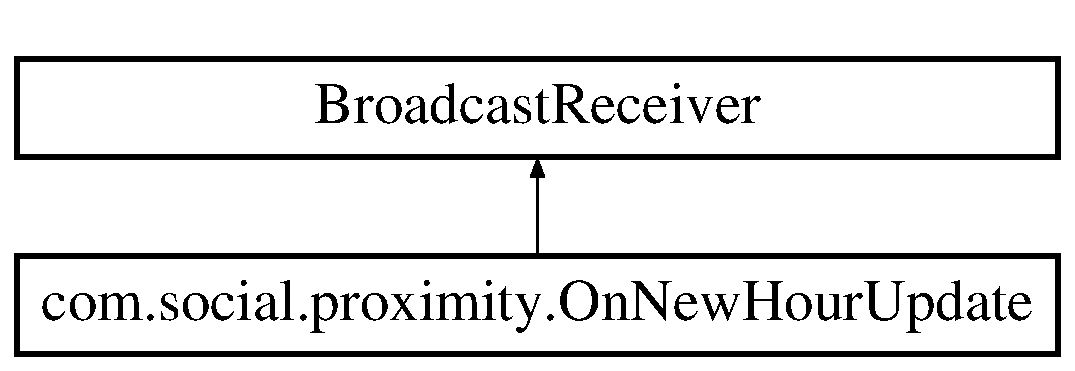
\includegraphics[height=2.000000cm]{classcom_1_1social_1_1proximity_1_1_on_new_hour_update}
\end{center}
\end{figure}
\subsection*{Public Member Functions}
\begin{DoxyCompactItemize}
\item 
\hyperlink{classcom_1_1social_1_1proximity_1_1_on_new_hour_update_abd74ec78f0b1aa902641a2bbf868bbe7}{On\+New\+Hour\+Update} (\hyperlink{classcom_1_1social_1_1proximity_1_1_database_functions}{Database\+Functions} datasource2)
\item 
void \hyperlink{classcom_1_1social_1_1proximity_1_1_on_new_hour_update_a38534c234c903ea13d2321d11c85d72d}{on\+Receive} (Context context, Intent intent)
\item 
int \hyperlink{classcom_1_1social_1_1proximity_1_1_on_new_hour_update_af48a45ab9f45c3a5892c317c5e075231}{get\+Time\+Slot} ()
\item 
void \hyperlink{classcom_1_1social_1_1proximity_1_1_on_new_hour_update_a2f97517684a2248a9d1928c1927cdae6}{show\+Devices\+On\+D\+B} ()
\end{DoxyCompactItemize}
\subsection*{Static Public Attributes}
\begin{DoxyCompactItemize}
\item 
static final String \hyperlink{classcom_1_1social_1_1proximity_1_1_on_new_hour_update_a4d16e6c5468afd333dc75b972efc05e9}{N\+E\+W\+\_\+\+H\+O\+U\+R} = \char`\"{}android.\+intent.\+action.\+N\+E\+W\+H\+O\+U\+R\char`\"{}
\end{DoxyCompactItemize}
\subsection*{Private Member Functions}
\begin{DoxyCompactItemize}
\item 
void \hyperlink{classcom_1_1social_1_1proximity_1_1_on_new_hour_update_a818ac6abd2ca17ec02dc3cc8f553c1f5}{notify\+Data\+Base\+Change} ()
\item 
void \hyperlink{classcom_1_1social_1_1proximity_1_1_on_new_hour_update_a7234323761f300d5b47728b0dc48d47f}{write\+To\+S\+D} (String text)
\end{DoxyCompactItemize}
\subsection*{Private Attributes}
\begin{DoxyCompactItemize}
\item 
\hyperlink{classcom_1_1social_1_1proximity_1_1_database_functions}{Database\+Functions} \hyperlink{classcom_1_1social_1_1proximity_1_1_on_new_hour_update_adf8f88328e9cf6ed2635fbd77ce1854f}{datasource}
\item 
int \hyperlink{classcom_1_1social_1_1proximity_1_1_on_new_hour_update_ab30d5827d79a03141a1c108da2b08e01}{day} = 1
\item 
Array\+List$<$ \hyperlink{interfacecom_1_1social_1_1proximity_1_1_data_base_change_listener}{Data\+Base\+Change\+Listener} $>$ \hyperlink{classcom_1_1social_1_1proximity_1_1_on_new_hour_update_afd3e5f40366b5d77fe49e17a00fb3cb1}{listeners} = new Array\+List$<$\hyperlink{interfacecom_1_1social_1_1proximity_1_1_data_base_change_listener}{Data\+Base\+Change\+Listener}$>$ ()
\end{DoxyCompactItemize}


\subsection{Constructor \& Destructor Documentation}
\hypertarget{classcom_1_1social_1_1proximity_1_1_on_new_hour_update_abd74ec78f0b1aa902641a2bbf868bbe7}{}\index{com\+::social\+::proximity\+::\+On\+New\+Hour\+Update@{com\+::social\+::proximity\+::\+On\+New\+Hour\+Update}!On\+New\+Hour\+Update@{On\+New\+Hour\+Update}}
\index{On\+New\+Hour\+Update@{On\+New\+Hour\+Update}!com\+::social\+::proximity\+::\+On\+New\+Hour\+Update@{com\+::social\+::proximity\+::\+On\+New\+Hour\+Update}}
\subsubsection[{On\+New\+Hour\+Update(\+Database\+Functions datasource2)}]{\setlength{\rightskip}{0pt plus 5cm}com.\+social.\+proximity.\+On\+New\+Hour\+Update.\+On\+New\+Hour\+Update (
\begin{DoxyParamCaption}
\item[{{\bf Database\+Functions}}]{datasource2}
\end{DoxyParamCaption}
)}\label{classcom_1_1social_1_1proximity_1_1_on_new_hour_update_abd74ec78f0b1aa902641a2bbf868bbe7}
\hyperlink{classcom_1_1social_1_1proximity_1_1_on_new_hour_update}{On\+New\+Hour\+Update} constructor. 
\begin{DoxyParams}{Parameters}
{\em datasource2} & The \hyperlink{classcom_1_1social_1_1proximity_1_1_database_functions}{Database\+Functions} object that allows the creation and handling of tables for social proximity computation. \\
\hline
\end{DoxyParams}


\subsection{Member Function Documentation}
\hypertarget{classcom_1_1social_1_1proximity_1_1_on_new_hour_update_af48a45ab9f45c3a5892c317c5e075231}{}\index{com\+::social\+::proximity\+::\+On\+New\+Hour\+Update@{com\+::social\+::proximity\+::\+On\+New\+Hour\+Update}!get\+Time\+Slot@{get\+Time\+Slot}}
\index{get\+Time\+Slot@{get\+Time\+Slot}!com\+::social\+::proximity\+::\+On\+New\+Hour\+Update@{com\+::social\+::proximity\+::\+On\+New\+Hour\+Update}}
\subsubsection[{get\+Time\+Slot()}]{\setlength{\rightskip}{0pt plus 5cm}int com.\+social.\+proximity.\+On\+New\+Hour\+Update.\+get\+Time\+Slot (
\begin{DoxyParamCaption}
{}
\end{DoxyParamCaption}
)}\label{classcom_1_1social_1_1proximity_1_1_on_new_hour_update_af48a45ab9f45c3a5892c317c5e075231}
Provides the current time slot. \begin{DoxyReturn}{Returns}
current\+Time\+Slot The actual time slot. 
\end{DoxyReturn}
\hypertarget{classcom_1_1social_1_1proximity_1_1_on_new_hour_update_a818ac6abd2ca17ec02dc3cc8f553c1f5}{}\index{com\+::social\+::proximity\+::\+On\+New\+Hour\+Update@{com\+::social\+::proximity\+::\+On\+New\+Hour\+Update}!notify\+Data\+Base\+Change@{notify\+Data\+Base\+Change}}
\index{notify\+Data\+Base\+Change@{notify\+Data\+Base\+Change}!com\+::social\+::proximity\+::\+On\+New\+Hour\+Update@{com\+::social\+::proximity\+::\+On\+New\+Hour\+Update}}
\subsubsection[{notify\+Data\+Base\+Change()}]{\setlength{\rightskip}{0pt plus 5cm}void com.\+social.\+proximity.\+On\+New\+Hour\+Update.\+notify\+Data\+Base\+Change (
\begin{DoxyParamCaption}
{}
\end{DoxyParamCaption}
)\hspace{0.3cm}{\ttfamily [private]}}\label{classcom_1_1social_1_1proximity_1_1_on_new_hour_update_a818ac6abd2ca17ec02dc3cc8f553c1f5}
Notifies a database change to the listeners. \hypertarget{classcom_1_1social_1_1proximity_1_1_on_new_hour_update_a38534c234c903ea13d2321d11c85d72d}{}\index{com\+::social\+::proximity\+::\+On\+New\+Hour\+Update@{com\+::social\+::proximity\+::\+On\+New\+Hour\+Update}!on\+Receive@{on\+Receive}}
\index{on\+Receive@{on\+Receive}!com\+::social\+::proximity\+::\+On\+New\+Hour\+Update@{com\+::social\+::proximity\+::\+On\+New\+Hour\+Update}}
\subsubsection[{on\+Receive(\+Context context, Intent intent)}]{\setlength{\rightskip}{0pt plus 5cm}void com.\+social.\+proximity.\+On\+New\+Hour\+Update.\+on\+Receive (
\begin{DoxyParamCaption}
\item[{Context}]{context, }
\item[{Intent}]{intent}
\end{DoxyParamCaption}
)}\label{classcom_1_1social_1_1proximity_1_1_on_new_hour_update_a38534c234c903ea13d2321d11c85d72d}
\hypertarget{classcom_1_1social_1_1proximity_1_1_on_new_hour_update_a2f97517684a2248a9d1928c1927cdae6}{}\index{com\+::social\+::proximity\+::\+On\+New\+Hour\+Update@{com\+::social\+::proximity\+::\+On\+New\+Hour\+Update}!show\+Devices\+On\+D\+B@{show\+Devices\+On\+D\+B}}
\index{show\+Devices\+On\+D\+B@{show\+Devices\+On\+D\+B}!com\+::social\+::proximity\+::\+On\+New\+Hour\+Update@{com\+::social\+::proximity\+::\+On\+New\+Hour\+Update}}
\subsubsection[{show\+Devices\+On\+D\+B()}]{\setlength{\rightskip}{0pt plus 5cm}void com.\+social.\+proximity.\+On\+New\+Hour\+Update.\+show\+Devices\+On\+D\+B (
\begin{DoxyParamCaption}
{}
\end{DoxyParamCaption}
)}\label{classcom_1_1social_1_1proximity_1_1_on_new_hour_update_a2f97517684a2248a9d1928c1927cdae6}
Shows the Bluetooth devices stored on the D\+B. For debugging purposes. \hypertarget{classcom_1_1social_1_1proximity_1_1_on_new_hour_update_a7234323761f300d5b47728b0dc48d47f}{}\index{com\+::social\+::proximity\+::\+On\+New\+Hour\+Update@{com\+::social\+::proximity\+::\+On\+New\+Hour\+Update}!write\+To\+S\+D@{write\+To\+S\+D}}
\index{write\+To\+S\+D@{write\+To\+S\+D}!com\+::social\+::proximity\+::\+On\+New\+Hour\+Update@{com\+::social\+::proximity\+::\+On\+New\+Hour\+Update}}
\subsubsection[{write\+To\+S\+D(\+String text)}]{\setlength{\rightskip}{0pt plus 5cm}void com.\+social.\+proximity.\+On\+New\+Hour\+Update.\+write\+To\+S\+D (
\begin{DoxyParamCaption}
\item[{String}]{text}
\end{DoxyParamCaption}
)\hspace{0.3cm}{\ttfamily [private]}}\label{classcom_1_1social_1_1proximity_1_1_on_new_hour_update_a7234323761f300d5b47728b0dc48d47f}
Writes on a file for Bluetooth debugging. 

\subsection{Member Data Documentation}
\hypertarget{classcom_1_1social_1_1proximity_1_1_on_new_hour_update_adf8f88328e9cf6ed2635fbd77ce1854f}{}\index{com\+::social\+::proximity\+::\+On\+New\+Hour\+Update@{com\+::social\+::proximity\+::\+On\+New\+Hour\+Update}!datasource@{datasource}}
\index{datasource@{datasource}!com\+::social\+::proximity\+::\+On\+New\+Hour\+Update@{com\+::social\+::proximity\+::\+On\+New\+Hour\+Update}}
\subsubsection[{datasource}]{\setlength{\rightskip}{0pt plus 5cm}{\bf Database\+Functions} com.\+social.\+proximity.\+On\+New\+Hour\+Update.\+datasource\hspace{0.3cm}{\ttfamily [private]}}\label{classcom_1_1social_1_1proximity_1_1_on_new_hour_update_adf8f88328e9cf6ed2635fbd77ce1854f}
\hypertarget{classcom_1_1social_1_1proximity_1_1_on_new_hour_update_ab30d5827d79a03141a1c108da2b08e01}{}\index{com\+::social\+::proximity\+::\+On\+New\+Hour\+Update@{com\+::social\+::proximity\+::\+On\+New\+Hour\+Update}!day@{day}}
\index{day@{day}!com\+::social\+::proximity\+::\+On\+New\+Hour\+Update@{com\+::social\+::proximity\+::\+On\+New\+Hour\+Update}}
\subsubsection[{day}]{\setlength{\rightskip}{0pt plus 5cm}int com.\+social.\+proximity.\+On\+New\+Hour\+Update.\+day = 1\hspace{0.3cm}{\ttfamily [private]}}\label{classcom_1_1social_1_1proximity_1_1_on_new_hour_update_ab30d5827d79a03141a1c108da2b08e01}
\hypertarget{classcom_1_1social_1_1proximity_1_1_on_new_hour_update_afd3e5f40366b5d77fe49e17a00fb3cb1}{}\index{com\+::social\+::proximity\+::\+On\+New\+Hour\+Update@{com\+::social\+::proximity\+::\+On\+New\+Hour\+Update}!listeners@{listeners}}
\index{listeners@{listeners}!com\+::social\+::proximity\+::\+On\+New\+Hour\+Update@{com\+::social\+::proximity\+::\+On\+New\+Hour\+Update}}
\subsubsection[{listeners}]{\setlength{\rightskip}{0pt plus 5cm}Array\+List$<${\bf Data\+Base\+Change\+Listener}$>$ com.\+social.\+proximity.\+On\+New\+Hour\+Update.\+listeners = new Array\+List$<${\bf Data\+Base\+Change\+Listener}$>$ ()\hspace{0.3cm}{\ttfamily [private]}}\label{classcom_1_1social_1_1proximity_1_1_on_new_hour_update_afd3e5f40366b5d77fe49e17a00fb3cb1}
\hypertarget{classcom_1_1social_1_1proximity_1_1_on_new_hour_update_a4d16e6c5468afd333dc75b972efc05e9}{}\index{com\+::social\+::proximity\+::\+On\+New\+Hour\+Update@{com\+::social\+::proximity\+::\+On\+New\+Hour\+Update}!N\+E\+W\+\_\+\+H\+O\+U\+R@{N\+E\+W\+\_\+\+H\+O\+U\+R}}
\index{N\+E\+W\+\_\+\+H\+O\+U\+R@{N\+E\+W\+\_\+\+H\+O\+U\+R}!com\+::social\+::proximity\+::\+On\+New\+Hour\+Update@{com\+::social\+::proximity\+::\+On\+New\+Hour\+Update}}
\subsubsection[{N\+E\+W\+\_\+\+H\+O\+U\+R}]{\setlength{\rightskip}{0pt plus 5cm}final String com.\+social.\+proximity.\+On\+New\+Hour\+Update.\+N\+E\+W\+\_\+\+H\+O\+U\+R = \char`\"{}android.\+intent.\+action.\+N\+E\+W\+H\+O\+U\+R\char`\"{}\hspace{0.3cm}{\ttfamily [static]}}\label{classcom_1_1social_1_1proximity_1_1_on_new_hour_update_a4d16e6c5468afd333dc75b972efc05e9}


The documentation for this class was generated from the following file\+:\begin{DoxyCompactItemize}
\item 
src/com/social/proximity/\hyperlink{_on_new_hour_update_8java}{On\+New\+Hour\+Update.\+java}\end{DoxyCompactItemize}

\hypertarget{classcom_1_1social_1_1proximity_1_1_social_proximity}{}\section{com.\+social.\+proximity.\+Social\+Proximity Class Reference}
\label{classcom_1_1social_1_1proximity_1_1_social_proximity}\index{com.\+social.\+proximity.\+Social\+Proximity@{com.\+social.\+proximity.\+Social\+Proximity}}
\subsection*{Classes}
\begin{DoxyCompactItemize}
\item 
class \hyperlink{classcom_1_1social_1_1proximity_1_1_social_proximity_1_1_custom_comparator}{Custom\+Comparator}
\item 
class {\bfseries Service\+B\+T\+Listener}
\end{DoxyCompactItemize}
\subsection*{Public Member Functions}
\begin{DoxyCompactItemize}
\item 
\hyperlink{classcom_1_1social_1_1proximity_1_1_social_proximity_aca9e6f96e31a9714fed5967a7710ad1e}{Social\+Proximity} (Context \hyperlink{classcom_1_1social_1_1proximity_1_1_social_proximity_a094349a2f8b31f6f13353abec962f0a4}{context}, \hyperlink{classcom_1_1social_1_1proximity_1_1_database_functions}{Database\+Functions} \hyperlink{classcom_1_1social_1_1proximity_1_1_social_proximity_ac36be388d1519a9c1ec298bcac0aa3f2}{datasource})
\item 
boolean \hyperlink{classcom_1_1social_1_1proximity_1_1_social_proximity_a5cd69f250d4aca9e436760ce078e762b}{is\+Device\+On\+D\+B} (String device\+Add)
\item 
Array\+List$<$ \hyperlink{classcom_1_1social_1_1proximity_1_1_social_weight}{Social\+Weight} $>$ \hyperlink{classcom_1_1social_1_1proximity_1_1_social_proximity_ae1acae13d8ea15aedcd8d7c758f45aef}{get\+Social\+Weight\+Details} ()
\item 
void \hyperlink{classcom_1_1social_1_1proximity_1_1_social_proximity_aeea1aa00b7a490fdf71eeb9cb68ab9dd}{close} (Context \hyperlink{classcom_1_1social_1_1proximity_1_1_social_proximity_a094349a2f8b31f6f13353abec962f0a4}{context})
\item 
int \hyperlink{classcom_1_1social_1_1proximity_1_1_social_proximity_a2f777f371e2f1b98c1f6d3d476ecd614}{get\+Time\+Slot} ()
\end{DoxyCompactItemize}
\subsection*{Static Public Attributes}
\begin{DoxyCompactItemize}
\item 
static final String \hyperlink{classcom_1_1social_1_1proximity_1_1_social_proximity_a4019a76ca6d383cb77b9e81f1b7c2cca}{D\+A\+T\+A\+B\+A\+S\+E\+\_\+\+C\+H\+A\+N\+G\+E} = \char`\"{}com.\+social.\+proximity.\+C\+H\+A\+N\+G\+E\char`\"{}
\end{DoxyCompactItemize}
\subsection*{Private Member Functions}
\begin{DoxyCompactItemize}
\item 
void \hyperlink{classcom_1_1social_1_1proximity_1_1_social_proximity_a64e73fce0d2fe51898d7b6218e2fd744}{notify\+Data\+Base\+Change} ()
\item 
void \hyperlink{classcom_1_1social_1_1proximity_1_1_social_proximity_aa5ed8999ce753a87c15272798eaf99be}{write\+To\+S\+D} (String text)
\end{DoxyCompactItemize}
\subsection*{Private Attributes}
\begin{DoxyCompactItemize}
\item 
final String \hyperlink{classcom_1_1social_1_1proximity_1_1_social_proximity_ac2be9322648a27ced5d00e8eae40bac4}{T\+A\+G} = \char`\"{}Bluetooth Testing\char`\"{}
\item 
\hyperlink{classcom_1_1social_1_1proximity_1_1_b_t_manager}{B\+T\+Manager} \hyperlink{classcom_1_1social_1_1proximity_1_1_social_proximity_a7833a112a845f6ff11f5101bbd40d98b}{my\+B\+T\+Manager}
\item 
Service\+B\+T\+Listener \hyperlink{classcom_1_1social_1_1proximity_1_1_social_proximity_a54409038923d01acde8779da84812350}{bt\+Listener}
\item 
Alarm\+Manager \hyperlink{classcom_1_1social_1_1proximity_1_1_social_proximity_afddec12a7de1b3e5e9dc86da413da78f}{alarm\+Mgr}
\item 
Pending\+Intent \hyperlink{classcom_1_1social_1_1proximity_1_1_social_proximity_ae91f5ac95c6c68993a47e70e8e7f5854}{alarm\+Intent}
\item 
\hyperlink{classcom_1_1social_1_1proximity_1_1_on_new_hour_update}{On\+New\+Hour\+Update} \hyperlink{classcom_1_1social_1_1proximity_1_1_social_proximity_ab3d29f906dd80ba99f79bbe848658294}{new\+Hour}
\item 
Context \hyperlink{classcom_1_1social_1_1proximity_1_1_social_proximity_a094349a2f8b31f6f13353abec962f0a4}{context}
\item 
\hyperlink{classcom_1_1social_1_1proximity_1_1_database_functions}{Database\+Functions} \hyperlink{classcom_1_1social_1_1proximity_1_1_social_proximity_ac36be388d1519a9c1ec298bcac0aa3f2}{datasource}
\end{DoxyCompactItemize}


\subsection{Constructor \& Destructor Documentation}
\hypertarget{classcom_1_1social_1_1proximity_1_1_social_proximity_aca9e6f96e31a9714fed5967a7710ad1e}{}\index{com\+::social\+::proximity\+::\+Social\+Proximity@{com\+::social\+::proximity\+::\+Social\+Proximity}!Social\+Proximity@{Social\+Proximity}}
\index{Social\+Proximity@{Social\+Proximity}!com\+::social\+::proximity\+::\+Social\+Proximity@{com\+::social\+::proximity\+::\+Social\+Proximity}}
\subsubsection[{Social\+Proximity(\+Context context, Database\+Functions datasource)}]{\setlength{\rightskip}{0pt plus 5cm}com.\+social.\+proximity.\+Social\+Proximity.\+Social\+Proximity (
\begin{DoxyParamCaption}
\item[{Context}]{context, }
\item[{{\bf Database\+Functions}}]{datasource}
\end{DoxyParamCaption}
)}\label{classcom_1_1social_1_1proximity_1_1_social_proximity_aca9e6f96e31a9714fed5967a7710ad1e}
\hyperlink{classcom_1_1social_1_1proximity_1_1_social_proximity}{Social\+Proximity} constructor. 
\begin{DoxyParams}{Parameters}
{\em context} & The context which provides access to resources and specific classes of the application. \\
\hline
{\em datasource} & The object that allows the handling of tables for social proximity computation. \\
\hline
\end{DoxyParams}


\subsection{Member Function Documentation}
\hypertarget{classcom_1_1social_1_1proximity_1_1_social_proximity_aeea1aa00b7a490fdf71eeb9cb68ab9dd}{}\index{com\+::social\+::proximity\+::\+Social\+Proximity@{com\+::social\+::proximity\+::\+Social\+Proximity}!close@{close}}
\index{close@{close}!com\+::social\+::proximity\+::\+Social\+Proximity@{com\+::social\+::proximity\+::\+Social\+Proximity}}
\subsubsection[{close(\+Context context)}]{\setlength{\rightskip}{0pt plus 5cm}void com.\+social.\+proximity.\+Social\+Proximity.\+close (
\begin{DoxyParamCaption}
\item[{Context}]{context}
\end{DoxyParamCaption}
)}\label{classcom_1_1social_1_1proximity_1_1_social_proximity_aeea1aa00b7a490fdf71eeb9cb68ab9dd}
Stops Bluetooth-\/related tasks (i.\+e., scanning, unregister broadcast receivers) 
\begin{DoxyParams}{Parameters}
{\em context} & The context which provides access to resources and specific classes of the application \\
\hline
\end{DoxyParams}
\hypertarget{classcom_1_1social_1_1proximity_1_1_social_proximity_ae1acae13d8ea15aedcd8d7c758f45aef}{}\index{com\+::social\+::proximity\+::\+Social\+Proximity@{com\+::social\+::proximity\+::\+Social\+Proximity}!get\+Social\+Weight\+Details@{get\+Social\+Weight\+Details}}
\index{get\+Social\+Weight\+Details@{get\+Social\+Weight\+Details}!com\+::social\+::proximity\+::\+Social\+Proximity@{com\+::social\+::proximity\+::\+Social\+Proximity}}
\subsubsection[{get\+Social\+Weight\+Details()}]{\setlength{\rightskip}{0pt plus 5cm}Array\+List$<${\bf Social\+Weight}$>$ com.\+social.\+proximity.\+Social\+Proximity.\+get\+Social\+Weight\+Details (
\begin{DoxyParamCaption}
{}
\end{DoxyParamCaption}
)}\label{classcom_1_1social_1_1proximity_1_1_social_proximity_ae1acae13d8ea15aedcd8d7c758f45aef}
Provides a list of encountered peers and the social weights towards them. \begin{DoxyReturn}{Returns}
list\+Weights List of peers with weights sorted in a descending way. 
\end{DoxyReturn}
\hypertarget{classcom_1_1social_1_1proximity_1_1_social_proximity_a2f777f371e2f1b98c1f6d3d476ecd614}{}\index{com\+::social\+::proximity\+::\+Social\+Proximity@{com\+::social\+::proximity\+::\+Social\+Proximity}!get\+Time\+Slot@{get\+Time\+Slot}}
\index{get\+Time\+Slot@{get\+Time\+Slot}!com\+::social\+::proximity\+::\+Social\+Proximity@{com\+::social\+::proximity\+::\+Social\+Proximity}}
\subsubsection[{get\+Time\+Slot()}]{\setlength{\rightskip}{0pt plus 5cm}int com.\+social.\+proximity.\+Social\+Proximity.\+get\+Time\+Slot (
\begin{DoxyParamCaption}
{}
\end{DoxyParamCaption}
)}\label{classcom_1_1social_1_1proximity_1_1_social_proximity_a2f777f371e2f1b98c1f6d3d476ecd614}
Provides the current time slot \begin{DoxyReturn}{Returns}
current\+Time\+Slot The actual time slot 
\end{DoxyReturn}
\hypertarget{classcom_1_1social_1_1proximity_1_1_social_proximity_a5cd69f250d4aca9e436760ce078e762b}{}\index{com\+::social\+::proximity\+::\+Social\+Proximity@{com\+::social\+::proximity\+::\+Social\+Proximity}!is\+Device\+On\+D\+B@{is\+Device\+On\+D\+B}}
\index{is\+Device\+On\+D\+B@{is\+Device\+On\+D\+B}!com\+::social\+::proximity\+::\+Social\+Proximity@{com\+::social\+::proximity\+::\+Social\+Proximity}}
\subsubsection[{is\+Device\+On\+D\+B(\+String device\+Add)}]{\setlength{\rightskip}{0pt plus 5cm}boolean com.\+social.\+proximity.\+Social\+Proximity.\+is\+Device\+On\+D\+B (
\begin{DoxyParamCaption}
\item[{String}]{device\+Add}
\end{DoxyParamCaption}
)}\label{classcom_1_1social_1_1proximity_1_1_social_proximity_a5cd69f250d4aca9e436760ce078e762b}
Checks whether the device is in D\+B. 
\begin{DoxyParams}{Parameters}
{\em device\+Add} & The device M\+A\+C address. \\
\hline
\end{DoxyParams}
\begin{DoxyReturn}{Returns}
true if device is in D\+B, false otherwise 
\end{DoxyReturn}
\hypertarget{classcom_1_1social_1_1proximity_1_1_social_proximity_a64e73fce0d2fe51898d7b6218e2fd744}{}\index{com\+::social\+::proximity\+::\+Social\+Proximity@{com\+::social\+::proximity\+::\+Social\+Proximity}!notify\+Data\+Base\+Change@{notify\+Data\+Base\+Change}}
\index{notify\+Data\+Base\+Change@{notify\+Data\+Base\+Change}!com\+::social\+::proximity\+::\+Social\+Proximity@{com\+::social\+::proximity\+::\+Social\+Proximity}}
\subsubsection[{notify\+Data\+Base\+Change()}]{\setlength{\rightskip}{0pt plus 5cm}void com.\+social.\+proximity.\+Social\+Proximity.\+notify\+Data\+Base\+Change (
\begin{DoxyParamCaption}
{}
\end{DoxyParamCaption}
)\hspace{0.3cm}{\ttfamily [private]}}\label{classcom_1_1social_1_1proximity_1_1_social_proximity_a64e73fce0d2fe51898d7b6218e2fd744}
Notifies a database change to the listeners. \hypertarget{classcom_1_1social_1_1proximity_1_1_social_proximity_aa5ed8999ce753a87c15272798eaf99be}{}\index{com\+::social\+::proximity\+::\+Social\+Proximity@{com\+::social\+::proximity\+::\+Social\+Proximity}!write\+To\+S\+D@{write\+To\+S\+D}}
\index{write\+To\+S\+D@{write\+To\+S\+D}!com\+::social\+::proximity\+::\+Social\+Proximity@{com\+::social\+::proximity\+::\+Social\+Proximity}}
\subsubsection[{write\+To\+S\+D(\+String text)}]{\setlength{\rightskip}{0pt plus 5cm}void com.\+social.\+proximity.\+Social\+Proximity.\+write\+To\+S\+D (
\begin{DoxyParamCaption}
\item[{String}]{text}
\end{DoxyParamCaption}
)\hspace{0.3cm}{\ttfamily [private]}}\label{classcom_1_1social_1_1proximity_1_1_social_proximity_aa5ed8999ce753a87c15272798eaf99be}
Writes on a file for Bluetooth debugging 

\subsection{Member Data Documentation}
\hypertarget{classcom_1_1social_1_1proximity_1_1_social_proximity_ae91f5ac95c6c68993a47e70e8e7f5854}{}\index{com\+::social\+::proximity\+::\+Social\+Proximity@{com\+::social\+::proximity\+::\+Social\+Proximity}!alarm\+Intent@{alarm\+Intent}}
\index{alarm\+Intent@{alarm\+Intent}!com\+::social\+::proximity\+::\+Social\+Proximity@{com\+::social\+::proximity\+::\+Social\+Proximity}}
\subsubsection[{alarm\+Intent}]{\setlength{\rightskip}{0pt plus 5cm}Pending\+Intent com.\+social.\+proximity.\+Social\+Proximity.\+alarm\+Intent\hspace{0.3cm}{\ttfamily [private]}}\label{classcom_1_1social_1_1proximity_1_1_social_proximity_ae91f5ac95c6c68993a47e70e8e7f5854}
\hypertarget{classcom_1_1social_1_1proximity_1_1_social_proximity_afddec12a7de1b3e5e9dc86da413da78f}{}\index{com\+::social\+::proximity\+::\+Social\+Proximity@{com\+::social\+::proximity\+::\+Social\+Proximity}!alarm\+Mgr@{alarm\+Mgr}}
\index{alarm\+Mgr@{alarm\+Mgr}!com\+::social\+::proximity\+::\+Social\+Proximity@{com\+::social\+::proximity\+::\+Social\+Proximity}}
\subsubsection[{alarm\+Mgr}]{\setlength{\rightskip}{0pt plus 5cm}Alarm\+Manager com.\+social.\+proximity.\+Social\+Proximity.\+alarm\+Mgr\hspace{0.3cm}{\ttfamily [private]}}\label{classcom_1_1social_1_1proximity_1_1_social_proximity_afddec12a7de1b3e5e9dc86da413da78f}
\hypertarget{classcom_1_1social_1_1proximity_1_1_social_proximity_a54409038923d01acde8779da84812350}{}\index{com\+::social\+::proximity\+::\+Social\+Proximity@{com\+::social\+::proximity\+::\+Social\+Proximity}!bt\+Listener@{bt\+Listener}}
\index{bt\+Listener@{bt\+Listener}!com\+::social\+::proximity\+::\+Social\+Proximity@{com\+::social\+::proximity\+::\+Social\+Proximity}}
\subsubsection[{bt\+Listener}]{\setlength{\rightskip}{0pt plus 5cm}Service\+B\+T\+Listener com.\+social.\+proximity.\+Social\+Proximity.\+bt\+Listener\hspace{0.3cm}{\ttfamily [private]}}\label{classcom_1_1social_1_1proximity_1_1_social_proximity_a54409038923d01acde8779da84812350}
\hypertarget{classcom_1_1social_1_1proximity_1_1_social_proximity_a094349a2f8b31f6f13353abec962f0a4}{}\index{com\+::social\+::proximity\+::\+Social\+Proximity@{com\+::social\+::proximity\+::\+Social\+Proximity}!context@{context}}
\index{context@{context}!com\+::social\+::proximity\+::\+Social\+Proximity@{com\+::social\+::proximity\+::\+Social\+Proximity}}
\subsubsection[{context}]{\setlength{\rightskip}{0pt plus 5cm}Context com.\+social.\+proximity.\+Social\+Proximity.\+context\hspace{0.3cm}{\ttfamily [private]}}\label{classcom_1_1social_1_1proximity_1_1_social_proximity_a094349a2f8b31f6f13353abec962f0a4}
\hypertarget{classcom_1_1social_1_1proximity_1_1_social_proximity_a4019a76ca6d383cb77b9e81f1b7c2cca}{}\index{com\+::social\+::proximity\+::\+Social\+Proximity@{com\+::social\+::proximity\+::\+Social\+Proximity}!D\+A\+T\+A\+B\+A\+S\+E\+\_\+\+C\+H\+A\+N\+G\+E@{D\+A\+T\+A\+B\+A\+S\+E\+\_\+\+C\+H\+A\+N\+G\+E}}
\index{D\+A\+T\+A\+B\+A\+S\+E\+\_\+\+C\+H\+A\+N\+G\+E@{D\+A\+T\+A\+B\+A\+S\+E\+\_\+\+C\+H\+A\+N\+G\+E}!com\+::social\+::proximity\+::\+Social\+Proximity@{com\+::social\+::proximity\+::\+Social\+Proximity}}
\subsubsection[{D\+A\+T\+A\+B\+A\+S\+E\+\_\+\+C\+H\+A\+N\+G\+E}]{\setlength{\rightskip}{0pt plus 5cm}final String com.\+social.\+proximity.\+Social\+Proximity.\+D\+A\+T\+A\+B\+A\+S\+E\+\_\+\+C\+H\+A\+N\+G\+E = \char`\"{}com.\+social.\+proximity.\+C\+H\+A\+N\+G\+E\char`\"{}\hspace{0.3cm}{\ttfamily [static]}}\label{classcom_1_1social_1_1proximity_1_1_social_proximity_a4019a76ca6d383cb77b9e81f1b7c2cca}
\hypertarget{classcom_1_1social_1_1proximity_1_1_social_proximity_ac36be388d1519a9c1ec298bcac0aa3f2}{}\index{com\+::social\+::proximity\+::\+Social\+Proximity@{com\+::social\+::proximity\+::\+Social\+Proximity}!datasource@{datasource}}
\index{datasource@{datasource}!com\+::social\+::proximity\+::\+Social\+Proximity@{com\+::social\+::proximity\+::\+Social\+Proximity}}
\subsubsection[{datasource}]{\setlength{\rightskip}{0pt plus 5cm}{\bf Database\+Functions} com.\+social.\+proximity.\+Social\+Proximity.\+datasource\hspace{0.3cm}{\ttfamily [private]}}\label{classcom_1_1social_1_1proximity_1_1_social_proximity_ac36be388d1519a9c1ec298bcac0aa3f2}
\hypertarget{classcom_1_1social_1_1proximity_1_1_social_proximity_a7833a112a845f6ff11f5101bbd40d98b}{}\index{com\+::social\+::proximity\+::\+Social\+Proximity@{com\+::social\+::proximity\+::\+Social\+Proximity}!my\+B\+T\+Manager@{my\+B\+T\+Manager}}
\index{my\+B\+T\+Manager@{my\+B\+T\+Manager}!com\+::social\+::proximity\+::\+Social\+Proximity@{com\+::social\+::proximity\+::\+Social\+Proximity}}
\subsubsection[{my\+B\+T\+Manager}]{\setlength{\rightskip}{0pt plus 5cm}{\bf B\+T\+Manager} com.\+social.\+proximity.\+Social\+Proximity.\+my\+B\+T\+Manager\hspace{0.3cm}{\ttfamily [private]}}\label{classcom_1_1social_1_1proximity_1_1_social_proximity_a7833a112a845f6ff11f5101bbd40d98b}
\hypertarget{classcom_1_1social_1_1proximity_1_1_social_proximity_ab3d29f906dd80ba99f79bbe848658294}{}\index{com\+::social\+::proximity\+::\+Social\+Proximity@{com\+::social\+::proximity\+::\+Social\+Proximity}!new\+Hour@{new\+Hour}}
\index{new\+Hour@{new\+Hour}!com\+::social\+::proximity\+::\+Social\+Proximity@{com\+::social\+::proximity\+::\+Social\+Proximity}}
\subsubsection[{new\+Hour}]{\setlength{\rightskip}{0pt plus 5cm}{\bf On\+New\+Hour\+Update} com.\+social.\+proximity.\+Social\+Proximity.\+new\+Hour\hspace{0.3cm}{\ttfamily [private]}}\label{classcom_1_1social_1_1proximity_1_1_social_proximity_ab3d29f906dd80ba99f79bbe848658294}
\hypertarget{classcom_1_1social_1_1proximity_1_1_social_proximity_ac2be9322648a27ced5d00e8eae40bac4}{}\index{com\+::social\+::proximity\+::\+Social\+Proximity@{com\+::social\+::proximity\+::\+Social\+Proximity}!T\+A\+G@{T\+A\+G}}
\index{T\+A\+G@{T\+A\+G}!com\+::social\+::proximity\+::\+Social\+Proximity@{com\+::social\+::proximity\+::\+Social\+Proximity}}
\subsubsection[{T\+A\+G}]{\setlength{\rightskip}{0pt plus 5cm}final String com.\+social.\+proximity.\+Social\+Proximity.\+T\+A\+G = \char`\"{}Bluetooth Testing\char`\"{}\hspace{0.3cm}{\ttfamily [private]}}\label{classcom_1_1social_1_1proximity_1_1_social_proximity_ac2be9322648a27ced5d00e8eae40bac4}


The documentation for this class was generated from the following file\+:\begin{DoxyCompactItemize}
\item 
src/com/social/proximity/\hyperlink{_social_proximity_8java}{Social\+Proximity.\+java}\end{DoxyCompactItemize}

\hypertarget{classcom_1_1social_1_1proximity_1_1_social_weight}{}\section{com.\+social.\+proximity.\+Social\+Weight Class Reference}
\label{classcom_1_1social_1_1proximity_1_1_social_weight}\index{com.\+social.\+proximity.\+Social\+Weight@{com.\+social.\+proximity.\+Social\+Weight}}
Inheritance diagram for com.\+social.\+proximity.\+Social\+Weight\+:\begin{figure}[H]
\begin{center}
\leavevmode
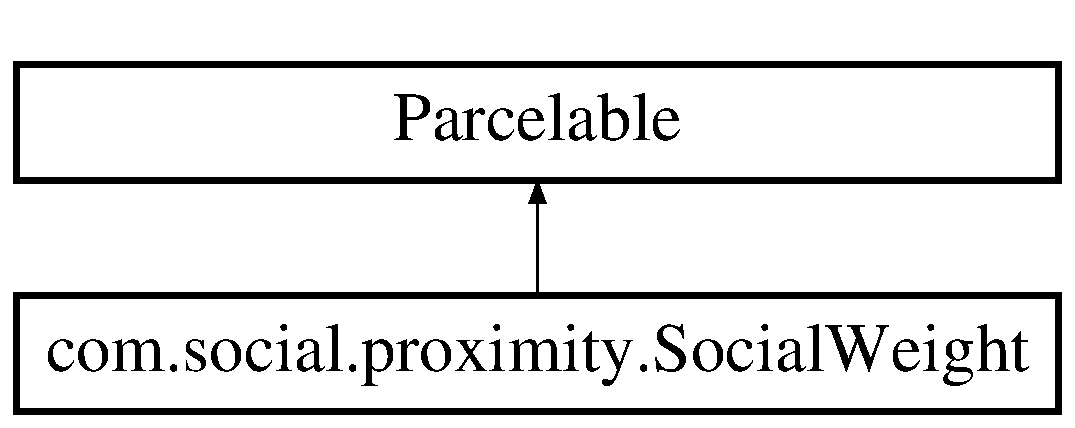
\includegraphics[height=2.000000cm]{classcom_1_1social_1_1proximity_1_1_social_weight}
\end{center}
\end{figure}
\subsection*{Public Member Functions}
\begin{DoxyCompactItemize}
\item 
void \hyperlink{classcom_1_1social_1_1proximity_1_1_social_weight_a660888808784a039fa9e62761f42cb56}{set\+Mac\+Address} (String \hyperlink{classcom_1_1social_1_1proximity_1_1_social_weight_aed1c91d7a26e69969def12d0fe48e4a4}{m\+Mac\+Address})
\item 
String \hyperlink{classcom_1_1social_1_1proximity_1_1_social_weight_afc40805bb79878bcc3b2b1ed1b90aabb}{get\+Mac\+Address} ()
\item 
void \hyperlink{classcom_1_1social_1_1proximity_1_1_social_weight_adb58e2271cb3327f2eb645ffc733ad2e}{set\+Device\+Name} (String \hyperlink{classcom_1_1social_1_1proximity_1_1_social_weight_acd7f605dbf810c5d601273cf70b6f0d9}{m\+Device\+Name})
\item 
String \hyperlink{classcom_1_1social_1_1proximity_1_1_social_weight_abe82b3116319cfc64e8a87be75608f43}{get\+Device\+Name} ()
\item 
void \hyperlink{classcom_1_1social_1_1proximity_1_1_social_weight_a7a5d475fb26ba400ad658109eaaf13ee}{set\+Social\+Weight} (int \hyperlink{classcom_1_1social_1_1proximity_1_1_social_weight_ae500aa203aee4493c114fbd2bbeb654c}{m\+Social\+Weight})
\item 
int \hyperlink{classcom_1_1social_1_1proximity_1_1_social_weight_a902b1316ba8dd9bcca23e6bef85271a4}{get\+Social\+Weight} ()
\item 
\hyperlink{classcom_1_1social_1_1proximity_1_1_social_weight_a16b05f97acc80b23f188bb3b9b4fe62d}{Social\+Weight} ()
\item 
\hyperlink{classcom_1_1social_1_1proximity_1_1_social_weight_ae81d301c0fc7ff4b57862afae71777a3}{Social\+Weight} (Parcel source)
\item 
int \hyperlink{classcom_1_1social_1_1proximity_1_1_social_weight_a2ba69bbc7275a8b2a473a3be11cfaa6b}{describe\+Contents} ()
\item 
void \hyperlink{classcom_1_1social_1_1proximity_1_1_social_weight_ad535ed35c415b459848e1f909f9a9af8}{write\+To\+Parcel} (Parcel dest, int flags)
\end{DoxyCompactItemize}
\subsection*{Public Attributes}
\begin{DoxyCompactItemize}
\item 
final Creator \hyperlink{classcom_1_1social_1_1proximity_1_1_social_weight_a009e0d47a26f8b058f002df215d1c463}{C\+R\+E\+A\+T\+O\+R}
\end{DoxyCompactItemize}
\subsection*{Static Public Attributes}
\begin{DoxyCompactItemize}
\item 
static final String \hyperlink{classcom_1_1social_1_1proximity_1_1_social_weight_a1257231715589b7e1fc3dd5804d6eb9b}{social\+Weight\+\_\+key} = \char`\"{}social\+Receiver\char`\"{}
\end{DoxyCompactItemize}
\subsection*{Private Attributes}
\begin{DoxyCompactItemize}
\item 
String \hyperlink{classcom_1_1social_1_1proximity_1_1_social_weight_aed1c91d7a26e69969def12d0fe48e4a4}{m\+Mac\+Address}
\item 
String \hyperlink{classcom_1_1social_1_1proximity_1_1_social_weight_acd7f605dbf810c5d601273cf70b6f0d9}{m\+Device\+Name}
\item 
int \hyperlink{classcom_1_1social_1_1proximity_1_1_social_weight_ae500aa203aee4493c114fbd2bbeb654c}{m\+Social\+Weight}
\end{DoxyCompactItemize}


\subsection{Constructor \& Destructor Documentation}
\hypertarget{classcom_1_1social_1_1proximity_1_1_social_weight_a16b05f97acc80b23f188bb3b9b4fe62d}{}\index{com\+::social\+::proximity\+::\+Social\+Weight@{com\+::social\+::proximity\+::\+Social\+Weight}!Social\+Weight@{Social\+Weight}}
\index{Social\+Weight@{Social\+Weight}!com\+::social\+::proximity\+::\+Social\+Weight@{com\+::social\+::proximity\+::\+Social\+Weight}}
\subsubsection[{Social\+Weight()}]{\setlength{\rightskip}{0pt plus 5cm}com.\+social.\+proximity.\+Social\+Weight.\+Social\+Weight (
\begin{DoxyParamCaption}
{}
\end{DoxyParamCaption}
)}\label{classcom_1_1social_1_1proximity_1_1_social_weight_a16b05f97acc80b23f188bb3b9b4fe62d}
\hyperlink{classcom_1_1social_1_1proximity_1_1_social_weight}{Social\+Weight} constructor. \hypertarget{classcom_1_1social_1_1proximity_1_1_social_weight_ae81d301c0fc7ff4b57862afae71777a3}{}\index{com\+::social\+::proximity\+::\+Social\+Weight@{com\+::social\+::proximity\+::\+Social\+Weight}!Social\+Weight@{Social\+Weight}}
\index{Social\+Weight@{Social\+Weight}!com\+::social\+::proximity\+::\+Social\+Weight@{com\+::social\+::proximity\+::\+Social\+Weight}}
\subsubsection[{Social\+Weight(\+Parcel source)}]{\setlength{\rightskip}{0pt plus 5cm}com.\+social.\+proximity.\+Social\+Weight.\+Social\+Weight (
\begin{DoxyParamCaption}
\item[{Parcel}]{source}
\end{DoxyParamCaption}
)}\label{classcom_1_1social_1_1proximity_1_1_social_weight_ae81d301c0fc7ff4b57862afae71777a3}
\hyperlink{classcom_1_1social_1_1proximity_1_1_social_weight}{Social\+Weight} constructor. 
\begin{DoxyParams}{Parameters}
{\em source} & The object containing the M\+A\+C address, name and social weight towards a device. \\
\hline
\end{DoxyParams}


\subsection{Member Function Documentation}
\hypertarget{classcom_1_1social_1_1proximity_1_1_social_weight_a2ba69bbc7275a8b2a473a3be11cfaa6b}{}\index{com\+::social\+::proximity\+::\+Social\+Weight@{com\+::social\+::proximity\+::\+Social\+Weight}!describe\+Contents@{describe\+Contents}}
\index{describe\+Contents@{describe\+Contents}!com\+::social\+::proximity\+::\+Social\+Weight@{com\+::social\+::proximity\+::\+Social\+Weight}}
\subsubsection[{describe\+Contents()}]{\setlength{\rightskip}{0pt plus 5cm}int com.\+social.\+proximity.\+Social\+Weight.\+describe\+Contents (
\begin{DoxyParamCaption}
{}
\end{DoxyParamCaption}
)}\label{classcom_1_1social_1_1proximity_1_1_social_weight_a2ba69bbc7275a8b2a473a3be11cfaa6b}
\hypertarget{classcom_1_1social_1_1proximity_1_1_social_weight_abe82b3116319cfc64e8a87be75608f43}{}\index{com\+::social\+::proximity\+::\+Social\+Weight@{com\+::social\+::proximity\+::\+Social\+Weight}!get\+Device\+Name@{get\+Device\+Name}}
\index{get\+Device\+Name@{get\+Device\+Name}!com\+::social\+::proximity\+::\+Social\+Weight@{com\+::social\+::proximity\+::\+Social\+Weight}}
\subsubsection[{get\+Device\+Name()}]{\setlength{\rightskip}{0pt plus 5cm}String com.\+social.\+proximity.\+Social\+Weight.\+get\+Device\+Name (
\begin{DoxyParamCaption}
{}
\end{DoxyParamCaption}
)}\label{classcom_1_1social_1_1proximity_1_1_social_weight_abe82b3116319cfc64e8a87be75608f43}
Gets the device\textquotesingle{}s name. \begin{DoxyReturn}{Returns}
m\+Device\+Name The name of the device. 
\end{DoxyReturn}
\hypertarget{classcom_1_1social_1_1proximity_1_1_social_weight_afc40805bb79878bcc3b2b1ed1b90aabb}{}\index{com\+::social\+::proximity\+::\+Social\+Weight@{com\+::social\+::proximity\+::\+Social\+Weight}!get\+Mac\+Address@{get\+Mac\+Address}}
\index{get\+Mac\+Address@{get\+Mac\+Address}!com\+::social\+::proximity\+::\+Social\+Weight@{com\+::social\+::proximity\+::\+Social\+Weight}}
\subsubsection[{get\+Mac\+Address()}]{\setlength{\rightskip}{0pt plus 5cm}String com.\+social.\+proximity.\+Social\+Weight.\+get\+Mac\+Address (
\begin{DoxyParamCaption}
{}
\end{DoxyParamCaption}
)}\label{classcom_1_1social_1_1proximity_1_1_social_weight_afc40805bb79878bcc3b2b1ed1b90aabb}
Gets the M\+A\+C address. \begin{DoxyReturn}{Returns}
m\+Mac\+Address The M\+A\+C address of the device. 
\end{DoxyReturn}
\hypertarget{classcom_1_1social_1_1proximity_1_1_social_weight_a902b1316ba8dd9bcca23e6bef85271a4}{}\index{com\+::social\+::proximity\+::\+Social\+Weight@{com\+::social\+::proximity\+::\+Social\+Weight}!get\+Social\+Weight@{get\+Social\+Weight}}
\index{get\+Social\+Weight@{get\+Social\+Weight}!com\+::social\+::proximity\+::\+Social\+Weight@{com\+::social\+::proximity\+::\+Social\+Weight}}
\subsubsection[{get\+Social\+Weight()}]{\setlength{\rightskip}{0pt plus 5cm}int com.\+social.\+proximity.\+Social\+Weight.\+get\+Social\+Weight (
\begin{DoxyParamCaption}
{}
\end{DoxyParamCaption}
)}\label{classcom_1_1social_1_1proximity_1_1_social_weight_a902b1316ba8dd9bcca23e6bef85271a4}
Gets the social weight towards the device. \begin{DoxyReturn}{Returns}
m\+Social\+Weight The social weight towards the device. 
\end{DoxyReturn}
\hypertarget{classcom_1_1social_1_1proximity_1_1_social_weight_adb58e2271cb3327f2eb645ffc733ad2e}{}\index{com\+::social\+::proximity\+::\+Social\+Weight@{com\+::social\+::proximity\+::\+Social\+Weight}!set\+Device\+Name@{set\+Device\+Name}}
\index{set\+Device\+Name@{set\+Device\+Name}!com\+::social\+::proximity\+::\+Social\+Weight@{com\+::social\+::proximity\+::\+Social\+Weight}}
\subsubsection[{set\+Device\+Name(\+String m\+Device\+Name)}]{\setlength{\rightskip}{0pt plus 5cm}void com.\+social.\+proximity.\+Social\+Weight.\+set\+Device\+Name (
\begin{DoxyParamCaption}
\item[{String}]{m\+Device\+Name}
\end{DoxyParamCaption}
)}\label{classcom_1_1social_1_1proximity_1_1_social_weight_adb58e2271cb3327f2eb645ffc733ad2e}
Sets the device\textquotesingle{}s name. 
\begin{DoxyParams}{Parameters}
{\em m\+Device\+Name} & The name of the device. \\
\hline
\end{DoxyParams}
\hypertarget{classcom_1_1social_1_1proximity_1_1_social_weight_a660888808784a039fa9e62761f42cb56}{}\index{com\+::social\+::proximity\+::\+Social\+Weight@{com\+::social\+::proximity\+::\+Social\+Weight}!set\+Mac\+Address@{set\+Mac\+Address}}
\index{set\+Mac\+Address@{set\+Mac\+Address}!com\+::social\+::proximity\+::\+Social\+Weight@{com\+::social\+::proximity\+::\+Social\+Weight}}
\subsubsection[{set\+Mac\+Address(\+String m\+Mac\+Address)}]{\setlength{\rightskip}{0pt plus 5cm}void com.\+social.\+proximity.\+Social\+Weight.\+set\+Mac\+Address (
\begin{DoxyParamCaption}
\item[{String}]{m\+Mac\+Address}
\end{DoxyParamCaption}
)}\label{classcom_1_1social_1_1proximity_1_1_social_weight_a660888808784a039fa9e62761f42cb56}
Sets the M\+A\+C address. 
\begin{DoxyParams}{Parameters}
{\em m\+Mac\+Address} & The M\+A\+C address of the device. \\
\hline
\end{DoxyParams}
\hypertarget{classcom_1_1social_1_1proximity_1_1_social_weight_a7a5d475fb26ba400ad658109eaaf13ee}{}\index{com\+::social\+::proximity\+::\+Social\+Weight@{com\+::social\+::proximity\+::\+Social\+Weight}!set\+Social\+Weight@{set\+Social\+Weight}}
\index{set\+Social\+Weight@{set\+Social\+Weight}!com\+::social\+::proximity\+::\+Social\+Weight@{com\+::social\+::proximity\+::\+Social\+Weight}}
\subsubsection[{set\+Social\+Weight(int m\+Social\+Weight)}]{\setlength{\rightskip}{0pt plus 5cm}void com.\+social.\+proximity.\+Social\+Weight.\+set\+Social\+Weight (
\begin{DoxyParamCaption}
\item[{int}]{m\+Social\+Weight}
\end{DoxyParamCaption}
)}\label{classcom_1_1social_1_1proximity_1_1_social_weight_a7a5d475fb26ba400ad658109eaaf13ee}
Sets the social weight towards the device. 
\begin{DoxyParams}{Parameters}
{\em m\+Social\+Weight} & The social weight towards the device. \\
\hline
\end{DoxyParams}
\hypertarget{classcom_1_1social_1_1proximity_1_1_social_weight_ad535ed35c415b459848e1f909f9a9af8}{}\index{com\+::social\+::proximity\+::\+Social\+Weight@{com\+::social\+::proximity\+::\+Social\+Weight}!write\+To\+Parcel@{write\+To\+Parcel}}
\index{write\+To\+Parcel@{write\+To\+Parcel}!com\+::social\+::proximity\+::\+Social\+Weight@{com\+::social\+::proximity\+::\+Social\+Weight}}
\subsubsection[{write\+To\+Parcel(\+Parcel dest, int flags)}]{\setlength{\rightskip}{0pt plus 5cm}void com.\+social.\+proximity.\+Social\+Weight.\+write\+To\+Parcel (
\begin{DoxyParamCaption}
\item[{Parcel}]{dest, }
\item[{int}]{flags}
\end{DoxyParamCaption}
)}\label{classcom_1_1social_1_1proximity_1_1_social_weight_ad535ed35c415b459848e1f909f9a9af8}


\subsection{Member Data Documentation}
\hypertarget{classcom_1_1social_1_1proximity_1_1_social_weight_a009e0d47a26f8b058f002df215d1c463}{}\index{com\+::social\+::proximity\+::\+Social\+Weight@{com\+::social\+::proximity\+::\+Social\+Weight}!C\+R\+E\+A\+T\+O\+R@{C\+R\+E\+A\+T\+O\+R}}
\index{C\+R\+E\+A\+T\+O\+R@{C\+R\+E\+A\+T\+O\+R}!com\+::social\+::proximity\+::\+Social\+Weight@{com\+::social\+::proximity\+::\+Social\+Weight}}
\subsubsection[{C\+R\+E\+A\+T\+O\+R}]{\setlength{\rightskip}{0pt plus 5cm}final Creator com.\+social.\+proximity.\+Social\+Weight.\+C\+R\+E\+A\+T\+O\+R}\label{classcom_1_1social_1_1proximity_1_1_social_weight_a009e0d47a26f8b058f002df215d1c463}
{\bfseries Initial value\+:}
\begin{DoxyCode}
= \textcolor{keyword}{new} Creator() \{
        @Override
        \textcolor{keyword}{public} \hyperlink{classcom_1_1social_1_1proximity_1_1_social_weight_a16b05f97acc80b23f188bb3b9b4fe62d}{SocialWeight} createFromParcel(Parcel in) \{
            \textcolor{keywordflow}{return} \textcolor{keyword}{new} \hyperlink{classcom_1_1social_1_1proximity_1_1_social_weight_a16b05f97acc80b23f188bb3b9b4fe62d}{SocialWeight}(in);
        \}
        @Override
        \textcolor{keyword}{public} \hyperlink{classcom_1_1social_1_1proximity_1_1_social_weight_a16b05f97acc80b23f188bb3b9b4fe62d}{SocialWeight}[] newArray(\textcolor{keywordtype}{int} size) \{
            \textcolor{keywordflow}{return} \textcolor{keyword}{new} \hyperlink{classcom_1_1social_1_1proximity_1_1_social_weight_a16b05f97acc80b23f188bb3b9b4fe62d}{SocialWeight}[size];
        \}
    \}
\end{DoxyCode}
\hypertarget{classcom_1_1social_1_1proximity_1_1_social_weight_acd7f605dbf810c5d601273cf70b6f0d9}{}\index{com\+::social\+::proximity\+::\+Social\+Weight@{com\+::social\+::proximity\+::\+Social\+Weight}!m\+Device\+Name@{m\+Device\+Name}}
\index{m\+Device\+Name@{m\+Device\+Name}!com\+::social\+::proximity\+::\+Social\+Weight@{com\+::social\+::proximity\+::\+Social\+Weight}}
\subsubsection[{m\+Device\+Name}]{\setlength{\rightskip}{0pt plus 5cm}String com.\+social.\+proximity.\+Social\+Weight.\+m\+Device\+Name\hspace{0.3cm}{\ttfamily [private]}}\label{classcom_1_1social_1_1proximity_1_1_social_weight_acd7f605dbf810c5d601273cf70b6f0d9}
\hypertarget{classcom_1_1social_1_1proximity_1_1_social_weight_aed1c91d7a26e69969def12d0fe48e4a4}{}\index{com\+::social\+::proximity\+::\+Social\+Weight@{com\+::social\+::proximity\+::\+Social\+Weight}!m\+Mac\+Address@{m\+Mac\+Address}}
\index{m\+Mac\+Address@{m\+Mac\+Address}!com\+::social\+::proximity\+::\+Social\+Weight@{com\+::social\+::proximity\+::\+Social\+Weight}}
\subsubsection[{m\+Mac\+Address}]{\setlength{\rightskip}{0pt plus 5cm}String com.\+social.\+proximity.\+Social\+Weight.\+m\+Mac\+Address\hspace{0.3cm}{\ttfamily [private]}}\label{classcom_1_1social_1_1proximity_1_1_social_weight_aed1c91d7a26e69969def12d0fe48e4a4}
\hypertarget{classcom_1_1social_1_1proximity_1_1_social_weight_ae500aa203aee4493c114fbd2bbeb654c}{}\index{com\+::social\+::proximity\+::\+Social\+Weight@{com\+::social\+::proximity\+::\+Social\+Weight}!m\+Social\+Weight@{m\+Social\+Weight}}
\index{m\+Social\+Weight@{m\+Social\+Weight}!com\+::social\+::proximity\+::\+Social\+Weight@{com\+::social\+::proximity\+::\+Social\+Weight}}
\subsubsection[{m\+Social\+Weight}]{\setlength{\rightskip}{0pt plus 5cm}int com.\+social.\+proximity.\+Social\+Weight.\+m\+Social\+Weight\hspace{0.3cm}{\ttfamily [private]}}\label{classcom_1_1social_1_1proximity_1_1_social_weight_ae500aa203aee4493c114fbd2bbeb654c}
\hypertarget{classcom_1_1social_1_1proximity_1_1_social_weight_a1257231715589b7e1fc3dd5804d6eb9b}{}\index{com\+::social\+::proximity\+::\+Social\+Weight@{com\+::social\+::proximity\+::\+Social\+Weight}!social\+Weight\+\_\+key@{social\+Weight\+\_\+key}}
\index{social\+Weight\+\_\+key@{social\+Weight\+\_\+key}!com\+::social\+::proximity\+::\+Social\+Weight@{com\+::social\+::proximity\+::\+Social\+Weight}}
\subsubsection[{social\+Weight\+\_\+key}]{\setlength{\rightskip}{0pt plus 5cm}final String com.\+social.\+proximity.\+Social\+Weight.\+social\+Weight\+\_\+key = \char`\"{}social\+Receiver\char`\"{}\hspace{0.3cm}{\ttfamily [static]}}\label{classcom_1_1social_1_1proximity_1_1_social_weight_a1257231715589b7e1fc3dd5804d6eb9b}


The documentation for this class was generated from the following file\+:\begin{DoxyCompactItemize}
\item 
src/com/social/proximity/\hyperlink{_social_weight_8java}{Social\+Weight.\+java}\end{DoxyCompactItemize}

\hypertarget{classcom_1_1social_1_1proximity_1_1_s_q_lite_helper}{}\section{com.\+social.\+proximity.\+S\+Q\+Lite\+Helper Class Reference}
\label{classcom_1_1social_1_1proximity_1_1_s_q_lite_helper}\index{com.\+social.\+proximity.\+S\+Q\+Lite\+Helper@{com.\+social.\+proximity.\+S\+Q\+Lite\+Helper}}
Inheritance diagram for com.\+social.\+proximity.\+S\+Q\+Lite\+Helper\+:\begin{figure}[H]
\begin{center}
\leavevmode
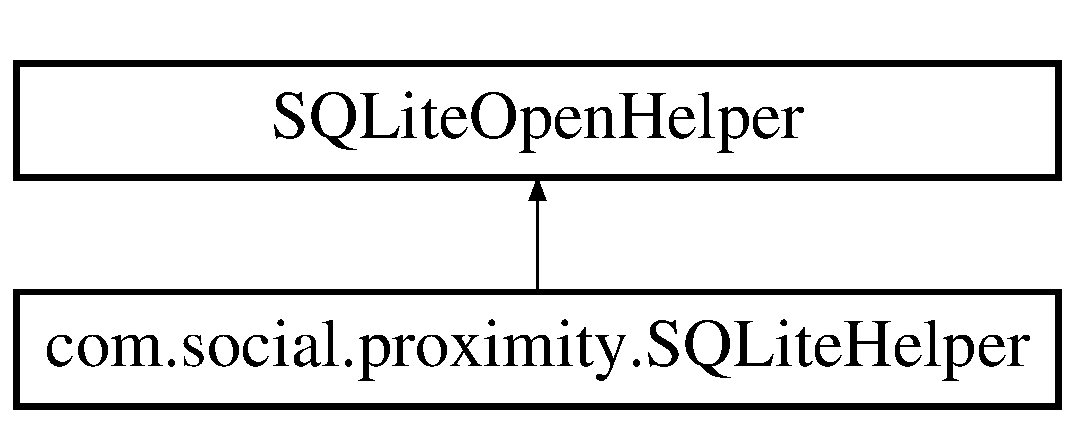
\includegraphics[height=2.000000cm]{classcom_1_1social_1_1proximity_1_1_s_q_lite_helper}
\end{center}
\end{figure}
\subsection*{Public Member Functions}
\begin{DoxyCompactItemize}
\item 
\hyperlink{classcom_1_1social_1_1proximity_1_1_s_q_lite_helper_a4bda85b0b433c8670f2ec11706fdbf53}{S\+Q\+Lite\+Helper} (Context context)
\item 
void \hyperlink{classcom_1_1social_1_1proximity_1_1_s_q_lite_helper_a1487315f51cd3c1400563bc1737aa5dc}{on\+Create} (S\+Q\+Lite\+Database data\+Base)
\item 
void \hyperlink{classcom_1_1social_1_1proximity_1_1_s_q_lite_helper_a5d049ccb92e3385123eab21ea55a25fc}{on\+Upgrade} (S\+Q\+Lite\+Database data\+Base, int old\+Version, int new\+Version)
\end{DoxyCompactItemize}
\subsection*{Static Public Attributes}
\begin{DoxyCompactItemize}
\item 
static final String \hyperlink{classcom_1_1social_1_1proximity_1_1_s_q_lite_helper_a5826d20868ba7e0d81bfb3de783baf07}{T\+A\+B\+L\+E\+\_\+\+B\+T\+D\+E\+V\+I\+C\+E} = \char`\"{}btdevices\char`\"{}
\item 
static final String \hyperlink{classcom_1_1social_1_1proximity_1_1_s_q_lite_helper_a7a34326231133feb3823c4fa9284e729}{T\+A\+B\+L\+E\+\_\+\+B\+T\+D\+E\+V\+I\+C\+E\+E\+N\+C\+O\+U\+N\+T\+E\+R\+D\+U\+R\+A\+T\+I\+O\+N} = \char`\"{}btdevice\+\_\+encounterduration\char`\"{}
\item 
static final String \hyperlink{classcom_1_1social_1_1proximity_1_1_s_q_lite_helper_a7d315c0f15f61c01bac3aba824e6bbce}{T\+A\+B\+L\+E\+\_\+\+B\+T\+D\+E\+V\+I\+C\+E\+A\+V\+E\+R\+A\+G\+E\+E\+N\+C\+O\+U\+N\+T\+E\+R\+D\+U\+R\+A\+T\+I\+O\+N} = \char`\"{}btdevice\+\_\+averageencounterduration\char`\"{}
\item 
static final String \hyperlink{classcom_1_1social_1_1proximity_1_1_s_q_lite_helper_a151e3b34b78b984d2dde9c2ea58d549e}{T\+A\+B\+L\+E\+\_\+\+B\+T\+D\+E\+V\+I\+C\+E\+S\+O\+C\+I\+A\+L\+W\+E\+I\+G\+H\+T} = \char`\"{}btdevice\+\_\+socialweight\char`\"{}
\item 
static final String \hyperlink{classcom_1_1social_1_1proximity_1_1_s_q_lite_helper_ae0e5a93fedecddb46106b02b939e4601}{C\+O\+L\+U\+M\+N\+\_\+\+I\+D} = \char`\"{}\+\_\+id\char`\"{}
\item 
static final String \hyperlink{classcom_1_1social_1_1proximity_1_1_s_q_lite_helper_a24fb4cdd15815c0527eecadbb7fb5f12}{C\+O\+L\+U\+M\+N\+\_\+\+B\+T\+D\+E\+V\+\_\+\+M\+A\+C\+\_\+\+A\+D\+D\+R\+E\+S\+S} = \char`\"{}dev\+Bt\+Mac\+Add\char`\"{}
\item 
static final String \hyperlink{classcom_1_1social_1_1proximity_1_1_s_q_lite_helper_af43c8ca7e0fb3301d929481e93a6b449}{C\+O\+L\+U\+M\+N\+\_\+\+B\+T\+D\+E\+V\+\_\+\+N\+A\+M\+E} = \char`\"{}dev\+Name\char`\"{}
\item 
static final String \hyperlink{classcom_1_1social_1_1proximity_1_1_s_q_lite_helper_aa1144aca9189f5fec6b5e19ac5887e89}{C\+O\+L\+U\+M\+N\+\_\+\+B\+T\+D\+E\+V\+\_\+\+E\+N\+C\+O\+U\+N\+T\+E\+R\+S\+T\+A\+R\+T} = \char`\"{}dev\+Encounter\+Start\char`\"{}
\item 
static final String \hyperlink{classcom_1_1social_1_1proximity_1_1_s_q_lite_helper_a868a3972f2b8525dc6f9405ced3646a1}{C\+O\+L\+U\+M\+N\+\_\+\+B\+T\+D\+E\+V\+\_\+\+E\+N\+C\+O\+U\+N\+T\+E\+R\+D\+U\+R\+A\+T\+I\+O\+N\+\_\+\+S\+L\+O\+T1} = \char`\"{}dev\+Encounter\+Duration\+\_\+slot1\char`\"{}
\item 
static final String \hyperlink{classcom_1_1social_1_1proximity_1_1_s_q_lite_helper_a5c34a24458903b46541f5f6464fc5158}{C\+O\+L\+U\+M\+N\+\_\+\+B\+T\+D\+E\+V\+\_\+\+E\+N\+C\+O\+U\+N\+T\+E\+R\+D\+U\+R\+A\+T\+I\+O\+N\+\_\+\+S\+L\+O\+T2} = \char`\"{}dev\+Encounter\+Duration\+\_\+slot2\char`\"{}
\item 
static final String \hyperlink{classcom_1_1social_1_1proximity_1_1_s_q_lite_helper_ab17d2432d4955f20c86940a793b391d7}{C\+O\+L\+U\+M\+N\+\_\+\+B\+T\+D\+E\+V\+\_\+\+E\+N\+C\+O\+U\+N\+T\+E\+R\+D\+U\+R\+A\+T\+I\+O\+N\+\_\+\+S\+L\+O\+T3} = \char`\"{}dev\+Encounter\+Duration\+\_\+slot3\char`\"{}
\item 
static final String \hyperlink{classcom_1_1social_1_1proximity_1_1_s_q_lite_helper_a09a133f4146b7472d28124a3f783b7b9}{C\+O\+L\+U\+M\+N\+\_\+\+B\+T\+D\+E\+V\+\_\+\+E\+N\+C\+O\+U\+N\+T\+E\+R\+D\+U\+R\+A\+T\+I\+O\+N\+\_\+\+S\+L\+O\+T4} = \char`\"{}dev\+Encounter\+Duration\+\_\+slot4\char`\"{}
\item 
static final String \hyperlink{classcom_1_1social_1_1proximity_1_1_s_q_lite_helper_ac3454a41a32eb6c763bcc1b4730485a5}{C\+O\+L\+U\+M\+N\+\_\+\+B\+T\+D\+E\+V\+\_\+\+E\+N\+C\+O\+U\+N\+T\+E\+R\+D\+U\+R\+A\+T\+I\+O\+N\+\_\+\+S\+L\+O\+T5} = \char`\"{}dev\+Encounter\+Duration\+\_\+slot5\char`\"{}
\item 
static final String \hyperlink{classcom_1_1social_1_1proximity_1_1_s_q_lite_helper_a71abceb54b8d7f3d2cd4029fc2216b27}{C\+O\+L\+U\+M\+N\+\_\+\+B\+T\+D\+E\+V\+\_\+\+E\+N\+C\+O\+U\+N\+T\+E\+R\+D\+U\+R\+A\+T\+I\+O\+N\+\_\+\+S\+L\+O\+T6} = \char`\"{}dev\+Encounter\+Duration\+\_\+slot6\char`\"{}
\item 
static final String \hyperlink{classcom_1_1social_1_1proximity_1_1_s_q_lite_helper_a067a13e5269073d37f02fd3ed84d9f29}{C\+O\+L\+U\+M\+N\+\_\+\+B\+T\+D\+E\+V\+\_\+\+E\+N\+C\+O\+U\+N\+T\+E\+R\+D\+U\+R\+A\+T\+I\+O\+N\+\_\+\+S\+L\+O\+T7} = \char`\"{}dev\+Encounter\+Duration\+\_\+slot7\char`\"{}
\item 
static final String \hyperlink{classcom_1_1social_1_1proximity_1_1_s_q_lite_helper_af64db8c92d3946598301b604c023cedf}{C\+O\+L\+U\+M\+N\+\_\+\+B\+T\+D\+E\+V\+\_\+\+E\+N\+C\+O\+U\+N\+T\+E\+R\+D\+U\+R\+A\+T\+I\+O\+N\+\_\+\+S\+L\+O\+T8} = \char`\"{}dev\+Encounter\+Duration\+\_\+slot8\char`\"{}
\item 
static final String \hyperlink{classcom_1_1social_1_1proximity_1_1_s_q_lite_helper_ac158849584082cfe70d33c70cedf4755}{C\+O\+L\+U\+M\+N\+\_\+\+B\+T\+D\+E\+V\+\_\+\+E\+N\+C\+O\+U\+N\+T\+E\+R\+D\+U\+R\+A\+T\+I\+O\+N\+\_\+\+S\+L\+O\+T9} = \char`\"{}dev\+Encounter\+Duration\+\_\+slot9\char`\"{}
\item 
static final String \hyperlink{classcom_1_1social_1_1proximity_1_1_s_q_lite_helper_a5ba0cd9a977e655f9d6989b39d0aa8b4}{C\+O\+L\+U\+M\+N\+\_\+\+B\+T\+D\+E\+V\+\_\+\+E\+N\+C\+O\+U\+N\+T\+E\+R\+D\+U\+R\+A\+T\+I\+O\+N\+\_\+\+S\+L\+O\+T10} = \char`\"{}dev\+Encounter\+Duration\+\_\+slot10\char`\"{}
\item 
static final String \hyperlink{classcom_1_1social_1_1proximity_1_1_s_q_lite_helper_a3ce051a1a793dab86096dc134f868209}{C\+O\+L\+U\+M\+N\+\_\+\+B\+T\+D\+E\+V\+\_\+\+E\+N\+C\+O\+U\+N\+T\+E\+R\+D\+U\+R\+A\+T\+I\+O\+N\+\_\+\+S\+L\+O\+T11} = \char`\"{}dev\+Encounter\+Duration\+\_\+slot11\char`\"{}
\item 
static final String \hyperlink{classcom_1_1social_1_1proximity_1_1_s_q_lite_helper_a246ee25c1f15c42957c92bfa5ee09c7c}{C\+O\+L\+U\+M\+N\+\_\+\+B\+T\+D\+E\+V\+\_\+\+E\+N\+C\+O\+U\+N\+T\+E\+R\+D\+U\+R\+A\+T\+I\+O\+N\+\_\+\+S\+L\+O\+T12} = \char`\"{}dev\+Encounter\+Duration\+\_\+slot12\char`\"{}
\item 
static final String \hyperlink{classcom_1_1social_1_1proximity_1_1_s_q_lite_helper_a9480c974d7f0ef4045ca4c34d9af46b6}{C\+O\+L\+U\+M\+N\+\_\+\+B\+T\+D\+E\+V\+\_\+\+E\+N\+C\+O\+U\+N\+T\+E\+R\+D\+U\+R\+A\+T\+I\+O\+N\+\_\+\+S\+L\+O\+T13} = \char`\"{}dev\+Encounter\+Duration\+\_\+slot13\char`\"{}
\item 
static final String \hyperlink{classcom_1_1social_1_1proximity_1_1_s_q_lite_helper_a1dcbfded30adb9b942ba4e81400ee4cf}{C\+O\+L\+U\+M\+N\+\_\+\+B\+T\+D\+E\+V\+\_\+\+E\+N\+C\+O\+U\+N\+T\+E\+R\+D\+U\+R\+A\+T\+I\+O\+N\+\_\+\+S\+L\+O\+T14} = \char`\"{}dev\+Encounter\+Duration\+\_\+slot14\char`\"{}
\item 
static final String \hyperlink{classcom_1_1social_1_1proximity_1_1_s_q_lite_helper_a20ffddb39e9b7a0de16c22e97a1fe59e}{C\+O\+L\+U\+M\+N\+\_\+\+B\+T\+D\+E\+V\+\_\+\+E\+N\+C\+O\+U\+N\+T\+E\+R\+D\+U\+R\+A\+T\+I\+O\+N\+\_\+\+S\+L\+O\+T15} = \char`\"{}dev\+Encounter\+Duration\+\_\+slot15\char`\"{}
\item 
static final String \hyperlink{classcom_1_1social_1_1proximity_1_1_s_q_lite_helper_a17332b2dcfbf24bac890a6938b985e07}{C\+O\+L\+U\+M\+N\+\_\+\+B\+T\+D\+E\+V\+\_\+\+E\+N\+C\+O\+U\+N\+T\+E\+R\+D\+U\+R\+A\+T\+I\+O\+N\+\_\+\+S\+L\+O\+T16} = \char`\"{}dev\+Encounter\+Duration\+\_\+slot16\char`\"{}
\item 
static final String \hyperlink{classcom_1_1social_1_1proximity_1_1_s_q_lite_helper_ad89f48a90c002e224b42a61c53a1646c}{C\+O\+L\+U\+M\+N\+\_\+\+B\+T\+D\+E\+V\+\_\+\+E\+N\+C\+O\+U\+N\+T\+E\+R\+D\+U\+R\+A\+T\+I\+O\+N\+\_\+\+S\+L\+O\+T17} = \char`\"{}dev\+Encounter\+Duration\+\_\+slot17\char`\"{}
\item 
static final String \hyperlink{classcom_1_1social_1_1proximity_1_1_s_q_lite_helper_a31c1917e141416f90f40b134635332ac}{C\+O\+L\+U\+M\+N\+\_\+\+B\+T\+D\+E\+V\+\_\+\+E\+N\+C\+O\+U\+N\+T\+E\+R\+D\+U\+R\+A\+T\+I\+O\+N\+\_\+\+S\+L\+O\+T18} = \char`\"{}dev\+Encounter\+Duration\+\_\+slot18\char`\"{}
\item 
static final String \hyperlink{classcom_1_1social_1_1proximity_1_1_s_q_lite_helper_a7566bf6b0339022bbd22a2bf01c491ed}{C\+O\+L\+U\+M\+N\+\_\+\+B\+T\+D\+E\+V\+\_\+\+E\+N\+C\+O\+U\+N\+T\+E\+R\+D\+U\+R\+A\+T\+I\+O\+N\+\_\+\+S\+L\+O\+T19} = \char`\"{}dev\+Encounter\+Duration\+\_\+slot19\char`\"{}
\item 
static final String \hyperlink{classcom_1_1social_1_1proximity_1_1_s_q_lite_helper_a30462676920857a1e2532cccab8ec3c4}{C\+O\+L\+U\+M\+N\+\_\+\+B\+T\+D\+E\+V\+\_\+\+E\+N\+C\+O\+U\+N\+T\+E\+R\+D\+U\+R\+A\+T\+I\+O\+N\+\_\+\+S\+L\+O\+T20} = \char`\"{}dev\+Encounter\+Duration\+\_\+slot20\char`\"{}
\item 
static final String \hyperlink{classcom_1_1social_1_1proximity_1_1_s_q_lite_helper_ac6c1e28fea294c28cbd5523f8b606f96}{C\+O\+L\+U\+M\+N\+\_\+\+B\+T\+D\+E\+V\+\_\+\+E\+N\+C\+O\+U\+N\+T\+E\+R\+D\+U\+R\+A\+T\+I\+O\+N\+\_\+\+S\+L\+O\+T21} = \char`\"{}dev\+Encounter\+Duration\+\_\+slot21\char`\"{}
\item 
static final String \hyperlink{classcom_1_1social_1_1proximity_1_1_s_q_lite_helper_a2d60f22417a7633262ad4a042ab98d96}{C\+O\+L\+U\+M\+N\+\_\+\+B\+T\+D\+E\+V\+\_\+\+E\+N\+C\+O\+U\+N\+T\+E\+R\+D\+U\+R\+A\+T\+I\+O\+N\+\_\+\+S\+L\+O\+T22} = \char`\"{}dev\+Encounter\+Duration\+\_\+slot22\char`\"{}
\item 
static final String \hyperlink{classcom_1_1social_1_1proximity_1_1_s_q_lite_helper_a37c71effb88d2a7da8cfe2301ea5b777}{C\+O\+L\+U\+M\+N\+\_\+\+B\+T\+D\+E\+V\+\_\+\+E\+N\+C\+O\+U\+N\+T\+E\+R\+D\+U\+R\+A\+T\+I\+O\+N\+\_\+\+S\+L\+O\+T23} = \char`\"{}dev\+Encounter\+Duration\+\_\+slot23\char`\"{}
\item 
static final String \hyperlink{classcom_1_1social_1_1proximity_1_1_s_q_lite_helper_ac314cf6fbe854832579bf6de4bcb17f0}{C\+O\+L\+U\+M\+N\+\_\+\+B\+T\+D\+E\+V\+\_\+\+E\+N\+C\+O\+U\+N\+T\+E\+R\+D\+U\+R\+A\+T\+I\+O\+N\+\_\+\+S\+L\+O\+T24} = \char`\"{}dev\+Encounter\+Duration\+\_\+slot24\char`\"{}
\item 
static final String \hyperlink{classcom_1_1social_1_1proximity_1_1_s_q_lite_helper_a3b3e9cdce16dfd979199820bb685a105}{C\+O\+L\+U\+M\+N\+\_\+\+B\+T\+D\+E\+V\+\_\+\+A\+V\+G\+E\+N\+C\+O\+U\+N\+T\+E\+R\+D\+U\+R\+A\+T\+I\+O\+N\+\_\+\+S\+L\+O\+T1} = \char`\"{}dev\+Avg\+Encounter\+Duration\+\_\+slot1\char`\"{}
\item 
static final String \hyperlink{classcom_1_1social_1_1proximity_1_1_s_q_lite_helper_a14c609ceff4a243797ac0ed38180c76b}{C\+O\+L\+U\+M\+N\+\_\+\+B\+T\+D\+E\+V\+\_\+\+A\+V\+G\+E\+N\+C\+O\+U\+N\+T\+E\+R\+D\+U\+R\+A\+T\+I\+O\+N\+\_\+\+S\+L\+O\+T2} = \char`\"{}dev\+Avg\+Encounter\+Duration\+\_\+slot2\char`\"{}
\item 
static final String \hyperlink{classcom_1_1social_1_1proximity_1_1_s_q_lite_helper_ac9ee299066e1659d2f00c7ac7b070c01}{C\+O\+L\+U\+M\+N\+\_\+\+B\+T\+D\+E\+V\+\_\+\+A\+V\+G\+E\+N\+C\+O\+U\+N\+T\+E\+R\+D\+U\+R\+A\+T\+I\+O\+N\+\_\+\+S\+L\+O\+T3} = \char`\"{}dev\+Avg\+Encounter\+Duration\+\_\+slot3\char`\"{}
\item 
static final String \hyperlink{classcom_1_1social_1_1proximity_1_1_s_q_lite_helper_a747c8f6e90116d66c055fdbaba96d56e}{C\+O\+L\+U\+M\+N\+\_\+\+B\+T\+D\+E\+V\+\_\+\+A\+V\+G\+E\+N\+C\+O\+U\+N\+T\+E\+R\+D\+U\+R\+A\+T\+I\+O\+N\+\_\+\+S\+L\+O\+T4} = \char`\"{}dev\+Avg\+Encounter\+Duration\+\_\+slot4\char`\"{}
\item 
static final String \hyperlink{classcom_1_1social_1_1proximity_1_1_s_q_lite_helper_a32dd31dc2a2bda82dd9673a33a2e4aac}{C\+O\+L\+U\+M\+N\+\_\+\+B\+T\+D\+E\+V\+\_\+\+A\+V\+G\+E\+N\+C\+O\+U\+N\+T\+E\+R\+D\+U\+R\+A\+T\+I\+O\+N\+\_\+\+S\+L\+O\+T5} = \char`\"{}dev\+Avg\+Encounter\+Duration\+\_\+slot5\char`\"{}
\item 
static final String \hyperlink{classcom_1_1social_1_1proximity_1_1_s_q_lite_helper_a86b01514c7e56288d280557e605f5d7b}{C\+O\+L\+U\+M\+N\+\_\+\+B\+T\+D\+E\+V\+\_\+\+A\+V\+G\+E\+N\+C\+O\+U\+N\+T\+E\+R\+D\+U\+R\+A\+T\+I\+O\+N\+\_\+\+S\+L\+O\+T6} = \char`\"{}dev\+Avg\+Encounter\+Duration\+\_\+slot6\char`\"{}
\item 
static final String \hyperlink{classcom_1_1social_1_1proximity_1_1_s_q_lite_helper_a7ead17ba779351a033117f59e833b2fe}{C\+O\+L\+U\+M\+N\+\_\+\+B\+T\+D\+E\+V\+\_\+\+A\+V\+G\+E\+N\+C\+O\+U\+N\+T\+E\+R\+D\+U\+R\+A\+T\+I\+O\+N\+\_\+\+S\+L\+O\+T7} = \char`\"{}dev\+Avg\+Encounter\+Duration\+\_\+slot7\char`\"{}
\item 
static final String \hyperlink{classcom_1_1social_1_1proximity_1_1_s_q_lite_helper_a15bba1730515628bc4aff17ec1d8c9c4}{C\+O\+L\+U\+M\+N\+\_\+\+B\+T\+D\+E\+V\+\_\+\+A\+V\+G\+E\+N\+C\+O\+U\+N\+T\+E\+R\+D\+U\+R\+A\+T\+I\+O\+N\+\_\+\+S\+L\+O\+T8} = \char`\"{}dev\+Avg\+Encounter\+Duration\+\_\+slot8\char`\"{}
\item 
static final String \hyperlink{classcom_1_1social_1_1proximity_1_1_s_q_lite_helper_a671f0ef4fc52b1a396356de9b080dd05}{C\+O\+L\+U\+M\+N\+\_\+\+B\+T\+D\+E\+V\+\_\+\+A\+V\+G\+E\+N\+C\+O\+U\+N\+T\+E\+R\+D\+U\+R\+A\+T\+I\+O\+N\+\_\+\+S\+L\+O\+T9} = \char`\"{}dev\+Avg\+Encounter\+Duration\+\_\+slot9\char`\"{}
\item 
static final String \hyperlink{classcom_1_1social_1_1proximity_1_1_s_q_lite_helper_a36ef1962f26aead1302bdd08da18fc76}{C\+O\+L\+U\+M\+N\+\_\+\+B\+T\+D\+E\+V\+\_\+\+A\+V\+G\+E\+N\+C\+O\+U\+N\+T\+E\+R\+D\+U\+R\+A\+T\+I\+O\+N\+\_\+\+S\+L\+O\+T10} = \char`\"{}dev\+Avg\+Encounter\+Duration\+\_\+slot10\char`\"{}
\item 
static final String \hyperlink{classcom_1_1social_1_1proximity_1_1_s_q_lite_helper_a5f9d6d711fdab1b4887213020b14908d}{C\+O\+L\+U\+M\+N\+\_\+\+B\+T\+D\+E\+V\+\_\+\+A\+V\+G\+E\+N\+C\+O\+U\+N\+T\+E\+R\+D\+U\+R\+A\+T\+I\+O\+N\+\_\+\+S\+L\+O\+T11} = \char`\"{}dev\+Avg\+Encounter\+Duration\+\_\+slot11\char`\"{}
\item 
static final String \hyperlink{classcom_1_1social_1_1proximity_1_1_s_q_lite_helper_a33f2bcc11870df8e8f78ca94d44c870a}{C\+O\+L\+U\+M\+N\+\_\+\+B\+T\+D\+E\+V\+\_\+\+A\+V\+G\+E\+N\+C\+O\+U\+N\+T\+E\+R\+D\+U\+R\+A\+T\+I\+O\+N\+\_\+\+S\+L\+O\+T12} = \char`\"{}dev\+Avg\+Encounter\+Duration\+\_\+slot12\char`\"{}
\item 
static final String \hyperlink{classcom_1_1social_1_1proximity_1_1_s_q_lite_helper_a60029078266511cdbba0b2b022ac3319}{C\+O\+L\+U\+M\+N\+\_\+\+B\+T\+D\+E\+V\+\_\+\+A\+V\+G\+E\+N\+C\+O\+U\+N\+T\+E\+R\+D\+U\+R\+A\+T\+I\+O\+N\+\_\+\+S\+L\+O\+T13} = \char`\"{}dev\+Avg\+Encounter\+Duration\+\_\+slot13\char`\"{}
\item 
static final String \hyperlink{classcom_1_1social_1_1proximity_1_1_s_q_lite_helper_aff03ab377c605903c8ebab1716ef9616}{C\+O\+L\+U\+M\+N\+\_\+\+B\+T\+D\+E\+V\+\_\+\+A\+V\+G\+E\+N\+C\+O\+U\+N\+T\+E\+R\+D\+U\+R\+A\+T\+I\+O\+N\+\_\+\+S\+L\+O\+T14} = \char`\"{}dev\+Avg\+Encounter\+Duration\+\_\+slot14\char`\"{}
\item 
static final String \hyperlink{classcom_1_1social_1_1proximity_1_1_s_q_lite_helper_a030cda34629f2ebe573a5528561b6a2a}{C\+O\+L\+U\+M\+N\+\_\+\+B\+T\+D\+E\+V\+\_\+\+A\+V\+G\+E\+N\+C\+O\+U\+N\+T\+E\+R\+D\+U\+R\+A\+T\+I\+O\+N\+\_\+\+S\+L\+O\+T15} = \char`\"{}dev\+Avg\+Encounter\+Duration\+\_\+slot15\char`\"{}
\item 
static final String \hyperlink{classcom_1_1social_1_1proximity_1_1_s_q_lite_helper_af25494a3047b9adb89340e54d94a5dc3}{C\+O\+L\+U\+M\+N\+\_\+\+B\+T\+D\+E\+V\+\_\+\+A\+V\+G\+E\+N\+C\+O\+U\+N\+T\+E\+R\+D\+U\+R\+A\+T\+I\+O\+N\+\_\+\+S\+L\+O\+T16} = \char`\"{}dev\+Avg\+Encounter\+Duration\+\_\+slot16\char`\"{}
\item 
static final String \hyperlink{classcom_1_1social_1_1proximity_1_1_s_q_lite_helper_a9a7d1eb2eb2639091df2ea97e0dfeb7d}{C\+O\+L\+U\+M\+N\+\_\+\+B\+T\+D\+E\+V\+\_\+\+A\+V\+G\+E\+N\+C\+O\+U\+N\+T\+E\+R\+D\+U\+R\+A\+T\+I\+O\+N\+\_\+\+S\+L\+O\+T17} = \char`\"{}dev\+Avg\+Encounter\+Duration\+\_\+slot17\char`\"{}
\item 
static final String \hyperlink{classcom_1_1social_1_1proximity_1_1_s_q_lite_helper_a0eaf0df061e77b43c9856c68f685d483}{C\+O\+L\+U\+M\+N\+\_\+\+B\+T\+D\+E\+V\+\_\+\+A\+V\+G\+E\+N\+C\+O\+U\+N\+T\+E\+R\+D\+U\+R\+A\+T\+I\+O\+N\+\_\+\+S\+L\+O\+T18} = \char`\"{}dev\+Avg\+Encounter\+Duration\+\_\+slot18\char`\"{}
\item 
static final String \hyperlink{classcom_1_1social_1_1proximity_1_1_s_q_lite_helper_ab4ea60ed82b06142cb4474db3604c1a7}{C\+O\+L\+U\+M\+N\+\_\+\+B\+T\+D\+E\+V\+\_\+\+A\+V\+G\+E\+N\+C\+O\+U\+N\+T\+E\+R\+D\+U\+R\+A\+T\+I\+O\+N\+\_\+\+S\+L\+O\+T19} = \char`\"{}dev\+Avg\+Encounter\+Duration\+\_\+slot19\char`\"{}
\item 
static final String \hyperlink{classcom_1_1social_1_1proximity_1_1_s_q_lite_helper_af6ef170145c615192e7c40fd4a9a1428}{C\+O\+L\+U\+M\+N\+\_\+\+B\+T\+D\+E\+V\+\_\+\+A\+V\+G\+E\+N\+C\+O\+U\+N\+T\+E\+R\+D\+U\+R\+A\+T\+I\+O\+N\+\_\+\+S\+L\+O\+T20} = \char`\"{}dev\+Avg\+Encounter\+Duration\+\_\+slot20\char`\"{}
\item 
static final String \hyperlink{classcom_1_1social_1_1proximity_1_1_s_q_lite_helper_a83dd830a181065c409361f4be1fe74f4}{C\+O\+L\+U\+M\+N\+\_\+\+B\+T\+D\+E\+V\+\_\+\+A\+V\+G\+E\+N\+C\+O\+U\+N\+T\+E\+R\+D\+U\+R\+A\+T\+I\+O\+N\+\_\+\+S\+L\+O\+T21} = \char`\"{}dev\+Avg\+Encounter\+Duration\+\_\+slot21\char`\"{}
\item 
static final String \hyperlink{classcom_1_1social_1_1proximity_1_1_s_q_lite_helper_aca81099d56d66abb9f3ae813dbefcf75}{C\+O\+L\+U\+M\+N\+\_\+\+B\+T\+D\+E\+V\+\_\+\+A\+V\+G\+E\+N\+C\+O\+U\+N\+T\+E\+R\+D\+U\+R\+A\+T\+I\+O\+N\+\_\+\+S\+L\+O\+T22} = \char`\"{}dev\+Avg\+Encounter\+Duration\+\_\+slot22\char`\"{}
\item 
static final String \hyperlink{classcom_1_1social_1_1proximity_1_1_s_q_lite_helper_aed5dae0c9a3e1a846edc2c7892d4ab33}{C\+O\+L\+U\+M\+N\+\_\+\+B\+T\+D\+E\+V\+\_\+\+A\+V\+G\+E\+N\+C\+O\+U\+N\+T\+E\+R\+D\+U\+R\+A\+T\+I\+O\+N\+\_\+\+S\+L\+O\+T23} = \char`\"{}dev\+Avg\+Encounter\+Duration\+\_\+slot23\char`\"{}
\item 
static final String \hyperlink{classcom_1_1social_1_1proximity_1_1_s_q_lite_helper_a6a0c6049d9504d4a7e49b192b5c90a69}{C\+O\+L\+U\+M\+N\+\_\+\+B\+T\+D\+E\+V\+\_\+\+A\+V\+G\+E\+N\+C\+O\+U\+N\+T\+E\+R\+D\+U\+R\+A\+T\+I\+O\+N\+\_\+\+S\+L\+O\+T24} = \char`\"{}dev\+Avg\+Encounter\+Duration\+\_\+slot24\char`\"{}
\item 
static final String \hyperlink{classcom_1_1social_1_1proximity_1_1_s_q_lite_helper_adfc6730a2f078bba8844101b011fc377}{C\+O\+L\+U\+M\+N\+\_\+\+B\+T\+D\+E\+V\+\_\+\+S\+O\+C\+I\+A\+L\+W\+E\+I\+G\+H\+T\+\_\+\+S\+L\+O\+T1} = \char`\"{}dev\+Social\+Weight\+\_\+slot1\char`\"{}
\item 
static final String \hyperlink{classcom_1_1social_1_1proximity_1_1_s_q_lite_helper_af21ae06cc954eb56b05dabcb682e3571}{C\+O\+L\+U\+M\+N\+\_\+\+B\+T\+D\+E\+V\+\_\+\+S\+O\+C\+I\+A\+L\+W\+E\+I\+G\+H\+T\+\_\+\+S\+L\+O\+T2} = \char`\"{}dev\+Social\+Weight\+\_\+slot2\char`\"{}
\item 
static final String \hyperlink{classcom_1_1social_1_1proximity_1_1_s_q_lite_helper_af648dcc55968d0857315b6f1e2ea7bd5}{C\+O\+L\+U\+M\+N\+\_\+\+B\+T\+D\+E\+V\+\_\+\+S\+O\+C\+I\+A\+L\+W\+E\+I\+G\+H\+T\+\_\+\+S\+L\+O\+T3} = \char`\"{}dev\+Social\+Weight\+\_\+slot3\char`\"{}
\item 
static final String \hyperlink{classcom_1_1social_1_1proximity_1_1_s_q_lite_helper_a71c55d8a651651735eb03c39bfd33ffe}{C\+O\+L\+U\+M\+N\+\_\+\+B\+T\+D\+E\+V\+\_\+\+S\+O\+C\+I\+A\+L\+W\+E\+I\+G\+H\+T\+\_\+\+S\+L\+O\+T4} = \char`\"{}dev\+Social\+Weight\+\_\+slot4\char`\"{}
\item 
static final String \hyperlink{classcom_1_1social_1_1proximity_1_1_s_q_lite_helper_acf03bd9df5a5d9aff1736e8279f0c18f}{C\+O\+L\+U\+M\+N\+\_\+\+B\+T\+D\+E\+V\+\_\+\+S\+O\+C\+I\+A\+L\+W\+E\+I\+G\+H\+T\+\_\+\+S\+L\+O\+T5} = \char`\"{}dev\+Social\+Weight\+\_\+slot5\char`\"{}
\item 
static final String \hyperlink{classcom_1_1social_1_1proximity_1_1_s_q_lite_helper_aba87fe71d289765dc72304a6474eb21b}{C\+O\+L\+U\+M\+N\+\_\+\+B\+T\+D\+E\+V\+\_\+\+S\+O\+C\+I\+A\+L\+W\+E\+I\+G\+H\+T\+\_\+\+S\+L\+O\+T6} = \char`\"{}dev\+Social\+Weight\+\_\+slot6\char`\"{}
\item 
static final String \hyperlink{classcom_1_1social_1_1proximity_1_1_s_q_lite_helper_af4e04fe6db4068a7bc14dd98ceb4ad46}{C\+O\+L\+U\+M\+N\+\_\+\+B\+T\+D\+E\+V\+\_\+\+S\+O\+C\+I\+A\+L\+W\+E\+I\+G\+H\+T\+\_\+\+S\+L\+O\+T7} = \char`\"{}dev\+Social\+Weight\+\_\+slot7\char`\"{}
\item 
static final String \hyperlink{classcom_1_1social_1_1proximity_1_1_s_q_lite_helper_a53e97bb3b563d46746140235cf0f2db0}{C\+O\+L\+U\+M\+N\+\_\+\+B\+T\+D\+E\+V\+\_\+\+S\+O\+C\+I\+A\+L\+W\+E\+I\+G\+H\+T\+\_\+\+S\+L\+O\+T8} = \char`\"{}dev\+Social\+Weight\+\_\+slot8\char`\"{}
\item 
static final String \hyperlink{classcom_1_1social_1_1proximity_1_1_s_q_lite_helper_a1fe7a2cfa003028ed870c3d9fd9c68fa}{C\+O\+L\+U\+M\+N\+\_\+\+B\+T\+D\+E\+V\+\_\+\+S\+O\+C\+I\+A\+L\+W\+E\+I\+G\+H\+T\+\_\+\+S\+L\+O\+T9} = \char`\"{}dev\+Social\+Weight\+\_\+slot9\char`\"{}
\item 
static final String \hyperlink{classcom_1_1social_1_1proximity_1_1_s_q_lite_helper_a9f98a31fa6165552da5bbdf5933728cc}{C\+O\+L\+U\+M\+N\+\_\+\+B\+T\+D\+E\+V\+\_\+\+S\+O\+C\+I\+A\+L\+W\+E\+I\+G\+H\+T\+\_\+\+S\+L\+O\+T10} = \char`\"{}dev\+Social\+Weight\+\_\+slot10\char`\"{}
\item 
static final String \hyperlink{classcom_1_1social_1_1proximity_1_1_s_q_lite_helper_aa729ff0739a99c0ba71ab1494d138c67}{C\+O\+L\+U\+M\+N\+\_\+\+B\+T\+D\+E\+V\+\_\+\+S\+O\+C\+I\+A\+L\+W\+E\+I\+G\+H\+T\+\_\+\+S\+L\+O\+T11} = \char`\"{}dev\+Social\+Weight\+\_\+slot11\char`\"{}
\item 
static final String \hyperlink{classcom_1_1social_1_1proximity_1_1_s_q_lite_helper_ac8e1cb1c089ecd9de0233e4779235c66}{C\+O\+L\+U\+M\+N\+\_\+\+B\+T\+D\+E\+V\+\_\+\+S\+O\+C\+I\+A\+L\+W\+E\+I\+G\+H\+T\+\_\+\+S\+L\+O\+T12} = \char`\"{}dev\+Social\+Weight\+\_\+slot12\char`\"{}
\item 
static final String \hyperlink{classcom_1_1social_1_1proximity_1_1_s_q_lite_helper_a2d87a2fd701e0b61cadf163594a3bec1}{C\+O\+L\+U\+M\+N\+\_\+\+B\+T\+D\+E\+V\+\_\+\+S\+O\+C\+I\+A\+L\+W\+E\+I\+G\+H\+T\+\_\+\+S\+L\+O\+T13} = \char`\"{}dev\+Social\+Weight\+\_\+slot13\char`\"{}
\item 
static final String \hyperlink{classcom_1_1social_1_1proximity_1_1_s_q_lite_helper_a3e7b695f8efbfc00b21504aa02d7d59f}{C\+O\+L\+U\+M\+N\+\_\+\+B\+T\+D\+E\+V\+\_\+\+S\+O\+C\+I\+A\+L\+W\+E\+I\+G\+H\+T\+\_\+\+S\+L\+O\+T14} = \char`\"{}dev\+Social\+Weight\+\_\+slot14\char`\"{}
\item 
static final String \hyperlink{classcom_1_1social_1_1proximity_1_1_s_q_lite_helper_ad0a80f64e98863ff57a4cf8f9a113766}{C\+O\+L\+U\+M\+N\+\_\+\+B\+T\+D\+E\+V\+\_\+\+S\+O\+C\+I\+A\+L\+W\+E\+I\+G\+H\+T\+\_\+\+S\+L\+O\+T15} = \char`\"{}dev\+Social\+Weight\+\_\+slot15\char`\"{}
\item 
static final String \hyperlink{classcom_1_1social_1_1proximity_1_1_s_q_lite_helper_aca5c6c9e141b90bd7e730c65f93849a0}{C\+O\+L\+U\+M\+N\+\_\+\+B\+T\+D\+E\+V\+\_\+\+S\+O\+C\+I\+A\+L\+W\+E\+I\+G\+H\+T\+\_\+\+S\+L\+O\+T16} = \char`\"{}dev\+Social\+Weight\+\_\+slot16\char`\"{}
\item 
static final String \hyperlink{classcom_1_1social_1_1proximity_1_1_s_q_lite_helper_a444273fa0ffa682c5b0d789d1e91725a}{C\+O\+L\+U\+M\+N\+\_\+\+B\+T\+D\+E\+V\+\_\+\+S\+O\+C\+I\+A\+L\+W\+E\+I\+G\+H\+T\+\_\+\+S\+L\+O\+T17} = \char`\"{}dev\+Social\+Weight\+\_\+slot17\char`\"{}
\item 
static final String \hyperlink{classcom_1_1social_1_1proximity_1_1_s_q_lite_helper_a7440b69bf721bc1699d3f9b44760bb8a}{C\+O\+L\+U\+M\+N\+\_\+\+B\+T\+D\+E\+V\+\_\+\+S\+O\+C\+I\+A\+L\+W\+E\+I\+G\+H\+T\+\_\+\+S\+L\+O\+T18} = \char`\"{}dev\+Social\+Weight\+\_\+slot18\char`\"{}
\item 
static final String \hyperlink{classcom_1_1social_1_1proximity_1_1_s_q_lite_helper_a922ea6d87617bdd176083bff3c930e8c}{C\+O\+L\+U\+M\+N\+\_\+\+B\+T\+D\+E\+V\+\_\+\+S\+O\+C\+I\+A\+L\+W\+E\+I\+G\+H\+T\+\_\+\+S\+L\+O\+T19} = \char`\"{}dev\+Social\+Weight\+\_\+slot19\char`\"{}
\item 
static final String \hyperlink{classcom_1_1social_1_1proximity_1_1_s_q_lite_helper_afa9d11d75fd116d78e17cc13eb917f84}{C\+O\+L\+U\+M\+N\+\_\+\+B\+T\+D\+E\+V\+\_\+\+S\+O\+C\+I\+A\+L\+W\+E\+I\+G\+H\+T\+\_\+\+S\+L\+O\+T20} = \char`\"{}dev\+Social\+Weight\+\_\+slot20\char`\"{}
\item 
static final String \hyperlink{classcom_1_1social_1_1proximity_1_1_s_q_lite_helper_ad8bc64cd84ccb74a9511ac6964499e55}{C\+O\+L\+U\+M\+N\+\_\+\+B\+T\+D\+E\+V\+\_\+\+S\+O\+C\+I\+A\+L\+W\+E\+I\+G\+H\+T\+\_\+\+S\+L\+O\+T21} = \char`\"{}dev\+Social\+Weight\+\_\+slot21\char`\"{}
\item 
static final String \hyperlink{classcom_1_1social_1_1proximity_1_1_s_q_lite_helper_ad4c99b480a345c22fc43bc298c43a2ac}{C\+O\+L\+U\+M\+N\+\_\+\+B\+T\+D\+E\+V\+\_\+\+S\+O\+C\+I\+A\+L\+W\+E\+I\+G\+H\+T\+\_\+\+S\+L\+O\+T22} = \char`\"{}dev\+Social\+Weight\+\_\+slot22\char`\"{}
\item 
static final String \hyperlink{classcom_1_1social_1_1proximity_1_1_s_q_lite_helper_a52e7f4d707bc6b90bade10abaee77851}{C\+O\+L\+U\+M\+N\+\_\+\+B\+T\+D\+E\+V\+\_\+\+S\+O\+C\+I\+A\+L\+W\+E\+I\+G\+H\+T\+\_\+\+S\+L\+O\+T23} = \char`\"{}dev\+Social\+Weight\+\_\+slot23\char`\"{}
\item 
static final String \hyperlink{classcom_1_1social_1_1proximity_1_1_s_q_lite_helper_adf47474141453dfa6343838e2f69b0ea}{C\+O\+L\+U\+M\+N\+\_\+\+B\+T\+D\+E\+V\+\_\+\+S\+O\+C\+I\+A\+L\+W\+E\+I\+G\+H\+T\+\_\+\+S\+L\+O\+T24} = \char`\"{}dev\+Social\+Weight\+\_\+slot24\char`\"{}
\end{DoxyCompactItemize}
\subsection*{Static Private Attributes}
\begin{DoxyCompactItemize}
\item 
static final String \hyperlink{classcom_1_1social_1_1proximity_1_1_s_q_lite_helper_a46aed568d90b22207e3c240e37de865b}{D\+A\+T\+A\+B\+A\+S\+E\+\_\+\+N\+A\+M\+E} = \char`\"{}database\char`\"{}
\item 
static final int \hyperlink{classcom_1_1social_1_1proximity_1_1_s_q_lite_helper_a7e5876fc2bc6861e6fbb1c84616dcd07}{D\+A\+T\+A\+B\+A\+S\+E\+\_\+\+V\+E\+R\+S\+I\+O\+N} = 2
\item 
static final String \hyperlink{classcom_1_1social_1_1proximity_1_1_s_q_lite_helper_a008345746681ebe4ff451e164809f343}{C\+R\+E\+A\+T\+E\+\_\+\+B\+T\+D\+E\+V\+I\+C\+E\+\_\+\+T\+A\+B\+L\+E}
\item 
static final String \hyperlink{classcom_1_1social_1_1proximity_1_1_s_q_lite_helper_aa47200bd55a879de8afff2709a50cc76}{C\+R\+E\+A\+T\+E\+\_\+\+B\+T\+D\+E\+V\+I\+C\+E\+E\+N\+C\+O\+U\+N\+T\+E\+R\+D\+U\+R\+A\+T\+I\+O\+N\+\_\+\+T\+A\+B\+L\+E}
\item 
static final String \hyperlink{classcom_1_1social_1_1proximity_1_1_s_q_lite_helper_ad6fd653f953e708728c7e84845208638}{C\+R\+E\+A\+T\+E\+\_\+\+B\+T\+D\+E\+V\+I\+C\+E\+A\+V\+E\+R\+A\+G\+E\+E\+N\+C\+O\+U\+N\+T\+E\+R\+D\+U\+R\+A\+T\+I\+O\+N\+\_\+\+T\+A\+B\+L\+E}
\item 
static final String \hyperlink{classcom_1_1social_1_1proximity_1_1_s_q_lite_helper_a2ffdca634cf057e96a94972b2e5704e4}{C\+R\+E\+A\+T\+E\+\_\+\+B\+T\+D\+E\+V\+I\+C\+E\+S\+O\+C\+I\+A\+L\+W\+E\+I\+G\+H\+T\+\_\+\+T\+A\+B\+L\+E}
\end{DoxyCompactItemize}


\subsection{Constructor \& Destructor Documentation}
\hypertarget{classcom_1_1social_1_1proximity_1_1_s_q_lite_helper_a4bda85b0b433c8670f2ec11706fdbf53}{}\index{com\+::social\+::proximity\+::\+S\+Q\+Lite\+Helper@{com\+::social\+::proximity\+::\+S\+Q\+Lite\+Helper}!S\+Q\+Lite\+Helper@{S\+Q\+Lite\+Helper}}
\index{S\+Q\+Lite\+Helper@{S\+Q\+Lite\+Helper}!com\+::social\+::proximity\+::\+S\+Q\+Lite\+Helper@{com\+::social\+::proximity\+::\+S\+Q\+Lite\+Helper}}
\subsubsection[{S\+Q\+Lite\+Helper(\+Context context)}]{\setlength{\rightskip}{0pt plus 5cm}com.\+social.\+proximity.\+S\+Q\+Lite\+Helper.\+S\+Q\+Lite\+Helper (
\begin{DoxyParamCaption}
\item[{Context}]{context}
\end{DoxyParamCaption}
)}\label{classcom_1_1social_1_1proximity_1_1_s_q_lite_helper_a4bda85b0b433c8670f2ec11706fdbf53}
\hyperlink{classcom_1_1social_1_1proximity_1_1_s_q_lite_helper}{S\+Q\+Lite\+Helper} constructor. 
\begin{DoxyParams}{Parameters}
{\em context} & The context which provides access to resources and specific classes of the application. \\
\hline
\end{DoxyParams}


\subsection{Member Function Documentation}
\hypertarget{classcom_1_1social_1_1proximity_1_1_s_q_lite_helper_a1487315f51cd3c1400563bc1737aa5dc}{}\index{com\+::social\+::proximity\+::\+S\+Q\+Lite\+Helper@{com\+::social\+::proximity\+::\+S\+Q\+Lite\+Helper}!on\+Create@{on\+Create}}
\index{on\+Create@{on\+Create}!com\+::social\+::proximity\+::\+S\+Q\+Lite\+Helper@{com\+::social\+::proximity\+::\+S\+Q\+Lite\+Helper}}
\subsubsection[{on\+Create(\+S\+Q\+Lite\+Database data\+Base)}]{\setlength{\rightskip}{0pt plus 5cm}void com.\+social.\+proximity.\+S\+Q\+Lite\+Helper.\+on\+Create (
\begin{DoxyParamCaption}
\item[{S\+Q\+Lite\+Database}]{data\+Base}
\end{DoxyParamCaption}
)}\label{classcom_1_1social_1_1proximity_1_1_s_q_lite_helper_a1487315f51cd3c1400563bc1737aa5dc}
\hypertarget{classcom_1_1social_1_1proximity_1_1_s_q_lite_helper_a5d049ccb92e3385123eab21ea55a25fc}{}\index{com\+::social\+::proximity\+::\+S\+Q\+Lite\+Helper@{com\+::social\+::proximity\+::\+S\+Q\+Lite\+Helper}!on\+Upgrade@{on\+Upgrade}}
\index{on\+Upgrade@{on\+Upgrade}!com\+::social\+::proximity\+::\+S\+Q\+Lite\+Helper@{com\+::social\+::proximity\+::\+S\+Q\+Lite\+Helper}}
\subsubsection[{on\+Upgrade(\+S\+Q\+Lite\+Database data\+Base, int old\+Version, int new\+Version)}]{\setlength{\rightskip}{0pt plus 5cm}void com.\+social.\+proximity.\+S\+Q\+Lite\+Helper.\+on\+Upgrade (
\begin{DoxyParamCaption}
\item[{S\+Q\+Lite\+Database}]{data\+Base, }
\item[{int}]{old\+Version, }
\item[{int}]{new\+Version}
\end{DoxyParamCaption}
)}\label{classcom_1_1social_1_1proximity_1_1_s_q_lite_helper_a5d049ccb92e3385123eab21ea55a25fc}


\subsection{Member Data Documentation}
\hypertarget{classcom_1_1social_1_1proximity_1_1_s_q_lite_helper_a3b3e9cdce16dfd979199820bb685a105}{}\index{com\+::social\+::proximity\+::\+S\+Q\+Lite\+Helper@{com\+::social\+::proximity\+::\+S\+Q\+Lite\+Helper}!C\+O\+L\+U\+M\+N\+\_\+\+B\+T\+D\+E\+V\+\_\+\+A\+V\+G\+E\+N\+C\+O\+U\+N\+T\+E\+R\+D\+U\+R\+A\+T\+I\+O\+N\+\_\+\+S\+L\+O\+T1@{C\+O\+L\+U\+M\+N\+\_\+\+B\+T\+D\+E\+V\+\_\+\+A\+V\+G\+E\+N\+C\+O\+U\+N\+T\+E\+R\+D\+U\+R\+A\+T\+I\+O\+N\+\_\+\+S\+L\+O\+T1}}
\index{C\+O\+L\+U\+M\+N\+\_\+\+B\+T\+D\+E\+V\+\_\+\+A\+V\+G\+E\+N\+C\+O\+U\+N\+T\+E\+R\+D\+U\+R\+A\+T\+I\+O\+N\+\_\+\+S\+L\+O\+T1@{C\+O\+L\+U\+M\+N\+\_\+\+B\+T\+D\+E\+V\+\_\+\+A\+V\+G\+E\+N\+C\+O\+U\+N\+T\+E\+R\+D\+U\+R\+A\+T\+I\+O\+N\+\_\+\+S\+L\+O\+T1}!com\+::social\+::proximity\+::\+S\+Q\+Lite\+Helper@{com\+::social\+::proximity\+::\+S\+Q\+Lite\+Helper}}
\subsubsection[{C\+O\+L\+U\+M\+N\+\_\+\+B\+T\+D\+E\+V\+\_\+\+A\+V\+G\+E\+N\+C\+O\+U\+N\+T\+E\+R\+D\+U\+R\+A\+T\+I\+O\+N\+\_\+\+S\+L\+O\+T1}]{\setlength{\rightskip}{0pt plus 5cm}final String com.\+social.\+proximity.\+S\+Q\+Lite\+Helper.\+C\+O\+L\+U\+M\+N\+\_\+\+B\+T\+D\+E\+V\+\_\+\+A\+V\+G\+E\+N\+C\+O\+U\+N\+T\+E\+R\+D\+U\+R\+A\+T\+I\+O\+N\+\_\+\+S\+L\+O\+T1 = \char`\"{}dev\+Avg\+Encounter\+Duration\+\_\+slot1\char`\"{}\hspace{0.3cm}{\ttfamily [static]}}\label{classcom_1_1social_1_1proximity_1_1_s_q_lite_helper_a3b3e9cdce16dfd979199820bb685a105}
\hypertarget{classcom_1_1social_1_1proximity_1_1_s_q_lite_helper_a36ef1962f26aead1302bdd08da18fc76}{}\index{com\+::social\+::proximity\+::\+S\+Q\+Lite\+Helper@{com\+::social\+::proximity\+::\+S\+Q\+Lite\+Helper}!C\+O\+L\+U\+M\+N\+\_\+\+B\+T\+D\+E\+V\+\_\+\+A\+V\+G\+E\+N\+C\+O\+U\+N\+T\+E\+R\+D\+U\+R\+A\+T\+I\+O\+N\+\_\+\+S\+L\+O\+T10@{C\+O\+L\+U\+M\+N\+\_\+\+B\+T\+D\+E\+V\+\_\+\+A\+V\+G\+E\+N\+C\+O\+U\+N\+T\+E\+R\+D\+U\+R\+A\+T\+I\+O\+N\+\_\+\+S\+L\+O\+T10}}
\index{C\+O\+L\+U\+M\+N\+\_\+\+B\+T\+D\+E\+V\+\_\+\+A\+V\+G\+E\+N\+C\+O\+U\+N\+T\+E\+R\+D\+U\+R\+A\+T\+I\+O\+N\+\_\+\+S\+L\+O\+T10@{C\+O\+L\+U\+M\+N\+\_\+\+B\+T\+D\+E\+V\+\_\+\+A\+V\+G\+E\+N\+C\+O\+U\+N\+T\+E\+R\+D\+U\+R\+A\+T\+I\+O\+N\+\_\+\+S\+L\+O\+T10}!com\+::social\+::proximity\+::\+S\+Q\+Lite\+Helper@{com\+::social\+::proximity\+::\+S\+Q\+Lite\+Helper}}
\subsubsection[{C\+O\+L\+U\+M\+N\+\_\+\+B\+T\+D\+E\+V\+\_\+\+A\+V\+G\+E\+N\+C\+O\+U\+N\+T\+E\+R\+D\+U\+R\+A\+T\+I\+O\+N\+\_\+\+S\+L\+O\+T10}]{\setlength{\rightskip}{0pt plus 5cm}final String com.\+social.\+proximity.\+S\+Q\+Lite\+Helper.\+C\+O\+L\+U\+M\+N\+\_\+\+B\+T\+D\+E\+V\+\_\+\+A\+V\+G\+E\+N\+C\+O\+U\+N\+T\+E\+R\+D\+U\+R\+A\+T\+I\+O\+N\+\_\+\+S\+L\+O\+T10 = \char`\"{}dev\+Avg\+Encounter\+Duration\+\_\+slot10\char`\"{}\hspace{0.3cm}{\ttfamily [static]}}\label{classcom_1_1social_1_1proximity_1_1_s_q_lite_helper_a36ef1962f26aead1302bdd08da18fc76}
\hypertarget{classcom_1_1social_1_1proximity_1_1_s_q_lite_helper_a5f9d6d711fdab1b4887213020b14908d}{}\index{com\+::social\+::proximity\+::\+S\+Q\+Lite\+Helper@{com\+::social\+::proximity\+::\+S\+Q\+Lite\+Helper}!C\+O\+L\+U\+M\+N\+\_\+\+B\+T\+D\+E\+V\+\_\+\+A\+V\+G\+E\+N\+C\+O\+U\+N\+T\+E\+R\+D\+U\+R\+A\+T\+I\+O\+N\+\_\+\+S\+L\+O\+T11@{C\+O\+L\+U\+M\+N\+\_\+\+B\+T\+D\+E\+V\+\_\+\+A\+V\+G\+E\+N\+C\+O\+U\+N\+T\+E\+R\+D\+U\+R\+A\+T\+I\+O\+N\+\_\+\+S\+L\+O\+T11}}
\index{C\+O\+L\+U\+M\+N\+\_\+\+B\+T\+D\+E\+V\+\_\+\+A\+V\+G\+E\+N\+C\+O\+U\+N\+T\+E\+R\+D\+U\+R\+A\+T\+I\+O\+N\+\_\+\+S\+L\+O\+T11@{C\+O\+L\+U\+M\+N\+\_\+\+B\+T\+D\+E\+V\+\_\+\+A\+V\+G\+E\+N\+C\+O\+U\+N\+T\+E\+R\+D\+U\+R\+A\+T\+I\+O\+N\+\_\+\+S\+L\+O\+T11}!com\+::social\+::proximity\+::\+S\+Q\+Lite\+Helper@{com\+::social\+::proximity\+::\+S\+Q\+Lite\+Helper}}
\subsubsection[{C\+O\+L\+U\+M\+N\+\_\+\+B\+T\+D\+E\+V\+\_\+\+A\+V\+G\+E\+N\+C\+O\+U\+N\+T\+E\+R\+D\+U\+R\+A\+T\+I\+O\+N\+\_\+\+S\+L\+O\+T11}]{\setlength{\rightskip}{0pt plus 5cm}final String com.\+social.\+proximity.\+S\+Q\+Lite\+Helper.\+C\+O\+L\+U\+M\+N\+\_\+\+B\+T\+D\+E\+V\+\_\+\+A\+V\+G\+E\+N\+C\+O\+U\+N\+T\+E\+R\+D\+U\+R\+A\+T\+I\+O\+N\+\_\+\+S\+L\+O\+T11 = \char`\"{}dev\+Avg\+Encounter\+Duration\+\_\+slot11\char`\"{}\hspace{0.3cm}{\ttfamily [static]}}\label{classcom_1_1social_1_1proximity_1_1_s_q_lite_helper_a5f9d6d711fdab1b4887213020b14908d}
\hypertarget{classcom_1_1social_1_1proximity_1_1_s_q_lite_helper_a33f2bcc11870df8e8f78ca94d44c870a}{}\index{com\+::social\+::proximity\+::\+S\+Q\+Lite\+Helper@{com\+::social\+::proximity\+::\+S\+Q\+Lite\+Helper}!C\+O\+L\+U\+M\+N\+\_\+\+B\+T\+D\+E\+V\+\_\+\+A\+V\+G\+E\+N\+C\+O\+U\+N\+T\+E\+R\+D\+U\+R\+A\+T\+I\+O\+N\+\_\+\+S\+L\+O\+T12@{C\+O\+L\+U\+M\+N\+\_\+\+B\+T\+D\+E\+V\+\_\+\+A\+V\+G\+E\+N\+C\+O\+U\+N\+T\+E\+R\+D\+U\+R\+A\+T\+I\+O\+N\+\_\+\+S\+L\+O\+T12}}
\index{C\+O\+L\+U\+M\+N\+\_\+\+B\+T\+D\+E\+V\+\_\+\+A\+V\+G\+E\+N\+C\+O\+U\+N\+T\+E\+R\+D\+U\+R\+A\+T\+I\+O\+N\+\_\+\+S\+L\+O\+T12@{C\+O\+L\+U\+M\+N\+\_\+\+B\+T\+D\+E\+V\+\_\+\+A\+V\+G\+E\+N\+C\+O\+U\+N\+T\+E\+R\+D\+U\+R\+A\+T\+I\+O\+N\+\_\+\+S\+L\+O\+T12}!com\+::social\+::proximity\+::\+S\+Q\+Lite\+Helper@{com\+::social\+::proximity\+::\+S\+Q\+Lite\+Helper}}
\subsubsection[{C\+O\+L\+U\+M\+N\+\_\+\+B\+T\+D\+E\+V\+\_\+\+A\+V\+G\+E\+N\+C\+O\+U\+N\+T\+E\+R\+D\+U\+R\+A\+T\+I\+O\+N\+\_\+\+S\+L\+O\+T12}]{\setlength{\rightskip}{0pt plus 5cm}final String com.\+social.\+proximity.\+S\+Q\+Lite\+Helper.\+C\+O\+L\+U\+M\+N\+\_\+\+B\+T\+D\+E\+V\+\_\+\+A\+V\+G\+E\+N\+C\+O\+U\+N\+T\+E\+R\+D\+U\+R\+A\+T\+I\+O\+N\+\_\+\+S\+L\+O\+T12 = \char`\"{}dev\+Avg\+Encounter\+Duration\+\_\+slot12\char`\"{}\hspace{0.3cm}{\ttfamily [static]}}\label{classcom_1_1social_1_1proximity_1_1_s_q_lite_helper_a33f2bcc11870df8e8f78ca94d44c870a}
\hypertarget{classcom_1_1social_1_1proximity_1_1_s_q_lite_helper_a60029078266511cdbba0b2b022ac3319}{}\index{com\+::social\+::proximity\+::\+S\+Q\+Lite\+Helper@{com\+::social\+::proximity\+::\+S\+Q\+Lite\+Helper}!C\+O\+L\+U\+M\+N\+\_\+\+B\+T\+D\+E\+V\+\_\+\+A\+V\+G\+E\+N\+C\+O\+U\+N\+T\+E\+R\+D\+U\+R\+A\+T\+I\+O\+N\+\_\+\+S\+L\+O\+T13@{C\+O\+L\+U\+M\+N\+\_\+\+B\+T\+D\+E\+V\+\_\+\+A\+V\+G\+E\+N\+C\+O\+U\+N\+T\+E\+R\+D\+U\+R\+A\+T\+I\+O\+N\+\_\+\+S\+L\+O\+T13}}
\index{C\+O\+L\+U\+M\+N\+\_\+\+B\+T\+D\+E\+V\+\_\+\+A\+V\+G\+E\+N\+C\+O\+U\+N\+T\+E\+R\+D\+U\+R\+A\+T\+I\+O\+N\+\_\+\+S\+L\+O\+T13@{C\+O\+L\+U\+M\+N\+\_\+\+B\+T\+D\+E\+V\+\_\+\+A\+V\+G\+E\+N\+C\+O\+U\+N\+T\+E\+R\+D\+U\+R\+A\+T\+I\+O\+N\+\_\+\+S\+L\+O\+T13}!com\+::social\+::proximity\+::\+S\+Q\+Lite\+Helper@{com\+::social\+::proximity\+::\+S\+Q\+Lite\+Helper}}
\subsubsection[{C\+O\+L\+U\+M\+N\+\_\+\+B\+T\+D\+E\+V\+\_\+\+A\+V\+G\+E\+N\+C\+O\+U\+N\+T\+E\+R\+D\+U\+R\+A\+T\+I\+O\+N\+\_\+\+S\+L\+O\+T13}]{\setlength{\rightskip}{0pt plus 5cm}final String com.\+social.\+proximity.\+S\+Q\+Lite\+Helper.\+C\+O\+L\+U\+M\+N\+\_\+\+B\+T\+D\+E\+V\+\_\+\+A\+V\+G\+E\+N\+C\+O\+U\+N\+T\+E\+R\+D\+U\+R\+A\+T\+I\+O\+N\+\_\+\+S\+L\+O\+T13 = \char`\"{}dev\+Avg\+Encounter\+Duration\+\_\+slot13\char`\"{}\hspace{0.3cm}{\ttfamily [static]}}\label{classcom_1_1social_1_1proximity_1_1_s_q_lite_helper_a60029078266511cdbba0b2b022ac3319}
\hypertarget{classcom_1_1social_1_1proximity_1_1_s_q_lite_helper_aff03ab377c605903c8ebab1716ef9616}{}\index{com\+::social\+::proximity\+::\+S\+Q\+Lite\+Helper@{com\+::social\+::proximity\+::\+S\+Q\+Lite\+Helper}!C\+O\+L\+U\+M\+N\+\_\+\+B\+T\+D\+E\+V\+\_\+\+A\+V\+G\+E\+N\+C\+O\+U\+N\+T\+E\+R\+D\+U\+R\+A\+T\+I\+O\+N\+\_\+\+S\+L\+O\+T14@{C\+O\+L\+U\+M\+N\+\_\+\+B\+T\+D\+E\+V\+\_\+\+A\+V\+G\+E\+N\+C\+O\+U\+N\+T\+E\+R\+D\+U\+R\+A\+T\+I\+O\+N\+\_\+\+S\+L\+O\+T14}}
\index{C\+O\+L\+U\+M\+N\+\_\+\+B\+T\+D\+E\+V\+\_\+\+A\+V\+G\+E\+N\+C\+O\+U\+N\+T\+E\+R\+D\+U\+R\+A\+T\+I\+O\+N\+\_\+\+S\+L\+O\+T14@{C\+O\+L\+U\+M\+N\+\_\+\+B\+T\+D\+E\+V\+\_\+\+A\+V\+G\+E\+N\+C\+O\+U\+N\+T\+E\+R\+D\+U\+R\+A\+T\+I\+O\+N\+\_\+\+S\+L\+O\+T14}!com\+::social\+::proximity\+::\+S\+Q\+Lite\+Helper@{com\+::social\+::proximity\+::\+S\+Q\+Lite\+Helper}}
\subsubsection[{C\+O\+L\+U\+M\+N\+\_\+\+B\+T\+D\+E\+V\+\_\+\+A\+V\+G\+E\+N\+C\+O\+U\+N\+T\+E\+R\+D\+U\+R\+A\+T\+I\+O\+N\+\_\+\+S\+L\+O\+T14}]{\setlength{\rightskip}{0pt plus 5cm}final String com.\+social.\+proximity.\+S\+Q\+Lite\+Helper.\+C\+O\+L\+U\+M\+N\+\_\+\+B\+T\+D\+E\+V\+\_\+\+A\+V\+G\+E\+N\+C\+O\+U\+N\+T\+E\+R\+D\+U\+R\+A\+T\+I\+O\+N\+\_\+\+S\+L\+O\+T14 = \char`\"{}dev\+Avg\+Encounter\+Duration\+\_\+slot14\char`\"{}\hspace{0.3cm}{\ttfamily [static]}}\label{classcom_1_1social_1_1proximity_1_1_s_q_lite_helper_aff03ab377c605903c8ebab1716ef9616}
\hypertarget{classcom_1_1social_1_1proximity_1_1_s_q_lite_helper_a030cda34629f2ebe573a5528561b6a2a}{}\index{com\+::social\+::proximity\+::\+S\+Q\+Lite\+Helper@{com\+::social\+::proximity\+::\+S\+Q\+Lite\+Helper}!C\+O\+L\+U\+M\+N\+\_\+\+B\+T\+D\+E\+V\+\_\+\+A\+V\+G\+E\+N\+C\+O\+U\+N\+T\+E\+R\+D\+U\+R\+A\+T\+I\+O\+N\+\_\+\+S\+L\+O\+T15@{C\+O\+L\+U\+M\+N\+\_\+\+B\+T\+D\+E\+V\+\_\+\+A\+V\+G\+E\+N\+C\+O\+U\+N\+T\+E\+R\+D\+U\+R\+A\+T\+I\+O\+N\+\_\+\+S\+L\+O\+T15}}
\index{C\+O\+L\+U\+M\+N\+\_\+\+B\+T\+D\+E\+V\+\_\+\+A\+V\+G\+E\+N\+C\+O\+U\+N\+T\+E\+R\+D\+U\+R\+A\+T\+I\+O\+N\+\_\+\+S\+L\+O\+T15@{C\+O\+L\+U\+M\+N\+\_\+\+B\+T\+D\+E\+V\+\_\+\+A\+V\+G\+E\+N\+C\+O\+U\+N\+T\+E\+R\+D\+U\+R\+A\+T\+I\+O\+N\+\_\+\+S\+L\+O\+T15}!com\+::social\+::proximity\+::\+S\+Q\+Lite\+Helper@{com\+::social\+::proximity\+::\+S\+Q\+Lite\+Helper}}
\subsubsection[{C\+O\+L\+U\+M\+N\+\_\+\+B\+T\+D\+E\+V\+\_\+\+A\+V\+G\+E\+N\+C\+O\+U\+N\+T\+E\+R\+D\+U\+R\+A\+T\+I\+O\+N\+\_\+\+S\+L\+O\+T15}]{\setlength{\rightskip}{0pt plus 5cm}final String com.\+social.\+proximity.\+S\+Q\+Lite\+Helper.\+C\+O\+L\+U\+M\+N\+\_\+\+B\+T\+D\+E\+V\+\_\+\+A\+V\+G\+E\+N\+C\+O\+U\+N\+T\+E\+R\+D\+U\+R\+A\+T\+I\+O\+N\+\_\+\+S\+L\+O\+T15 = \char`\"{}dev\+Avg\+Encounter\+Duration\+\_\+slot15\char`\"{}\hspace{0.3cm}{\ttfamily [static]}}\label{classcom_1_1social_1_1proximity_1_1_s_q_lite_helper_a030cda34629f2ebe573a5528561b6a2a}
\hypertarget{classcom_1_1social_1_1proximity_1_1_s_q_lite_helper_af25494a3047b9adb89340e54d94a5dc3}{}\index{com\+::social\+::proximity\+::\+S\+Q\+Lite\+Helper@{com\+::social\+::proximity\+::\+S\+Q\+Lite\+Helper}!C\+O\+L\+U\+M\+N\+\_\+\+B\+T\+D\+E\+V\+\_\+\+A\+V\+G\+E\+N\+C\+O\+U\+N\+T\+E\+R\+D\+U\+R\+A\+T\+I\+O\+N\+\_\+\+S\+L\+O\+T16@{C\+O\+L\+U\+M\+N\+\_\+\+B\+T\+D\+E\+V\+\_\+\+A\+V\+G\+E\+N\+C\+O\+U\+N\+T\+E\+R\+D\+U\+R\+A\+T\+I\+O\+N\+\_\+\+S\+L\+O\+T16}}
\index{C\+O\+L\+U\+M\+N\+\_\+\+B\+T\+D\+E\+V\+\_\+\+A\+V\+G\+E\+N\+C\+O\+U\+N\+T\+E\+R\+D\+U\+R\+A\+T\+I\+O\+N\+\_\+\+S\+L\+O\+T16@{C\+O\+L\+U\+M\+N\+\_\+\+B\+T\+D\+E\+V\+\_\+\+A\+V\+G\+E\+N\+C\+O\+U\+N\+T\+E\+R\+D\+U\+R\+A\+T\+I\+O\+N\+\_\+\+S\+L\+O\+T16}!com\+::social\+::proximity\+::\+S\+Q\+Lite\+Helper@{com\+::social\+::proximity\+::\+S\+Q\+Lite\+Helper}}
\subsubsection[{C\+O\+L\+U\+M\+N\+\_\+\+B\+T\+D\+E\+V\+\_\+\+A\+V\+G\+E\+N\+C\+O\+U\+N\+T\+E\+R\+D\+U\+R\+A\+T\+I\+O\+N\+\_\+\+S\+L\+O\+T16}]{\setlength{\rightskip}{0pt plus 5cm}final String com.\+social.\+proximity.\+S\+Q\+Lite\+Helper.\+C\+O\+L\+U\+M\+N\+\_\+\+B\+T\+D\+E\+V\+\_\+\+A\+V\+G\+E\+N\+C\+O\+U\+N\+T\+E\+R\+D\+U\+R\+A\+T\+I\+O\+N\+\_\+\+S\+L\+O\+T16 = \char`\"{}dev\+Avg\+Encounter\+Duration\+\_\+slot16\char`\"{}\hspace{0.3cm}{\ttfamily [static]}}\label{classcom_1_1social_1_1proximity_1_1_s_q_lite_helper_af25494a3047b9adb89340e54d94a5dc3}
\hypertarget{classcom_1_1social_1_1proximity_1_1_s_q_lite_helper_a9a7d1eb2eb2639091df2ea97e0dfeb7d}{}\index{com\+::social\+::proximity\+::\+S\+Q\+Lite\+Helper@{com\+::social\+::proximity\+::\+S\+Q\+Lite\+Helper}!C\+O\+L\+U\+M\+N\+\_\+\+B\+T\+D\+E\+V\+\_\+\+A\+V\+G\+E\+N\+C\+O\+U\+N\+T\+E\+R\+D\+U\+R\+A\+T\+I\+O\+N\+\_\+\+S\+L\+O\+T17@{C\+O\+L\+U\+M\+N\+\_\+\+B\+T\+D\+E\+V\+\_\+\+A\+V\+G\+E\+N\+C\+O\+U\+N\+T\+E\+R\+D\+U\+R\+A\+T\+I\+O\+N\+\_\+\+S\+L\+O\+T17}}
\index{C\+O\+L\+U\+M\+N\+\_\+\+B\+T\+D\+E\+V\+\_\+\+A\+V\+G\+E\+N\+C\+O\+U\+N\+T\+E\+R\+D\+U\+R\+A\+T\+I\+O\+N\+\_\+\+S\+L\+O\+T17@{C\+O\+L\+U\+M\+N\+\_\+\+B\+T\+D\+E\+V\+\_\+\+A\+V\+G\+E\+N\+C\+O\+U\+N\+T\+E\+R\+D\+U\+R\+A\+T\+I\+O\+N\+\_\+\+S\+L\+O\+T17}!com\+::social\+::proximity\+::\+S\+Q\+Lite\+Helper@{com\+::social\+::proximity\+::\+S\+Q\+Lite\+Helper}}
\subsubsection[{C\+O\+L\+U\+M\+N\+\_\+\+B\+T\+D\+E\+V\+\_\+\+A\+V\+G\+E\+N\+C\+O\+U\+N\+T\+E\+R\+D\+U\+R\+A\+T\+I\+O\+N\+\_\+\+S\+L\+O\+T17}]{\setlength{\rightskip}{0pt plus 5cm}final String com.\+social.\+proximity.\+S\+Q\+Lite\+Helper.\+C\+O\+L\+U\+M\+N\+\_\+\+B\+T\+D\+E\+V\+\_\+\+A\+V\+G\+E\+N\+C\+O\+U\+N\+T\+E\+R\+D\+U\+R\+A\+T\+I\+O\+N\+\_\+\+S\+L\+O\+T17 = \char`\"{}dev\+Avg\+Encounter\+Duration\+\_\+slot17\char`\"{}\hspace{0.3cm}{\ttfamily [static]}}\label{classcom_1_1social_1_1proximity_1_1_s_q_lite_helper_a9a7d1eb2eb2639091df2ea97e0dfeb7d}
\hypertarget{classcom_1_1social_1_1proximity_1_1_s_q_lite_helper_a0eaf0df061e77b43c9856c68f685d483}{}\index{com\+::social\+::proximity\+::\+S\+Q\+Lite\+Helper@{com\+::social\+::proximity\+::\+S\+Q\+Lite\+Helper}!C\+O\+L\+U\+M\+N\+\_\+\+B\+T\+D\+E\+V\+\_\+\+A\+V\+G\+E\+N\+C\+O\+U\+N\+T\+E\+R\+D\+U\+R\+A\+T\+I\+O\+N\+\_\+\+S\+L\+O\+T18@{C\+O\+L\+U\+M\+N\+\_\+\+B\+T\+D\+E\+V\+\_\+\+A\+V\+G\+E\+N\+C\+O\+U\+N\+T\+E\+R\+D\+U\+R\+A\+T\+I\+O\+N\+\_\+\+S\+L\+O\+T18}}
\index{C\+O\+L\+U\+M\+N\+\_\+\+B\+T\+D\+E\+V\+\_\+\+A\+V\+G\+E\+N\+C\+O\+U\+N\+T\+E\+R\+D\+U\+R\+A\+T\+I\+O\+N\+\_\+\+S\+L\+O\+T18@{C\+O\+L\+U\+M\+N\+\_\+\+B\+T\+D\+E\+V\+\_\+\+A\+V\+G\+E\+N\+C\+O\+U\+N\+T\+E\+R\+D\+U\+R\+A\+T\+I\+O\+N\+\_\+\+S\+L\+O\+T18}!com\+::social\+::proximity\+::\+S\+Q\+Lite\+Helper@{com\+::social\+::proximity\+::\+S\+Q\+Lite\+Helper}}
\subsubsection[{C\+O\+L\+U\+M\+N\+\_\+\+B\+T\+D\+E\+V\+\_\+\+A\+V\+G\+E\+N\+C\+O\+U\+N\+T\+E\+R\+D\+U\+R\+A\+T\+I\+O\+N\+\_\+\+S\+L\+O\+T18}]{\setlength{\rightskip}{0pt plus 5cm}final String com.\+social.\+proximity.\+S\+Q\+Lite\+Helper.\+C\+O\+L\+U\+M\+N\+\_\+\+B\+T\+D\+E\+V\+\_\+\+A\+V\+G\+E\+N\+C\+O\+U\+N\+T\+E\+R\+D\+U\+R\+A\+T\+I\+O\+N\+\_\+\+S\+L\+O\+T18 = \char`\"{}dev\+Avg\+Encounter\+Duration\+\_\+slot18\char`\"{}\hspace{0.3cm}{\ttfamily [static]}}\label{classcom_1_1social_1_1proximity_1_1_s_q_lite_helper_a0eaf0df061e77b43c9856c68f685d483}
\hypertarget{classcom_1_1social_1_1proximity_1_1_s_q_lite_helper_ab4ea60ed82b06142cb4474db3604c1a7}{}\index{com\+::social\+::proximity\+::\+S\+Q\+Lite\+Helper@{com\+::social\+::proximity\+::\+S\+Q\+Lite\+Helper}!C\+O\+L\+U\+M\+N\+\_\+\+B\+T\+D\+E\+V\+\_\+\+A\+V\+G\+E\+N\+C\+O\+U\+N\+T\+E\+R\+D\+U\+R\+A\+T\+I\+O\+N\+\_\+\+S\+L\+O\+T19@{C\+O\+L\+U\+M\+N\+\_\+\+B\+T\+D\+E\+V\+\_\+\+A\+V\+G\+E\+N\+C\+O\+U\+N\+T\+E\+R\+D\+U\+R\+A\+T\+I\+O\+N\+\_\+\+S\+L\+O\+T19}}
\index{C\+O\+L\+U\+M\+N\+\_\+\+B\+T\+D\+E\+V\+\_\+\+A\+V\+G\+E\+N\+C\+O\+U\+N\+T\+E\+R\+D\+U\+R\+A\+T\+I\+O\+N\+\_\+\+S\+L\+O\+T19@{C\+O\+L\+U\+M\+N\+\_\+\+B\+T\+D\+E\+V\+\_\+\+A\+V\+G\+E\+N\+C\+O\+U\+N\+T\+E\+R\+D\+U\+R\+A\+T\+I\+O\+N\+\_\+\+S\+L\+O\+T19}!com\+::social\+::proximity\+::\+S\+Q\+Lite\+Helper@{com\+::social\+::proximity\+::\+S\+Q\+Lite\+Helper}}
\subsubsection[{C\+O\+L\+U\+M\+N\+\_\+\+B\+T\+D\+E\+V\+\_\+\+A\+V\+G\+E\+N\+C\+O\+U\+N\+T\+E\+R\+D\+U\+R\+A\+T\+I\+O\+N\+\_\+\+S\+L\+O\+T19}]{\setlength{\rightskip}{0pt plus 5cm}final String com.\+social.\+proximity.\+S\+Q\+Lite\+Helper.\+C\+O\+L\+U\+M\+N\+\_\+\+B\+T\+D\+E\+V\+\_\+\+A\+V\+G\+E\+N\+C\+O\+U\+N\+T\+E\+R\+D\+U\+R\+A\+T\+I\+O\+N\+\_\+\+S\+L\+O\+T19 = \char`\"{}dev\+Avg\+Encounter\+Duration\+\_\+slot19\char`\"{}\hspace{0.3cm}{\ttfamily [static]}}\label{classcom_1_1social_1_1proximity_1_1_s_q_lite_helper_ab4ea60ed82b06142cb4474db3604c1a7}
\hypertarget{classcom_1_1social_1_1proximity_1_1_s_q_lite_helper_a14c609ceff4a243797ac0ed38180c76b}{}\index{com\+::social\+::proximity\+::\+S\+Q\+Lite\+Helper@{com\+::social\+::proximity\+::\+S\+Q\+Lite\+Helper}!C\+O\+L\+U\+M\+N\+\_\+\+B\+T\+D\+E\+V\+\_\+\+A\+V\+G\+E\+N\+C\+O\+U\+N\+T\+E\+R\+D\+U\+R\+A\+T\+I\+O\+N\+\_\+\+S\+L\+O\+T2@{C\+O\+L\+U\+M\+N\+\_\+\+B\+T\+D\+E\+V\+\_\+\+A\+V\+G\+E\+N\+C\+O\+U\+N\+T\+E\+R\+D\+U\+R\+A\+T\+I\+O\+N\+\_\+\+S\+L\+O\+T2}}
\index{C\+O\+L\+U\+M\+N\+\_\+\+B\+T\+D\+E\+V\+\_\+\+A\+V\+G\+E\+N\+C\+O\+U\+N\+T\+E\+R\+D\+U\+R\+A\+T\+I\+O\+N\+\_\+\+S\+L\+O\+T2@{C\+O\+L\+U\+M\+N\+\_\+\+B\+T\+D\+E\+V\+\_\+\+A\+V\+G\+E\+N\+C\+O\+U\+N\+T\+E\+R\+D\+U\+R\+A\+T\+I\+O\+N\+\_\+\+S\+L\+O\+T2}!com\+::social\+::proximity\+::\+S\+Q\+Lite\+Helper@{com\+::social\+::proximity\+::\+S\+Q\+Lite\+Helper}}
\subsubsection[{C\+O\+L\+U\+M\+N\+\_\+\+B\+T\+D\+E\+V\+\_\+\+A\+V\+G\+E\+N\+C\+O\+U\+N\+T\+E\+R\+D\+U\+R\+A\+T\+I\+O\+N\+\_\+\+S\+L\+O\+T2}]{\setlength{\rightskip}{0pt plus 5cm}final String com.\+social.\+proximity.\+S\+Q\+Lite\+Helper.\+C\+O\+L\+U\+M\+N\+\_\+\+B\+T\+D\+E\+V\+\_\+\+A\+V\+G\+E\+N\+C\+O\+U\+N\+T\+E\+R\+D\+U\+R\+A\+T\+I\+O\+N\+\_\+\+S\+L\+O\+T2 = \char`\"{}dev\+Avg\+Encounter\+Duration\+\_\+slot2\char`\"{}\hspace{0.3cm}{\ttfamily [static]}}\label{classcom_1_1social_1_1proximity_1_1_s_q_lite_helper_a14c609ceff4a243797ac0ed38180c76b}
\hypertarget{classcom_1_1social_1_1proximity_1_1_s_q_lite_helper_af6ef170145c615192e7c40fd4a9a1428}{}\index{com\+::social\+::proximity\+::\+S\+Q\+Lite\+Helper@{com\+::social\+::proximity\+::\+S\+Q\+Lite\+Helper}!C\+O\+L\+U\+M\+N\+\_\+\+B\+T\+D\+E\+V\+\_\+\+A\+V\+G\+E\+N\+C\+O\+U\+N\+T\+E\+R\+D\+U\+R\+A\+T\+I\+O\+N\+\_\+\+S\+L\+O\+T20@{C\+O\+L\+U\+M\+N\+\_\+\+B\+T\+D\+E\+V\+\_\+\+A\+V\+G\+E\+N\+C\+O\+U\+N\+T\+E\+R\+D\+U\+R\+A\+T\+I\+O\+N\+\_\+\+S\+L\+O\+T20}}
\index{C\+O\+L\+U\+M\+N\+\_\+\+B\+T\+D\+E\+V\+\_\+\+A\+V\+G\+E\+N\+C\+O\+U\+N\+T\+E\+R\+D\+U\+R\+A\+T\+I\+O\+N\+\_\+\+S\+L\+O\+T20@{C\+O\+L\+U\+M\+N\+\_\+\+B\+T\+D\+E\+V\+\_\+\+A\+V\+G\+E\+N\+C\+O\+U\+N\+T\+E\+R\+D\+U\+R\+A\+T\+I\+O\+N\+\_\+\+S\+L\+O\+T20}!com\+::social\+::proximity\+::\+S\+Q\+Lite\+Helper@{com\+::social\+::proximity\+::\+S\+Q\+Lite\+Helper}}
\subsubsection[{C\+O\+L\+U\+M\+N\+\_\+\+B\+T\+D\+E\+V\+\_\+\+A\+V\+G\+E\+N\+C\+O\+U\+N\+T\+E\+R\+D\+U\+R\+A\+T\+I\+O\+N\+\_\+\+S\+L\+O\+T20}]{\setlength{\rightskip}{0pt plus 5cm}final String com.\+social.\+proximity.\+S\+Q\+Lite\+Helper.\+C\+O\+L\+U\+M\+N\+\_\+\+B\+T\+D\+E\+V\+\_\+\+A\+V\+G\+E\+N\+C\+O\+U\+N\+T\+E\+R\+D\+U\+R\+A\+T\+I\+O\+N\+\_\+\+S\+L\+O\+T20 = \char`\"{}dev\+Avg\+Encounter\+Duration\+\_\+slot20\char`\"{}\hspace{0.3cm}{\ttfamily [static]}}\label{classcom_1_1social_1_1proximity_1_1_s_q_lite_helper_af6ef170145c615192e7c40fd4a9a1428}
\hypertarget{classcom_1_1social_1_1proximity_1_1_s_q_lite_helper_a83dd830a181065c409361f4be1fe74f4}{}\index{com\+::social\+::proximity\+::\+S\+Q\+Lite\+Helper@{com\+::social\+::proximity\+::\+S\+Q\+Lite\+Helper}!C\+O\+L\+U\+M\+N\+\_\+\+B\+T\+D\+E\+V\+\_\+\+A\+V\+G\+E\+N\+C\+O\+U\+N\+T\+E\+R\+D\+U\+R\+A\+T\+I\+O\+N\+\_\+\+S\+L\+O\+T21@{C\+O\+L\+U\+M\+N\+\_\+\+B\+T\+D\+E\+V\+\_\+\+A\+V\+G\+E\+N\+C\+O\+U\+N\+T\+E\+R\+D\+U\+R\+A\+T\+I\+O\+N\+\_\+\+S\+L\+O\+T21}}
\index{C\+O\+L\+U\+M\+N\+\_\+\+B\+T\+D\+E\+V\+\_\+\+A\+V\+G\+E\+N\+C\+O\+U\+N\+T\+E\+R\+D\+U\+R\+A\+T\+I\+O\+N\+\_\+\+S\+L\+O\+T21@{C\+O\+L\+U\+M\+N\+\_\+\+B\+T\+D\+E\+V\+\_\+\+A\+V\+G\+E\+N\+C\+O\+U\+N\+T\+E\+R\+D\+U\+R\+A\+T\+I\+O\+N\+\_\+\+S\+L\+O\+T21}!com\+::social\+::proximity\+::\+S\+Q\+Lite\+Helper@{com\+::social\+::proximity\+::\+S\+Q\+Lite\+Helper}}
\subsubsection[{C\+O\+L\+U\+M\+N\+\_\+\+B\+T\+D\+E\+V\+\_\+\+A\+V\+G\+E\+N\+C\+O\+U\+N\+T\+E\+R\+D\+U\+R\+A\+T\+I\+O\+N\+\_\+\+S\+L\+O\+T21}]{\setlength{\rightskip}{0pt plus 5cm}final String com.\+social.\+proximity.\+S\+Q\+Lite\+Helper.\+C\+O\+L\+U\+M\+N\+\_\+\+B\+T\+D\+E\+V\+\_\+\+A\+V\+G\+E\+N\+C\+O\+U\+N\+T\+E\+R\+D\+U\+R\+A\+T\+I\+O\+N\+\_\+\+S\+L\+O\+T21 = \char`\"{}dev\+Avg\+Encounter\+Duration\+\_\+slot21\char`\"{}\hspace{0.3cm}{\ttfamily [static]}}\label{classcom_1_1social_1_1proximity_1_1_s_q_lite_helper_a83dd830a181065c409361f4be1fe74f4}
\hypertarget{classcom_1_1social_1_1proximity_1_1_s_q_lite_helper_aca81099d56d66abb9f3ae813dbefcf75}{}\index{com\+::social\+::proximity\+::\+S\+Q\+Lite\+Helper@{com\+::social\+::proximity\+::\+S\+Q\+Lite\+Helper}!C\+O\+L\+U\+M\+N\+\_\+\+B\+T\+D\+E\+V\+\_\+\+A\+V\+G\+E\+N\+C\+O\+U\+N\+T\+E\+R\+D\+U\+R\+A\+T\+I\+O\+N\+\_\+\+S\+L\+O\+T22@{C\+O\+L\+U\+M\+N\+\_\+\+B\+T\+D\+E\+V\+\_\+\+A\+V\+G\+E\+N\+C\+O\+U\+N\+T\+E\+R\+D\+U\+R\+A\+T\+I\+O\+N\+\_\+\+S\+L\+O\+T22}}
\index{C\+O\+L\+U\+M\+N\+\_\+\+B\+T\+D\+E\+V\+\_\+\+A\+V\+G\+E\+N\+C\+O\+U\+N\+T\+E\+R\+D\+U\+R\+A\+T\+I\+O\+N\+\_\+\+S\+L\+O\+T22@{C\+O\+L\+U\+M\+N\+\_\+\+B\+T\+D\+E\+V\+\_\+\+A\+V\+G\+E\+N\+C\+O\+U\+N\+T\+E\+R\+D\+U\+R\+A\+T\+I\+O\+N\+\_\+\+S\+L\+O\+T22}!com\+::social\+::proximity\+::\+S\+Q\+Lite\+Helper@{com\+::social\+::proximity\+::\+S\+Q\+Lite\+Helper}}
\subsubsection[{C\+O\+L\+U\+M\+N\+\_\+\+B\+T\+D\+E\+V\+\_\+\+A\+V\+G\+E\+N\+C\+O\+U\+N\+T\+E\+R\+D\+U\+R\+A\+T\+I\+O\+N\+\_\+\+S\+L\+O\+T22}]{\setlength{\rightskip}{0pt plus 5cm}final String com.\+social.\+proximity.\+S\+Q\+Lite\+Helper.\+C\+O\+L\+U\+M\+N\+\_\+\+B\+T\+D\+E\+V\+\_\+\+A\+V\+G\+E\+N\+C\+O\+U\+N\+T\+E\+R\+D\+U\+R\+A\+T\+I\+O\+N\+\_\+\+S\+L\+O\+T22 = \char`\"{}dev\+Avg\+Encounter\+Duration\+\_\+slot22\char`\"{}\hspace{0.3cm}{\ttfamily [static]}}\label{classcom_1_1social_1_1proximity_1_1_s_q_lite_helper_aca81099d56d66abb9f3ae813dbefcf75}
\hypertarget{classcom_1_1social_1_1proximity_1_1_s_q_lite_helper_aed5dae0c9a3e1a846edc2c7892d4ab33}{}\index{com\+::social\+::proximity\+::\+S\+Q\+Lite\+Helper@{com\+::social\+::proximity\+::\+S\+Q\+Lite\+Helper}!C\+O\+L\+U\+M\+N\+\_\+\+B\+T\+D\+E\+V\+\_\+\+A\+V\+G\+E\+N\+C\+O\+U\+N\+T\+E\+R\+D\+U\+R\+A\+T\+I\+O\+N\+\_\+\+S\+L\+O\+T23@{C\+O\+L\+U\+M\+N\+\_\+\+B\+T\+D\+E\+V\+\_\+\+A\+V\+G\+E\+N\+C\+O\+U\+N\+T\+E\+R\+D\+U\+R\+A\+T\+I\+O\+N\+\_\+\+S\+L\+O\+T23}}
\index{C\+O\+L\+U\+M\+N\+\_\+\+B\+T\+D\+E\+V\+\_\+\+A\+V\+G\+E\+N\+C\+O\+U\+N\+T\+E\+R\+D\+U\+R\+A\+T\+I\+O\+N\+\_\+\+S\+L\+O\+T23@{C\+O\+L\+U\+M\+N\+\_\+\+B\+T\+D\+E\+V\+\_\+\+A\+V\+G\+E\+N\+C\+O\+U\+N\+T\+E\+R\+D\+U\+R\+A\+T\+I\+O\+N\+\_\+\+S\+L\+O\+T23}!com\+::social\+::proximity\+::\+S\+Q\+Lite\+Helper@{com\+::social\+::proximity\+::\+S\+Q\+Lite\+Helper}}
\subsubsection[{C\+O\+L\+U\+M\+N\+\_\+\+B\+T\+D\+E\+V\+\_\+\+A\+V\+G\+E\+N\+C\+O\+U\+N\+T\+E\+R\+D\+U\+R\+A\+T\+I\+O\+N\+\_\+\+S\+L\+O\+T23}]{\setlength{\rightskip}{0pt plus 5cm}final String com.\+social.\+proximity.\+S\+Q\+Lite\+Helper.\+C\+O\+L\+U\+M\+N\+\_\+\+B\+T\+D\+E\+V\+\_\+\+A\+V\+G\+E\+N\+C\+O\+U\+N\+T\+E\+R\+D\+U\+R\+A\+T\+I\+O\+N\+\_\+\+S\+L\+O\+T23 = \char`\"{}dev\+Avg\+Encounter\+Duration\+\_\+slot23\char`\"{}\hspace{0.3cm}{\ttfamily [static]}}\label{classcom_1_1social_1_1proximity_1_1_s_q_lite_helper_aed5dae0c9a3e1a846edc2c7892d4ab33}
\hypertarget{classcom_1_1social_1_1proximity_1_1_s_q_lite_helper_a6a0c6049d9504d4a7e49b192b5c90a69}{}\index{com\+::social\+::proximity\+::\+S\+Q\+Lite\+Helper@{com\+::social\+::proximity\+::\+S\+Q\+Lite\+Helper}!C\+O\+L\+U\+M\+N\+\_\+\+B\+T\+D\+E\+V\+\_\+\+A\+V\+G\+E\+N\+C\+O\+U\+N\+T\+E\+R\+D\+U\+R\+A\+T\+I\+O\+N\+\_\+\+S\+L\+O\+T24@{C\+O\+L\+U\+M\+N\+\_\+\+B\+T\+D\+E\+V\+\_\+\+A\+V\+G\+E\+N\+C\+O\+U\+N\+T\+E\+R\+D\+U\+R\+A\+T\+I\+O\+N\+\_\+\+S\+L\+O\+T24}}
\index{C\+O\+L\+U\+M\+N\+\_\+\+B\+T\+D\+E\+V\+\_\+\+A\+V\+G\+E\+N\+C\+O\+U\+N\+T\+E\+R\+D\+U\+R\+A\+T\+I\+O\+N\+\_\+\+S\+L\+O\+T24@{C\+O\+L\+U\+M\+N\+\_\+\+B\+T\+D\+E\+V\+\_\+\+A\+V\+G\+E\+N\+C\+O\+U\+N\+T\+E\+R\+D\+U\+R\+A\+T\+I\+O\+N\+\_\+\+S\+L\+O\+T24}!com\+::social\+::proximity\+::\+S\+Q\+Lite\+Helper@{com\+::social\+::proximity\+::\+S\+Q\+Lite\+Helper}}
\subsubsection[{C\+O\+L\+U\+M\+N\+\_\+\+B\+T\+D\+E\+V\+\_\+\+A\+V\+G\+E\+N\+C\+O\+U\+N\+T\+E\+R\+D\+U\+R\+A\+T\+I\+O\+N\+\_\+\+S\+L\+O\+T24}]{\setlength{\rightskip}{0pt plus 5cm}final String com.\+social.\+proximity.\+S\+Q\+Lite\+Helper.\+C\+O\+L\+U\+M\+N\+\_\+\+B\+T\+D\+E\+V\+\_\+\+A\+V\+G\+E\+N\+C\+O\+U\+N\+T\+E\+R\+D\+U\+R\+A\+T\+I\+O\+N\+\_\+\+S\+L\+O\+T24 = \char`\"{}dev\+Avg\+Encounter\+Duration\+\_\+slot24\char`\"{}\hspace{0.3cm}{\ttfamily [static]}}\label{classcom_1_1social_1_1proximity_1_1_s_q_lite_helper_a6a0c6049d9504d4a7e49b192b5c90a69}
\hypertarget{classcom_1_1social_1_1proximity_1_1_s_q_lite_helper_ac9ee299066e1659d2f00c7ac7b070c01}{}\index{com\+::social\+::proximity\+::\+S\+Q\+Lite\+Helper@{com\+::social\+::proximity\+::\+S\+Q\+Lite\+Helper}!C\+O\+L\+U\+M\+N\+\_\+\+B\+T\+D\+E\+V\+\_\+\+A\+V\+G\+E\+N\+C\+O\+U\+N\+T\+E\+R\+D\+U\+R\+A\+T\+I\+O\+N\+\_\+\+S\+L\+O\+T3@{C\+O\+L\+U\+M\+N\+\_\+\+B\+T\+D\+E\+V\+\_\+\+A\+V\+G\+E\+N\+C\+O\+U\+N\+T\+E\+R\+D\+U\+R\+A\+T\+I\+O\+N\+\_\+\+S\+L\+O\+T3}}
\index{C\+O\+L\+U\+M\+N\+\_\+\+B\+T\+D\+E\+V\+\_\+\+A\+V\+G\+E\+N\+C\+O\+U\+N\+T\+E\+R\+D\+U\+R\+A\+T\+I\+O\+N\+\_\+\+S\+L\+O\+T3@{C\+O\+L\+U\+M\+N\+\_\+\+B\+T\+D\+E\+V\+\_\+\+A\+V\+G\+E\+N\+C\+O\+U\+N\+T\+E\+R\+D\+U\+R\+A\+T\+I\+O\+N\+\_\+\+S\+L\+O\+T3}!com\+::social\+::proximity\+::\+S\+Q\+Lite\+Helper@{com\+::social\+::proximity\+::\+S\+Q\+Lite\+Helper}}
\subsubsection[{C\+O\+L\+U\+M\+N\+\_\+\+B\+T\+D\+E\+V\+\_\+\+A\+V\+G\+E\+N\+C\+O\+U\+N\+T\+E\+R\+D\+U\+R\+A\+T\+I\+O\+N\+\_\+\+S\+L\+O\+T3}]{\setlength{\rightskip}{0pt plus 5cm}final String com.\+social.\+proximity.\+S\+Q\+Lite\+Helper.\+C\+O\+L\+U\+M\+N\+\_\+\+B\+T\+D\+E\+V\+\_\+\+A\+V\+G\+E\+N\+C\+O\+U\+N\+T\+E\+R\+D\+U\+R\+A\+T\+I\+O\+N\+\_\+\+S\+L\+O\+T3 = \char`\"{}dev\+Avg\+Encounter\+Duration\+\_\+slot3\char`\"{}\hspace{0.3cm}{\ttfamily [static]}}\label{classcom_1_1social_1_1proximity_1_1_s_q_lite_helper_ac9ee299066e1659d2f00c7ac7b070c01}
\hypertarget{classcom_1_1social_1_1proximity_1_1_s_q_lite_helper_a747c8f6e90116d66c055fdbaba96d56e}{}\index{com\+::social\+::proximity\+::\+S\+Q\+Lite\+Helper@{com\+::social\+::proximity\+::\+S\+Q\+Lite\+Helper}!C\+O\+L\+U\+M\+N\+\_\+\+B\+T\+D\+E\+V\+\_\+\+A\+V\+G\+E\+N\+C\+O\+U\+N\+T\+E\+R\+D\+U\+R\+A\+T\+I\+O\+N\+\_\+\+S\+L\+O\+T4@{C\+O\+L\+U\+M\+N\+\_\+\+B\+T\+D\+E\+V\+\_\+\+A\+V\+G\+E\+N\+C\+O\+U\+N\+T\+E\+R\+D\+U\+R\+A\+T\+I\+O\+N\+\_\+\+S\+L\+O\+T4}}
\index{C\+O\+L\+U\+M\+N\+\_\+\+B\+T\+D\+E\+V\+\_\+\+A\+V\+G\+E\+N\+C\+O\+U\+N\+T\+E\+R\+D\+U\+R\+A\+T\+I\+O\+N\+\_\+\+S\+L\+O\+T4@{C\+O\+L\+U\+M\+N\+\_\+\+B\+T\+D\+E\+V\+\_\+\+A\+V\+G\+E\+N\+C\+O\+U\+N\+T\+E\+R\+D\+U\+R\+A\+T\+I\+O\+N\+\_\+\+S\+L\+O\+T4}!com\+::social\+::proximity\+::\+S\+Q\+Lite\+Helper@{com\+::social\+::proximity\+::\+S\+Q\+Lite\+Helper}}
\subsubsection[{C\+O\+L\+U\+M\+N\+\_\+\+B\+T\+D\+E\+V\+\_\+\+A\+V\+G\+E\+N\+C\+O\+U\+N\+T\+E\+R\+D\+U\+R\+A\+T\+I\+O\+N\+\_\+\+S\+L\+O\+T4}]{\setlength{\rightskip}{0pt plus 5cm}final String com.\+social.\+proximity.\+S\+Q\+Lite\+Helper.\+C\+O\+L\+U\+M\+N\+\_\+\+B\+T\+D\+E\+V\+\_\+\+A\+V\+G\+E\+N\+C\+O\+U\+N\+T\+E\+R\+D\+U\+R\+A\+T\+I\+O\+N\+\_\+\+S\+L\+O\+T4 = \char`\"{}dev\+Avg\+Encounter\+Duration\+\_\+slot4\char`\"{}\hspace{0.3cm}{\ttfamily [static]}}\label{classcom_1_1social_1_1proximity_1_1_s_q_lite_helper_a747c8f6e90116d66c055fdbaba96d56e}
\hypertarget{classcom_1_1social_1_1proximity_1_1_s_q_lite_helper_a32dd31dc2a2bda82dd9673a33a2e4aac}{}\index{com\+::social\+::proximity\+::\+S\+Q\+Lite\+Helper@{com\+::social\+::proximity\+::\+S\+Q\+Lite\+Helper}!C\+O\+L\+U\+M\+N\+\_\+\+B\+T\+D\+E\+V\+\_\+\+A\+V\+G\+E\+N\+C\+O\+U\+N\+T\+E\+R\+D\+U\+R\+A\+T\+I\+O\+N\+\_\+\+S\+L\+O\+T5@{C\+O\+L\+U\+M\+N\+\_\+\+B\+T\+D\+E\+V\+\_\+\+A\+V\+G\+E\+N\+C\+O\+U\+N\+T\+E\+R\+D\+U\+R\+A\+T\+I\+O\+N\+\_\+\+S\+L\+O\+T5}}
\index{C\+O\+L\+U\+M\+N\+\_\+\+B\+T\+D\+E\+V\+\_\+\+A\+V\+G\+E\+N\+C\+O\+U\+N\+T\+E\+R\+D\+U\+R\+A\+T\+I\+O\+N\+\_\+\+S\+L\+O\+T5@{C\+O\+L\+U\+M\+N\+\_\+\+B\+T\+D\+E\+V\+\_\+\+A\+V\+G\+E\+N\+C\+O\+U\+N\+T\+E\+R\+D\+U\+R\+A\+T\+I\+O\+N\+\_\+\+S\+L\+O\+T5}!com\+::social\+::proximity\+::\+S\+Q\+Lite\+Helper@{com\+::social\+::proximity\+::\+S\+Q\+Lite\+Helper}}
\subsubsection[{C\+O\+L\+U\+M\+N\+\_\+\+B\+T\+D\+E\+V\+\_\+\+A\+V\+G\+E\+N\+C\+O\+U\+N\+T\+E\+R\+D\+U\+R\+A\+T\+I\+O\+N\+\_\+\+S\+L\+O\+T5}]{\setlength{\rightskip}{0pt plus 5cm}final String com.\+social.\+proximity.\+S\+Q\+Lite\+Helper.\+C\+O\+L\+U\+M\+N\+\_\+\+B\+T\+D\+E\+V\+\_\+\+A\+V\+G\+E\+N\+C\+O\+U\+N\+T\+E\+R\+D\+U\+R\+A\+T\+I\+O\+N\+\_\+\+S\+L\+O\+T5 = \char`\"{}dev\+Avg\+Encounter\+Duration\+\_\+slot5\char`\"{}\hspace{0.3cm}{\ttfamily [static]}}\label{classcom_1_1social_1_1proximity_1_1_s_q_lite_helper_a32dd31dc2a2bda82dd9673a33a2e4aac}
\hypertarget{classcom_1_1social_1_1proximity_1_1_s_q_lite_helper_a86b01514c7e56288d280557e605f5d7b}{}\index{com\+::social\+::proximity\+::\+S\+Q\+Lite\+Helper@{com\+::social\+::proximity\+::\+S\+Q\+Lite\+Helper}!C\+O\+L\+U\+M\+N\+\_\+\+B\+T\+D\+E\+V\+\_\+\+A\+V\+G\+E\+N\+C\+O\+U\+N\+T\+E\+R\+D\+U\+R\+A\+T\+I\+O\+N\+\_\+\+S\+L\+O\+T6@{C\+O\+L\+U\+M\+N\+\_\+\+B\+T\+D\+E\+V\+\_\+\+A\+V\+G\+E\+N\+C\+O\+U\+N\+T\+E\+R\+D\+U\+R\+A\+T\+I\+O\+N\+\_\+\+S\+L\+O\+T6}}
\index{C\+O\+L\+U\+M\+N\+\_\+\+B\+T\+D\+E\+V\+\_\+\+A\+V\+G\+E\+N\+C\+O\+U\+N\+T\+E\+R\+D\+U\+R\+A\+T\+I\+O\+N\+\_\+\+S\+L\+O\+T6@{C\+O\+L\+U\+M\+N\+\_\+\+B\+T\+D\+E\+V\+\_\+\+A\+V\+G\+E\+N\+C\+O\+U\+N\+T\+E\+R\+D\+U\+R\+A\+T\+I\+O\+N\+\_\+\+S\+L\+O\+T6}!com\+::social\+::proximity\+::\+S\+Q\+Lite\+Helper@{com\+::social\+::proximity\+::\+S\+Q\+Lite\+Helper}}
\subsubsection[{C\+O\+L\+U\+M\+N\+\_\+\+B\+T\+D\+E\+V\+\_\+\+A\+V\+G\+E\+N\+C\+O\+U\+N\+T\+E\+R\+D\+U\+R\+A\+T\+I\+O\+N\+\_\+\+S\+L\+O\+T6}]{\setlength{\rightskip}{0pt plus 5cm}final String com.\+social.\+proximity.\+S\+Q\+Lite\+Helper.\+C\+O\+L\+U\+M\+N\+\_\+\+B\+T\+D\+E\+V\+\_\+\+A\+V\+G\+E\+N\+C\+O\+U\+N\+T\+E\+R\+D\+U\+R\+A\+T\+I\+O\+N\+\_\+\+S\+L\+O\+T6 = \char`\"{}dev\+Avg\+Encounter\+Duration\+\_\+slot6\char`\"{}\hspace{0.3cm}{\ttfamily [static]}}\label{classcom_1_1social_1_1proximity_1_1_s_q_lite_helper_a86b01514c7e56288d280557e605f5d7b}
\hypertarget{classcom_1_1social_1_1proximity_1_1_s_q_lite_helper_a7ead17ba779351a033117f59e833b2fe}{}\index{com\+::social\+::proximity\+::\+S\+Q\+Lite\+Helper@{com\+::social\+::proximity\+::\+S\+Q\+Lite\+Helper}!C\+O\+L\+U\+M\+N\+\_\+\+B\+T\+D\+E\+V\+\_\+\+A\+V\+G\+E\+N\+C\+O\+U\+N\+T\+E\+R\+D\+U\+R\+A\+T\+I\+O\+N\+\_\+\+S\+L\+O\+T7@{C\+O\+L\+U\+M\+N\+\_\+\+B\+T\+D\+E\+V\+\_\+\+A\+V\+G\+E\+N\+C\+O\+U\+N\+T\+E\+R\+D\+U\+R\+A\+T\+I\+O\+N\+\_\+\+S\+L\+O\+T7}}
\index{C\+O\+L\+U\+M\+N\+\_\+\+B\+T\+D\+E\+V\+\_\+\+A\+V\+G\+E\+N\+C\+O\+U\+N\+T\+E\+R\+D\+U\+R\+A\+T\+I\+O\+N\+\_\+\+S\+L\+O\+T7@{C\+O\+L\+U\+M\+N\+\_\+\+B\+T\+D\+E\+V\+\_\+\+A\+V\+G\+E\+N\+C\+O\+U\+N\+T\+E\+R\+D\+U\+R\+A\+T\+I\+O\+N\+\_\+\+S\+L\+O\+T7}!com\+::social\+::proximity\+::\+S\+Q\+Lite\+Helper@{com\+::social\+::proximity\+::\+S\+Q\+Lite\+Helper}}
\subsubsection[{C\+O\+L\+U\+M\+N\+\_\+\+B\+T\+D\+E\+V\+\_\+\+A\+V\+G\+E\+N\+C\+O\+U\+N\+T\+E\+R\+D\+U\+R\+A\+T\+I\+O\+N\+\_\+\+S\+L\+O\+T7}]{\setlength{\rightskip}{0pt plus 5cm}final String com.\+social.\+proximity.\+S\+Q\+Lite\+Helper.\+C\+O\+L\+U\+M\+N\+\_\+\+B\+T\+D\+E\+V\+\_\+\+A\+V\+G\+E\+N\+C\+O\+U\+N\+T\+E\+R\+D\+U\+R\+A\+T\+I\+O\+N\+\_\+\+S\+L\+O\+T7 = \char`\"{}dev\+Avg\+Encounter\+Duration\+\_\+slot7\char`\"{}\hspace{0.3cm}{\ttfamily [static]}}\label{classcom_1_1social_1_1proximity_1_1_s_q_lite_helper_a7ead17ba779351a033117f59e833b2fe}
\hypertarget{classcom_1_1social_1_1proximity_1_1_s_q_lite_helper_a15bba1730515628bc4aff17ec1d8c9c4}{}\index{com\+::social\+::proximity\+::\+S\+Q\+Lite\+Helper@{com\+::social\+::proximity\+::\+S\+Q\+Lite\+Helper}!C\+O\+L\+U\+M\+N\+\_\+\+B\+T\+D\+E\+V\+\_\+\+A\+V\+G\+E\+N\+C\+O\+U\+N\+T\+E\+R\+D\+U\+R\+A\+T\+I\+O\+N\+\_\+\+S\+L\+O\+T8@{C\+O\+L\+U\+M\+N\+\_\+\+B\+T\+D\+E\+V\+\_\+\+A\+V\+G\+E\+N\+C\+O\+U\+N\+T\+E\+R\+D\+U\+R\+A\+T\+I\+O\+N\+\_\+\+S\+L\+O\+T8}}
\index{C\+O\+L\+U\+M\+N\+\_\+\+B\+T\+D\+E\+V\+\_\+\+A\+V\+G\+E\+N\+C\+O\+U\+N\+T\+E\+R\+D\+U\+R\+A\+T\+I\+O\+N\+\_\+\+S\+L\+O\+T8@{C\+O\+L\+U\+M\+N\+\_\+\+B\+T\+D\+E\+V\+\_\+\+A\+V\+G\+E\+N\+C\+O\+U\+N\+T\+E\+R\+D\+U\+R\+A\+T\+I\+O\+N\+\_\+\+S\+L\+O\+T8}!com\+::social\+::proximity\+::\+S\+Q\+Lite\+Helper@{com\+::social\+::proximity\+::\+S\+Q\+Lite\+Helper}}
\subsubsection[{C\+O\+L\+U\+M\+N\+\_\+\+B\+T\+D\+E\+V\+\_\+\+A\+V\+G\+E\+N\+C\+O\+U\+N\+T\+E\+R\+D\+U\+R\+A\+T\+I\+O\+N\+\_\+\+S\+L\+O\+T8}]{\setlength{\rightskip}{0pt plus 5cm}final String com.\+social.\+proximity.\+S\+Q\+Lite\+Helper.\+C\+O\+L\+U\+M\+N\+\_\+\+B\+T\+D\+E\+V\+\_\+\+A\+V\+G\+E\+N\+C\+O\+U\+N\+T\+E\+R\+D\+U\+R\+A\+T\+I\+O\+N\+\_\+\+S\+L\+O\+T8 = \char`\"{}dev\+Avg\+Encounter\+Duration\+\_\+slot8\char`\"{}\hspace{0.3cm}{\ttfamily [static]}}\label{classcom_1_1social_1_1proximity_1_1_s_q_lite_helper_a15bba1730515628bc4aff17ec1d8c9c4}
\hypertarget{classcom_1_1social_1_1proximity_1_1_s_q_lite_helper_a671f0ef4fc52b1a396356de9b080dd05}{}\index{com\+::social\+::proximity\+::\+S\+Q\+Lite\+Helper@{com\+::social\+::proximity\+::\+S\+Q\+Lite\+Helper}!C\+O\+L\+U\+M\+N\+\_\+\+B\+T\+D\+E\+V\+\_\+\+A\+V\+G\+E\+N\+C\+O\+U\+N\+T\+E\+R\+D\+U\+R\+A\+T\+I\+O\+N\+\_\+\+S\+L\+O\+T9@{C\+O\+L\+U\+M\+N\+\_\+\+B\+T\+D\+E\+V\+\_\+\+A\+V\+G\+E\+N\+C\+O\+U\+N\+T\+E\+R\+D\+U\+R\+A\+T\+I\+O\+N\+\_\+\+S\+L\+O\+T9}}
\index{C\+O\+L\+U\+M\+N\+\_\+\+B\+T\+D\+E\+V\+\_\+\+A\+V\+G\+E\+N\+C\+O\+U\+N\+T\+E\+R\+D\+U\+R\+A\+T\+I\+O\+N\+\_\+\+S\+L\+O\+T9@{C\+O\+L\+U\+M\+N\+\_\+\+B\+T\+D\+E\+V\+\_\+\+A\+V\+G\+E\+N\+C\+O\+U\+N\+T\+E\+R\+D\+U\+R\+A\+T\+I\+O\+N\+\_\+\+S\+L\+O\+T9}!com\+::social\+::proximity\+::\+S\+Q\+Lite\+Helper@{com\+::social\+::proximity\+::\+S\+Q\+Lite\+Helper}}
\subsubsection[{C\+O\+L\+U\+M\+N\+\_\+\+B\+T\+D\+E\+V\+\_\+\+A\+V\+G\+E\+N\+C\+O\+U\+N\+T\+E\+R\+D\+U\+R\+A\+T\+I\+O\+N\+\_\+\+S\+L\+O\+T9}]{\setlength{\rightskip}{0pt plus 5cm}final String com.\+social.\+proximity.\+S\+Q\+Lite\+Helper.\+C\+O\+L\+U\+M\+N\+\_\+\+B\+T\+D\+E\+V\+\_\+\+A\+V\+G\+E\+N\+C\+O\+U\+N\+T\+E\+R\+D\+U\+R\+A\+T\+I\+O\+N\+\_\+\+S\+L\+O\+T9 = \char`\"{}dev\+Avg\+Encounter\+Duration\+\_\+slot9\char`\"{}\hspace{0.3cm}{\ttfamily [static]}}\label{classcom_1_1social_1_1proximity_1_1_s_q_lite_helper_a671f0ef4fc52b1a396356de9b080dd05}
\hypertarget{classcom_1_1social_1_1proximity_1_1_s_q_lite_helper_a868a3972f2b8525dc6f9405ced3646a1}{}\index{com\+::social\+::proximity\+::\+S\+Q\+Lite\+Helper@{com\+::social\+::proximity\+::\+S\+Q\+Lite\+Helper}!C\+O\+L\+U\+M\+N\+\_\+\+B\+T\+D\+E\+V\+\_\+\+E\+N\+C\+O\+U\+N\+T\+E\+R\+D\+U\+R\+A\+T\+I\+O\+N\+\_\+\+S\+L\+O\+T1@{C\+O\+L\+U\+M\+N\+\_\+\+B\+T\+D\+E\+V\+\_\+\+E\+N\+C\+O\+U\+N\+T\+E\+R\+D\+U\+R\+A\+T\+I\+O\+N\+\_\+\+S\+L\+O\+T1}}
\index{C\+O\+L\+U\+M\+N\+\_\+\+B\+T\+D\+E\+V\+\_\+\+E\+N\+C\+O\+U\+N\+T\+E\+R\+D\+U\+R\+A\+T\+I\+O\+N\+\_\+\+S\+L\+O\+T1@{C\+O\+L\+U\+M\+N\+\_\+\+B\+T\+D\+E\+V\+\_\+\+E\+N\+C\+O\+U\+N\+T\+E\+R\+D\+U\+R\+A\+T\+I\+O\+N\+\_\+\+S\+L\+O\+T1}!com\+::social\+::proximity\+::\+S\+Q\+Lite\+Helper@{com\+::social\+::proximity\+::\+S\+Q\+Lite\+Helper}}
\subsubsection[{C\+O\+L\+U\+M\+N\+\_\+\+B\+T\+D\+E\+V\+\_\+\+E\+N\+C\+O\+U\+N\+T\+E\+R\+D\+U\+R\+A\+T\+I\+O\+N\+\_\+\+S\+L\+O\+T1}]{\setlength{\rightskip}{0pt plus 5cm}final String com.\+social.\+proximity.\+S\+Q\+Lite\+Helper.\+C\+O\+L\+U\+M\+N\+\_\+\+B\+T\+D\+E\+V\+\_\+\+E\+N\+C\+O\+U\+N\+T\+E\+R\+D\+U\+R\+A\+T\+I\+O\+N\+\_\+\+S\+L\+O\+T1 = \char`\"{}dev\+Encounter\+Duration\+\_\+slot1\char`\"{}\hspace{0.3cm}{\ttfamily [static]}}\label{classcom_1_1social_1_1proximity_1_1_s_q_lite_helper_a868a3972f2b8525dc6f9405ced3646a1}
\hypertarget{classcom_1_1social_1_1proximity_1_1_s_q_lite_helper_a5ba0cd9a977e655f9d6989b39d0aa8b4}{}\index{com\+::social\+::proximity\+::\+S\+Q\+Lite\+Helper@{com\+::social\+::proximity\+::\+S\+Q\+Lite\+Helper}!C\+O\+L\+U\+M\+N\+\_\+\+B\+T\+D\+E\+V\+\_\+\+E\+N\+C\+O\+U\+N\+T\+E\+R\+D\+U\+R\+A\+T\+I\+O\+N\+\_\+\+S\+L\+O\+T10@{C\+O\+L\+U\+M\+N\+\_\+\+B\+T\+D\+E\+V\+\_\+\+E\+N\+C\+O\+U\+N\+T\+E\+R\+D\+U\+R\+A\+T\+I\+O\+N\+\_\+\+S\+L\+O\+T10}}
\index{C\+O\+L\+U\+M\+N\+\_\+\+B\+T\+D\+E\+V\+\_\+\+E\+N\+C\+O\+U\+N\+T\+E\+R\+D\+U\+R\+A\+T\+I\+O\+N\+\_\+\+S\+L\+O\+T10@{C\+O\+L\+U\+M\+N\+\_\+\+B\+T\+D\+E\+V\+\_\+\+E\+N\+C\+O\+U\+N\+T\+E\+R\+D\+U\+R\+A\+T\+I\+O\+N\+\_\+\+S\+L\+O\+T10}!com\+::social\+::proximity\+::\+S\+Q\+Lite\+Helper@{com\+::social\+::proximity\+::\+S\+Q\+Lite\+Helper}}
\subsubsection[{C\+O\+L\+U\+M\+N\+\_\+\+B\+T\+D\+E\+V\+\_\+\+E\+N\+C\+O\+U\+N\+T\+E\+R\+D\+U\+R\+A\+T\+I\+O\+N\+\_\+\+S\+L\+O\+T10}]{\setlength{\rightskip}{0pt plus 5cm}final String com.\+social.\+proximity.\+S\+Q\+Lite\+Helper.\+C\+O\+L\+U\+M\+N\+\_\+\+B\+T\+D\+E\+V\+\_\+\+E\+N\+C\+O\+U\+N\+T\+E\+R\+D\+U\+R\+A\+T\+I\+O\+N\+\_\+\+S\+L\+O\+T10 = \char`\"{}dev\+Encounter\+Duration\+\_\+slot10\char`\"{}\hspace{0.3cm}{\ttfamily [static]}}\label{classcom_1_1social_1_1proximity_1_1_s_q_lite_helper_a5ba0cd9a977e655f9d6989b39d0aa8b4}
\hypertarget{classcom_1_1social_1_1proximity_1_1_s_q_lite_helper_a3ce051a1a793dab86096dc134f868209}{}\index{com\+::social\+::proximity\+::\+S\+Q\+Lite\+Helper@{com\+::social\+::proximity\+::\+S\+Q\+Lite\+Helper}!C\+O\+L\+U\+M\+N\+\_\+\+B\+T\+D\+E\+V\+\_\+\+E\+N\+C\+O\+U\+N\+T\+E\+R\+D\+U\+R\+A\+T\+I\+O\+N\+\_\+\+S\+L\+O\+T11@{C\+O\+L\+U\+M\+N\+\_\+\+B\+T\+D\+E\+V\+\_\+\+E\+N\+C\+O\+U\+N\+T\+E\+R\+D\+U\+R\+A\+T\+I\+O\+N\+\_\+\+S\+L\+O\+T11}}
\index{C\+O\+L\+U\+M\+N\+\_\+\+B\+T\+D\+E\+V\+\_\+\+E\+N\+C\+O\+U\+N\+T\+E\+R\+D\+U\+R\+A\+T\+I\+O\+N\+\_\+\+S\+L\+O\+T11@{C\+O\+L\+U\+M\+N\+\_\+\+B\+T\+D\+E\+V\+\_\+\+E\+N\+C\+O\+U\+N\+T\+E\+R\+D\+U\+R\+A\+T\+I\+O\+N\+\_\+\+S\+L\+O\+T11}!com\+::social\+::proximity\+::\+S\+Q\+Lite\+Helper@{com\+::social\+::proximity\+::\+S\+Q\+Lite\+Helper}}
\subsubsection[{C\+O\+L\+U\+M\+N\+\_\+\+B\+T\+D\+E\+V\+\_\+\+E\+N\+C\+O\+U\+N\+T\+E\+R\+D\+U\+R\+A\+T\+I\+O\+N\+\_\+\+S\+L\+O\+T11}]{\setlength{\rightskip}{0pt plus 5cm}final String com.\+social.\+proximity.\+S\+Q\+Lite\+Helper.\+C\+O\+L\+U\+M\+N\+\_\+\+B\+T\+D\+E\+V\+\_\+\+E\+N\+C\+O\+U\+N\+T\+E\+R\+D\+U\+R\+A\+T\+I\+O\+N\+\_\+\+S\+L\+O\+T11 = \char`\"{}dev\+Encounter\+Duration\+\_\+slot11\char`\"{}\hspace{0.3cm}{\ttfamily [static]}}\label{classcom_1_1social_1_1proximity_1_1_s_q_lite_helper_a3ce051a1a793dab86096dc134f868209}
\hypertarget{classcom_1_1social_1_1proximity_1_1_s_q_lite_helper_a246ee25c1f15c42957c92bfa5ee09c7c}{}\index{com\+::social\+::proximity\+::\+S\+Q\+Lite\+Helper@{com\+::social\+::proximity\+::\+S\+Q\+Lite\+Helper}!C\+O\+L\+U\+M\+N\+\_\+\+B\+T\+D\+E\+V\+\_\+\+E\+N\+C\+O\+U\+N\+T\+E\+R\+D\+U\+R\+A\+T\+I\+O\+N\+\_\+\+S\+L\+O\+T12@{C\+O\+L\+U\+M\+N\+\_\+\+B\+T\+D\+E\+V\+\_\+\+E\+N\+C\+O\+U\+N\+T\+E\+R\+D\+U\+R\+A\+T\+I\+O\+N\+\_\+\+S\+L\+O\+T12}}
\index{C\+O\+L\+U\+M\+N\+\_\+\+B\+T\+D\+E\+V\+\_\+\+E\+N\+C\+O\+U\+N\+T\+E\+R\+D\+U\+R\+A\+T\+I\+O\+N\+\_\+\+S\+L\+O\+T12@{C\+O\+L\+U\+M\+N\+\_\+\+B\+T\+D\+E\+V\+\_\+\+E\+N\+C\+O\+U\+N\+T\+E\+R\+D\+U\+R\+A\+T\+I\+O\+N\+\_\+\+S\+L\+O\+T12}!com\+::social\+::proximity\+::\+S\+Q\+Lite\+Helper@{com\+::social\+::proximity\+::\+S\+Q\+Lite\+Helper}}
\subsubsection[{C\+O\+L\+U\+M\+N\+\_\+\+B\+T\+D\+E\+V\+\_\+\+E\+N\+C\+O\+U\+N\+T\+E\+R\+D\+U\+R\+A\+T\+I\+O\+N\+\_\+\+S\+L\+O\+T12}]{\setlength{\rightskip}{0pt plus 5cm}final String com.\+social.\+proximity.\+S\+Q\+Lite\+Helper.\+C\+O\+L\+U\+M\+N\+\_\+\+B\+T\+D\+E\+V\+\_\+\+E\+N\+C\+O\+U\+N\+T\+E\+R\+D\+U\+R\+A\+T\+I\+O\+N\+\_\+\+S\+L\+O\+T12 = \char`\"{}dev\+Encounter\+Duration\+\_\+slot12\char`\"{}\hspace{0.3cm}{\ttfamily [static]}}\label{classcom_1_1social_1_1proximity_1_1_s_q_lite_helper_a246ee25c1f15c42957c92bfa5ee09c7c}
\hypertarget{classcom_1_1social_1_1proximity_1_1_s_q_lite_helper_a9480c974d7f0ef4045ca4c34d9af46b6}{}\index{com\+::social\+::proximity\+::\+S\+Q\+Lite\+Helper@{com\+::social\+::proximity\+::\+S\+Q\+Lite\+Helper}!C\+O\+L\+U\+M\+N\+\_\+\+B\+T\+D\+E\+V\+\_\+\+E\+N\+C\+O\+U\+N\+T\+E\+R\+D\+U\+R\+A\+T\+I\+O\+N\+\_\+\+S\+L\+O\+T13@{C\+O\+L\+U\+M\+N\+\_\+\+B\+T\+D\+E\+V\+\_\+\+E\+N\+C\+O\+U\+N\+T\+E\+R\+D\+U\+R\+A\+T\+I\+O\+N\+\_\+\+S\+L\+O\+T13}}
\index{C\+O\+L\+U\+M\+N\+\_\+\+B\+T\+D\+E\+V\+\_\+\+E\+N\+C\+O\+U\+N\+T\+E\+R\+D\+U\+R\+A\+T\+I\+O\+N\+\_\+\+S\+L\+O\+T13@{C\+O\+L\+U\+M\+N\+\_\+\+B\+T\+D\+E\+V\+\_\+\+E\+N\+C\+O\+U\+N\+T\+E\+R\+D\+U\+R\+A\+T\+I\+O\+N\+\_\+\+S\+L\+O\+T13}!com\+::social\+::proximity\+::\+S\+Q\+Lite\+Helper@{com\+::social\+::proximity\+::\+S\+Q\+Lite\+Helper}}
\subsubsection[{C\+O\+L\+U\+M\+N\+\_\+\+B\+T\+D\+E\+V\+\_\+\+E\+N\+C\+O\+U\+N\+T\+E\+R\+D\+U\+R\+A\+T\+I\+O\+N\+\_\+\+S\+L\+O\+T13}]{\setlength{\rightskip}{0pt plus 5cm}final String com.\+social.\+proximity.\+S\+Q\+Lite\+Helper.\+C\+O\+L\+U\+M\+N\+\_\+\+B\+T\+D\+E\+V\+\_\+\+E\+N\+C\+O\+U\+N\+T\+E\+R\+D\+U\+R\+A\+T\+I\+O\+N\+\_\+\+S\+L\+O\+T13 = \char`\"{}dev\+Encounter\+Duration\+\_\+slot13\char`\"{}\hspace{0.3cm}{\ttfamily [static]}}\label{classcom_1_1social_1_1proximity_1_1_s_q_lite_helper_a9480c974d7f0ef4045ca4c34d9af46b6}
\hypertarget{classcom_1_1social_1_1proximity_1_1_s_q_lite_helper_a1dcbfded30adb9b942ba4e81400ee4cf}{}\index{com\+::social\+::proximity\+::\+S\+Q\+Lite\+Helper@{com\+::social\+::proximity\+::\+S\+Q\+Lite\+Helper}!C\+O\+L\+U\+M\+N\+\_\+\+B\+T\+D\+E\+V\+\_\+\+E\+N\+C\+O\+U\+N\+T\+E\+R\+D\+U\+R\+A\+T\+I\+O\+N\+\_\+\+S\+L\+O\+T14@{C\+O\+L\+U\+M\+N\+\_\+\+B\+T\+D\+E\+V\+\_\+\+E\+N\+C\+O\+U\+N\+T\+E\+R\+D\+U\+R\+A\+T\+I\+O\+N\+\_\+\+S\+L\+O\+T14}}
\index{C\+O\+L\+U\+M\+N\+\_\+\+B\+T\+D\+E\+V\+\_\+\+E\+N\+C\+O\+U\+N\+T\+E\+R\+D\+U\+R\+A\+T\+I\+O\+N\+\_\+\+S\+L\+O\+T14@{C\+O\+L\+U\+M\+N\+\_\+\+B\+T\+D\+E\+V\+\_\+\+E\+N\+C\+O\+U\+N\+T\+E\+R\+D\+U\+R\+A\+T\+I\+O\+N\+\_\+\+S\+L\+O\+T14}!com\+::social\+::proximity\+::\+S\+Q\+Lite\+Helper@{com\+::social\+::proximity\+::\+S\+Q\+Lite\+Helper}}
\subsubsection[{C\+O\+L\+U\+M\+N\+\_\+\+B\+T\+D\+E\+V\+\_\+\+E\+N\+C\+O\+U\+N\+T\+E\+R\+D\+U\+R\+A\+T\+I\+O\+N\+\_\+\+S\+L\+O\+T14}]{\setlength{\rightskip}{0pt plus 5cm}final String com.\+social.\+proximity.\+S\+Q\+Lite\+Helper.\+C\+O\+L\+U\+M\+N\+\_\+\+B\+T\+D\+E\+V\+\_\+\+E\+N\+C\+O\+U\+N\+T\+E\+R\+D\+U\+R\+A\+T\+I\+O\+N\+\_\+\+S\+L\+O\+T14 = \char`\"{}dev\+Encounter\+Duration\+\_\+slot14\char`\"{}\hspace{0.3cm}{\ttfamily [static]}}\label{classcom_1_1social_1_1proximity_1_1_s_q_lite_helper_a1dcbfded30adb9b942ba4e81400ee4cf}
\hypertarget{classcom_1_1social_1_1proximity_1_1_s_q_lite_helper_a20ffddb39e9b7a0de16c22e97a1fe59e}{}\index{com\+::social\+::proximity\+::\+S\+Q\+Lite\+Helper@{com\+::social\+::proximity\+::\+S\+Q\+Lite\+Helper}!C\+O\+L\+U\+M\+N\+\_\+\+B\+T\+D\+E\+V\+\_\+\+E\+N\+C\+O\+U\+N\+T\+E\+R\+D\+U\+R\+A\+T\+I\+O\+N\+\_\+\+S\+L\+O\+T15@{C\+O\+L\+U\+M\+N\+\_\+\+B\+T\+D\+E\+V\+\_\+\+E\+N\+C\+O\+U\+N\+T\+E\+R\+D\+U\+R\+A\+T\+I\+O\+N\+\_\+\+S\+L\+O\+T15}}
\index{C\+O\+L\+U\+M\+N\+\_\+\+B\+T\+D\+E\+V\+\_\+\+E\+N\+C\+O\+U\+N\+T\+E\+R\+D\+U\+R\+A\+T\+I\+O\+N\+\_\+\+S\+L\+O\+T15@{C\+O\+L\+U\+M\+N\+\_\+\+B\+T\+D\+E\+V\+\_\+\+E\+N\+C\+O\+U\+N\+T\+E\+R\+D\+U\+R\+A\+T\+I\+O\+N\+\_\+\+S\+L\+O\+T15}!com\+::social\+::proximity\+::\+S\+Q\+Lite\+Helper@{com\+::social\+::proximity\+::\+S\+Q\+Lite\+Helper}}
\subsubsection[{C\+O\+L\+U\+M\+N\+\_\+\+B\+T\+D\+E\+V\+\_\+\+E\+N\+C\+O\+U\+N\+T\+E\+R\+D\+U\+R\+A\+T\+I\+O\+N\+\_\+\+S\+L\+O\+T15}]{\setlength{\rightskip}{0pt plus 5cm}final String com.\+social.\+proximity.\+S\+Q\+Lite\+Helper.\+C\+O\+L\+U\+M\+N\+\_\+\+B\+T\+D\+E\+V\+\_\+\+E\+N\+C\+O\+U\+N\+T\+E\+R\+D\+U\+R\+A\+T\+I\+O\+N\+\_\+\+S\+L\+O\+T15 = \char`\"{}dev\+Encounter\+Duration\+\_\+slot15\char`\"{}\hspace{0.3cm}{\ttfamily [static]}}\label{classcom_1_1social_1_1proximity_1_1_s_q_lite_helper_a20ffddb39e9b7a0de16c22e97a1fe59e}
\hypertarget{classcom_1_1social_1_1proximity_1_1_s_q_lite_helper_a17332b2dcfbf24bac890a6938b985e07}{}\index{com\+::social\+::proximity\+::\+S\+Q\+Lite\+Helper@{com\+::social\+::proximity\+::\+S\+Q\+Lite\+Helper}!C\+O\+L\+U\+M\+N\+\_\+\+B\+T\+D\+E\+V\+\_\+\+E\+N\+C\+O\+U\+N\+T\+E\+R\+D\+U\+R\+A\+T\+I\+O\+N\+\_\+\+S\+L\+O\+T16@{C\+O\+L\+U\+M\+N\+\_\+\+B\+T\+D\+E\+V\+\_\+\+E\+N\+C\+O\+U\+N\+T\+E\+R\+D\+U\+R\+A\+T\+I\+O\+N\+\_\+\+S\+L\+O\+T16}}
\index{C\+O\+L\+U\+M\+N\+\_\+\+B\+T\+D\+E\+V\+\_\+\+E\+N\+C\+O\+U\+N\+T\+E\+R\+D\+U\+R\+A\+T\+I\+O\+N\+\_\+\+S\+L\+O\+T16@{C\+O\+L\+U\+M\+N\+\_\+\+B\+T\+D\+E\+V\+\_\+\+E\+N\+C\+O\+U\+N\+T\+E\+R\+D\+U\+R\+A\+T\+I\+O\+N\+\_\+\+S\+L\+O\+T16}!com\+::social\+::proximity\+::\+S\+Q\+Lite\+Helper@{com\+::social\+::proximity\+::\+S\+Q\+Lite\+Helper}}
\subsubsection[{C\+O\+L\+U\+M\+N\+\_\+\+B\+T\+D\+E\+V\+\_\+\+E\+N\+C\+O\+U\+N\+T\+E\+R\+D\+U\+R\+A\+T\+I\+O\+N\+\_\+\+S\+L\+O\+T16}]{\setlength{\rightskip}{0pt plus 5cm}final String com.\+social.\+proximity.\+S\+Q\+Lite\+Helper.\+C\+O\+L\+U\+M\+N\+\_\+\+B\+T\+D\+E\+V\+\_\+\+E\+N\+C\+O\+U\+N\+T\+E\+R\+D\+U\+R\+A\+T\+I\+O\+N\+\_\+\+S\+L\+O\+T16 = \char`\"{}dev\+Encounter\+Duration\+\_\+slot16\char`\"{}\hspace{0.3cm}{\ttfamily [static]}}\label{classcom_1_1social_1_1proximity_1_1_s_q_lite_helper_a17332b2dcfbf24bac890a6938b985e07}
\hypertarget{classcom_1_1social_1_1proximity_1_1_s_q_lite_helper_ad89f48a90c002e224b42a61c53a1646c}{}\index{com\+::social\+::proximity\+::\+S\+Q\+Lite\+Helper@{com\+::social\+::proximity\+::\+S\+Q\+Lite\+Helper}!C\+O\+L\+U\+M\+N\+\_\+\+B\+T\+D\+E\+V\+\_\+\+E\+N\+C\+O\+U\+N\+T\+E\+R\+D\+U\+R\+A\+T\+I\+O\+N\+\_\+\+S\+L\+O\+T17@{C\+O\+L\+U\+M\+N\+\_\+\+B\+T\+D\+E\+V\+\_\+\+E\+N\+C\+O\+U\+N\+T\+E\+R\+D\+U\+R\+A\+T\+I\+O\+N\+\_\+\+S\+L\+O\+T17}}
\index{C\+O\+L\+U\+M\+N\+\_\+\+B\+T\+D\+E\+V\+\_\+\+E\+N\+C\+O\+U\+N\+T\+E\+R\+D\+U\+R\+A\+T\+I\+O\+N\+\_\+\+S\+L\+O\+T17@{C\+O\+L\+U\+M\+N\+\_\+\+B\+T\+D\+E\+V\+\_\+\+E\+N\+C\+O\+U\+N\+T\+E\+R\+D\+U\+R\+A\+T\+I\+O\+N\+\_\+\+S\+L\+O\+T17}!com\+::social\+::proximity\+::\+S\+Q\+Lite\+Helper@{com\+::social\+::proximity\+::\+S\+Q\+Lite\+Helper}}
\subsubsection[{C\+O\+L\+U\+M\+N\+\_\+\+B\+T\+D\+E\+V\+\_\+\+E\+N\+C\+O\+U\+N\+T\+E\+R\+D\+U\+R\+A\+T\+I\+O\+N\+\_\+\+S\+L\+O\+T17}]{\setlength{\rightskip}{0pt plus 5cm}final String com.\+social.\+proximity.\+S\+Q\+Lite\+Helper.\+C\+O\+L\+U\+M\+N\+\_\+\+B\+T\+D\+E\+V\+\_\+\+E\+N\+C\+O\+U\+N\+T\+E\+R\+D\+U\+R\+A\+T\+I\+O\+N\+\_\+\+S\+L\+O\+T17 = \char`\"{}dev\+Encounter\+Duration\+\_\+slot17\char`\"{}\hspace{0.3cm}{\ttfamily [static]}}\label{classcom_1_1social_1_1proximity_1_1_s_q_lite_helper_ad89f48a90c002e224b42a61c53a1646c}
\hypertarget{classcom_1_1social_1_1proximity_1_1_s_q_lite_helper_a31c1917e141416f90f40b134635332ac}{}\index{com\+::social\+::proximity\+::\+S\+Q\+Lite\+Helper@{com\+::social\+::proximity\+::\+S\+Q\+Lite\+Helper}!C\+O\+L\+U\+M\+N\+\_\+\+B\+T\+D\+E\+V\+\_\+\+E\+N\+C\+O\+U\+N\+T\+E\+R\+D\+U\+R\+A\+T\+I\+O\+N\+\_\+\+S\+L\+O\+T18@{C\+O\+L\+U\+M\+N\+\_\+\+B\+T\+D\+E\+V\+\_\+\+E\+N\+C\+O\+U\+N\+T\+E\+R\+D\+U\+R\+A\+T\+I\+O\+N\+\_\+\+S\+L\+O\+T18}}
\index{C\+O\+L\+U\+M\+N\+\_\+\+B\+T\+D\+E\+V\+\_\+\+E\+N\+C\+O\+U\+N\+T\+E\+R\+D\+U\+R\+A\+T\+I\+O\+N\+\_\+\+S\+L\+O\+T18@{C\+O\+L\+U\+M\+N\+\_\+\+B\+T\+D\+E\+V\+\_\+\+E\+N\+C\+O\+U\+N\+T\+E\+R\+D\+U\+R\+A\+T\+I\+O\+N\+\_\+\+S\+L\+O\+T18}!com\+::social\+::proximity\+::\+S\+Q\+Lite\+Helper@{com\+::social\+::proximity\+::\+S\+Q\+Lite\+Helper}}
\subsubsection[{C\+O\+L\+U\+M\+N\+\_\+\+B\+T\+D\+E\+V\+\_\+\+E\+N\+C\+O\+U\+N\+T\+E\+R\+D\+U\+R\+A\+T\+I\+O\+N\+\_\+\+S\+L\+O\+T18}]{\setlength{\rightskip}{0pt plus 5cm}final String com.\+social.\+proximity.\+S\+Q\+Lite\+Helper.\+C\+O\+L\+U\+M\+N\+\_\+\+B\+T\+D\+E\+V\+\_\+\+E\+N\+C\+O\+U\+N\+T\+E\+R\+D\+U\+R\+A\+T\+I\+O\+N\+\_\+\+S\+L\+O\+T18 = \char`\"{}dev\+Encounter\+Duration\+\_\+slot18\char`\"{}\hspace{0.3cm}{\ttfamily [static]}}\label{classcom_1_1social_1_1proximity_1_1_s_q_lite_helper_a31c1917e141416f90f40b134635332ac}
\hypertarget{classcom_1_1social_1_1proximity_1_1_s_q_lite_helper_a7566bf6b0339022bbd22a2bf01c491ed}{}\index{com\+::social\+::proximity\+::\+S\+Q\+Lite\+Helper@{com\+::social\+::proximity\+::\+S\+Q\+Lite\+Helper}!C\+O\+L\+U\+M\+N\+\_\+\+B\+T\+D\+E\+V\+\_\+\+E\+N\+C\+O\+U\+N\+T\+E\+R\+D\+U\+R\+A\+T\+I\+O\+N\+\_\+\+S\+L\+O\+T19@{C\+O\+L\+U\+M\+N\+\_\+\+B\+T\+D\+E\+V\+\_\+\+E\+N\+C\+O\+U\+N\+T\+E\+R\+D\+U\+R\+A\+T\+I\+O\+N\+\_\+\+S\+L\+O\+T19}}
\index{C\+O\+L\+U\+M\+N\+\_\+\+B\+T\+D\+E\+V\+\_\+\+E\+N\+C\+O\+U\+N\+T\+E\+R\+D\+U\+R\+A\+T\+I\+O\+N\+\_\+\+S\+L\+O\+T19@{C\+O\+L\+U\+M\+N\+\_\+\+B\+T\+D\+E\+V\+\_\+\+E\+N\+C\+O\+U\+N\+T\+E\+R\+D\+U\+R\+A\+T\+I\+O\+N\+\_\+\+S\+L\+O\+T19}!com\+::social\+::proximity\+::\+S\+Q\+Lite\+Helper@{com\+::social\+::proximity\+::\+S\+Q\+Lite\+Helper}}
\subsubsection[{C\+O\+L\+U\+M\+N\+\_\+\+B\+T\+D\+E\+V\+\_\+\+E\+N\+C\+O\+U\+N\+T\+E\+R\+D\+U\+R\+A\+T\+I\+O\+N\+\_\+\+S\+L\+O\+T19}]{\setlength{\rightskip}{0pt plus 5cm}final String com.\+social.\+proximity.\+S\+Q\+Lite\+Helper.\+C\+O\+L\+U\+M\+N\+\_\+\+B\+T\+D\+E\+V\+\_\+\+E\+N\+C\+O\+U\+N\+T\+E\+R\+D\+U\+R\+A\+T\+I\+O\+N\+\_\+\+S\+L\+O\+T19 = \char`\"{}dev\+Encounter\+Duration\+\_\+slot19\char`\"{}\hspace{0.3cm}{\ttfamily [static]}}\label{classcom_1_1social_1_1proximity_1_1_s_q_lite_helper_a7566bf6b0339022bbd22a2bf01c491ed}
\hypertarget{classcom_1_1social_1_1proximity_1_1_s_q_lite_helper_a5c34a24458903b46541f5f6464fc5158}{}\index{com\+::social\+::proximity\+::\+S\+Q\+Lite\+Helper@{com\+::social\+::proximity\+::\+S\+Q\+Lite\+Helper}!C\+O\+L\+U\+M\+N\+\_\+\+B\+T\+D\+E\+V\+\_\+\+E\+N\+C\+O\+U\+N\+T\+E\+R\+D\+U\+R\+A\+T\+I\+O\+N\+\_\+\+S\+L\+O\+T2@{C\+O\+L\+U\+M\+N\+\_\+\+B\+T\+D\+E\+V\+\_\+\+E\+N\+C\+O\+U\+N\+T\+E\+R\+D\+U\+R\+A\+T\+I\+O\+N\+\_\+\+S\+L\+O\+T2}}
\index{C\+O\+L\+U\+M\+N\+\_\+\+B\+T\+D\+E\+V\+\_\+\+E\+N\+C\+O\+U\+N\+T\+E\+R\+D\+U\+R\+A\+T\+I\+O\+N\+\_\+\+S\+L\+O\+T2@{C\+O\+L\+U\+M\+N\+\_\+\+B\+T\+D\+E\+V\+\_\+\+E\+N\+C\+O\+U\+N\+T\+E\+R\+D\+U\+R\+A\+T\+I\+O\+N\+\_\+\+S\+L\+O\+T2}!com\+::social\+::proximity\+::\+S\+Q\+Lite\+Helper@{com\+::social\+::proximity\+::\+S\+Q\+Lite\+Helper}}
\subsubsection[{C\+O\+L\+U\+M\+N\+\_\+\+B\+T\+D\+E\+V\+\_\+\+E\+N\+C\+O\+U\+N\+T\+E\+R\+D\+U\+R\+A\+T\+I\+O\+N\+\_\+\+S\+L\+O\+T2}]{\setlength{\rightskip}{0pt plus 5cm}final String com.\+social.\+proximity.\+S\+Q\+Lite\+Helper.\+C\+O\+L\+U\+M\+N\+\_\+\+B\+T\+D\+E\+V\+\_\+\+E\+N\+C\+O\+U\+N\+T\+E\+R\+D\+U\+R\+A\+T\+I\+O\+N\+\_\+\+S\+L\+O\+T2 = \char`\"{}dev\+Encounter\+Duration\+\_\+slot2\char`\"{}\hspace{0.3cm}{\ttfamily [static]}}\label{classcom_1_1social_1_1proximity_1_1_s_q_lite_helper_a5c34a24458903b46541f5f6464fc5158}
\hypertarget{classcom_1_1social_1_1proximity_1_1_s_q_lite_helper_a30462676920857a1e2532cccab8ec3c4}{}\index{com\+::social\+::proximity\+::\+S\+Q\+Lite\+Helper@{com\+::social\+::proximity\+::\+S\+Q\+Lite\+Helper}!C\+O\+L\+U\+M\+N\+\_\+\+B\+T\+D\+E\+V\+\_\+\+E\+N\+C\+O\+U\+N\+T\+E\+R\+D\+U\+R\+A\+T\+I\+O\+N\+\_\+\+S\+L\+O\+T20@{C\+O\+L\+U\+M\+N\+\_\+\+B\+T\+D\+E\+V\+\_\+\+E\+N\+C\+O\+U\+N\+T\+E\+R\+D\+U\+R\+A\+T\+I\+O\+N\+\_\+\+S\+L\+O\+T20}}
\index{C\+O\+L\+U\+M\+N\+\_\+\+B\+T\+D\+E\+V\+\_\+\+E\+N\+C\+O\+U\+N\+T\+E\+R\+D\+U\+R\+A\+T\+I\+O\+N\+\_\+\+S\+L\+O\+T20@{C\+O\+L\+U\+M\+N\+\_\+\+B\+T\+D\+E\+V\+\_\+\+E\+N\+C\+O\+U\+N\+T\+E\+R\+D\+U\+R\+A\+T\+I\+O\+N\+\_\+\+S\+L\+O\+T20}!com\+::social\+::proximity\+::\+S\+Q\+Lite\+Helper@{com\+::social\+::proximity\+::\+S\+Q\+Lite\+Helper}}
\subsubsection[{C\+O\+L\+U\+M\+N\+\_\+\+B\+T\+D\+E\+V\+\_\+\+E\+N\+C\+O\+U\+N\+T\+E\+R\+D\+U\+R\+A\+T\+I\+O\+N\+\_\+\+S\+L\+O\+T20}]{\setlength{\rightskip}{0pt plus 5cm}final String com.\+social.\+proximity.\+S\+Q\+Lite\+Helper.\+C\+O\+L\+U\+M\+N\+\_\+\+B\+T\+D\+E\+V\+\_\+\+E\+N\+C\+O\+U\+N\+T\+E\+R\+D\+U\+R\+A\+T\+I\+O\+N\+\_\+\+S\+L\+O\+T20 = \char`\"{}dev\+Encounter\+Duration\+\_\+slot20\char`\"{}\hspace{0.3cm}{\ttfamily [static]}}\label{classcom_1_1social_1_1proximity_1_1_s_q_lite_helper_a30462676920857a1e2532cccab8ec3c4}
\hypertarget{classcom_1_1social_1_1proximity_1_1_s_q_lite_helper_ac6c1e28fea294c28cbd5523f8b606f96}{}\index{com\+::social\+::proximity\+::\+S\+Q\+Lite\+Helper@{com\+::social\+::proximity\+::\+S\+Q\+Lite\+Helper}!C\+O\+L\+U\+M\+N\+\_\+\+B\+T\+D\+E\+V\+\_\+\+E\+N\+C\+O\+U\+N\+T\+E\+R\+D\+U\+R\+A\+T\+I\+O\+N\+\_\+\+S\+L\+O\+T21@{C\+O\+L\+U\+M\+N\+\_\+\+B\+T\+D\+E\+V\+\_\+\+E\+N\+C\+O\+U\+N\+T\+E\+R\+D\+U\+R\+A\+T\+I\+O\+N\+\_\+\+S\+L\+O\+T21}}
\index{C\+O\+L\+U\+M\+N\+\_\+\+B\+T\+D\+E\+V\+\_\+\+E\+N\+C\+O\+U\+N\+T\+E\+R\+D\+U\+R\+A\+T\+I\+O\+N\+\_\+\+S\+L\+O\+T21@{C\+O\+L\+U\+M\+N\+\_\+\+B\+T\+D\+E\+V\+\_\+\+E\+N\+C\+O\+U\+N\+T\+E\+R\+D\+U\+R\+A\+T\+I\+O\+N\+\_\+\+S\+L\+O\+T21}!com\+::social\+::proximity\+::\+S\+Q\+Lite\+Helper@{com\+::social\+::proximity\+::\+S\+Q\+Lite\+Helper}}
\subsubsection[{C\+O\+L\+U\+M\+N\+\_\+\+B\+T\+D\+E\+V\+\_\+\+E\+N\+C\+O\+U\+N\+T\+E\+R\+D\+U\+R\+A\+T\+I\+O\+N\+\_\+\+S\+L\+O\+T21}]{\setlength{\rightskip}{0pt plus 5cm}final String com.\+social.\+proximity.\+S\+Q\+Lite\+Helper.\+C\+O\+L\+U\+M\+N\+\_\+\+B\+T\+D\+E\+V\+\_\+\+E\+N\+C\+O\+U\+N\+T\+E\+R\+D\+U\+R\+A\+T\+I\+O\+N\+\_\+\+S\+L\+O\+T21 = \char`\"{}dev\+Encounter\+Duration\+\_\+slot21\char`\"{}\hspace{0.3cm}{\ttfamily [static]}}\label{classcom_1_1social_1_1proximity_1_1_s_q_lite_helper_ac6c1e28fea294c28cbd5523f8b606f96}
\hypertarget{classcom_1_1social_1_1proximity_1_1_s_q_lite_helper_a2d60f22417a7633262ad4a042ab98d96}{}\index{com\+::social\+::proximity\+::\+S\+Q\+Lite\+Helper@{com\+::social\+::proximity\+::\+S\+Q\+Lite\+Helper}!C\+O\+L\+U\+M\+N\+\_\+\+B\+T\+D\+E\+V\+\_\+\+E\+N\+C\+O\+U\+N\+T\+E\+R\+D\+U\+R\+A\+T\+I\+O\+N\+\_\+\+S\+L\+O\+T22@{C\+O\+L\+U\+M\+N\+\_\+\+B\+T\+D\+E\+V\+\_\+\+E\+N\+C\+O\+U\+N\+T\+E\+R\+D\+U\+R\+A\+T\+I\+O\+N\+\_\+\+S\+L\+O\+T22}}
\index{C\+O\+L\+U\+M\+N\+\_\+\+B\+T\+D\+E\+V\+\_\+\+E\+N\+C\+O\+U\+N\+T\+E\+R\+D\+U\+R\+A\+T\+I\+O\+N\+\_\+\+S\+L\+O\+T22@{C\+O\+L\+U\+M\+N\+\_\+\+B\+T\+D\+E\+V\+\_\+\+E\+N\+C\+O\+U\+N\+T\+E\+R\+D\+U\+R\+A\+T\+I\+O\+N\+\_\+\+S\+L\+O\+T22}!com\+::social\+::proximity\+::\+S\+Q\+Lite\+Helper@{com\+::social\+::proximity\+::\+S\+Q\+Lite\+Helper}}
\subsubsection[{C\+O\+L\+U\+M\+N\+\_\+\+B\+T\+D\+E\+V\+\_\+\+E\+N\+C\+O\+U\+N\+T\+E\+R\+D\+U\+R\+A\+T\+I\+O\+N\+\_\+\+S\+L\+O\+T22}]{\setlength{\rightskip}{0pt plus 5cm}final String com.\+social.\+proximity.\+S\+Q\+Lite\+Helper.\+C\+O\+L\+U\+M\+N\+\_\+\+B\+T\+D\+E\+V\+\_\+\+E\+N\+C\+O\+U\+N\+T\+E\+R\+D\+U\+R\+A\+T\+I\+O\+N\+\_\+\+S\+L\+O\+T22 = \char`\"{}dev\+Encounter\+Duration\+\_\+slot22\char`\"{}\hspace{0.3cm}{\ttfamily [static]}}\label{classcom_1_1social_1_1proximity_1_1_s_q_lite_helper_a2d60f22417a7633262ad4a042ab98d96}
\hypertarget{classcom_1_1social_1_1proximity_1_1_s_q_lite_helper_a37c71effb88d2a7da8cfe2301ea5b777}{}\index{com\+::social\+::proximity\+::\+S\+Q\+Lite\+Helper@{com\+::social\+::proximity\+::\+S\+Q\+Lite\+Helper}!C\+O\+L\+U\+M\+N\+\_\+\+B\+T\+D\+E\+V\+\_\+\+E\+N\+C\+O\+U\+N\+T\+E\+R\+D\+U\+R\+A\+T\+I\+O\+N\+\_\+\+S\+L\+O\+T23@{C\+O\+L\+U\+M\+N\+\_\+\+B\+T\+D\+E\+V\+\_\+\+E\+N\+C\+O\+U\+N\+T\+E\+R\+D\+U\+R\+A\+T\+I\+O\+N\+\_\+\+S\+L\+O\+T23}}
\index{C\+O\+L\+U\+M\+N\+\_\+\+B\+T\+D\+E\+V\+\_\+\+E\+N\+C\+O\+U\+N\+T\+E\+R\+D\+U\+R\+A\+T\+I\+O\+N\+\_\+\+S\+L\+O\+T23@{C\+O\+L\+U\+M\+N\+\_\+\+B\+T\+D\+E\+V\+\_\+\+E\+N\+C\+O\+U\+N\+T\+E\+R\+D\+U\+R\+A\+T\+I\+O\+N\+\_\+\+S\+L\+O\+T23}!com\+::social\+::proximity\+::\+S\+Q\+Lite\+Helper@{com\+::social\+::proximity\+::\+S\+Q\+Lite\+Helper}}
\subsubsection[{C\+O\+L\+U\+M\+N\+\_\+\+B\+T\+D\+E\+V\+\_\+\+E\+N\+C\+O\+U\+N\+T\+E\+R\+D\+U\+R\+A\+T\+I\+O\+N\+\_\+\+S\+L\+O\+T23}]{\setlength{\rightskip}{0pt plus 5cm}final String com.\+social.\+proximity.\+S\+Q\+Lite\+Helper.\+C\+O\+L\+U\+M\+N\+\_\+\+B\+T\+D\+E\+V\+\_\+\+E\+N\+C\+O\+U\+N\+T\+E\+R\+D\+U\+R\+A\+T\+I\+O\+N\+\_\+\+S\+L\+O\+T23 = \char`\"{}dev\+Encounter\+Duration\+\_\+slot23\char`\"{}\hspace{0.3cm}{\ttfamily [static]}}\label{classcom_1_1social_1_1proximity_1_1_s_q_lite_helper_a37c71effb88d2a7da8cfe2301ea5b777}
\hypertarget{classcom_1_1social_1_1proximity_1_1_s_q_lite_helper_ac314cf6fbe854832579bf6de4bcb17f0}{}\index{com\+::social\+::proximity\+::\+S\+Q\+Lite\+Helper@{com\+::social\+::proximity\+::\+S\+Q\+Lite\+Helper}!C\+O\+L\+U\+M\+N\+\_\+\+B\+T\+D\+E\+V\+\_\+\+E\+N\+C\+O\+U\+N\+T\+E\+R\+D\+U\+R\+A\+T\+I\+O\+N\+\_\+\+S\+L\+O\+T24@{C\+O\+L\+U\+M\+N\+\_\+\+B\+T\+D\+E\+V\+\_\+\+E\+N\+C\+O\+U\+N\+T\+E\+R\+D\+U\+R\+A\+T\+I\+O\+N\+\_\+\+S\+L\+O\+T24}}
\index{C\+O\+L\+U\+M\+N\+\_\+\+B\+T\+D\+E\+V\+\_\+\+E\+N\+C\+O\+U\+N\+T\+E\+R\+D\+U\+R\+A\+T\+I\+O\+N\+\_\+\+S\+L\+O\+T24@{C\+O\+L\+U\+M\+N\+\_\+\+B\+T\+D\+E\+V\+\_\+\+E\+N\+C\+O\+U\+N\+T\+E\+R\+D\+U\+R\+A\+T\+I\+O\+N\+\_\+\+S\+L\+O\+T24}!com\+::social\+::proximity\+::\+S\+Q\+Lite\+Helper@{com\+::social\+::proximity\+::\+S\+Q\+Lite\+Helper}}
\subsubsection[{C\+O\+L\+U\+M\+N\+\_\+\+B\+T\+D\+E\+V\+\_\+\+E\+N\+C\+O\+U\+N\+T\+E\+R\+D\+U\+R\+A\+T\+I\+O\+N\+\_\+\+S\+L\+O\+T24}]{\setlength{\rightskip}{0pt plus 5cm}final String com.\+social.\+proximity.\+S\+Q\+Lite\+Helper.\+C\+O\+L\+U\+M\+N\+\_\+\+B\+T\+D\+E\+V\+\_\+\+E\+N\+C\+O\+U\+N\+T\+E\+R\+D\+U\+R\+A\+T\+I\+O\+N\+\_\+\+S\+L\+O\+T24 = \char`\"{}dev\+Encounter\+Duration\+\_\+slot24\char`\"{}\hspace{0.3cm}{\ttfamily [static]}}\label{classcom_1_1social_1_1proximity_1_1_s_q_lite_helper_ac314cf6fbe854832579bf6de4bcb17f0}
\hypertarget{classcom_1_1social_1_1proximity_1_1_s_q_lite_helper_ab17d2432d4955f20c86940a793b391d7}{}\index{com\+::social\+::proximity\+::\+S\+Q\+Lite\+Helper@{com\+::social\+::proximity\+::\+S\+Q\+Lite\+Helper}!C\+O\+L\+U\+M\+N\+\_\+\+B\+T\+D\+E\+V\+\_\+\+E\+N\+C\+O\+U\+N\+T\+E\+R\+D\+U\+R\+A\+T\+I\+O\+N\+\_\+\+S\+L\+O\+T3@{C\+O\+L\+U\+M\+N\+\_\+\+B\+T\+D\+E\+V\+\_\+\+E\+N\+C\+O\+U\+N\+T\+E\+R\+D\+U\+R\+A\+T\+I\+O\+N\+\_\+\+S\+L\+O\+T3}}
\index{C\+O\+L\+U\+M\+N\+\_\+\+B\+T\+D\+E\+V\+\_\+\+E\+N\+C\+O\+U\+N\+T\+E\+R\+D\+U\+R\+A\+T\+I\+O\+N\+\_\+\+S\+L\+O\+T3@{C\+O\+L\+U\+M\+N\+\_\+\+B\+T\+D\+E\+V\+\_\+\+E\+N\+C\+O\+U\+N\+T\+E\+R\+D\+U\+R\+A\+T\+I\+O\+N\+\_\+\+S\+L\+O\+T3}!com\+::social\+::proximity\+::\+S\+Q\+Lite\+Helper@{com\+::social\+::proximity\+::\+S\+Q\+Lite\+Helper}}
\subsubsection[{C\+O\+L\+U\+M\+N\+\_\+\+B\+T\+D\+E\+V\+\_\+\+E\+N\+C\+O\+U\+N\+T\+E\+R\+D\+U\+R\+A\+T\+I\+O\+N\+\_\+\+S\+L\+O\+T3}]{\setlength{\rightskip}{0pt plus 5cm}final String com.\+social.\+proximity.\+S\+Q\+Lite\+Helper.\+C\+O\+L\+U\+M\+N\+\_\+\+B\+T\+D\+E\+V\+\_\+\+E\+N\+C\+O\+U\+N\+T\+E\+R\+D\+U\+R\+A\+T\+I\+O\+N\+\_\+\+S\+L\+O\+T3 = \char`\"{}dev\+Encounter\+Duration\+\_\+slot3\char`\"{}\hspace{0.3cm}{\ttfamily [static]}}\label{classcom_1_1social_1_1proximity_1_1_s_q_lite_helper_ab17d2432d4955f20c86940a793b391d7}
\hypertarget{classcom_1_1social_1_1proximity_1_1_s_q_lite_helper_a09a133f4146b7472d28124a3f783b7b9}{}\index{com\+::social\+::proximity\+::\+S\+Q\+Lite\+Helper@{com\+::social\+::proximity\+::\+S\+Q\+Lite\+Helper}!C\+O\+L\+U\+M\+N\+\_\+\+B\+T\+D\+E\+V\+\_\+\+E\+N\+C\+O\+U\+N\+T\+E\+R\+D\+U\+R\+A\+T\+I\+O\+N\+\_\+\+S\+L\+O\+T4@{C\+O\+L\+U\+M\+N\+\_\+\+B\+T\+D\+E\+V\+\_\+\+E\+N\+C\+O\+U\+N\+T\+E\+R\+D\+U\+R\+A\+T\+I\+O\+N\+\_\+\+S\+L\+O\+T4}}
\index{C\+O\+L\+U\+M\+N\+\_\+\+B\+T\+D\+E\+V\+\_\+\+E\+N\+C\+O\+U\+N\+T\+E\+R\+D\+U\+R\+A\+T\+I\+O\+N\+\_\+\+S\+L\+O\+T4@{C\+O\+L\+U\+M\+N\+\_\+\+B\+T\+D\+E\+V\+\_\+\+E\+N\+C\+O\+U\+N\+T\+E\+R\+D\+U\+R\+A\+T\+I\+O\+N\+\_\+\+S\+L\+O\+T4}!com\+::social\+::proximity\+::\+S\+Q\+Lite\+Helper@{com\+::social\+::proximity\+::\+S\+Q\+Lite\+Helper}}
\subsubsection[{C\+O\+L\+U\+M\+N\+\_\+\+B\+T\+D\+E\+V\+\_\+\+E\+N\+C\+O\+U\+N\+T\+E\+R\+D\+U\+R\+A\+T\+I\+O\+N\+\_\+\+S\+L\+O\+T4}]{\setlength{\rightskip}{0pt plus 5cm}final String com.\+social.\+proximity.\+S\+Q\+Lite\+Helper.\+C\+O\+L\+U\+M\+N\+\_\+\+B\+T\+D\+E\+V\+\_\+\+E\+N\+C\+O\+U\+N\+T\+E\+R\+D\+U\+R\+A\+T\+I\+O\+N\+\_\+\+S\+L\+O\+T4 = \char`\"{}dev\+Encounter\+Duration\+\_\+slot4\char`\"{}\hspace{0.3cm}{\ttfamily [static]}}\label{classcom_1_1social_1_1proximity_1_1_s_q_lite_helper_a09a133f4146b7472d28124a3f783b7b9}
\hypertarget{classcom_1_1social_1_1proximity_1_1_s_q_lite_helper_ac3454a41a32eb6c763bcc1b4730485a5}{}\index{com\+::social\+::proximity\+::\+S\+Q\+Lite\+Helper@{com\+::social\+::proximity\+::\+S\+Q\+Lite\+Helper}!C\+O\+L\+U\+M\+N\+\_\+\+B\+T\+D\+E\+V\+\_\+\+E\+N\+C\+O\+U\+N\+T\+E\+R\+D\+U\+R\+A\+T\+I\+O\+N\+\_\+\+S\+L\+O\+T5@{C\+O\+L\+U\+M\+N\+\_\+\+B\+T\+D\+E\+V\+\_\+\+E\+N\+C\+O\+U\+N\+T\+E\+R\+D\+U\+R\+A\+T\+I\+O\+N\+\_\+\+S\+L\+O\+T5}}
\index{C\+O\+L\+U\+M\+N\+\_\+\+B\+T\+D\+E\+V\+\_\+\+E\+N\+C\+O\+U\+N\+T\+E\+R\+D\+U\+R\+A\+T\+I\+O\+N\+\_\+\+S\+L\+O\+T5@{C\+O\+L\+U\+M\+N\+\_\+\+B\+T\+D\+E\+V\+\_\+\+E\+N\+C\+O\+U\+N\+T\+E\+R\+D\+U\+R\+A\+T\+I\+O\+N\+\_\+\+S\+L\+O\+T5}!com\+::social\+::proximity\+::\+S\+Q\+Lite\+Helper@{com\+::social\+::proximity\+::\+S\+Q\+Lite\+Helper}}
\subsubsection[{C\+O\+L\+U\+M\+N\+\_\+\+B\+T\+D\+E\+V\+\_\+\+E\+N\+C\+O\+U\+N\+T\+E\+R\+D\+U\+R\+A\+T\+I\+O\+N\+\_\+\+S\+L\+O\+T5}]{\setlength{\rightskip}{0pt plus 5cm}final String com.\+social.\+proximity.\+S\+Q\+Lite\+Helper.\+C\+O\+L\+U\+M\+N\+\_\+\+B\+T\+D\+E\+V\+\_\+\+E\+N\+C\+O\+U\+N\+T\+E\+R\+D\+U\+R\+A\+T\+I\+O\+N\+\_\+\+S\+L\+O\+T5 = \char`\"{}dev\+Encounter\+Duration\+\_\+slot5\char`\"{}\hspace{0.3cm}{\ttfamily [static]}}\label{classcom_1_1social_1_1proximity_1_1_s_q_lite_helper_ac3454a41a32eb6c763bcc1b4730485a5}
\hypertarget{classcom_1_1social_1_1proximity_1_1_s_q_lite_helper_a71abceb54b8d7f3d2cd4029fc2216b27}{}\index{com\+::social\+::proximity\+::\+S\+Q\+Lite\+Helper@{com\+::social\+::proximity\+::\+S\+Q\+Lite\+Helper}!C\+O\+L\+U\+M\+N\+\_\+\+B\+T\+D\+E\+V\+\_\+\+E\+N\+C\+O\+U\+N\+T\+E\+R\+D\+U\+R\+A\+T\+I\+O\+N\+\_\+\+S\+L\+O\+T6@{C\+O\+L\+U\+M\+N\+\_\+\+B\+T\+D\+E\+V\+\_\+\+E\+N\+C\+O\+U\+N\+T\+E\+R\+D\+U\+R\+A\+T\+I\+O\+N\+\_\+\+S\+L\+O\+T6}}
\index{C\+O\+L\+U\+M\+N\+\_\+\+B\+T\+D\+E\+V\+\_\+\+E\+N\+C\+O\+U\+N\+T\+E\+R\+D\+U\+R\+A\+T\+I\+O\+N\+\_\+\+S\+L\+O\+T6@{C\+O\+L\+U\+M\+N\+\_\+\+B\+T\+D\+E\+V\+\_\+\+E\+N\+C\+O\+U\+N\+T\+E\+R\+D\+U\+R\+A\+T\+I\+O\+N\+\_\+\+S\+L\+O\+T6}!com\+::social\+::proximity\+::\+S\+Q\+Lite\+Helper@{com\+::social\+::proximity\+::\+S\+Q\+Lite\+Helper}}
\subsubsection[{C\+O\+L\+U\+M\+N\+\_\+\+B\+T\+D\+E\+V\+\_\+\+E\+N\+C\+O\+U\+N\+T\+E\+R\+D\+U\+R\+A\+T\+I\+O\+N\+\_\+\+S\+L\+O\+T6}]{\setlength{\rightskip}{0pt plus 5cm}final String com.\+social.\+proximity.\+S\+Q\+Lite\+Helper.\+C\+O\+L\+U\+M\+N\+\_\+\+B\+T\+D\+E\+V\+\_\+\+E\+N\+C\+O\+U\+N\+T\+E\+R\+D\+U\+R\+A\+T\+I\+O\+N\+\_\+\+S\+L\+O\+T6 = \char`\"{}dev\+Encounter\+Duration\+\_\+slot6\char`\"{}\hspace{0.3cm}{\ttfamily [static]}}\label{classcom_1_1social_1_1proximity_1_1_s_q_lite_helper_a71abceb54b8d7f3d2cd4029fc2216b27}
\hypertarget{classcom_1_1social_1_1proximity_1_1_s_q_lite_helper_a067a13e5269073d37f02fd3ed84d9f29}{}\index{com\+::social\+::proximity\+::\+S\+Q\+Lite\+Helper@{com\+::social\+::proximity\+::\+S\+Q\+Lite\+Helper}!C\+O\+L\+U\+M\+N\+\_\+\+B\+T\+D\+E\+V\+\_\+\+E\+N\+C\+O\+U\+N\+T\+E\+R\+D\+U\+R\+A\+T\+I\+O\+N\+\_\+\+S\+L\+O\+T7@{C\+O\+L\+U\+M\+N\+\_\+\+B\+T\+D\+E\+V\+\_\+\+E\+N\+C\+O\+U\+N\+T\+E\+R\+D\+U\+R\+A\+T\+I\+O\+N\+\_\+\+S\+L\+O\+T7}}
\index{C\+O\+L\+U\+M\+N\+\_\+\+B\+T\+D\+E\+V\+\_\+\+E\+N\+C\+O\+U\+N\+T\+E\+R\+D\+U\+R\+A\+T\+I\+O\+N\+\_\+\+S\+L\+O\+T7@{C\+O\+L\+U\+M\+N\+\_\+\+B\+T\+D\+E\+V\+\_\+\+E\+N\+C\+O\+U\+N\+T\+E\+R\+D\+U\+R\+A\+T\+I\+O\+N\+\_\+\+S\+L\+O\+T7}!com\+::social\+::proximity\+::\+S\+Q\+Lite\+Helper@{com\+::social\+::proximity\+::\+S\+Q\+Lite\+Helper}}
\subsubsection[{C\+O\+L\+U\+M\+N\+\_\+\+B\+T\+D\+E\+V\+\_\+\+E\+N\+C\+O\+U\+N\+T\+E\+R\+D\+U\+R\+A\+T\+I\+O\+N\+\_\+\+S\+L\+O\+T7}]{\setlength{\rightskip}{0pt plus 5cm}final String com.\+social.\+proximity.\+S\+Q\+Lite\+Helper.\+C\+O\+L\+U\+M\+N\+\_\+\+B\+T\+D\+E\+V\+\_\+\+E\+N\+C\+O\+U\+N\+T\+E\+R\+D\+U\+R\+A\+T\+I\+O\+N\+\_\+\+S\+L\+O\+T7 = \char`\"{}dev\+Encounter\+Duration\+\_\+slot7\char`\"{}\hspace{0.3cm}{\ttfamily [static]}}\label{classcom_1_1social_1_1proximity_1_1_s_q_lite_helper_a067a13e5269073d37f02fd3ed84d9f29}
\hypertarget{classcom_1_1social_1_1proximity_1_1_s_q_lite_helper_af64db8c92d3946598301b604c023cedf}{}\index{com\+::social\+::proximity\+::\+S\+Q\+Lite\+Helper@{com\+::social\+::proximity\+::\+S\+Q\+Lite\+Helper}!C\+O\+L\+U\+M\+N\+\_\+\+B\+T\+D\+E\+V\+\_\+\+E\+N\+C\+O\+U\+N\+T\+E\+R\+D\+U\+R\+A\+T\+I\+O\+N\+\_\+\+S\+L\+O\+T8@{C\+O\+L\+U\+M\+N\+\_\+\+B\+T\+D\+E\+V\+\_\+\+E\+N\+C\+O\+U\+N\+T\+E\+R\+D\+U\+R\+A\+T\+I\+O\+N\+\_\+\+S\+L\+O\+T8}}
\index{C\+O\+L\+U\+M\+N\+\_\+\+B\+T\+D\+E\+V\+\_\+\+E\+N\+C\+O\+U\+N\+T\+E\+R\+D\+U\+R\+A\+T\+I\+O\+N\+\_\+\+S\+L\+O\+T8@{C\+O\+L\+U\+M\+N\+\_\+\+B\+T\+D\+E\+V\+\_\+\+E\+N\+C\+O\+U\+N\+T\+E\+R\+D\+U\+R\+A\+T\+I\+O\+N\+\_\+\+S\+L\+O\+T8}!com\+::social\+::proximity\+::\+S\+Q\+Lite\+Helper@{com\+::social\+::proximity\+::\+S\+Q\+Lite\+Helper}}
\subsubsection[{C\+O\+L\+U\+M\+N\+\_\+\+B\+T\+D\+E\+V\+\_\+\+E\+N\+C\+O\+U\+N\+T\+E\+R\+D\+U\+R\+A\+T\+I\+O\+N\+\_\+\+S\+L\+O\+T8}]{\setlength{\rightskip}{0pt plus 5cm}final String com.\+social.\+proximity.\+S\+Q\+Lite\+Helper.\+C\+O\+L\+U\+M\+N\+\_\+\+B\+T\+D\+E\+V\+\_\+\+E\+N\+C\+O\+U\+N\+T\+E\+R\+D\+U\+R\+A\+T\+I\+O\+N\+\_\+\+S\+L\+O\+T8 = \char`\"{}dev\+Encounter\+Duration\+\_\+slot8\char`\"{}\hspace{0.3cm}{\ttfamily [static]}}\label{classcom_1_1social_1_1proximity_1_1_s_q_lite_helper_af64db8c92d3946598301b604c023cedf}
\hypertarget{classcom_1_1social_1_1proximity_1_1_s_q_lite_helper_ac158849584082cfe70d33c70cedf4755}{}\index{com\+::social\+::proximity\+::\+S\+Q\+Lite\+Helper@{com\+::social\+::proximity\+::\+S\+Q\+Lite\+Helper}!C\+O\+L\+U\+M\+N\+\_\+\+B\+T\+D\+E\+V\+\_\+\+E\+N\+C\+O\+U\+N\+T\+E\+R\+D\+U\+R\+A\+T\+I\+O\+N\+\_\+\+S\+L\+O\+T9@{C\+O\+L\+U\+M\+N\+\_\+\+B\+T\+D\+E\+V\+\_\+\+E\+N\+C\+O\+U\+N\+T\+E\+R\+D\+U\+R\+A\+T\+I\+O\+N\+\_\+\+S\+L\+O\+T9}}
\index{C\+O\+L\+U\+M\+N\+\_\+\+B\+T\+D\+E\+V\+\_\+\+E\+N\+C\+O\+U\+N\+T\+E\+R\+D\+U\+R\+A\+T\+I\+O\+N\+\_\+\+S\+L\+O\+T9@{C\+O\+L\+U\+M\+N\+\_\+\+B\+T\+D\+E\+V\+\_\+\+E\+N\+C\+O\+U\+N\+T\+E\+R\+D\+U\+R\+A\+T\+I\+O\+N\+\_\+\+S\+L\+O\+T9}!com\+::social\+::proximity\+::\+S\+Q\+Lite\+Helper@{com\+::social\+::proximity\+::\+S\+Q\+Lite\+Helper}}
\subsubsection[{C\+O\+L\+U\+M\+N\+\_\+\+B\+T\+D\+E\+V\+\_\+\+E\+N\+C\+O\+U\+N\+T\+E\+R\+D\+U\+R\+A\+T\+I\+O\+N\+\_\+\+S\+L\+O\+T9}]{\setlength{\rightskip}{0pt plus 5cm}final String com.\+social.\+proximity.\+S\+Q\+Lite\+Helper.\+C\+O\+L\+U\+M\+N\+\_\+\+B\+T\+D\+E\+V\+\_\+\+E\+N\+C\+O\+U\+N\+T\+E\+R\+D\+U\+R\+A\+T\+I\+O\+N\+\_\+\+S\+L\+O\+T9 = \char`\"{}dev\+Encounter\+Duration\+\_\+slot9\char`\"{}\hspace{0.3cm}{\ttfamily [static]}}\label{classcom_1_1social_1_1proximity_1_1_s_q_lite_helper_ac158849584082cfe70d33c70cedf4755}
\hypertarget{classcom_1_1social_1_1proximity_1_1_s_q_lite_helper_aa1144aca9189f5fec6b5e19ac5887e89}{}\index{com\+::social\+::proximity\+::\+S\+Q\+Lite\+Helper@{com\+::social\+::proximity\+::\+S\+Q\+Lite\+Helper}!C\+O\+L\+U\+M\+N\+\_\+\+B\+T\+D\+E\+V\+\_\+\+E\+N\+C\+O\+U\+N\+T\+E\+R\+S\+T\+A\+R\+T@{C\+O\+L\+U\+M\+N\+\_\+\+B\+T\+D\+E\+V\+\_\+\+E\+N\+C\+O\+U\+N\+T\+E\+R\+S\+T\+A\+R\+T}}
\index{C\+O\+L\+U\+M\+N\+\_\+\+B\+T\+D\+E\+V\+\_\+\+E\+N\+C\+O\+U\+N\+T\+E\+R\+S\+T\+A\+R\+T@{C\+O\+L\+U\+M\+N\+\_\+\+B\+T\+D\+E\+V\+\_\+\+E\+N\+C\+O\+U\+N\+T\+E\+R\+S\+T\+A\+R\+T}!com\+::social\+::proximity\+::\+S\+Q\+Lite\+Helper@{com\+::social\+::proximity\+::\+S\+Q\+Lite\+Helper}}
\subsubsection[{C\+O\+L\+U\+M\+N\+\_\+\+B\+T\+D\+E\+V\+\_\+\+E\+N\+C\+O\+U\+N\+T\+E\+R\+S\+T\+A\+R\+T}]{\setlength{\rightskip}{0pt plus 5cm}final String com.\+social.\+proximity.\+S\+Q\+Lite\+Helper.\+C\+O\+L\+U\+M\+N\+\_\+\+B\+T\+D\+E\+V\+\_\+\+E\+N\+C\+O\+U\+N\+T\+E\+R\+S\+T\+A\+R\+T = \char`\"{}dev\+Encounter\+Start\char`\"{}\hspace{0.3cm}{\ttfamily [static]}}\label{classcom_1_1social_1_1proximity_1_1_s_q_lite_helper_aa1144aca9189f5fec6b5e19ac5887e89}
\hypertarget{classcom_1_1social_1_1proximity_1_1_s_q_lite_helper_a24fb4cdd15815c0527eecadbb7fb5f12}{}\index{com\+::social\+::proximity\+::\+S\+Q\+Lite\+Helper@{com\+::social\+::proximity\+::\+S\+Q\+Lite\+Helper}!C\+O\+L\+U\+M\+N\+\_\+\+B\+T\+D\+E\+V\+\_\+\+M\+A\+C\+\_\+\+A\+D\+D\+R\+E\+S\+S@{C\+O\+L\+U\+M\+N\+\_\+\+B\+T\+D\+E\+V\+\_\+\+M\+A\+C\+\_\+\+A\+D\+D\+R\+E\+S\+S}}
\index{C\+O\+L\+U\+M\+N\+\_\+\+B\+T\+D\+E\+V\+\_\+\+M\+A\+C\+\_\+\+A\+D\+D\+R\+E\+S\+S@{C\+O\+L\+U\+M\+N\+\_\+\+B\+T\+D\+E\+V\+\_\+\+M\+A\+C\+\_\+\+A\+D\+D\+R\+E\+S\+S}!com\+::social\+::proximity\+::\+S\+Q\+Lite\+Helper@{com\+::social\+::proximity\+::\+S\+Q\+Lite\+Helper}}
\subsubsection[{C\+O\+L\+U\+M\+N\+\_\+\+B\+T\+D\+E\+V\+\_\+\+M\+A\+C\+\_\+\+A\+D\+D\+R\+E\+S\+S}]{\setlength{\rightskip}{0pt plus 5cm}final String com.\+social.\+proximity.\+S\+Q\+Lite\+Helper.\+C\+O\+L\+U\+M\+N\+\_\+\+B\+T\+D\+E\+V\+\_\+\+M\+A\+C\+\_\+\+A\+D\+D\+R\+E\+S\+S = \char`\"{}dev\+Bt\+Mac\+Add\char`\"{}\hspace{0.3cm}{\ttfamily [static]}}\label{classcom_1_1social_1_1proximity_1_1_s_q_lite_helper_a24fb4cdd15815c0527eecadbb7fb5f12}
\hypertarget{classcom_1_1social_1_1proximity_1_1_s_q_lite_helper_af43c8ca7e0fb3301d929481e93a6b449}{}\index{com\+::social\+::proximity\+::\+S\+Q\+Lite\+Helper@{com\+::social\+::proximity\+::\+S\+Q\+Lite\+Helper}!C\+O\+L\+U\+M\+N\+\_\+\+B\+T\+D\+E\+V\+\_\+\+N\+A\+M\+E@{C\+O\+L\+U\+M\+N\+\_\+\+B\+T\+D\+E\+V\+\_\+\+N\+A\+M\+E}}
\index{C\+O\+L\+U\+M\+N\+\_\+\+B\+T\+D\+E\+V\+\_\+\+N\+A\+M\+E@{C\+O\+L\+U\+M\+N\+\_\+\+B\+T\+D\+E\+V\+\_\+\+N\+A\+M\+E}!com\+::social\+::proximity\+::\+S\+Q\+Lite\+Helper@{com\+::social\+::proximity\+::\+S\+Q\+Lite\+Helper}}
\subsubsection[{C\+O\+L\+U\+M\+N\+\_\+\+B\+T\+D\+E\+V\+\_\+\+N\+A\+M\+E}]{\setlength{\rightskip}{0pt plus 5cm}final String com.\+social.\+proximity.\+S\+Q\+Lite\+Helper.\+C\+O\+L\+U\+M\+N\+\_\+\+B\+T\+D\+E\+V\+\_\+\+N\+A\+M\+E = \char`\"{}dev\+Name\char`\"{}\hspace{0.3cm}{\ttfamily [static]}}\label{classcom_1_1social_1_1proximity_1_1_s_q_lite_helper_af43c8ca7e0fb3301d929481e93a6b449}
\hypertarget{classcom_1_1social_1_1proximity_1_1_s_q_lite_helper_adfc6730a2f078bba8844101b011fc377}{}\index{com\+::social\+::proximity\+::\+S\+Q\+Lite\+Helper@{com\+::social\+::proximity\+::\+S\+Q\+Lite\+Helper}!C\+O\+L\+U\+M\+N\+\_\+\+B\+T\+D\+E\+V\+\_\+\+S\+O\+C\+I\+A\+L\+W\+E\+I\+G\+H\+T\+\_\+\+S\+L\+O\+T1@{C\+O\+L\+U\+M\+N\+\_\+\+B\+T\+D\+E\+V\+\_\+\+S\+O\+C\+I\+A\+L\+W\+E\+I\+G\+H\+T\+\_\+\+S\+L\+O\+T1}}
\index{C\+O\+L\+U\+M\+N\+\_\+\+B\+T\+D\+E\+V\+\_\+\+S\+O\+C\+I\+A\+L\+W\+E\+I\+G\+H\+T\+\_\+\+S\+L\+O\+T1@{C\+O\+L\+U\+M\+N\+\_\+\+B\+T\+D\+E\+V\+\_\+\+S\+O\+C\+I\+A\+L\+W\+E\+I\+G\+H\+T\+\_\+\+S\+L\+O\+T1}!com\+::social\+::proximity\+::\+S\+Q\+Lite\+Helper@{com\+::social\+::proximity\+::\+S\+Q\+Lite\+Helper}}
\subsubsection[{C\+O\+L\+U\+M\+N\+\_\+\+B\+T\+D\+E\+V\+\_\+\+S\+O\+C\+I\+A\+L\+W\+E\+I\+G\+H\+T\+\_\+\+S\+L\+O\+T1}]{\setlength{\rightskip}{0pt plus 5cm}final String com.\+social.\+proximity.\+S\+Q\+Lite\+Helper.\+C\+O\+L\+U\+M\+N\+\_\+\+B\+T\+D\+E\+V\+\_\+\+S\+O\+C\+I\+A\+L\+W\+E\+I\+G\+H\+T\+\_\+\+S\+L\+O\+T1 = \char`\"{}dev\+Social\+Weight\+\_\+slot1\char`\"{}\hspace{0.3cm}{\ttfamily [static]}}\label{classcom_1_1social_1_1proximity_1_1_s_q_lite_helper_adfc6730a2f078bba8844101b011fc377}
\hypertarget{classcom_1_1social_1_1proximity_1_1_s_q_lite_helper_a9f98a31fa6165552da5bbdf5933728cc}{}\index{com\+::social\+::proximity\+::\+S\+Q\+Lite\+Helper@{com\+::social\+::proximity\+::\+S\+Q\+Lite\+Helper}!C\+O\+L\+U\+M\+N\+\_\+\+B\+T\+D\+E\+V\+\_\+\+S\+O\+C\+I\+A\+L\+W\+E\+I\+G\+H\+T\+\_\+\+S\+L\+O\+T10@{C\+O\+L\+U\+M\+N\+\_\+\+B\+T\+D\+E\+V\+\_\+\+S\+O\+C\+I\+A\+L\+W\+E\+I\+G\+H\+T\+\_\+\+S\+L\+O\+T10}}
\index{C\+O\+L\+U\+M\+N\+\_\+\+B\+T\+D\+E\+V\+\_\+\+S\+O\+C\+I\+A\+L\+W\+E\+I\+G\+H\+T\+\_\+\+S\+L\+O\+T10@{C\+O\+L\+U\+M\+N\+\_\+\+B\+T\+D\+E\+V\+\_\+\+S\+O\+C\+I\+A\+L\+W\+E\+I\+G\+H\+T\+\_\+\+S\+L\+O\+T10}!com\+::social\+::proximity\+::\+S\+Q\+Lite\+Helper@{com\+::social\+::proximity\+::\+S\+Q\+Lite\+Helper}}
\subsubsection[{C\+O\+L\+U\+M\+N\+\_\+\+B\+T\+D\+E\+V\+\_\+\+S\+O\+C\+I\+A\+L\+W\+E\+I\+G\+H\+T\+\_\+\+S\+L\+O\+T10}]{\setlength{\rightskip}{0pt plus 5cm}final String com.\+social.\+proximity.\+S\+Q\+Lite\+Helper.\+C\+O\+L\+U\+M\+N\+\_\+\+B\+T\+D\+E\+V\+\_\+\+S\+O\+C\+I\+A\+L\+W\+E\+I\+G\+H\+T\+\_\+\+S\+L\+O\+T10 = \char`\"{}dev\+Social\+Weight\+\_\+slot10\char`\"{}\hspace{0.3cm}{\ttfamily [static]}}\label{classcom_1_1social_1_1proximity_1_1_s_q_lite_helper_a9f98a31fa6165552da5bbdf5933728cc}
\hypertarget{classcom_1_1social_1_1proximity_1_1_s_q_lite_helper_aa729ff0739a99c0ba71ab1494d138c67}{}\index{com\+::social\+::proximity\+::\+S\+Q\+Lite\+Helper@{com\+::social\+::proximity\+::\+S\+Q\+Lite\+Helper}!C\+O\+L\+U\+M\+N\+\_\+\+B\+T\+D\+E\+V\+\_\+\+S\+O\+C\+I\+A\+L\+W\+E\+I\+G\+H\+T\+\_\+\+S\+L\+O\+T11@{C\+O\+L\+U\+M\+N\+\_\+\+B\+T\+D\+E\+V\+\_\+\+S\+O\+C\+I\+A\+L\+W\+E\+I\+G\+H\+T\+\_\+\+S\+L\+O\+T11}}
\index{C\+O\+L\+U\+M\+N\+\_\+\+B\+T\+D\+E\+V\+\_\+\+S\+O\+C\+I\+A\+L\+W\+E\+I\+G\+H\+T\+\_\+\+S\+L\+O\+T11@{C\+O\+L\+U\+M\+N\+\_\+\+B\+T\+D\+E\+V\+\_\+\+S\+O\+C\+I\+A\+L\+W\+E\+I\+G\+H\+T\+\_\+\+S\+L\+O\+T11}!com\+::social\+::proximity\+::\+S\+Q\+Lite\+Helper@{com\+::social\+::proximity\+::\+S\+Q\+Lite\+Helper}}
\subsubsection[{C\+O\+L\+U\+M\+N\+\_\+\+B\+T\+D\+E\+V\+\_\+\+S\+O\+C\+I\+A\+L\+W\+E\+I\+G\+H\+T\+\_\+\+S\+L\+O\+T11}]{\setlength{\rightskip}{0pt plus 5cm}final String com.\+social.\+proximity.\+S\+Q\+Lite\+Helper.\+C\+O\+L\+U\+M\+N\+\_\+\+B\+T\+D\+E\+V\+\_\+\+S\+O\+C\+I\+A\+L\+W\+E\+I\+G\+H\+T\+\_\+\+S\+L\+O\+T11 = \char`\"{}dev\+Social\+Weight\+\_\+slot11\char`\"{}\hspace{0.3cm}{\ttfamily [static]}}\label{classcom_1_1social_1_1proximity_1_1_s_q_lite_helper_aa729ff0739a99c0ba71ab1494d138c67}
\hypertarget{classcom_1_1social_1_1proximity_1_1_s_q_lite_helper_ac8e1cb1c089ecd9de0233e4779235c66}{}\index{com\+::social\+::proximity\+::\+S\+Q\+Lite\+Helper@{com\+::social\+::proximity\+::\+S\+Q\+Lite\+Helper}!C\+O\+L\+U\+M\+N\+\_\+\+B\+T\+D\+E\+V\+\_\+\+S\+O\+C\+I\+A\+L\+W\+E\+I\+G\+H\+T\+\_\+\+S\+L\+O\+T12@{C\+O\+L\+U\+M\+N\+\_\+\+B\+T\+D\+E\+V\+\_\+\+S\+O\+C\+I\+A\+L\+W\+E\+I\+G\+H\+T\+\_\+\+S\+L\+O\+T12}}
\index{C\+O\+L\+U\+M\+N\+\_\+\+B\+T\+D\+E\+V\+\_\+\+S\+O\+C\+I\+A\+L\+W\+E\+I\+G\+H\+T\+\_\+\+S\+L\+O\+T12@{C\+O\+L\+U\+M\+N\+\_\+\+B\+T\+D\+E\+V\+\_\+\+S\+O\+C\+I\+A\+L\+W\+E\+I\+G\+H\+T\+\_\+\+S\+L\+O\+T12}!com\+::social\+::proximity\+::\+S\+Q\+Lite\+Helper@{com\+::social\+::proximity\+::\+S\+Q\+Lite\+Helper}}
\subsubsection[{C\+O\+L\+U\+M\+N\+\_\+\+B\+T\+D\+E\+V\+\_\+\+S\+O\+C\+I\+A\+L\+W\+E\+I\+G\+H\+T\+\_\+\+S\+L\+O\+T12}]{\setlength{\rightskip}{0pt plus 5cm}final String com.\+social.\+proximity.\+S\+Q\+Lite\+Helper.\+C\+O\+L\+U\+M\+N\+\_\+\+B\+T\+D\+E\+V\+\_\+\+S\+O\+C\+I\+A\+L\+W\+E\+I\+G\+H\+T\+\_\+\+S\+L\+O\+T12 = \char`\"{}dev\+Social\+Weight\+\_\+slot12\char`\"{}\hspace{0.3cm}{\ttfamily [static]}}\label{classcom_1_1social_1_1proximity_1_1_s_q_lite_helper_ac8e1cb1c089ecd9de0233e4779235c66}
\hypertarget{classcom_1_1social_1_1proximity_1_1_s_q_lite_helper_a2d87a2fd701e0b61cadf163594a3bec1}{}\index{com\+::social\+::proximity\+::\+S\+Q\+Lite\+Helper@{com\+::social\+::proximity\+::\+S\+Q\+Lite\+Helper}!C\+O\+L\+U\+M\+N\+\_\+\+B\+T\+D\+E\+V\+\_\+\+S\+O\+C\+I\+A\+L\+W\+E\+I\+G\+H\+T\+\_\+\+S\+L\+O\+T13@{C\+O\+L\+U\+M\+N\+\_\+\+B\+T\+D\+E\+V\+\_\+\+S\+O\+C\+I\+A\+L\+W\+E\+I\+G\+H\+T\+\_\+\+S\+L\+O\+T13}}
\index{C\+O\+L\+U\+M\+N\+\_\+\+B\+T\+D\+E\+V\+\_\+\+S\+O\+C\+I\+A\+L\+W\+E\+I\+G\+H\+T\+\_\+\+S\+L\+O\+T13@{C\+O\+L\+U\+M\+N\+\_\+\+B\+T\+D\+E\+V\+\_\+\+S\+O\+C\+I\+A\+L\+W\+E\+I\+G\+H\+T\+\_\+\+S\+L\+O\+T13}!com\+::social\+::proximity\+::\+S\+Q\+Lite\+Helper@{com\+::social\+::proximity\+::\+S\+Q\+Lite\+Helper}}
\subsubsection[{C\+O\+L\+U\+M\+N\+\_\+\+B\+T\+D\+E\+V\+\_\+\+S\+O\+C\+I\+A\+L\+W\+E\+I\+G\+H\+T\+\_\+\+S\+L\+O\+T13}]{\setlength{\rightskip}{0pt plus 5cm}final String com.\+social.\+proximity.\+S\+Q\+Lite\+Helper.\+C\+O\+L\+U\+M\+N\+\_\+\+B\+T\+D\+E\+V\+\_\+\+S\+O\+C\+I\+A\+L\+W\+E\+I\+G\+H\+T\+\_\+\+S\+L\+O\+T13 = \char`\"{}dev\+Social\+Weight\+\_\+slot13\char`\"{}\hspace{0.3cm}{\ttfamily [static]}}\label{classcom_1_1social_1_1proximity_1_1_s_q_lite_helper_a2d87a2fd701e0b61cadf163594a3bec1}
\hypertarget{classcom_1_1social_1_1proximity_1_1_s_q_lite_helper_a3e7b695f8efbfc00b21504aa02d7d59f}{}\index{com\+::social\+::proximity\+::\+S\+Q\+Lite\+Helper@{com\+::social\+::proximity\+::\+S\+Q\+Lite\+Helper}!C\+O\+L\+U\+M\+N\+\_\+\+B\+T\+D\+E\+V\+\_\+\+S\+O\+C\+I\+A\+L\+W\+E\+I\+G\+H\+T\+\_\+\+S\+L\+O\+T14@{C\+O\+L\+U\+M\+N\+\_\+\+B\+T\+D\+E\+V\+\_\+\+S\+O\+C\+I\+A\+L\+W\+E\+I\+G\+H\+T\+\_\+\+S\+L\+O\+T14}}
\index{C\+O\+L\+U\+M\+N\+\_\+\+B\+T\+D\+E\+V\+\_\+\+S\+O\+C\+I\+A\+L\+W\+E\+I\+G\+H\+T\+\_\+\+S\+L\+O\+T14@{C\+O\+L\+U\+M\+N\+\_\+\+B\+T\+D\+E\+V\+\_\+\+S\+O\+C\+I\+A\+L\+W\+E\+I\+G\+H\+T\+\_\+\+S\+L\+O\+T14}!com\+::social\+::proximity\+::\+S\+Q\+Lite\+Helper@{com\+::social\+::proximity\+::\+S\+Q\+Lite\+Helper}}
\subsubsection[{C\+O\+L\+U\+M\+N\+\_\+\+B\+T\+D\+E\+V\+\_\+\+S\+O\+C\+I\+A\+L\+W\+E\+I\+G\+H\+T\+\_\+\+S\+L\+O\+T14}]{\setlength{\rightskip}{0pt plus 5cm}final String com.\+social.\+proximity.\+S\+Q\+Lite\+Helper.\+C\+O\+L\+U\+M\+N\+\_\+\+B\+T\+D\+E\+V\+\_\+\+S\+O\+C\+I\+A\+L\+W\+E\+I\+G\+H\+T\+\_\+\+S\+L\+O\+T14 = \char`\"{}dev\+Social\+Weight\+\_\+slot14\char`\"{}\hspace{0.3cm}{\ttfamily [static]}}\label{classcom_1_1social_1_1proximity_1_1_s_q_lite_helper_a3e7b695f8efbfc00b21504aa02d7d59f}
\hypertarget{classcom_1_1social_1_1proximity_1_1_s_q_lite_helper_ad0a80f64e98863ff57a4cf8f9a113766}{}\index{com\+::social\+::proximity\+::\+S\+Q\+Lite\+Helper@{com\+::social\+::proximity\+::\+S\+Q\+Lite\+Helper}!C\+O\+L\+U\+M\+N\+\_\+\+B\+T\+D\+E\+V\+\_\+\+S\+O\+C\+I\+A\+L\+W\+E\+I\+G\+H\+T\+\_\+\+S\+L\+O\+T15@{C\+O\+L\+U\+M\+N\+\_\+\+B\+T\+D\+E\+V\+\_\+\+S\+O\+C\+I\+A\+L\+W\+E\+I\+G\+H\+T\+\_\+\+S\+L\+O\+T15}}
\index{C\+O\+L\+U\+M\+N\+\_\+\+B\+T\+D\+E\+V\+\_\+\+S\+O\+C\+I\+A\+L\+W\+E\+I\+G\+H\+T\+\_\+\+S\+L\+O\+T15@{C\+O\+L\+U\+M\+N\+\_\+\+B\+T\+D\+E\+V\+\_\+\+S\+O\+C\+I\+A\+L\+W\+E\+I\+G\+H\+T\+\_\+\+S\+L\+O\+T15}!com\+::social\+::proximity\+::\+S\+Q\+Lite\+Helper@{com\+::social\+::proximity\+::\+S\+Q\+Lite\+Helper}}
\subsubsection[{C\+O\+L\+U\+M\+N\+\_\+\+B\+T\+D\+E\+V\+\_\+\+S\+O\+C\+I\+A\+L\+W\+E\+I\+G\+H\+T\+\_\+\+S\+L\+O\+T15}]{\setlength{\rightskip}{0pt plus 5cm}final String com.\+social.\+proximity.\+S\+Q\+Lite\+Helper.\+C\+O\+L\+U\+M\+N\+\_\+\+B\+T\+D\+E\+V\+\_\+\+S\+O\+C\+I\+A\+L\+W\+E\+I\+G\+H\+T\+\_\+\+S\+L\+O\+T15 = \char`\"{}dev\+Social\+Weight\+\_\+slot15\char`\"{}\hspace{0.3cm}{\ttfamily [static]}}\label{classcom_1_1social_1_1proximity_1_1_s_q_lite_helper_ad0a80f64e98863ff57a4cf8f9a113766}
\hypertarget{classcom_1_1social_1_1proximity_1_1_s_q_lite_helper_aca5c6c9e141b90bd7e730c65f93849a0}{}\index{com\+::social\+::proximity\+::\+S\+Q\+Lite\+Helper@{com\+::social\+::proximity\+::\+S\+Q\+Lite\+Helper}!C\+O\+L\+U\+M\+N\+\_\+\+B\+T\+D\+E\+V\+\_\+\+S\+O\+C\+I\+A\+L\+W\+E\+I\+G\+H\+T\+\_\+\+S\+L\+O\+T16@{C\+O\+L\+U\+M\+N\+\_\+\+B\+T\+D\+E\+V\+\_\+\+S\+O\+C\+I\+A\+L\+W\+E\+I\+G\+H\+T\+\_\+\+S\+L\+O\+T16}}
\index{C\+O\+L\+U\+M\+N\+\_\+\+B\+T\+D\+E\+V\+\_\+\+S\+O\+C\+I\+A\+L\+W\+E\+I\+G\+H\+T\+\_\+\+S\+L\+O\+T16@{C\+O\+L\+U\+M\+N\+\_\+\+B\+T\+D\+E\+V\+\_\+\+S\+O\+C\+I\+A\+L\+W\+E\+I\+G\+H\+T\+\_\+\+S\+L\+O\+T16}!com\+::social\+::proximity\+::\+S\+Q\+Lite\+Helper@{com\+::social\+::proximity\+::\+S\+Q\+Lite\+Helper}}
\subsubsection[{C\+O\+L\+U\+M\+N\+\_\+\+B\+T\+D\+E\+V\+\_\+\+S\+O\+C\+I\+A\+L\+W\+E\+I\+G\+H\+T\+\_\+\+S\+L\+O\+T16}]{\setlength{\rightskip}{0pt plus 5cm}final String com.\+social.\+proximity.\+S\+Q\+Lite\+Helper.\+C\+O\+L\+U\+M\+N\+\_\+\+B\+T\+D\+E\+V\+\_\+\+S\+O\+C\+I\+A\+L\+W\+E\+I\+G\+H\+T\+\_\+\+S\+L\+O\+T16 = \char`\"{}dev\+Social\+Weight\+\_\+slot16\char`\"{}\hspace{0.3cm}{\ttfamily [static]}}\label{classcom_1_1social_1_1proximity_1_1_s_q_lite_helper_aca5c6c9e141b90bd7e730c65f93849a0}
\hypertarget{classcom_1_1social_1_1proximity_1_1_s_q_lite_helper_a444273fa0ffa682c5b0d789d1e91725a}{}\index{com\+::social\+::proximity\+::\+S\+Q\+Lite\+Helper@{com\+::social\+::proximity\+::\+S\+Q\+Lite\+Helper}!C\+O\+L\+U\+M\+N\+\_\+\+B\+T\+D\+E\+V\+\_\+\+S\+O\+C\+I\+A\+L\+W\+E\+I\+G\+H\+T\+\_\+\+S\+L\+O\+T17@{C\+O\+L\+U\+M\+N\+\_\+\+B\+T\+D\+E\+V\+\_\+\+S\+O\+C\+I\+A\+L\+W\+E\+I\+G\+H\+T\+\_\+\+S\+L\+O\+T17}}
\index{C\+O\+L\+U\+M\+N\+\_\+\+B\+T\+D\+E\+V\+\_\+\+S\+O\+C\+I\+A\+L\+W\+E\+I\+G\+H\+T\+\_\+\+S\+L\+O\+T17@{C\+O\+L\+U\+M\+N\+\_\+\+B\+T\+D\+E\+V\+\_\+\+S\+O\+C\+I\+A\+L\+W\+E\+I\+G\+H\+T\+\_\+\+S\+L\+O\+T17}!com\+::social\+::proximity\+::\+S\+Q\+Lite\+Helper@{com\+::social\+::proximity\+::\+S\+Q\+Lite\+Helper}}
\subsubsection[{C\+O\+L\+U\+M\+N\+\_\+\+B\+T\+D\+E\+V\+\_\+\+S\+O\+C\+I\+A\+L\+W\+E\+I\+G\+H\+T\+\_\+\+S\+L\+O\+T17}]{\setlength{\rightskip}{0pt plus 5cm}final String com.\+social.\+proximity.\+S\+Q\+Lite\+Helper.\+C\+O\+L\+U\+M\+N\+\_\+\+B\+T\+D\+E\+V\+\_\+\+S\+O\+C\+I\+A\+L\+W\+E\+I\+G\+H\+T\+\_\+\+S\+L\+O\+T17 = \char`\"{}dev\+Social\+Weight\+\_\+slot17\char`\"{}\hspace{0.3cm}{\ttfamily [static]}}\label{classcom_1_1social_1_1proximity_1_1_s_q_lite_helper_a444273fa0ffa682c5b0d789d1e91725a}
\hypertarget{classcom_1_1social_1_1proximity_1_1_s_q_lite_helper_a7440b69bf721bc1699d3f9b44760bb8a}{}\index{com\+::social\+::proximity\+::\+S\+Q\+Lite\+Helper@{com\+::social\+::proximity\+::\+S\+Q\+Lite\+Helper}!C\+O\+L\+U\+M\+N\+\_\+\+B\+T\+D\+E\+V\+\_\+\+S\+O\+C\+I\+A\+L\+W\+E\+I\+G\+H\+T\+\_\+\+S\+L\+O\+T18@{C\+O\+L\+U\+M\+N\+\_\+\+B\+T\+D\+E\+V\+\_\+\+S\+O\+C\+I\+A\+L\+W\+E\+I\+G\+H\+T\+\_\+\+S\+L\+O\+T18}}
\index{C\+O\+L\+U\+M\+N\+\_\+\+B\+T\+D\+E\+V\+\_\+\+S\+O\+C\+I\+A\+L\+W\+E\+I\+G\+H\+T\+\_\+\+S\+L\+O\+T18@{C\+O\+L\+U\+M\+N\+\_\+\+B\+T\+D\+E\+V\+\_\+\+S\+O\+C\+I\+A\+L\+W\+E\+I\+G\+H\+T\+\_\+\+S\+L\+O\+T18}!com\+::social\+::proximity\+::\+S\+Q\+Lite\+Helper@{com\+::social\+::proximity\+::\+S\+Q\+Lite\+Helper}}
\subsubsection[{C\+O\+L\+U\+M\+N\+\_\+\+B\+T\+D\+E\+V\+\_\+\+S\+O\+C\+I\+A\+L\+W\+E\+I\+G\+H\+T\+\_\+\+S\+L\+O\+T18}]{\setlength{\rightskip}{0pt plus 5cm}final String com.\+social.\+proximity.\+S\+Q\+Lite\+Helper.\+C\+O\+L\+U\+M\+N\+\_\+\+B\+T\+D\+E\+V\+\_\+\+S\+O\+C\+I\+A\+L\+W\+E\+I\+G\+H\+T\+\_\+\+S\+L\+O\+T18 = \char`\"{}dev\+Social\+Weight\+\_\+slot18\char`\"{}\hspace{0.3cm}{\ttfamily [static]}}\label{classcom_1_1social_1_1proximity_1_1_s_q_lite_helper_a7440b69bf721bc1699d3f9b44760bb8a}
\hypertarget{classcom_1_1social_1_1proximity_1_1_s_q_lite_helper_a922ea6d87617bdd176083bff3c930e8c}{}\index{com\+::social\+::proximity\+::\+S\+Q\+Lite\+Helper@{com\+::social\+::proximity\+::\+S\+Q\+Lite\+Helper}!C\+O\+L\+U\+M\+N\+\_\+\+B\+T\+D\+E\+V\+\_\+\+S\+O\+C\+I\+A\+L\+W\+E\+I\+G\+H\+T\+\_\+\+S\+L\+O\+T19@{C\+O\+L\+U\+M\+N\+\_\+\+B\+T\+D\+E\+V\+\_\+\+S\+O\+C\+I\+A\+L\+W\+E\+I\+G\+H\+T\+\_\+\+S\+L\+O\+T19}}
\index{C\+O\+L\+U\+M\+N\+\_\+\+B\+T\+D\+E\+V\+\_\+\+S\+O\+C\+I\+A\+L\+W\+E\+I\+G\+H\+T\+\_\+\+S\+L\+O\+T19@{C\+O\+L\+U\+M\+N\+\_\+\+B\+T\+D\+E\+V\+\_\+\+S\+O\+C\+I\+A\+L\+W\+E\+I\+G\+H\+T\+\_\+\+S\+L\+O\+T19}!com\+::social\+::proximity\+::\+S\+Q\+Lite\+Helper@{com\+::social\+::proximity\+::\+S\+Q\+Lite\+Helper}}
\subsubsection[{C\+O\+L\+U\+M\+N\+\_\+\+B\+T\+D\+E\+V\+\_\+\+S\+O\+C\+I\+A\+L\+W\+E\+I\+G\+H\+T\+\_\+\+S\+L\+O\+T19}]{\setlength{\rightskip}{0pt plus 5cm}final String com.\+social.\+proximity.\+S\+Q\+Lite\+Helper.\+C\+O\+L\+U\+M\+N\+\_\+\+B\+T\+D\+E\+V\+\_\+\+S\+O\+C\+I\+A\+L\+W\+E\+I\+G\+H\+T\+\_\+\+S\+L\+O\+T19 = \char`\"{}dev\+Social\+Weight\+\_\+slot19\char`\"{}\hspace{0.3cm}{\ttfamily [static]}}\label{classcom_1_1social_1_1proximity_1_1_s_q_lite_helper_a922ea6d87617bdd176083bff3c930e8c}
\hypertarget{classcom_1_1social_1_1proximity_1_1_s_q_lite_helper_af21ae06cc954eb56b05dabcb682e3571}{}\index{com\+::social\+::proximity\+::\+S\+Q\+Lite\+Helper@{com\+::social\+::proximity\+::\+S\+Q\+Lite\+Helper}!C\+O\+L\+U\+M\+N\+\_\+\+B\+T\+D\+E\+V\+\_\+\+S\+O\+C\+I\+A\+L\+W\+E\+I\+G\+H\+T\+\_\+\+S\+L\+O\+T2@{C\+O\+L\+U\+M\+N\+\_\+\+B\+T\+D\+E\+V\+\_\+\+S\+O\+C\+I\+A\+L\+W\+E\+I\+G\+H\+T\+\_\+\+S\+L\+O\+T2}}
\index{C\+O\+L\+U\+M\+N\+\_\+\+B\+T\+D\+E\+V\+\_\+\+S\+O\+C\+I\+A\+L\+W\+E\+I\+G\+H\+T\+\_\+\+S\+L\+O\+T2@{C\+O\+L\+U\+M\+N\+\_\+\+B\+T\+D\+E\+V\+\_\+\+S\+O\+C\+I\+A\+L\+W\+E\+I\+G\+H\+T\+\_\+\+S\+L\+O\+T2}!com\+::social\+::proximity\+::\+S\+Q\+Lite\+Helper@{com\+::social\+::proximity\+::\+S\+Q\+Lite\+Helper}}
\subsubsection[{C\+O\+L\+U\+M\+N\+\_\+\+B\+T\+D\+E\+V\+\_\+\+S\+O\+C\+I\+A\+L\+W\+E\+I\+G\+H\+T\+\_\+\+S\+L\+O\+T2}]{\setlength{\rightskip}{0pt plus 5cm}final String com.\+social.\+proximity.\+S\+Q\+Lite\+Helper.\+C\+O\+L\+U\+M\+N\+\_\+\+B\+T\+D\+E\+V\+\_\+\+S\+O\+C\+I\+A\+L\+W\+E\+I\+G\+H\+T\+\_\+\+S\+L\+O\+T2 = \char`\"{}dev\+Social\+Weight\+\_\+slot2\char`\"{}\hspace{0.3cm}{\ttfamily [static]}}\label{classcom_1_1social_1_1proximity_1_1_s_q_lite_helper_af21ae06cc954eb56b05dabcb682e3571}
\hypertarget{classcom_1_1social_1_1proximity_1_1_s_q_lite_helper_afa9d11d75fd116d78e17cc13eb917f84}{}\index{com\+::social\+::proximity\+::\+S\+Q\+Lite\+Helper@{com\+::social\+::proximity\+::\+S\+Q\+Lite\+Helper}!C\+O\+L\+U\+M\+N\+\_\+\+B\+T\+D\+E\+V\+\_\+\+S\+O\+C\+I\+A\+L\+W\+E\+I\+G\+H\+T\+\_\+\+S\+L\+O\+T20@{C\+O\+L\+U\+M\+N\+\_\+\+B\+T\+D\+E\+V\+\_\+\+S\+O\+C\+I\+A\+L\+W\+E\+I\+G\+H\+T\+\_\+\+S\+L\+O\+T20}}
\index{C\+O\+L\+U\+M\+N\+\_\+\+B\+T\+D\+E\+V\+\_\+\+S\+O\+C\+I\+A\+L\+W\+E\+I\+G\+H\+T\+\_\+\+S\+L\+O\+T20@{C\+O\+L\+U\+M\+N\+\_\+\+B\+T\+D\+E\+V\+\_\+\+S\+O\+C\+I\+A\+L\+W\+E\+I\+G\+H\+T\+\_\+\+S\+L\+O\+T20}!com\+::social\+::proximity\+::\+S\+Q\+Lite\+Helper@{com\+::social\+::proximity\+::\+S\+Q\+Lite\+Helper}}
\subsubsection[{C\+O\+L\+U\+M\+N\+\_\+\+B\+T\+D\+E\+V\+\_\+\+S\+O\+C\+I\+A\+L\+W\+E\+I\+G\+H\+T\+\_\+\+S\+L\+O\+T20}]{\setlength{\rightskip}{0pt plus 5cm}final String com.\+social.\+proximity.\+S\+Q\+Lite\+Helper.\+C\+O\+L\+U\+M\+N\+\_\+\+B\+T\+D\+E\+V\+\_\+\+S\+O\+C\+I\+A\+L\+W\+E\+I\+G\+H\+T\+\_\+\+S\+L\+O\+T20 = \char`\"{}dev\+Social\+Weight\+\_\+slot20\char`\"{}\hspace{0.3cm}{\ttfamily [static]}}\label{classcom_1_1social_1_1proximity_1_1_s_q_lite_helper_afa9d11d75fd116d78e17cc13eb917f84}
\hypertarget{classcom_1_1social_1_1proximity_1_1_s_q_lite_helper_ad8bc64cd84ccb74a9511ac6964499e55}{}\index{com\+::social\+::proximity\+::\+S\+Q\+Lite\+Helper@{com\+::social\+::proximity\+::\+S\+Q\+Lite\+Helper}!C\+O\+L\+U\+M\+N\+\_\+\+B\+T\+D\+E\+V\+\_\+\+S\+O\+C\+I\+A\+L\+W\+E\+I\+G\+H\+T\+\_\+\+S\+L\+O\+T21@{C\+O\+L\+U\+M\+N\+\_\+\+B\+T\+D\+E\+V\+\_\+\+S\+O\+C\+I\+A\+L\+W\+E\+I\+G\+H\+T\+\_\+\+S\+L\+O\+T21}}
\index{C\+O\+L\+U\+M\+N\+\_\+\+B\+T\+D\+E\+V\+\_\+\+S\+O\+C\+I\+A\+L\+W\+E\+I\+G\+H\+T\+\_\+\+S\+L\+O\+T21@{C\+O\+L\+U\+M\+N\+\_\+\+B\+T\+D\+E\+V\+\_\+\+S\+O\+C\+I\+A\+L\+W\+E\+I\+G\+H\+T\+\_\+\+S\+L\+O\+T21}!com\+::social\+::proximity\+::\+S\+Q\+Lite\+Helper@{com\+::social\+::proximity\+::\+S\+Q\+Lite\+Helper}}
\subsubsection[{C\+O\+L\+U\+M\+N\+\_\+\+B\+T\+D\+E\+V\+\_\+\+S\+O\+C\+I\+A\+L\+W\+E\+I\+G\+H\+T\+\_\+\+S\+L\+O\+T21}]{\setlength{\rightskip}{0pt plus 5cm}final String com.\+social.\+proximity.\+S\+Q\+Lite\+Helper.\+C\+O\+L\+U\+M\+N\+\_\+\+B\+T\+D\+E\+V\+\_\+\+S\+O\+C\+I\+A\+L\+W\+E\+I\+G\+H\+T\+\_\+\+S\+L\+O\+T21 = \char`\"{}dev\+Social\+Weight\+\_\+slot21\char`\"{}\hspace{0.3cm}{\ttfamily [static]}}\label{classcom_1_1social_1_1proximity_1_1_s_q_lite_helper_ad8bc64cd84ccb74a9511ac6964499e55}
\hypertarget{classcom_1_1social_1_1proximity_1_1_s_q_lite_helper_ad4c99b480a345c22fc43bc298c43a2ac}{}\index{com\+::social\+::proximity\+::\+S\+Q\+Lite\+Helper@{com\+::social\+::proximity\+::\+S\+Q\+Lite\+Helper}!C\+O\+L\+U\+M\+N\+\_\+\+B\+T\+D\+E\+V\+\_\+\+S\+O\+C\+I\+A\+L\+W\+E\+I\+G\+H\+T\+\_\+\+S\+L\+O\+T22@{C\+O\+L\+U\+M\+N\+\_\+\+B\+T\+D\+E\+V\+\_\+\+S\+O\+C\+I\+A\+L\+W\+E\+I\+G\+H\+T\+\_\+\+S\+L\+O\+T22}}
\index{C\+O\+L\+U\+M\+N\+\_\+\+B\+T\+D\+E\+V\+\_\+\+S\+O\+C\+I\+A\+L\+W\+E\+I\+G\+H\+T\+\_\+\+S\+L\+O\+T22@{C\+O\+L\+U\+M\+N\+\_\+\+B\+T\+D\+E\+V\+\_\+\+S\+O\+C\+I\+A\+L\+W\+E\+I\+G\+H\+T\+\_\+\+S\+L\+O\+T22}!com\+::social\+::proximity\+::\+S\+Q\+Lite\+Helper@{com\+::social\+::proximity\+::\+S\+Q\+Lite\+Helper}}
\subsubsection[{C\+O\+L\+U\+M\+N\+\_\+\+B\+T\+D\+E\+V\+\_\+\+S\+O\+C\+I\+A\+L\+W\+E\+I\+G\+H\+T\+\_\+\+S\+L\+O\+T22}]{\setlength{\rightskip}{0pt plus 5cm}final String com.\+social.\+proximity.\+S\+Q\+Lite\+Helper.\+C\+O\+L\+U\+M\+N\+\_\+\+B\+T\+D\+E\+V\+\_\+\+S\+O\+C\+I\+A\+L\+W\+E\+I\+G\+H\+T\+\_\+\+S\+L\+O\+T22 = \char`\"{}dev\+Social\+Weight\+\_\+slot22\char`\"{}\hspace{0.3cm}{\ttfamily [static]}}\label{classcom_1_1social_1_1proximity_1_1_s_q_lite_helper_ad4c99b480a345c22fc43bc298c43a2ac}
\hypertarget{classcom_1_1social_1_1proximity_1_1_s_q_lite_helper_a52e7f4d707bc6b90bade10abaee77851}{}\index{com\+::social\+::proximity\+::\+S\+Q\+Lite\+Helper@{com\+::social\+::proximity\+::\+S\+Q\+Lite\+Helper}!C\+O\+L\+U\+M\+N\+\_\+\+B\+T\+D\+E\+V\+\_\+\+S\+O\+C\+I\+A\+L\+W\+E\+I\+G\+H\+T\+\_\+\+S\+L\+O\+T23@{C\+O\+L\+U\+M\+N\+\_\+\+B\+T\+D\+E\+V\+\_\+\+S\+O\+C\+I\+A\+L\+W\+E\+I\+G\+H\+T\+\_\+\+S\+L\+O\+T23}}
\index{C\+O\+L\+U\+M\+N\+\_\+\+B\+T\+D\+E\+V\+\_\+\+S\+O\+C\+I\+A\+L\+W\+E\+I\+G\+H\+T\+\_\+\+S\+L\+O\+T23@{C\+O\+L\+U\+M\+N\+\_\+\+B\+T\+D\+E\+V\+\_\+\+S\+O\+C\+I\+A\+L\+W\+E\+I\+G\+H\+T\+\_\+\+S\+L\+O\+T23}!com\+::social\+::proximity\+::\+S\+Q\+Lite\+Helper@{com\+::social\+::proximity\+::\+S\+Q\+Lite\+Helper}}
\subsubsection[{C\+O\+L\+U\+M\+N\+\_\+\+B\+T\+D\+E\+V\+\_\+\+S\+O\+C\+I\+A\+L\+W\+E\+I\+G\+H\+T\+\_\+\+S\+L\+O\+T23}]{\setlength{\rightskip}{0pt plus 5cm}final String com.\+social.\+proximity.\+S\+Q\+Lite\+Helper.\+C\+O\+L\+U\+M\+N\+\_\+\+B\+T\+D\+E\+V\+\_\+\+S\+O\+C\+I\+A\+L\+W\+E\+I\+G\+H\+T\+\_\+\+S\+L\+O\+T23 = \char`\"{}dev\+Social\+Weight\+\_\+slot23\char`\"{}\hspace{0.3cm}{\ttfamily [static]}}\label{classcom_1_1social_1_1proximity_1_1_s_q_lite_helper_a52e7f4d707bc6b90bade10abaee77851}
\hypertarget{classcom_1_1social_1_1proximity_1_1_s_q_lite_helper_adf47474141453dfa6343838e2f69b0ea}{}\index{com\+::social\+::proximity\+::\+S\+Q\+Lite\+Helper@{com\+::social\+::proximity\+::\+S\+Q\+Lite\+Helper}!C\+O\+L\+U\+M\+N\+\_\+\+B\+T\+D\+E\+V\+\_\+\+S\+O\+C\+I\+A\+L\+W\+E\+I\+G\+H\+T\+\_\+\+S\+L\+O\+T24@{C\+O\+L\+U\+M\+N\+\_\+\+B\+T\+D\+E\+V\+\_\+\+S\+O\+C\+I\+A\+L\+W\+E\+I\+G\+H\+T\+\_\+\+S\+L\+O\+T24}}
\index{C\+O\+L\+U\+M\+N\+\_\+\+B\+T\+D\+E\+V\+\_\+\+S\+O\+C\+I\+A\+L\+W\+E\+I\+G\+H\+T\+\_\+\+S\+L\+O\+T24@{C\+O\+L\+U\+M\+N\+\_\+\+B\+T\+D\+E\+V\+\_\+\+S\+O\+C\+I\+A\+L\+W\+E\+I\+G\+H\+T\+\_\+\+S\+L\+O\+T24}!com\+::social\+::proximity\+::\+S\+Q\+Lite\+Helper@{com\+::social\+::proximity\+::\+S\+Q\+Lite\+Helper}}
\subsubsection[{C\+O\+L\+U\+M\+N\+\_\+\+B\+T\+D\+E\+V\+\_\+\+S\+O\+C\+I\+A\+L\+W\+E\+I\+G\+H\+T\+\_\+\+S\+L\+O\+T24}]{\setlength{\rightskip}{0pt plus 5cm}final String com.\+social.\+proximity.\+S\+Q\+Lite\+Helper.\+C\+O\+L\+U\+M\+N\+\_\+\+B\+T\+D\+E\+V\+\_\+\+S\+O\+C\+I\+A\+L\+W\+E\+I\+G\+H\+T\+\_\+\+S\+L\+O\+T24 = \char`\"{}dev\+Social\+Weight\+\_\+slot24\char`\"{}\hspace{0.3cm}{\ttfamily [static]}}\label{classcom_1_1social_1_1proximity_1_1_s_q_lite_helper_adf47474141453dfa6343838e2f69b0ea}
\hypertarget{classcom_1_1social_1_1proximity_1_1_s_q_lite_helper_af648dcc55968d0857315b6f1e2ea7bd5}{}\index{com\+::social\+::proximity\+::\+S\+Q\+Lite\+Helper@{com\+::social\+::proximity\+::\+S\+Q\+Lite\+Helper}!C\+O\+L\+U\+M\+N\+\_\+\+B\+T\+D\+E\+V\+\_\+\+S\+O\+C\+I\+A\+L\+W\+E\+I\+G\+H\+T\+\_\+\+S\+L\+O\+T3@{C\+O\+L\+U\+M\+N\+\_\+\+B\+T\+D\+E\+V\+\_\+\+S\+O\+C\+I\+A\+L\+W\+E\+I\+G\+H\+T\+\_\+\+S\+L\+O\+T3}}
\index{C\+O\+L\+U\+M\+N\+\_\+\+B\+T\+D\+E\+V\+\_\+\+S\+O\+C\+I\+A\+L\+W\+E\+I\+G\+H\+T\+\_\+\+S\+L\+O\+T3@{C\+O\+L\+U\+M\+N\+\_\+\+B\+T\+D\+E\+V\+\_\+\+S\+O\+C\+I\+A\+L\+W\+E\+I\+G\+H\+T\+\_\+\+S\+L\+O\+T3}!com\+::social\+::proximity\+::\+S\+Q\+Lite\+Helper@{com\+::social\+::proximity\+::\+S\+Q\+Lite\+Helper}}
\subsubsection[{C\+O\+L\+U\+M\+N\+\_\+\+B\+T\+D\+E\+V\+\_\+\+S\+O\+C\+I\+A\+L\+W\+E\+I\+G\+H\+T\+\_\+\+S\+L\+O\+T3}]{\setlength{\rightskip}{0pt plus 5cm}final String com.\+social.\+proximity.\+S\+Q\+Lite\+Helper.\+C\+O\+L\+U\+M\+N\+\_\+\+B\+T\+D\+E\+V\+\_\+\+S\+O\+C\+I\+A\+L\+W\+E\+I\+G\+H\+T\+\_\+\+S\+L\+O\+T3 = \char`\"{}dev\+Social\+Weight\+\_\+slot3\char`\"{}\hspace{0.3cm}{\ttfamily [static]}}\label{classcom_1_1social_1_1proximity_1_1_s_q_lite_helper_af648dcc55968d0857315b6f1e2ea7bd5}
\hypertarget{classcom_1_1social_1_1proximity_1_1_s_q_lite_helper_a71c55d8a651651735eb03c39bfd33ffe}{}\index{com\+::social\+::proximity\+::\+S\+Q\+Lite\+Helper@{com\+::social\+::proximity\+::\+S\+Q\+Lite\+Helper}!C\+O\+L\+U\+M\+N\+\_\+\+B\+T\+D\+E\+V\+\_\+\+S\+O\+C\+I\+A\+L\+W\+E\+I\+G\+H\+T\+\_\+\+S\+L\+O\+T4@{C\+O\+L\+U\+M\+N\+\_\+\+B\+T\+D\+E\+V\+\_\+\+S\+O\+C\+I\+A\+L\+W\+E\+I\+G\+H\+T\+\_\+\+S\+L\+O\+T4}}
\index{C\+O\+L\+U\+M\+N\+\_\+\+B\+T\+D\+E\+V\+\_\+\+S\+O\+C\+I\+A\+L\+W\+E\+I\+G\+H\+T\+\_\+\+S\+L\+O\+T4@{C\+O\+L\+U\+M\+N\+\_\+\+B\+T\+D\+E\+V\+\_\+\+S\+O\+C\+I\+A\+L\+W\+E\+I\+G\+H\+T\+\_\+\+S\+L\+O\+T4}!com\+::social\+::proximity\+::\+S\+Q\+Lite\+Helper@{com\+::social\+::proximity\+::\+S\+Q\+Lite\+Helper}}
\subsubsection[{C\+O\+L\+U\+M\+N\+\_\+\+B\+T\+D\+E\+V\+\_\+\+S\+O\+C\+I\+A\+L\+W\+E\+I\+G\+H\+T\+\_\+\+S\+L\+O\+T4}]{\setlength{\rightskip}{0pt plus 5cm}final String com.\+social.\+proximity.\+S\+Q\+Lite\+Helper.\+C\+O\+L\+U\+M\+N\+\_\+\+B\+T\+D\+E\+V\+\_\+\+S\+O\+C\+I\+A\+L\+W\+E\+I\+G\+H\+T\+\_\+\+S\+L\+O\+T4 = \char`\"{}dev\+Social\+Weight\+\_\+slot4\char`\"{}\hspace{0.3cm}{\ttfamily [static]}}\label{classcom_1_1social_1_1proximity_1_1_s_q_lite_helper_a71c55d8a651651735eb03c39bfd33ffe}
\hypertarget{classcom_1_1social_1_1proximity_1_1_s_q_lite_helper_acf03bd9df5a5d9aff1736e8279f0c18f}{}\index{com\+::social\+::proximity\+::\+S\+Q\+Lite\+Helper@{com\+::social\+::proximity\+::\+S\+Q\+Lite\+Helper}!C\+O\+L\+U\+M\+N\+\_\+\+B\+T\+D\+E\+V\+\_\+\+S\+O\+C\+I\+A\+L\+W\+E\+I\+G\+H\+T\+\_\+\+S\+L\+O\+T5@{C\+O\+L\+U\+M\+N\+\_\+\+B\+T\+D\+E\+V\+\_\+\+S\+O\+C\+I\+A\+L\+W\+E\+I\+G\+H\+T\+\_\+\+S\+L\+O\+T5}}
\index{C\+O\+L\+U\+M\+N\+\_\+\+B\+T\+D\+E\+V\+\_\+\+S\+O\+C\+I\+A\+L\+W\+E\+I\+G\+H\+T\+\_\+\+S\+L\+O\+T5@{C\+O\+L\+U\+M\+N\+\_\+\+B\+T\+D\+E\+V\+\_\+\+S\+O\+C\+I\+A\+L\+W\+E\+I\+G\+H\+T\+\_\+\+S\+L\+O\+T5}!com\+::social\+::proximity\+::\+S\+Q\+Lite\+Helper@{com\+::social\+::proximity\+::\+S\+Q\+Lite\+Helper}}
\subsubsection[{C\+O\+L\+U\+M\+N\+\_\+\+B\+T\+D\+E\+V\+\_\+\+S\+O\+C\+I\+A\+L\+W\+E\+I\+G\+H\+T\+\_\+\+S\+L\+O\+T5}]{\setlength{\rightskip}{0pt plus 5cm}final String com.\+social.\+proximity.\+S\+Q\+Lite\+Helper.\+C\+O\+L\+U\+M\+N\+\_\+\+B\+T\+D\+E\+V\+\_\+\+S\+O\+C\+I\+A\+L\+W\+E\+I\+G\+H\+T\+\_\+\+S\+L\+O\+T5 = \char`\"{}dev\+Social\+Weight\+\_\+slot5\char`\"{}\hspace{0.3cm}{\ttfamily [static]}}\label{classcom_1_1social_1_1proximity_1_1_s_q_lite_helper_acf03bd9df5a5d9aff1736e8279f0c18f}
\hypertarget{classcom_1_1social_1_1proximity_1_1_s_q_lite_helper_aba87fe71d289765dc72304a6474eb21b}{}\index{com\+::social\+::proximity\+::\+S\+Q\+Lite\+Helper@{com\+::social\+::proximity\+::\+S\+Q\+Lite\+Helper}!C\+O\+L\+U\+M\+N\+\_\+\+B\+T\+D\+E\+V\+\_\+\+S\+O\+C\+I\+A\+L\+W\+E\+I\+G\+H\+T\+\_\+\+S\+L\+O\+T6@{C\+O\+L\+U\+M\+N\+\_\+\+B\+T\+D\+E\+V\+\_\+\+S\+O\+C\+I\+A\+L\+W\+E\+I\+G\+H\+T\+\_\+\+S\+L\+O\+T6}}
\index{C\+O\+L\+U\+M\+N\+\_\+\+B\+T\+D\+E\+V\+\_\+\+S\+O\+C\+I\+A\+L\+W\+E\+I\+G\+H\+T\+\_\+\+S\+L\+O\+T6@{C\+O\+L\+U\+M\+N\+\_\+\+B\+T\+D\+E\+V\+\_\+\+S\+O\+C\+I\+A\+L\+W\+E\+I\+G\+H\+T\+\_\+\+S\+L\+O\+T6}!com\+::social\+::proximity\+::\+S\+Q\+Lite\+Helper@{com\+::social\+::proximity\+::\+S\+Q\+Lite\+Helper}}
\subsubsection[{C\+O\+L\+U\+M\+N\+\_\+\+B\+T\+D\+E\+V\+\_\+\+S\+O\+C\+I\+A\+L\+W\+E\+I\+G\+H\+T\+\_\+\+S\+L\+O\+T6}]{\setlength{\rightskip}{0pt plus 5cm}final String com.\+social.\+proximity.\+S\+Q\+Lite\+Helper.\+C\+O\+L\+U\+M\+N\+\_\+\+B\+T\+D\+E\+V\+\_\+\+S\+O\+C\+I\+A\+L\+W\+E\+I\+G\+H\+T\+\_\+\+S\+L\+O\+T6 = \char`\"{}dev\+Social\+Weight\+\_\+slot6\char`\"{}\hspace{0.3cm}{\ttfamily [static]}}\label{classcom_1_1social_1_1proximity_1_1_s_q_lite_helper_aba87fe71d289765dc72304a6474eb21b}
\hypertarget{classcom_1_1social_1_1proximity_1_1_s_q_lite_helper_af4e04fe6db4068a7bc14dd98ceb4ad46}{}\index{com\+::social\+::proximity\+::\+S\+Q\+Lite\+Helper@{com\+::social\+::proximity\+::\+S\+Q\+Lite\+Helper}!C\+O\+L\+U\+M\+N\+\_\+\+B\+T\+D\+E\+V\+\_\+\+S\+O\+C\+I\+A\+L\+W\+E\+I\+G\+H\+T\+\_\+\+S\+L\+O\+T7@{C\+O\+L\+U\+M\+N\+\_\+\+B\+T\+D\+E\+V\+\_\+\+S\+O\+C\+I\+A\+L\+W\+E\+I\+G\+H\+T\+\_\+\+S\+L\+O\+T7}}
\index{C\+O\+L\+U\+M\+N\+\_\+\+B\+T\+D\+E\+V\+\_\+\+S\+O\+C\+I\+A\+L\+W\+E\+I\+G\+H\+T\+\_\+\+S\+L\+O\+T7@{C\+O\+L\+U\+M\+N\+\_\+\+B\+T\+D\+E\+V\+\_\+\+S\+O\+C\+I\+A\+L\+W\+E\+I\+G\+H\+T\+\_\+\+S\+L\+O\+T7}!com\+::social\+::proximity\+::\+S\+Q\+Lite\+Helper@{com\+::social\+::proximity\+::\+S\+Q\+Lite\+Helper}}
\subsubsection[{C\+O\+L\+U\+M\+N\+\_\+\+B\+T\+D\+E\+V\+\_\+\+S\+O\+C\+I\+A\+L\+W\+E\+I\+G\+H\+T\+\_\+\+S\+L\+O\+T7}]{\setlength{\rightskip}{0pt plus 5cm}final String com.\+social.\+proximity.\+S\+Q\+Lite\+Helper.\+C\+O\+L\+U\+M\+N\+\_\+\+B\+T\+D\+E\+V\+\_\+\+S\+O\+C\+I\+A\+L\+W\+E\+I\+G\+H\+T\+\_\+\+S\+L\+O\+T7 = \char`\"{}dev\+Social\+Weight\+\_\+slot7\char`\"{}\hspace{0.3cm}{\ttfamily [static]}}\label{classcom_1_1social_1_1proximity_1_1_s_q_lite_helper_af4e04fe6db4068a7bc14dd98ceb4ad46}
\hypertarget{classcom_1_1social_1_1proximity_1_1_s_q_lite_helper_a53e97bb3b563d46746140235cf0f2db0}{}\index{com\+::social\+::proximity\+::\+S\+Q\+Lite\+Helper@{com\+::social\+::proximity\+::\+S\+Q\+Lite\+Helper}!C\+O\+L\+U\+M\+N\+\_\+\+B\+T\+D\+E\+V\+\_\+\+S\+O\+C\+I\+A\+L\+W\+E\+I\+G\+H\+T\+\_\+\+S\+L\+O\+T8@{C\+O\+L\+U\+M\+N\+\_\+\+B\+T\+D\+E\+V\+\_\+\+S\+O\+C\+I\+A\+L\+W\+E\+I\+G\+H\+T\+\_\+\+S\+L\+O\+T8}}
\index{C\+O\+L\+U\+M\+N\+\_\+\+B\+T\+D\+E\+V\+\_\+\+S\+O\+C\+I\+A\+L\+W\+E\+I\+G\+H\+T\+\_\+\+S\+L\+O\+T8@{C\+O\+L\+U\+M\+N\+\_\+\+B\+T\+D\+E\+V\+\_\+\+S\+O\+C\+I\+A\+L\+W\+E\+I\+G\+H\+T\+\_\+\+S\+L\+O\+T8}!com\+::social\+::proximity\+::\+S\+Q\+Lite\+Helper@{com\+::social\+::proximity\+::\+S\+Q\+Lite\+Helper}}
\subsubsection[{C\+O\+L\+U\+M\+N\+\_\+\+B\+T\+D\+E\+V\+\_\+\+S\+O\+C\+I\+A\+L\+W\+E\+I\+G\+H\+T\+\_\+\+S\+L\+O\+T8}]{\setlength{\rightskip}{0pt plus 5cm}final String com.\+social.\+proximity.\+S\+Q\+Lite\+Helper.\+C\+O\+L\+U\+M\+N\+\_\+\+B\+T\+D\+E\+V\+\_\+\+S\+O\+C\+I\+A\+L\+W\+E\+I\+G\+H\+T\+\_\+\+S\+L\+O\+T8 = \char`\"{}dev\+Social\+Weight\+\_\+slot8\char`\"{}\hspace{0.3cm}{\ttfamily [static]}}\label{classcom_1_1social_1_1proximity_1_1_s_q_lite_helper_a53e97bb3b563d46746140235cf0f2db0}
\hypertarget{classcom_1_1social_1_1proximity_1_1_s_q_lite_helper_a1fe7a2cfa003028ed870c3d9fd9c68fa}{}\index{com\+::social\+::proximity\+::\+S\+Q\+Lite\+Helper@{com\+::social\+::proximity\+::\+S\+Q\+Lite\+Helper}!C\+O\+L\+U\+M\+N\+\_\+\+B\+T\+D\+E\+V\+\_\+\+S\+O\+C\+I\+A\+L\+W\+E\+I\+G\+H\+T\+\_\+\+S\+L\+O\+T9@{C\+O\+L\+U\+M\+N\+\_\+\+B\+T\+D\+E\+V\+\_\+\+S\+O\+C\+I\+A\+L\+W\+E\+I\+G\+H\+T\+\_\+\+S\+L\+O\+T9}}
\index{C\+O\+L\+U\+M\+N\+\_\+\+B\+T\+D\+E\+V\+\_\+\+S\+O\+C\+I\+A\+L\+W\+E\+I\+G\+H\+T\+\_\+\+S\+L\+O\+T9@{C\+O\+L\+U\+M\+N\+\_\+\+B\+T\+D\+E\+V\+\_\+\+S\+O\+C\+I\+A\+L\+W\+E\+I\+G\+H\+T\+\_\+\+S\+L\+O\+T9}!com\+::social\+::proximity\+::\+S\+Q\+Lite\+Helper@{com\+::social\+::proximity\+::\+S\+Q\+Lite\+Helper}}
\subsubsection[{C\+O\+L\+U\+M\+N\+\_\+\+B\+T\+D\+E\+V\+\_\+\+S\+O\+C\+I\+A\+L\+W\+E\+I\+G\+H\+T\+\_\+\+S\+L\+O\+T9}]{\setlength{\rightskip}{0pt plus 5cm}final String com.\+social.\+proximity.\+S\+Q\+Lite\+Helper.\+C\+O\+L\+U\+M\+N\+\_\+\+B\+T\+D\+E\+V\+\_\+\+S\+O\+C\+I\+A\+L\+W\+E\+I\+G\+H\+T\+\_\+\+S\+L\+O\+T9 = \char`\"{}dev\+Social\+Weight\+\_\+slot9\char`\"{}\hspace{0.3cm}{\ttfamily [static]}}\label{classcom_1_1social_1_1proximity_1_1_s_q_lite_helper_a1fe7a2cfa003028ed870c3d9fd9c68fa}
\hypertarget{classcom_1_1social_1_1proximity_1_1_s_q_lite_helper_ae0e5a93fedecddb46106b02b939e4601}{}\index{com\+::social\+::proximity\+::\+S\+Q\+Lite\+Helper@{com\+::social\+::proximity\+::\+S\+Q\+Lite\+Helper}!C\+O\+L\+U\+M\+N\+\_\+\+I\+D@{C\+O\+L\+U\+M\+N\+\_\+\+I\+D}}
\index{C\+O\+L\+U\+M\+N\+\_\+\+I\+D@{C\+O\+L\+U\+M\+N\+\_\+\+I\+D}!com\+::social\+::proximity\+::\+S\+Q\+Lite\+Helper@{com\+::social\+::proximity\+::\+S\+Q\+Lite\+Helper}}
\subsubsection[{C\+O\+L\+U\+M\+N\+\_\+\+I\+D}]{\setlength{\rightskip}{0pt plus 5cm}final String com.\+social.\+proximity.\+S\+Q\+Lite\+Helper.\+C\+O\+L\+U\+M\+N\+\_\+\+I\+D = \char`\"{}\+\_\+id\char`\"{}\hspace{0.3cm}{\ttfamily [static]}}\label{classcom_1_1social_1_1proximity_1_1_s_q_lite_helper_ae0e5a93fedecddb46106b02b939e4601}
\hypertarget{classcom_1_1social_1_1proximity_1_1_s_q_lite_helper_a008345746681ebe4ff451e164809f343}{}\index{com\+::social\+::proximity\+::\+S\+Q\+Lite\+Helper@{com\+::social\+::proximity\+::\+S\+Q\+Lite\+Helper}!C\+R\+E\+A\+T\+E\+\_\+\+B\+T\+D\+E\+V\+I\+C\+E\+\_\+\+T\+A\+B\+L\+E@{C\+R\+E\+A\+T\+E\+\_\+\+B\+T\+D\+E\+V\+I\+C\+E\+\_\+\+T\+A\+B\+L\+E}}
\index{C\+R\+E\+A\+T\+E\+\_\+\+B\+T\+D\+E\+V\+I\+C\+E\+\_\+\+T\+A\+B\+L\+E@{C\+R\+E\+A\+T\+E\+\_\+\+B\+T\+D\+E\+V\+I\+C\+E\+\_\+\+T\+A\+B\+L\+E}!com\+::social\+::proximity\+::\+S\+Q\+Lite\+Helper@{com\+::social\+::proximity\+::\+S\+Q\+Lite\+Helper}}
\subsubsection[{C\+R\+E\+A\+T\+E\+\_\+\+B\+T\+D\+E\+V\+I\+C\+E\+\_\+\+T\+A\+B\+L\+E}]{\setlength{\rightskip}{0pt plus 5cm}final String com.\+social.\+proximity.\+S\+Q\+Lite\+Helper.\+C\+R\+E\+A\+T\+E\+\_\+\+B\+T\+D\+E\+V\+I\+C\+E\+\_\+\+T\+A\+B\+L\+E\hspace{0.3cm}{\ttfamily [static]}, {\ttfamily [private]}}\label{classcom_1_1social_1_1proximity_1_1_s_q_lite_helper_a008345746681ebe4ff451e164809f343}
{\bfseries Initial value\+:}
\begin{DoxyCode}
= \textcolor{stringliteral}{"create table "}
              + \hyperlink{classcom_1_1social_1_1proximity_1_1_s_q_lite_helper_a5826d20868ba7e0d81bfb3de783baf07}{TABLE\_BTDEVICE} + \textcolor{stringliteral}{"("}
              + \hyperlink{classcom_1_1social_1_1proximity_1_1_s_q_lite_helper_ae0e5a93fedecddb46106b02b939e4601}{COLUMN\_ID} + \textcolor{stringliteral}{" integer primary key autoincrement, "}
              + \hyperlink{classcom_1_1social_1_1proximity_1_1_s_q_lite_helper_a24fb4cdd15815c0527eecadbb7fb5f12}{COLUMN\_BTDEV\_MAC\_ADDRESS} + \textcolor{stringliteral}{" text not null unique, "}
              + \hyperlink{classcom_1_1social_1_1proximity_1_1_s_q_lite_helper_af43c8ca7e0fb3301d929481e93a6b449}{COLUMN\_BTDEV\_NAME} + \textcolor{stringliteral}{" text not null, "}
              + \hyperlink{classcom_1_1social_1_1proximity_1_1_s_q_lite_helper_aa1144aca9189f5fec6b5e19ac5887e89}{COLUMN\_BTDEV\_ENCOUNTERSTART} + \textcolor{stringliteral}{" text not null"}

              + \textcolor{stringliteral}{");"}
\end{DoxyCode}
\hypertarget{classcom_1_1social_1_1proximity_1_1_s_q_lite_helper_ad6fd653f953e708728c7e84845208638}{}\index{com\+::social\+::proximity\+::\+S\+Q\+Lite\+Helper@{com\+::social\+::proximity\+::\+S\+Q\+Lite\+Helper}!C\+R\+E\+A\+T\+E\+\_\+\+B\+T\+D\+E\+V\+I\+C\+E\+A\+V\+E\+R\+A\+G\+E\+E\+N\+C\+O\+U\+N\+T\+E\+R\+D\+U\+R\+A\+T\+I\+O\+N\+\_\+\+T\+A\+B\+L\+E@{C\+R\+E\+A\+T\+E\+\_\+\+B\+T\+D\+E\+V\+I\+C\+E\+A\+V\+E\+R\+A\+G\+E\+E\+N\+C\+O\+U\+N\+T\+E\+R\+D\+U\+R\+A\+T\+I\+O\+N\+\_\+\+T\+A\+B\+L\+E}}
\index{C\+R\+E\+A\+T\+E\+\_\+\+B\+T\+D\+E\+V\+I\+C\+E\+A\+V\+E\+R\+A\+G\+E\+E\+N\+C\+O\+U\+N\+T\+E\+R\+D\+U\+R\+A\+T\+I\+O\+N\+\_\+\+T\+A\+B\+L\+E@{C\+R\+E\+A\+T\+E\+\_\+\+B\+T\+D\+E\+V\+I\+C\+E\+A\+V\+E\+R\+A\+G\+E\+E\+N\+C\+O\+U\+N\+T\+E\+R\+D\+U\+R\+A\+T\+I\+O\+N\+\_\+\+T\+A\+B\+L\+E}!com\+::social\+::proximity\+::\+S\+Q\+Lite\+Helper@{com\+::social\+::proximity\+::\+S\+Q\+Lite\+Helper}}
\subsubsection[{C\+R\+E\+A\+T\+E\+\_\+\+B\+T\+D\+E\+V\+I\+C\+E\+A\+V\+E\+R\+A\+G\+E\+E\+N\+C\+O\+U\+N\+T\+E\+R\+D\+U\+R\+A\+T\+I\+O\+N\+\_\+\+T\+A\+B\+L\+E}]{\setlength{\rightskip}{0pt plus 5cm}final String com.\+social.\+proximity.\+S\+Q\+Lite\+Helper.\+C\+R\+E\+A\+T\+E\+\_\+\+B\+T\+D\+E\+V\+I\+C\+E\+A\+V\+E\+R\+A\+G\+E\+E\+N\+C\+O\+U\+N\+T\+E\+R\+D\+U\+R\+A\+T\+I\+O\+N\+\_\+\+T\+A\+B\+L\+E\hspace{0.3cm}{\ttfamily [static]}, {\ttfamily [private]}}\label{classcom_1_1social_1_1proximity_1_1_s_q_lite_helper_ad6fd653f953e708728c7e84845208638}
{\bfseries Initial value\+:}
\begin{DoxyCode}
= \textcolor{stringliteral}{"create table "}
              + \hyperlink{classcom_1_1social_1_1proximity_1_1_s_q_lite_helper_a7d315c0f15f61c01bac3aba824e6bbce}{TABLE\_BTDEVICEAVERAGEENCOUNTERDURATION} + \textcolor{stringliteral}{"("}
              + \hyperlink{classcom_1_1social_1_1proximity_1_1_s_q_lite_helper_ae0e5a93fedecddb46106b02b939e4601}{COLUMN\_ID} + \textcolor{stringliteral}{" integer primary key autoincrement, "}
              + \hyperlink{classcom_1_1social_1_1proximity_1_1_s_q_lite_helper_a24fb4cdd15815c0527eecadbb7fb5f12}{COLUMN\_BTDEV\_MAC\_ADDRESS} + \textcolor{stringliteral}{" text not null unique, "}
              + \hyperlink{classcom_1_1social_1_1proximity_1_1_s_q_lite_helper_a3b3e9cdce16dfd979199820bb685a105}{COLUMN\_BTDEV\_AVGENCOUNTERDURATION\_SLOT1} + \textcolor{stringliteral}{" text not
       null, "}
              + \hyperlink{classcom_1_1social_1_1proximity_1_1_s_q_lite_helper_a14c609ceff4a243797ac0ed38180c76b}{COLUMN\_BTDEV\_AVGENCOUNTERDURATION\_SLOT2} + \textcolor{stringliteral}{" text not
       null, "}
              + \hyperlink{classcom_1_1social_1_1proximity_1_1_s_q_lite_helper_ac9ee299066e1659d2f00c7ac7b070c01}{COLUMN\_BTDEV\_AVGENCOUNTERDURATION\_SLOT3} + \textcolor{stringliteral}{" text not
       null, "}
              + \hyperlink{classcom_1_1social_1_1proximity_1_1_s_q_lite_helper_a747c8f6e90116d66c055fdbaba96d56e}{COLUMN\_BTDEV\_AVGENCOUNTERDURATION\_SLOT4} + \textcolor{stringliteral}{" text not
       null, "}
              + \hyperlink{classcom_1_1social_1_1proximity_1_1_s_q_lite_helper_a32dd31dc2a2bda82dd9673a33a2e4aac}{COLUMN\_BTDEV\_AVGENCOUNTERDURATION\_SLOT5} + \textcolor{stringliteral}{" text not
       null, "}
              + \hyperlink{classcom_1_1social_1_1proximity_1_1_s_q_lite_helper_a86b01514c7e56288d280557e605f5d7b}{COLUMN\_BTDEV\_AVGENCOUNTERDURATION\_SLOT6} + \textcolor{stringliteral}{" text not
       null, "}
              + \hyperlink{classcom_1_1social_1_1proximity_1_1_s_q_lite_helper_a7ead17ba779351a033117f59e833b2fe}{COLUMN\_BTDEV\_AVGENCOUNTERDURATION\_SLOT7} + \textcolor{stringliteral}{" text not
       null, "}
              + \hyperlink{classcom_1_1social_1_1proximity_1_1_s_q_lite_helper_a15bba1730515628bc4aff17ec1d8c9c4}{COLUMN\_BTDEV\_AVGENCOUNTERDURATION\_SLOT8} + \textcolor{stringliteral}{" text not
       null, "}
              + \hyperlink{classcom_1_1social_1_1proximity_1_1_s_q_lite_helper_a671f0ef4fc52b1a396356de9b080dd05}{COLUMN\_BTDEV\_AVGENCOUNTERDURATION\_SLOT9} + \textcolor{stringliteral}{" text not
       null, "}
              + \hyperlink{classcom_1_1social_1_1proximity_1_1_s_q_lite_helper_a36ef1962f26aead1302bdd08da18fc76}{COLUMN\_BTDEV\_AVGENCOUNTERDURATION\_SLOT10} + \textcolor{stringliteral}{" text
       not null, "}
              + \hyperlink{classcom_1_1social_1_1proximity_1_1_s_q_lite_helper_a5f9d6d711fdab1b4887213020b14908d}{COLUMN\_BTDEV\_AVGENCOUNTERDURATION\_SLOT11} + \textcolor{stringliteral}{" text
       not null, "}
              + \hyperlink{classcom_1_1social_1_1proximity_1_1_s_q_lite_helper_a33f2bcc11870df8e8f78ca94d44c870a}{COLUMN\_BTDEV\_AVGENCOUNTERDURATION\_SLOT12} + \textcolor{stringliteral}{" text
       not null, "}
              + \hyperlink{classcom_1_1social_1_1proximity_1_1_s_q_lite_helper_a60029078266511cdbba0b2b022ac3319}{COLUMN\_BTDEV\_AVGENCOUNTERDURATION\_SLOT13} + \textcolor{stringliteral}{" text
       not null, "}
              + \hyperlink{classcom_1_1social_1_1proximity_1_1_s_q_lite_helper_aff03ab377c605903c8ebab1716ef9616}{COLUMN\_BTDEV\_AVGENCOUNTERDURATION\_SLOT14} + \textcolor{stringliteral}{" text
       not null, "}
              + \hyperlink{classcom_1_1social_1_1proximity_1_1_s_q_lite_helper_a030cda34629f2ebe573a5528561b6a2a}{COLUMN\_BTDEV\_AVGENCOUNTERDURATION\_SLOT15} + \textcolor{stringliteral}{" text
       not null, "}
              + \hyperlink{classcom_1_1social_1_1proximity_1_1_s_q_lite_helper_af25494a3047b9adb89340e54d94a5dc3}{COLUMN\_BTDEV\_AVGENCOUNTERDURATION\_SLOT16} + \textcolor{stringliteral}{" text
       not null, "}
              + \hyperlink{classcom_1_1social_1_1proximity_1_1_s_q_lite_helper_a9a7d1eb2eb2639091df2ea97e0dfeb7d}{COLUMN\_BTDEV\_AVGENCOUNTERDURATION\_SLOT17} + \textcolor{stringliteral}{" text
       not null, "}
              + \hyperlink{classcom_1_1social_1_1proximity_1_1_s_q_lite_helper_a0eaf0df061e77b43c9856c68f685d483}{COLUMN\_BTDEV\_AVGENCOUNTERDURATION\_SLOT18} + \textcolor{stringliteral}{" text
       not null, "}
              + \hyperlink{classcom_1_1social_1_1proximity_1_1_s_q_lite_helper_ab4ea60ed82b06142cb4474db3604c1a7}{COLUMN\_BTDEV\_AVGENCOUNTERDURATION\_SLOT19} + \textcolor{stringliteral}{" text
       not null, "}
              + \hyperlink{classcom_1_1social_1_1proximity_1_1_s_q_lite_helper_af6ef170145c615192e7c40fd4a9a1428}{COLUMN\_BTDEV\_AVGENCOUNTERDURATION\_SLOT20} + \textcolor{stringliteral}{" text
       not null, "}
              + \hyperlink{classcom_1_1social_1_1proximity_1_1_s_q_lite_helper_a83dd830a181065c409361f4be1fe74f4}{COLUMN\_BTDEV\_AVGENCOUNTERDURATION\_SLOT21} + \textcolor{stringliteral}{" text
       not null, "}
              + \hyperlink{classcom_1_1social_1_1proximity_1_1_s_q_lite_helper_aca81099d56d66abb9f3ae813dbefcf75}{COLUMN\_BTDEV\_AVGENCOUNTERDURATION\_SLOT22} + \textcolor{stringliteral}{" text
       not null, "}
              + \hyperlink{classcom_1_1social_1_1proximity_1_1_s_q_lite_helper_aed5dae0c9a3e1a846edc2c7892d4ab33}{COLUMN\_BTDEV\_AVGENCOUNTERDURATION\_SLOT23} + \textcolor{stringliteral}{" text
       not null, "}
              + \hyperlink{classcom_1_1social_1_1proximity_1_1_s_q_lite_helper_a6a0c6049d9504d4a7e49b192b5c90a69}{COLUMN\_BTDEV\_AVGENCOUNTERDURATION\_SLOT24} + \textcolor{stringliteral}{" text
       not null"}
              + \textcolor{stringliteral}{");"}
\end{DoxyCode}
\hypertarget{classcom_1_1social_1_1proximity_1_1_s_q_lite_helper_aa47200bd55a879de8afff2709a50cc76}{}\index{com\+::social\+::proximity\+::\+S\+Q\+Lite\+Helper@{com\+::social\+::proximity\+::\+S\+Q\+Lite\+Helper}!C\+R\+E\+A\+T\+E\+\_\+\+B\+T\+D\+E\+V\+I\+C\+E\+E\+N\+C\+O\+U\+N\+T\+E\+R\+D\+U\+R\+A\+T\+I\+O\+N\+\_\+\+T\+A\+B\+L\+E@{C\+R\+E\+A\+T\+E\+\_\+\+B\+T\+D\+E\+V\+I\+C\+E\+E\+N\+C\+O\+U\+N\+T\+E\+R\+D\+U\+R\+A\+T\+I\+O\+N\+\_\+\+T\+A\+B\+L\+E}}
\index{C\+R\+E\+A\+T\+E\+\_\+\+B\+T\+D\+E\+V\+I\+C\+E\+E\+N\+C\+O\+U\+N\+T\+E\+R\+D\+U\+R\+A\+T\+I\+O\+N\+\_\+\+T\+A\+B\+L\+E@{C\+R\+E\+A\+T\+E\+\_\+\+B\+T\+D\+E\+V\+I\+C\+E\+E\+N\+C\+O\+U\+N\+T\+E\+R\+D\+U\+R\+A\+T\+I\+O\+N\+\_\+\+T\+A\+B\+L\+E}!com\+::social\+::proximity\+::\+S\+Q\+Lite\+Helper@{com\+::social\+::proximity\+::\+S\+Q\+Lite\+Helper}}
\subsubsection[{C\+R\+E\+A\+T\+E\+\_\+\+B\+T\+D\+E\+V\+I\+C\+E\+E\+N\+C\+O\+U\+N\+T\+E\+R\+D\+U\+R\+A\+T\+I\+O\+N\+\_\+\+T\+A\+B\+L\+E}]{\setlength{\rightskip}{0pt plus 5cm}final String com.\+social.\+proximity.\+S\+Q\+Lite\+Helper.\+C\+R\+E\+A\+T\+E\+\_\+\+B\+T\+D\+E\+V\+I\+C\+E\+E\+N\+C\+O\+U\+N\+T\+E\+R\+D\+U\+R\+A\+T\+I\+O\+N\+\_\+\+T\+A\+B\+L\+E\hspace{0.3cm}{\ttfamily [static]}, {\ttfamily [private]}}\label{classcom_1_1social_1_1proximity_1_1_s_q_lite_helper_aa47200bd55a879de8afff2709a50cc76}
{\bfseries Initial value\+:}
\begin{DoxyCode}
= \textcolor{stringliteral}{"create table "}
              + \hyperlink{classcom_1_1social_1_1proximity_1_1_s_q_lite_helper_a7a34326231133feb3823c4fa9284e729}{TABLE\_BTDEVICEENCOUNTERDURATION} + \textcolor{stringliteral}{"("}
              + \hyperlink{classcom_1_1social_1_1proximity_1_1_s_q_lite_helper_ae0e5a93fedecddb46106b02b939e4601}{COLUMN\_ID} + \textcolor{stringliteral}{" integer primary key autoincrement, "}
              + \hyperlink{classcom_1_1social_1_1proximity_1_1_s_q_lite_helper_a24fb4cdd15815c0527eecadbb7fb5f12}{COLUMN\_BTDEV\_MAC\_ADDRESS} + \textcolor{stringliteral}{" text not null unique, "}
              + \hyperlink{classcom_1_1social_1_1proximity_1_1_s_q_lite_helper_a868a3972f2b8525dc6f9405ced3646a1}{COLUMN\_BTDEV\_ENCOUNTERDURATION\_SLOT1} + \textcolor{stringliteral}{" text not null,
       "}
              + \hyperlink{classcom_1_1social_1_1proximity_1_1_s_q_lite_helper_a5c34a24458903b46541f5f6464fc5158}{COLUMN\_BTDEV\_ENCOUNTERDURATION\_SLOT2} + \textcolor{stringliteral}{" text not null,
       "}
              + \hyperlink{classcom_1_1social_1_1proximity_1_1_s_q_lite_helper_ab17d2432d4955f20c86940a793b391d7}{COLUMN\_BTDEV\_ENCOUNTERDURATION\_SLOT3} + \textcolor{stringliteral}{" text not null,
       "}
              + \hyperlink{classcom_1_1social_1_1proximity_1_1_s_q_lite_helper_a09a133f4146b7472d28124a3f783b7b9}{COLUMN\_BTDEV\_ENCOUNTERDURATION\_SLOT4} + \textcolor{stringliteral}{" text not null,
       "}
              + \hyperlink{classcom_1_1social_1_1proximity_1_1_s_q_lite_helper_ac3454a41a32eb6c763bcc1b4730485a5}{COLUMN\_BTDEV\_ENCOUNTERDURATION\_SLOT5} + \textcolor{stringliteral}{" text not null,
       "}
              + \hyperlink{classcom_1_1social_1_1proximity_1_1_s_q_lite_helper_a71abceb54b8d7f3d2cd4029fc2216b27}{COLUMN\_BTDEV\_ENCOUNTERDURATION\_SLOT6} + \textcolor{stringliteral}{" text not null,
       "}
              + \hyperlink{classcom_1_1social_1_1proximity_1_1_s_q_lite_helper_a067a13e5269073d37f02fd3ed84d9f29}{COLUMN\_BTDEV\_ENCOUNTERDURATION\_SLOT7} + \textcolor{stringliteral}{" text not null,
       "}
              + \hyperlink{classcom_1_1social_1_1proximity_1_1_s_q_lite_helper_af64db8c92d3946598301b604c023cedf}{COLUMN\_BTDEV\_ENCOUNTERDURATION\_SLOT8} + \textcolor{stringliteral}{" text not null,
       "}
              + \hyperlink{classcom_1_1social_1_1proximity_1_1_s_q_lite_helper_ac158849584082cfe70d33c70cedf4755}{COLUMN\_BTDEV\_ENCOUNTERDURATION\_SLOT9} + \textcolor{stringliteral}{" text not null,
       "}
              + \hyperlink{classcom_1_1social_1_1proximity_1_1_s_q_lite_helper_a5ba0cd9a977e655f9d6989b39d0aa8b4}{COLUMN\_BTDEV\_ENCOUNTERDURATION\_SLOT10} + \textcolor{stringliteral}{" text not
       null, "}
              + \hyperlink{classcom_1_1social_1_1proximity_1_1_s_q_lite_helper_a3ce051a1a793dab86096dc134f868209}{COLUMN\_BTDEV\_ENCOUNTERDURATION\_SLOT11} + \textcolor{stringliteral}{" text not
       null, "}
              + \hyperlink{classcom_1_1social_1_1proximity_1_1_s_q_lite_helper_a246ee25c1f15c42957c92bfa5ee09c7c}{COLUMN\_BTDEV\_ENCOUNTERDURATION\_SLOT12} + \textcolor{stringliteral}{" text not
       null, "}
              + \hyperlink{classcom_1_1social_1_1proximity_1_1_s_q_lite_helper_a9480c974d7f0ef4045ca4c34d9af46b6}{COLUMN\_BTDEV\_ENCOUNTERDURATION\_SLOT13} + \textcolor{stringliteral}{" text not
       null, "}
              + \hyperlink{classcom_1_1social_1_1proximity_1_1_s_q_lite_helper_a1dcbfded30adb9b942ba4e81400ee4cf}{COLUMN\_BTDEV\_ENCOUNTERDURATION\_SLOT14} + \textcolor{stringliteral}{" text not
       null, "}
              + \hyperlink{classcom_1_1social_1_1proximity_1_1_s_q_lite_helper_a20ffddb39e9b7a0de16c22e97a1fe59e}{COLUMN\_BTDEV\_ENCOUNTERDURATION\_SLOT15} + \textcolor{stringliteral}{" text not
       null, "}
              + \hyperlink{classcom_1_1social_1_1proximity_1_1_s_q_lite_helper_a17332b2dcfbf24bac890a6938b985e07}{COLUMN\_BTDEV\_ENCOUNTERDURATION\_SLOT16} + \textcolor{stringliteral}{" text not
       null, "}
              + \hyperlink{classcom_1_1social_1_1proximity_1_1_s_q_lite_helper_ad89f48a90c002e224b42a61c53a1646c}{COLUMN\_BTDEV\_ENCOUNTERDURATION\_SLOT17} + \textcolor{stringliteral}{" text not
       null, "}
              + \hyperlink{classcom_1_1social_1_1proximity_1_1_s_q_lite_helper_a31c1917e141416f90f40b134635332ac}{COLUMN\_BTDEV\_ENCOUNTERDURATION\_SLOT18} + \textcolor{stringliteral}{" text not
       null, "}
              + \hyperlink{classcom_1_1social_1_1proximity_1_1_s_q_lite_helper_a7566bf6b0339022bbd22a2bf01c491ed}{COLUMN\_BTDEV\_ENCOUNTERDURATION\_SLOT19} + \textcolor{stringliteral}{" text not
       null, "}
              + \hyperlink{classcom_1_1social_1_1proximity_1_1_s_q_lite_helper_a30462676920857a1e2532cccab8ec3c4}{COLUMN\_BTDEV\_ENCOUNTERDURATION\_SLOT20} + \textcolor{stringliteral}{" text not
       null, "}
              + \hyperlink{classcom_1_1social_1_1proximity_1_1_s_q_lite_helper_ac6c1e28fea294c28cbd5523f8b606f96}{COLUMN\_BTDEV\_ENCOUNTERDURATION\_SLOT21} + \textcolor{stringliteral}{" text not
       null, "}
              + \hyperlink{classcom_1_1social_1_1proximity_1_1_s_q_lite_helper_a2d60f22417a7633262ad4a042ab98d96}{COLUMN\_BTDEV\_ENCOUNTERDURATION\_SLOT22} + \textcolor{stringliteral}{" text not
       null, "}
              + \hyperlink{classcom_1_1social_1_1proximity_1_1_s_q_lite_helper_a37c71effb88d2a7da8cfe2301ea5b777}{COLUMN\_BTDEV\_ENCOUNTERDURATION\_SLOT23} + \textcolor{stringliteral}{" text not
       null, "}
              + \hyperlink{classcom_1_1social_1_1proximity_1_1_s_q_lite_helper_ac314cf6fbe854832579bf6de4bcb17f0}{COLUMN\_BTDEV\_ENCOUNTERDURATION\_SLOT24} + \textcolor{stringliteral}{" text not
       null"}
              + \textcolor{stringliteral}{");"}
\end{DoxyCode}
\hypertarget{classcom_1_1social_1_1proximity_1_1_s_q_lite_helper_a2ffdca634cf057e96a94972b2e5704e4}{}\index{com\+::social\+::proximity\+::\+S\+Q\+Lite\+Helper@{com\+::social\+::proximity\+::\+S\+Q\+Lite\+Helper}!C\+R\+E\+A\+T\+E\+\_\+\+B\+T\+D\+E\+V\+I\+C\+E\+S\+O\+C\+I\+A\+L\+W\+E\+I\+G\+H\+T\+\_\+\+T\+A\+B\+L\+E@{C\+R\+E\+A\+T\+E\+\_\+\+B\+T\+D\+E\+V\+I\+C\+E\+S\+O\+C\+I\+A\+L\+W\+E\+I\+G\+H\+T\+\_\+\+T\+A\+B\+L\+E}}
\index{C\+R\+E\+A\+T\+E\+\_\+\+B\+T\+D\+E\+V\+I\+C\+E\+S\+O\+C\+I\+A\+L\+W\+E\+I\+G\+H\+T\+\_\+\+T\+A\+B\+L\+E@{C\+R\+E\+A\+T\+E\+\_\+\+B\+T\+D\+E\+V\+I\+C\+E\+S\+O\+C\+I\+A\+L\+W\+E\+I\+G\+H\+T\+\_\+\+T\+A\+B\+L\+E}!com\+::social\+::proximity\+::\+S\+Q\+Lite\+Helper@{com\+::social\+::proximity\+::\+S\+Q\+Lite\+Helper}}
\subsubsection[{C\+R\+E\+A\+T\+E\+\_\+\+B\+T\+D\+E\+V\+I\+C\+E\+S\+O\+C\+I\+A\+L\+W\+E\+I\+G\+H\+T\+\_\+\+T\+A\+B\+L\+E}]{\setlength{\rightskip}{0pt plus 5cm}final String com.\+social.\+proximity.\+S\+Q\+Lite\+Helper.\+C\+R\+E\+A\+T\+E\+\_\+\+B\+T\+D\+E\+V\+I\+C\+E\+S\+O\+C\+I\+A\+L\+W\+E\+I\+G\+H\+T\+\_\+\+T\+A\+B\+L\+E\hspace{0.3cm}{\ttfamily [static]}, {\ttfamily [private]}}\label{classcom_1_1social_1_1proximity_1_1_s_q_lite_helper_a2ffdca634cf057e96a94972b2e5704e4}
{\bfseries Initial value\+:}
\begin{DoxyCode}
= \textcolor{stringliteral}{"create table "}
              + \hyperlink{classcom_1_1social_1_1proximity_1_1_s_q_lite_helper_a151e3b34b78b984d2dde9c2ea58d549e}{TABLE\_BTDEVICESOCIALWEIGHT} + \textcolor{stringliteral}{"("}
              + \hyperlink{classcom_1_1social_1_1proximity_1_1_s_q_lite_helper_ae0e5a93fedecddb46106b02b939e4601}{COLUMN\_ID} + \textcolor{stringliteral}{" integer primary key autoincrement, "}
              + \hyperlink{classcom_1_1social_1_1proximity_1_1_s_q_lite_helper_a24fb4cdd15815c0527eecadbb7fb5f12}{COLUMN\_BTDEV\_MAC\_ADDRESS} + \textcolor{stringliteral}{" text not null unique, "}
              + \hyperlink{classcom_1_1social_1_1proximity_1_1_s_q_lite_helper_adfc6730a2f078bba8844101b011fc377}{COLUMN\_BTDEV\_SOCIALWEIGHT\_SLOT1} + \textcolor{stringliteral}{" text not null, "}
              + \hyperlink{classcom_1_1social_1_1proximity_1_1_s_q_lite_helper_af21ae06cc954eb56b05dabcb682e3571}{COLUMN\_BTDEV\_SOCIALWEIGHT\_SLOT2} + \textcolor{stringliteral}{" text not null, "}
              + \hyperlink{classcom_1_1social_1_1proximity_1_1_s_q_lite_helper_af648dcc55968d0857315b6f1e2ea7bd5}{COLUMN\_BTDEV\_SOCIALWEIGHT\_SLOT3} + \textcolor{stringliteral}{" text not null, "}
              + \hyperlink{classcom_1_1social_1_1proximity_1_1_s_q_lite_helper_a71c55d8a651651735eb03c39bfd33ffe}{COLUMN\_BTDEV\_SOCIALWEIGHT\_SLOT4} + \textcolor{stringliteral}{" text not null, "}
              + \hyperlink{classcom_1_1social_1_1proximity_1_1_s_q_lite_helper_acf03bd9df5a5d9aff1736e8279f0c18f}{COLUMN\_BTDEV\_SOCIALWEIGHT\_SLOT5} + \textcolor{stringliteral}{" text not null, "}
              + \hyperlink{classcom_1_1social_1_1proximity_1_1_s_q_lite_helper_aba87fe71d289765dc72304a6474eb21b}{COLUMN\_BTDEV\_SOCIALWEIGHT\_SLOT6} + \textcolor{stringliteral}{" text not null, "}
              + \hyperlink{classcom_1_1social_1_1proximity_1_1_s_q_lite_helper_af4e04fe6db4068a7bc14dd98ceb4ad46}{COLUMN\_BTDEV\_SOCIALWEIGHT\_SLOT7} + \textcolor{stringliteral}{" text not null, "}
              + \hyperlink{classcom_1_1social_1_1proximity_1_1_s_q_lite_helper_a53e97bb3b563d46746140235cf0f2db0}{COLUMN\_BTDEV\_SOCIALWEIGHT\_SLOT8} + \textcolor{stringliteral}{" text not null, "}
              + \hyperlink{classcom_1_1social_1_1proximity_1_1_s_q_lite_helper_a1fe7a2cfa003028ed870c3d9fd9c68fa}{COLUMN\_BTDEV\_SOCIALWEIGHT\_SLOT9} + \textcolor{stringliteral}{" text not null, "}
              + \hyperlink{classcom_1_1social_1_1proximity_1_1_s_q_lite_helper_a9f98a31fa6165552da5bbdf5933728cc}{COLUMN\_BTDEV\_SOCIALWEIGHT\_SLOT10} + \textcolor{stringliteral}{" text not null, "}
              + \hyperlink{classcom_1_1social_1_1proximity_1_1_s_q_lite_helper_aa729ff0739a99c0ba71ab1494d138c67}{COLUMN\_BTDEV\_SOCIALWEIGHT\_SLOT11} + \textcolor{stringliteral}{" text not null, "}
              + \hyperlink{classcom_1_1social_1_1proximity_1_1_s_q_lite_helper_ac8e1cb1c089ecd9de0233e4779235c66}{COLUMN\_BTDEV\_SOCIALWEIGHT\_SLOT12} + \textcolor{stringliteral}{" text not null, "}
              + \hyperlink{classcom_1_1social_1_1proximity_1_1_s_q_lite_helper_a2d87a2fd701e0b61cadf163594a3bec1}{COLUMN\_BTDEV\_SOCIALWEIGHT\_SLOT13} + \textcolor{stringliteral}{" text not null, "}
              + \hyperlink{classcom_1_1social_1_1proximity_1_1_s_q_lite_helper_a3e7b695f8efbfc00b21504aa02d7d59f}{COLUMN\_BTDEV\_SOCIALWEIGHT\_SLOT14} + \textcolor{stringliteral}{" text not null, "}
              + \hyperlink{classcom_1_1social_1_1proximity_1_1_s_q_lite_helper_ad0a80f64e98863ff57a4cf8f9a113766}{COLUMN\_BTDEV\_SOCIALWEIGHT\_SLOT15} + \textcolor{stringliteral}{" text not null, "}
              + \hyperlink{classcom_1_1social_1_1proximity_1_1_s_q_lite_helper_aca5c6c9e141b90bd7e730c65f93849a0}{COLUMN\_BTDEV\_SOCIALWEIGHT\_SLOT16} + \textcolor{stringliteral}{" text not null, "}
              + \hyperlink{classcom_1_1social_1_1proximity_1_1_s_q_lite_helper_a444273fa0ffa682c5b0d789d1e91725a}{COLUMN\_BTDEV\_SOCIALWEIGHT\_SLOT17} + \textcolor{stringliteral}{" text not null, "}
              + \hyperlink{classcom_1_1social_1_1proximity_1_1_s_q_lite_helper_a7440b69bf721bc1699d3f9b44760bb8a}{COLUMN\_BTDEV\_SOCIALWEIGHT\_SLOT18} + \textcolor{stringliteral}{" text not null, "}
              + \hyperlink{classcom_1_1social_1_1proximity_1_1_s_q_lite_helper_a922ea6d87617bdd176083bff3c930e8c}{COLUMN\_BTDEV\_SOCIALWEIGHT\_SLOT19} + \textcolor{stringliteral}{" text not null, "}
              + \hyperlink{classcom_1_1social_1_1proximity_1_1_s_q_lite_helper_afa9d11d75fd116d78e17cc13eb917f84}{COLUMN\_BTDEV\_SOCIALWEIGHT\_SLOT20} + \textcolor{stringliteral}{" text not null, "}
              + \hyperlink{classcom_1_1social_1_1proximity_1_1_s_q_lite_helper_ad8bc64cd84ccb74a9511ac6964499e55}{COLUMN\_BTDEV\_SOCIALWEIGHT\_SLOT21} + \textcolor{stringliteral}{" text not null, "}
              + \hyperlink{classcom_1_1social_1_1proximity_1_1_s_q_lite_helper_ad4c99b480a345c22fc43bc298c43a2ac}{COLUMN\_BTDEV\_SOCIALWEIGHT\_SLOT22} + \textcolor{stringliteral}{" text not null, "}
              + \hyperlink{classcom_1_1social_1_1proximity_1_1_s_q_lite_helper_a52e7f4d707bc6b90bade10abaee77851}{COLUMN\_BTDEV\_SOCIALWEIGHT\_SLOT23} + \textcolor{stringliteral}{" text not null, "}
              + \hyperlink{classcom_1_1social_1_1proximity_1_1_s_q_lite_helper_adf47474141453dfa6343838e2f69b0ea}{COLUMN\_BTDEV\_SOCIALWEIGHT\_SLOT24} + \textcolor{stringliteral}{" text not null"}
              + \textcolor{stringliteral}{");"}
\end{DoxyCode}
\hypertarget{classcom_1_1social_1_1proximity_1_1_s_q_lite_helper_a46aed568d90b22207e3c240e37de865b}{}\index{com\+::social\+::proximity\+::\+S\+Q\+Lite\+Helper@{com\+::social\+::proximity\+::\+S\+Q\+Lite\+Helper}!D\+A\+T\+A\+B\+A\+S\+E\+\_\+\+N\+A\+M\+E@{D\+A\+T\+A\+B\+A\+S\+E\+\_\+\+N\+A\+M\+E}}
\index{D\+A\+T\+A\+B\+A\+S\+E\+\_\+\+N\+A\+M\+E@{D\+A\+T\+A\+B\+A\+S\+E\+\_\+\+N\+A\+M\+E}!com\+::social\+::proximity\+::\+S\+Q\+Lite\+Helper@{com\+::social\+::proximity\+::\+S\+Q\+Lite\+Helper}}
\subsubsection[{D\+A\+T\+A\+B\+A\+S\+E\+\_\+\+N\+A\+M\+E}]{\setlength{\rightskip}{0pt plus 5cm}final String com.\+social.\+proximity.\+S\+Q\+Lite\+Helper.\+D\+A\+T\+A\+B\+A\+S\+E\+\_\+\+N\+A\+M\+E = \char`\"{}database\char`\"{}\hspace{0.3cm}{\ttfamily [static]}, {\ttfamily [private]}}\label{classcom_1_1social_1_1proximity_1_1_s_q_lite_helper_a46aed568d90b22207e3c240e37de865b}
\hypertarget{classcom_1_1social_1_1proximity_1_1_s_q_lite_helper_a7e5876fc2bc6861e6fbb1c84616dcd07}{}\index{com\+::social\+::proximity\+::\+S\+Q\+Lite\+Helper@{com\+::social\+::proximity\+::\+S\+Q\+Lite\+Helper}!D\+A\+T\+A\+B\+A\+S\+E\+\_\+\+V\+E\+R\+S\+I\+O\+N@{D\+A\+T\+A\+B\+A\+S\+E\+\_\+\+V\+E\+R\+S\+I\+O\+N}}
\index{D\+A\+T\+A\+B\+A\+S\+E\+\_\+\+V\+E\+R\+S\+I\+O\+N@{D\+A\+T\+A\+B\+A\+S\+E\+\_\+\+V\+E\+R\+S\+I\+O\+N}!com\+::social\+::proximity\+::\+S\+Q\+Lite\+Helper@{com\+::social\+::proximity\+::\+S\+Q\+Lite\+Helper}}
\subsubsection[{D\+A\+T\+A\+B\+A\+S\+E\+\_\+\+V\+E\+R\+S\+I\+O\+N}]{\setlength{\rightskip}{0pt plus 5cm}final int com.\+social.\+proximity.\+S\+Q\+Lite\+Helper.\+D\+A\+T\+A\+B\+A\+S\+E\+\_\+\+V\+E\+R\+S\+I\+O\+N = 2\hspace{0.3cm}{\ttfamily [static]}, {\ttfamily [private]}}\label{classcom_1_1social_1_1proximity_1_1_s_q_lite_helper_a7e5876fc2bc6861e6fbb1c84616dcd07}
\hypertarget{classcom_1_1social_1_1proximity_1_1_s_q_lite_helper_a5826d20868ba7e0d81bfb3de783baf07}{}\index{com\+::social\+::proximity\+::\+S\+Q\+Lite\+Helper@{com\+::social\+::proximity\+::\+S\+Q\+Lite\+Helper}!T\+A\+B\+L\+E\+\_\+\+B\+T\+D\+E\+V\+I\+C\+E@{T\+A\+B\+L\+E\+\_\+\+B\+T\+D\+E\+V\+I\+C\+E}}
\index{T\+A\+B\+L\+E\+\_\+\+B\+T\+D\+E\+V\+I\+C\+E@{T\+A\+B\+L\+E\+\_\+\+B\+T\+D\+E\+V\+I\+C\+E}!com\+::social\+::proximity\+::\+S\+Q\+Lite\+Helper@{com\+::social\+::proximity\+::\+S\+Q\+Lite\+Helper}}
\subsubsection[{T\+A\+B\+L\+E\+\_\+\+B\+T\+D\+E\+V\+I\+C\+E}]{\setlength{\rightskip}{0pt plus 5cm}final String com.\+social.\+proximity.\+S\+Q\+Lite\+Helper.\+T\+A\+B\+L\+E\+\_\+\+B\+T\+D\+E\+V\+I\+C\+E = \char`\"{}btdevices\char`\"{}\hspace{0.3cm}{\ttfamily [static]}}\label{classcom_1_1social_1_1proximity_1_1_s_q_lite_helper_a5826d20868ba7e0d81bfb3de783baf07}
\hypertarget{classcom_1_1social_1_1proximity_1_1_s_q_lite_helper_a7d315c0f15f61c01bac3aba824e6bbce}{}\index{com\+::social\+::proximity\+::\+S\+Q\+Lite\+Helper@{com\+::social\+::proximity\+::\+S\+Q\+Lite\+Helper}!T\+A\+B\+L\+E\+\_\+\+B\+T\+D\+E\+V\+I\+C\+E\+A\+V\+E\+R\+A\+G\+E\+E\+N\+C\+O\+U\+N\+T\+E\+R\+D\+U\+R\+A\+T\+I\+O\+N@{T\+A\+B\+L\+E\+\_\+\+B\+T\+D\+E\+V\+I\+C\+E\+A\+V\+E\+R\+A\+G\+E\+E\+N\+C\+O\+U\+N\+T\+E\+R\+D\+U\+R\+A\+T\+I\+O\+N}}
\index{T\+A\+B\+L\+E\+\_\+\+B\+T\+D\+E\+V\+I\+C\+E\+A\+V\+E\+R\+A\+G\+E\+E\+N\+C\+O\+U\+N\+T\+E\+R\+D\+U\+R\+A\+T\+I\+O\+N@{T\+A\+B\+L\+E\+\_\+\+B\+T\+D\+E\+V\+I\+C\+E\+A\+V\+E\+R\+A\+G\+E\+E\+N\+C\+O\+U\+N\+T\+E\+R\+D\+U\+R\+A\+T\+I\+O\+N}!com\+::social\+::proximity\+::\+S\+Q\+Lite\+Helper@{com\+::social\+::proximity\+::\+S\+Q\+Lite\+Helper}}
\subsubsection[{T\+A\+B\+L\+E\+\_\+\+B\+T\+D\+E\+V\+I\+C\+E\+A\+V\+E\+R\+A\+G\+E\+E\+N\+C\+O\+U\+N\+T\+E\+R\+D\+U\+R\+A\+T\+I\+O\+N}]{\setlength{\rightskip}{0pt plus 5cm}final String com.\+social.\+proximity.\+S\+Q\+Lite\+Helper.\+T\+A\+B\+L\+E\+\_\+\+B\+T\+D\+E\+V\+I\+C\+E\+A\+V\+E\+R\+A\+G\+E\+E\+N\+C\+O\+U\+N\+T\+E\+R\+D\+U\+R\+A\+T\+I\+O\+N = \char`\"{}btdevice\+\_\+averageencounterduration\char`\"{}\hspace{0.3cm}{\ttfamily [static]}}\label{classcom_1_1social_1_1proximity_1_1_s_q_lite_helper_a7d315c0f15f61c01bac3aba824e6bbce}
\hypertarget{classcom_1_1social_1_1proximity_1_1_s_q_lite_helper_a7a34326231133feb3823c4fa9284e729}{}\index{com\+::social\+::proximity\+::\+S\+Q\+Lite\+Helper@{com\+::social\+::proximity\+::\+S\+Q\+Lite\+Helper}!T\+A\+B\+L\+E\+\_\+\+B\+T\+D\+E\+V\+I\+C\+E\+E\+N\+C\+O\+U\+N\+T\+E\+R\+D\+U\+R\+A\+T\+I\+O\+N@{T\+A\+B\+L\+E\+\_\+\+B\+T\+D\+E\+V\+I\+C\+E\+E\+N\+C\+O\+U\+N\+T\+E\+R\+D\+U\+R\+A\+T\+I\+O\+N}}
\index{T\+A\+B\+L\+E\+\_\+\+B\+T\+D\+E\+V\+I\+C\+E\+E\+N\+C\+O\+U\+N\+T\+E\+R\+D\+U\+R\+A\+T\+I\+O\+N@{T\+A\+B\+L\+E\+\_\+\+B\+T\+D\+E\+V\+I\+C\+E\+E\+N\+C\+O\+U\+N\+T\+E\+R\+D\+U\+R\+A\+T\+I\+O\+N}!com\+::social\+::proximity\+::\+S\+Q\+Lite\+Helper@{com\+::social\+::proximity\+::\+S\+Q\+Lite\+Helper}}
\subsubsection[{T\+A\+B\+L\+E\+\_\+\+B\+T\+D\+E\+V\+I\+C\+E\+E\+N\+C\+O\+U\+N\+T\+E\+R\+D\+U\+R\+A\+T\+I\+O\+N}]{\setlength{\rightskip}{0pt plus 5cm}final String com.\+social.\+proximity.\+S\+Q\+Lite\+Helper.\+T\+A\+B\+L\+E\+\_\+\+B\+T\+D\+E\+V\+I\+C\+E\+E\+N\+C\+O\+U\+N\+T\+E\+R\+D\+U\+R\+A\+T\+I\+O\+N = \char`\"{}btdevice\+\_\+encounterduration\char`\"{}\hspace{0.3cm}{\ttfamily [static]}}\label{classcom_1_1social_1_1proximity_1_1_s_q_lite_helper_a7a34326231133feb3823c4fa9284e729}
\hypertarget{classcom_1_1social_1_1proximity_1_1_s_q_lite_helper_a151e3b34b78b984d2dde9c2ea58d549e}{}\index{com\+::social\+::proximity\+::\+S\+Q\+Lite\+Helper@{com\+::social\+::proximity\+::\+S\+Q\+Lite\+Helper}!T\+A\+B\+L\+E\+\_\+\+B\+T\+D\+E\+V\+I\+C\+E\+S\+O\+C\+I\+A\+L\+W\+E\+I\+G\+H\+T@{T\+A\+B\+L\+E\+\_\+\+B\+T\+D\+E\+V\+I\+C\+E\+S\+O\+C\+I\+A\+L\+W\+E\+I\+G\+H\+T}}
\index{T\+A\+B\+L\+E\+\_\+\+B\+T\+D\+E\+V\+I\+C\+E\+S\+O\+C\+I\+A\+L\+W\+E\+I\+G\+H\+T@{T\+A\+B\+L\+E\+\_\+\+B\+T\+D\+E\+V\+I\+C\+E\+S\+O\+C\+I\+A\+L\+W\+E\+I\+G\+H\+T}!com\+::social\+::proximity\+::\+S\+Q\+Lite\+Helper@{com\+::social\+::proximity\+::\+S\+Q\+Lite\+Helper}}
\subsubsection[{T\+A\+B\+L\+E\+\_\+\+B\+T\+D\+E\+V\+I\+C\+E\+S\+O\+C\+I\+A\+L\+W\+E\+I\+G\+H\+T}]{\setlength{\rightskip}{0pt plus 5cm}final String com.\+social.\+proximity.\+S\+Q\+Lite\+Helper.\+T\+A\+B\+L\+E\+\_\+\+B\+T\+D\+E\+V\+I\+C\+E\+S\+O\+C\+I\+A\+L\+W\+E\+I\+G\+H\+T = \char`\"{}btdevice\+\_\+socialweight\char`\"{}\hspace{0.3cm}{\ttfamily [static]}}\label{classcom_1_1social_1_1proximity_1_1_s_q_lite_helper_a151e3b34b78b984d2dde9c2ea58d549e}


The documentation for this class was generated from the following file\+:\begin{DoxyCompactItemize}
\item 
src/com/social/proximity/\hyperlink{_s_q_lite_helper_8java}{S\+Q\+Lite\+Helper.\+java}\end{DoxyCompactItemize}

\chapter{File Documentation}
\hypertarget{_b_t_device_finder_8java}{}\section{src/com/copelabs/oiframework/bt/\+B\+T\+Device\+Finder.java File Reference}
\label{_b_t_device_finder_8java}\index{src/com/copelabs/oiframework/bt/\+B\+T\+Device\+Finder.\+java@{src/com/copelabs/oiframework/bt/\+B\+T\+Device\+Finder.\+java}}
\subsection*{Classes}
\begin{DoxyCompactItemize}
\item 
interface \hyperlink{interfacecom_1_1copelabs_1_1oiframework_1_1bt_1_1_b_t_device_finder}{com.\+copelabs.\+oiframework.\+bt.\+B\+T\+Device\+Finder}
\end{DoxyCompactItemize}
\subsection*{Packages}
\begin{DoxyCompactItemize}
\item 
package \hyperlink{namespacecom_1_1copelabs_1_1oiframework_1_1bt}{com.\+copelabs.\+oiframework.\+bt}
\end{DoxyCompactItemize}

\hypertarget{_b_t_manager_8java}{}\section{src/com/social/proximity/\+B\+T\+Manager.java File Reference}
\label{_b_t_manager_8java}\index{src/com/social/proximity/\+B\+T\+Manager.\+java@{src/com/social/proximity/\+B\+T\+Manager.\+java}}
\subsection*{Classes}
\begin{DoxyCompactItemize}
\item 
class \hyperlink{classcom_1_1social_1_1proximity_1_1_b_t_manager}{com.\+social.\+proximity.\+B\+T\+Manager}
\item 
class {\bfseries com.\+social.\+proximity.\+B\+T\+Manager.\+Find\+Bluetooth\+Device}
\item 
class {\bfseries com.\+social.\+proximity.\+B\+T\+Manager.\+adapter\+Broadcast\+Receiver}
\end{DoxyCompactItemize}
\subsection*{Packages}
\begin{DoxyCompactItemize}
\item 
package \hyperlink{namespacecom_1_1social_1_1proximity}{com.\+social.\+proximity}
\end{DoxyCompactItemize}

\hypertarget{_b_t_user_dev_average_encounter_duration_8java}{}\section{src/com/social/proximity/\+B\+T\+User\+Dev\+Average\+Encounter\+Duration.java File Reference}
\label{_b_t_user_dev_average_encounter_duration_8java}\index{src/com/social/proximity/\+B\+T\+User\+Dev\+Average\+Encounter\+Duration.\+java@{src/com/social/proximity/\+B\+T\+User\+Dev\+Average\+Encounter\+Duration.\+java}}
\subsection*{Classes}
\begin{DoxyCompactItemize}
\item 
class \hyperlink{classcom_1_1social_1_1proximity_1_1_b_t_user_dev_average_encounter_duration}{com.\+social.\+proximity.\+B\+T\+User\+Dev\+Average\+Encounter\+Duration}
\end{DoxyCompactItemize}
\subsection*{Packages}
\begin{DoxyCompactItemize}
\item 
package \hyperlink{namespacecom_1_1social_1_1proximity}{com.\+social.\+proximity}
\end{DoxyCompactItemize}

\hypertarget{_b_t_user_dev_encounter_duration_8java}{}\section{src/com/social/proximity/\+B\+T\+User\+Dev\+Encounter\+Duration.java File Reference}
\label{_b_t_user_dev_encounter_duration_8java}\index{src/com/social/proximity/\+B\+T\+User\+Dev\+Encounter\+Duration.\+java@{src/com/social/proximity/\+B\+T\+User\+Dev\+Encounter\+Duration.\+java}}
\subsection*{Classes}
\begin{DoxyCompactItemize}
\item 
class \hyperlink{classcom_1_1social_1_1proximity_1_1_b_t_user_dev_encounter_duration}{com.\+social.\+proximity.\+B\+T\+User\+Dev\+Encounter\+Duration}
\end{DoxyCompactItemize}
\subsection*{Packages}
\begin{DoxyCompactItemize}
\item 
package \hyperlink{namespacecom_1_1social_1_1proximity}{com.\+social.\+proximity}
\end{DoxyCompactItemize}

\hypertarget{_b_t_user_device_8java}{}\section{src/com/social/proximity/\+B\+T\+User\+Device.java File Reference}
\label{_b_t_user_device_8java}\index{src/com/social/proximity/\+B\+T\+User\+Device.\+java@{src/com/social/proximity/\+B\+T\+User\+Device.\+java}}
\subsection*{Classes}
\begin{DoxyCompactItemize}
\item 
class \hyperlink{classcom_1_1social_1_1proximity_1_1_b_t_user_device}{com.\+social.\+proximity.\+B\+T\+User\+Device}
\end{DoxyCompactItemize}
\subsection*{Packages}
\begin{DoxyCompactItemize}
\item 
package \hyperlink{namespacecom_1_1social_1_1proximity}{com.\+social.\+proximity}
\end{DoxyCompactItemize}

\hypertarget{_b_t_user_dev_social_weight_8java}{}\section{src/com/social/proximity/\+B\+T\+User\+Dev\+Social\+Weight.java File Reference}
\label{_b_t_user_dev_social_weight_8java}\index{src/com/social/proximity/\+B\+T\+User\+Dev\+Social\+Weight.\+java@{src/com/social/proximity/\+B\+T\+User\+Dev\+Social\+Weight.\+java}}
\subsection*{Classes}
\begin{DoxyCompactItemize}
\item 
class \hyperlink{classcom_1_1social_1_1proximity_1_1_b_t_user_dev_social_weight}{com.\+social.\+proximity.\+B\+T\+User\+Dev\+Social\+Weight}
\end{DoxyCompactItemize}
\subsection*{Packages}
\begin{DoxyCompactItemize}
\item 
package \hyperlink{namespacecom_1_1social_1_1proximity}{com.\+social.\+proximity}
\end{DoxyCompactItemize}

\hypertarget{_change_listener_8java}{}\section{src/com/social/proximity/\+Change\+Listener.java File Reference}
\label{_change_listener_8java}\index{src/com/social/proximity/\+Change\+Listener.\+java@{src/com/social/proximity/\+Change\+Listener.\+java}}
\subsection*{Classes}
\begin{DoxyCompactItemize}
\item 
interface \hyperlink{interfacecom_1_1social_1_1proximity_1_1_change_listener}{com.\+social.\+proximity.\+Change\+Listener}
\end{DoxyCompactItemize}
\subsection*{Packages}
\begin{DoxyCompactItemize}
\item 
package \hyperlink{namespacecom_1_1social_1_1proximity}{com.\+social.\+proximity}
\end{DoxyCompactItemize}

\hypertarget{_data_base_change_listener_8java}{}\section{src/com/copelabs/oiframework/socialproximity/\+Data\+Base\+Change\+Listener.java File Reference}
\label{_data_base_change_listener_8java}\index{src/com/copelabs/oiframework/socialproximity/\+Data\+Base\+Change\+Listener.\+java@{src/com/copelabs/oiframework/socialproximity/\+Data\+Base\+Change\+Listener.\+java}}
\subsection*{Classes}
\begin{DoxyCompactItemize}
\item 
interface \hyperlink{interfacecom_1_1copelabs_1_1oiframework_1_1socialproximity_1_1_data_base_change_listener}{com.\+copelabs.\+oiframework.\+socialproximity.\+Data\+Base\+Change\+Listener}
\end{DoxyCompactItemize}
\subsection*{Packages}
\begin{DoxyCompactItemize}
\item 
package \hyperlink{namespacecom_1_1copelabs_1_1oiframework_1_1socialproximity}{com.\+copelabs.\+oiframework.\+socialproximity}
\end{DoxyCompactItemize}

\hypertarget{_database_functions_8java}{}\section{src/com/social/proximity/\+Database\+Functions.java File Reference}
\label{_database_functions_8java}\index{src/com/social/proximity/\+Database\+Functions.\+java@{src/com/social/proximity/\+Database\+Functions.\+java}}
\subsection*{Classes}
\begin{DoxyCompactItemize}
\item 
class \hyperlink{classcom_1_1social_1_1proximity_1_1_database_functions}{com.\+social.\+proximity.\+Database\+Functions}
\end{DoxyCompactItemize}
\subsection*{Packages}
\begin{DoxyCompactItemize}
\item 
package \hyperlink{namespacecom_1_1social_1_1proximity}{com.\+social.\+proximity}
\end{DoxyCompactItemize}

\hypertarget{_on_new_hour_update_8java}{}\section{src/com/social/proximity/\+On\+New\+Hour\+Update.java File Reference}
\label{_on_new_hour_update_8java}\index{src/com/social/proximity/\+On\+New\+Hour\+Update.\+java@{src/com/social/proximity/\+On\+New\+Hour\+Update.\+java}}
\subsection*{Classes}
\begin{DoxyCompactItemize}
\item 
class \hyperlink{classcom_1_1social_1_1proximity_1_1_on_new_hour_update}{com.\+social.\+proximity.\+On\+New\+Hour\+Update}
\end{DoxyCompactItemize}
\subsection*{Packages}
\begin{DoxyCompactItemize}
\item 
package \hyperlink{namespacecom_1_1social_1_1proximity}{com.\+social.\+proximity}
\end{DoxyCompactItemize}

\hypertarget{_social_proximity_8java}{}\section{src/com/copelabs/oiframework/socialproximity/\+Social\+Proximity.java File Reference}
\label{_social_proximity_8java}\index{src/com/copelabs/oiframework/socialproximity/\+Social\+Proximity.\+java@{src/com/copelabs/oiframework/socialproximity/\+Social\+Proximity.\+java}}
\subsection*{Classes}
\begin{DoxyCompactItemize}
\item 
class \hyperlink{classcom_1_1copelabs_1_1oiframework_1_1socialproximity_1_1_social_proximity}{com.\+copelabs.\+oiframework.\+socialproximity.\+Social\+Proximity}
\item 
class \hyperlink{classcom_1_1copelabs_1_1oiframework_1_1socialproximity_1_1_social_proximity_1_1_custom_comparator}{com.\+copelabs.\+oiframework.\+socialproximity.\+Social\+Proximity.\+Custom\+Comparator}
\item 
class {\bfseries com.\+copelabs.\+oiframework.\+socialproximity.\+Social\+Proximity.\+Service\+B\+T\+Listener}
\end{DoxyCompactItemize}
\subsection*{Packages}
\begin{DoxyCompactItemize}
\item 
package \hyperlink{namespacecom_1_1copelabs_1_1oiframework_1_1socialproximity}{com.\+copelabs.\+oiframework.\+socialproximity}
\end{DoxyCompactItemize}

\hypertarget{_social_weight_8java}{}\section{src/com/social/proximity/\+Social\+Weight.java File Reference}
\label{_social_weight_8java}\index{src/com/social/proximity/\+Social\+Weight.\+java@{src/com/social/proximity/\+Social\+Weight.\+java}}
\subsection*{Classes}
\begin{DoxyCompactItemize}
\item 
class \hyperlink{classcom_1_1social_1_1proximity_1_1_social_weight}{com.\+social.\+proximity.\+Social\+Weight}
\end{DoxyCompactItemize}
\subsection*{Packages}
\begin{DoxyCompactItemize}
\item 
package \hyperlink{namespacecom_1_1social_1_1proximity}{com.\+social.\+proximity}
\end{DoxyCompactItemize}

\hypertarget{_s_q_lite_helper_8java}{}\section{src/com/social/proximity/\+S\+Q\+Lite\+Helper.java File Reference}
\label{_s_q_lite_helper_8java}\index{src/com/social/proximity/\+S\+Q\+Lite\+Helper.\+java@{src/com/social/proximity/\+S\+Q\+Lite\+Helper.\+java}}
\subsection*{Classes}
\begin{DoxyCompactItemize}
\item 
class \hyperlink{classcom_1_1social_1_1proximity_1_1_s_q_lite_helper}{com.\+social.\+proximity.\+S\+Q\+Lite\+Helper}
\end{DoxyCompactItemize}
\subsection*{Packages}
\begin{DoxyCompactItemize}
\item 
package \hyperlink{namespacecom_1_1social_1_1proximity}{com.\+social.\+proximity}
\end{DoxyCompactItemize}

%--- End generated contents ---

% Index
\backmatter
\newpage
\phantomsection
\clearemptydoublepage
\addcontentsline{toc}{chapter}{Index}
\printindex

\end{document}
